%---------------------------------------------------------------
% Preamble
%---------------------------------------------------------------
\documentclass[a4paper, 12pt]{article} 	% Document class
%% Packages
% Conditionals, Contents, Layout, Formatting, Math, Figures and Tables,
% Hyperlinks and References, Special Characters, Appendix

%---------------------------------------------------------------
% Conditionals
%---------------------------------------------------------------
\usepackage{etoolbox}
	\newtoggle{toclinks}				    % Add links in sections to ToC
	\newtoggle{cboxes}					    % Comments for sections
	\newtoggle{fulldraft}					 % Versions: outline vs full draft
	
	\settoggle{toclinks}{true}			   	% 'true' to include ToC and links
	\settoggle{cboxes}{false}				% 'true' to include boxed comments
	\settoggle{fulldraft}{true}	   	 	 % 'false' to generate an outline

%---------------------------------------------------------------
% Contents
%---------------------------------------------------------------
\usepackage[nottoc]{tocbibind} 		 % Displays bib in ToC, nottoc omits ToC from itself
\usepackage{textcomp}		  			% For the copyright symbol
\usepackage{todonotes} 					% For to-do lists
%\usepackage{makeidx} 					% Creates an index at the end of the document
%	\makeindex								   % use: \index{} and \printindex

%---------------------------------------------------------------
% Layout
%---------------------------------------------------------------
\usepackage{pdfpages}
\usepackage{pdflscape}			  		% To rotate page in PDF using \begin{landscape}
\usepackage{rotating}					  % To rotate page in PDF using \begin{sidewaystable}

%---------------------------------------------------------------
% Formatting
%---------------------------------------------------------------
\usepackage{float}							% Placing inputs in current section
\usepackage{enumerate}				   % Personalizes the enumerate style

%---------------------------------------------------------------
% Math
%---------------------------------------------------------------
\usepackage{amsmath} 						% For command eqref
\usepackage{amssymb} 						% For math fonts
\usepackage{dsfont}								% More math fonts (e.g. indicator function)
%\usepackage{amsthm,enumitem}

%---------------------------------------------------------------
% Figures and Tables
%---------------------------------------------------------------
\usepackage{standalone}			  % To compile sub-files as part of main document
\usepackage[labelsep=period,labelfont=bf]{caption} % Dot separator, boldfaced
%	\captionsetup[figure]{position=top}					 % Position of caption
%	\captionsetup[table]{name=New Table Name}	% Change table caption prefix

% Figures
\usepackage{graphicx} 				% Needed for \includegraphics
\usepackage[outdir=./]{epstopdf}  % Avoids errors when calling figures
\usepackage{subcaption}	    	  % Multi-panel figure: \begin{subfigure}[t]{\textwidth}

% Tables (extensions to the standard tabular environment)
\usepackage{booktabs}			  % Needed for \toprule, \midrule, \bottomrule
\usepackage{tabularx}				% Creates paragraph-like columns
\usepackage{threeparttable}		 % Includes a structured note section
\usepackage{longtable} 			   % For multi-page tables, note section needs package threeparttablex
\usepackage{multirow}			   % To add entries with multiple rows
\usepackage{bigstrut} 			 	 % Needed for \bigstrut
\usepackage{siunitx}				 % To align the decimal points
	\sisetup{
		detect-mode,
		tight-spacing		= true,
		group-digits		= false ,
		input-signs		= ,
		input-symbols		= ( ) [ ] - + *,
		input-open-uncertainty	= ,
		input-close-uncertainty	= ,
		table-align-text-post	= false
	}

%---------------------------------------------------------------
% Hyperlinks and References
%---------------------------------------------------------------
\usepackage[colorlinks=true]{hyperref} 	% Creates hyperlinks, 'true' gets rid of awful boxes
\usepackage{xcolor}
	\definecolor{c1}{rgb}{0,0,1} 				  % Blue
	\definecolor{c2}{rgb}{0,0.3,0.9} 			% Light blue
	\definecolor{c3}{rgb}{0.3,0,0.9} 			% Red blue
	\hypersetup{
		linkcolor={c1}, 								% Internal links
		citecolor={c2}, 								% Citations
		urlcolor={c3} 									 % External links/urls
	}
\usepackage[round,authoryear]{natbib} 	% For cite and abbrvnat bibliography style
%\usepackage{cite} 									% Needed for cite

%---------------------------------------------------------------
% Special Characters
%---------------------------------------------------------------
\usepackage[utf8]{inputenc}			  			% Handles accented characters
%\usepackage{underscore}				   		% Handles "_" in text but hurts labels/files with it
%\usepackage[T1]{fontenc}		  	  			% Fonts to use for printing characters

%---------------------------------------------------------------
% Appendix
%---------------------------------------------------------------
\usepackage[page]{appendix}	
\renewcommand*\appendixpagename{Appendix}
\renewcommand*\appendixtocname{Appendix}
% appendix options: [titletoc,title,page,toc]; 
% title adds 'Appendix' before each letter, 
% page adds a separate title “Appendices” above the first appendix		   		  % Packages
%% Page Settings
% Margins, Head and Foot, Indentation, Spacing, Hyphenation

%---------------------------------------------------------------
% Margins
%---------------------------------------------------------------
\usepackage[margin=1in]{geometry}	% Sets the margins of the file
%\usepackage[top=2.54cm, bottom=2.54cm,left=3.17cm,right=3.17cm]{geometry}

%---------------------------------------------------------------
% Head and Foot
%---------------------------------------------------------------
\usepackage{fancyhdr} 							% Needed for head and foot options

%---------------------------------------------------------------
% Indentation
%---------------------------------------------------------------
%\parindent=0cm 				 				 % Sets space of first line of new text block

%---------------------------------------------------------------
% Spacing
%---------------------------------------------------------------
\usepackage{setspace}
	\doublespacing
	%\setlength{\abovedisplayskip}{1pt}  % Sets spaces above/below an equation
	%\setlength{\belowdisplayskip}{1pt}
	%\setlength\abovedisplayskip{0pt}
\AtBeginDocument{								 % Avoids excesive spacing b/w floating objects
	\addtolength\abovedisplayskip{-0.2\baselineskip}
	\addtolength\belowdisplayskip{-0.2\baselineskip}
}

%---------------------------------------------------------------
% Hyphenation
%---------------------------------------------------------------
\sloppy 								 			% Try to avoid hyphens
%\hyphenation{} 		   					   % Sets hyphenation of tolerance parameters
%\hyphenpenalty=10000			   	   % Ridiculously high values force hyphenless
														 % but may result in lines with very few words
%\exhyphenpenalty=10000

%---------------------------------------------------------------
% Customize Thanks Symbol
%---------------------------------------------------------------
\makeatletter
\def\@fnsymbol#1{\ensuremath{\ifcase#1\or *\or \ddagger\or
		\mathsection\or \mathparagraph\or \|\or **\or \dagger\dagger
		\or \ddagger\ddagger \else\@ctrerr\fi}}
\makeatother

%---------------------------------------------------------------
% Sources
%---------------------------------------------------------------
% Spacing without extra spacing for floating objects
%https://tex.stackexchange.com/questions/32918/how-can-i-decrease-spaces-between-equations

% Hyphenation
% http://www.jr-x.de/publikationen/latex/tipps/zeilenumbruch.html

% Customize Thanks Symbol
%https://tex.stackexchange.com/questions/455140/customizing-the-symbol-next-to-the-authors-name-in-a-document   		% Page settings
%% Personalized Macros
% Definitions, Equations, Table of Contents, Tables, Subcaptions, Paths, Text Fomats

%-------------------------------------------------------------------
% Variable Definitions
%-------------------------------------------------------------------
\providecommand{\tnr}{n}
\providecommand{\tnrfwd}{m}
\providecommand{\idxt}{t}
\providecommand{\idxi}{i}
\providecommand{\idxh}{h}
\providecommand{\idxs}{\idxt,\tnr}
\providecommand{\idxsfwd}{\tnr | \tnrfwd}
\providecommand{\idxsfwdt}{\idxt,\idxsfwd}
\providecommand{\idxspnl}{\idxi,\idxt}
\providecommand{\idxspnlfwd}{\idxi,{\idxt+\idxh}}
\providecommand{\idxspnllag}{\idxi,{\idxt-1}}
\providecommand{\idxspnllaglag}{\idxi,{\idxt-j}}
\providecommand{\fInst}{f_{\idxs}}
\providecommand{\yld}{y}
\providecommand{\xpc}{e}
\providecommand{\yZero}{\yld_{\idxs}}
\providecommand{\yZeroQ}{\yZero^{\Qmeasure}}
\providecommand{\yZeroP}{\yZero^{\Pmeasure}}
\providecommand{\yZeroE}{\yZero^{\xpc}}
\providecommand{\yZeroFwd}{\frate_{\idxsfwdt}}
\providecommand{\yZeroEfwd}{\yZeroFwd^{\xpc}}
\providecommand{\Pzero}{P_{\idxs}}
\providecommand{\Pzerolag}{P_{\idxt+1,\tnr-1}}
\providecommand{\srate}{i}
\providecommand{\shortrate}{\srate_{\idxt}}
\providecommand{\shortratelag}{\srate_{\idxt-1}}
\providecommand{\frate}{f}
\providecommand{\realrate}{r_{\idxs}}
\providecommand{\rateSvy}{\srate_{\idxs}^{survey}}
\providecommand{\SDF}{M_{\idxt+1}}
\providecommand{\SDFprod}{\ExpP \left[\Pi_{j=1} ^\tnr M_{\idxt+j}\right]}
\providecommand{\SDFsum}{\ExpQ \left[\exp \left(- \Sigma_{j=0} ^{\tnr-1} \srate_{\idxt+j} \right) \right]}
\providecommand{\Xvars}{X_{\idxt}}
\providecommand{\XvarsFwd}{X_{\idxt+1}}
\providecommand{\affineA}{A_{\tnr}}
\providecommand{\affineB}{B_{\tnr}}
\providecommand{\affineAfwd}{A_{\tnr + 1}}
\providecommand{\affineBfwd}{B_{\tnr + 1}}
\providecommand{\affineAQ}{\affineA^{\Qmeasure}}
\providecommand{\affineBQ}{\affineB^{\Qmeasure}}
\providecommand{\affineAP}{\affineA^{\Pmeasure}}
\providecommand{\affineBP}{\affineB^{\Pmeasure}}
\providecommand{\affineAe}{\affineA^{\xpc}}
\providecommand{\affineBe}{\affineB^{\xpc}}
\providecommand{\affineAeFwd}{A_{\idxsfwd}^{\xpc}}
\providecommand{\affineBeFwd}{B_{\idxsfwd}^{\xpc}}
\providecommand{\yLCnom}{\yld_{\idxs} ^{LC}}
\providecommand{\yLCsynt}{\widetilde{\yld}_{\idxs} ^{LC}}
\providecommand{\yUS}{y_{\idxs} ^{US}}
\providecommand{\yUSsynt}{\widetilde{\yld}_{\idxs} ^{US}}
\providecommand{\fx}{\mathit{s}}

% Math fonts
\providecommand{\Xdim}{\mathrm{K}}
\providecommand{\Ydim}{\mathrm{N}}
\providecommand{\Sdim}{\mathrm{S}}
\providecommand{\Normal}{\mathcal{N}}
\providecommand{\Pmeasure}{\mathbb{P}}
\providecommand{\Qmeasure}{\mathbb{Q}}
\providecommand{\Expec}{\mathrm{E}_{t}}
\providecommand{\ExpP}{\mathrm{E}^{\Pmeasure}_{t}}
\providecommand{\ExpQ}{\mathrm{E}^{\Qmeasure}_{t}}
\providecommand{\Svy}{S}
\providecommand{\yVec}{\mathbf{\yld}_{t}}
\providecommand{\ySVec}{\yVec^{\Svy}}
\providecommand{\Avec}{\mathbf{A}}
\providecommand{\Bvec}{\mathbf{B}}
\providecommand{\ASvec}{\mathbf{A}^{\Svy}}
\providecommand{\BSvec}{\mathbf{B}^{\Svy}}
\providecommand{\uVec}{\mathbf{u}_{t}}
\providecommand{\uSVec}{\mathbf{u}_{t}^{\Svy}}
\providecommand{\Svec}{\mathbf{\Sigma}}
\providecommand{\SyVec}{\mathbf{\Svec}_{Y}}
\providecommand{\SsVec}{\mathbf{\Svec}_{\Svy}}

% Greeks
\providecommand{\termprm}{\tau_{\idxs}}
\providecommand{\riskprice}{\lambda_{t}}
\providecommand{\lambdazero}{\lambda_{0}}
\providecommand{\lambdaone}{\lambda_{1}}
\providecommand{\fwdprm}{\rho_{\idxs}}
\providecommand{\CIPdev}{\phi_{\idxs}}
\providecommand{\deltazero}{\delta_{0}}
\providecommand{\deltaone}{\delta_{1}}
\providecommand{\error}{\nu_{t+1}}
\providecommand{\errorQ}{\error^{\Qmeasure}}
\providecommand{\errorP}{\error^{\Pmeasure}}
\providecommand{\XmuP}{\mu^{\Pmeasure}}
\providecommand{\XmuQ}{\mu^{\Qmeasure}}
\providecommand{\XSigma}{\Sigma}
\providecommand{\XPhiP}{\Phi^{\Pmeasure}}
\providecommand{\XPhiQ}{\Phi^{\Qmeasure}}
\providecommand{\betaLT}{\beta_{0}}
\providecommand{\betaST}{\beta_{1}}
\providecommand{\betaMTns}{\beta_{2}}
\providecommand{\betaMTnss}{\beta_{3}}
\providecommand{\tauNS}{\tau_{1}}
\providecommand{\tauNSS}{\tau_{2}}
\providecommand{\tnrTauNS}{\tnr/\tauNS}
\providecommand{\tnrTauNSS}{\tnr/\tauNSS}
\providecommand{\params}{\theta}
\providecommand{\Vasy}{\Omega}
\providecommand{\cmpnt}{\Psi}
\providecommand{\Jacobian}{\Gamma}
\providecommand{\Hessian}{\mathcal{H}_\params}
\providecommand{\asydstr}{\sqrt{\Ydim} \left( \widehat{\cmpnt} - \cmpnt \right) \xrightarrow[]{d} \Normal \left(0,\, \Jacobian \, \Vasy \, \Jacobian' \right)}
\providecommand{\sampleHjoint}{\frac{1}{\Ydim} \frac{\partial^{2} \ell_{\Ydim} (\widehat{\params})}{\partial \params \partial \params'}}
\providecommand{\sampleHindiv}{\frac{1}{\Ydim} \sum_{i = 1}^{\Ydim} \frac{\partial^{2} \log \mathit{f} (X_{i} | \widehat{\params})}{\partial \params \partial \params'}}

% Nelson-Siegel_Svensson
\providecommand{\loadSTnsFwd}{\exp\left(-\tnrTauNS \right)}
\providecommand{\loadSTnssFwd}{\exp\left(-\tnrTauNSS \right)}
\providecommand{\loadMTnsFwd}{\left(\tnrTauNS\right) \loadSTnsFwd}
\providecommand{\loadMTnssFwd}{\left(\tnrTauNSS\right) \loadSTnssFwd}
\providecommand{\loadSTnsZero}{\frac{1-\loadSTnsFwd}{\tnrTauNS}}
\providecommand{\loadSTnssZero}{\frac{1-\loadSTnssFwd}{\tnrTauNSS}}
\providecommand{\loadMTnsZero}{\left(\loadSTnsZero - \loadSTnsFwd \right)}
\providecommand{\loadMTnssZero}{\left( \loadSTnssZero - \loadSTnssFwd \right)}

%\providecommand{\}{}
% DELETE in a later revision
\providecommand{\Xmu}{\mu}
\providecommand{\XPhi}{\Phi}
\providecommand{\XmuStar}{\mu^{*}}
\providecommand{\XPhiStar}{\Phi^{*}}
\providecommand{\STrate}{r}
\providecommand{\rShort}{\STrate_{t}}
\providecommand{\rShortlag}{\STrate_{t-1}}
\providecommand{\ySvy}{\STrate_{\idxs}^{survey}}
\providecommand{\TPatsm}{tp_{\idxs}}

%-------------------------------------------------------------------
% Equations
%-------------------------------------------------------------------
\newcommand{\eqyLCsynt}{\yLCsynt = \yUS + \fwdprm}
\newcommand{\eqCIPdevDS}{\CIPdev = \yLCnom - \yLCsynt}
\newcommand{\eqCIPdevQ}{\CIPdev = \yLCnom - \yZeroQ}

\newcommand{\PzeroP}{\Pzero = \ExpP \left[ \SDF \Pzerolag \right]}
\newcommand{\PzeroQ}{\Pzero = \ExpQ \left[ \exp\left(- \shortrate\right) \Pzerolag \right]}

\newcommand{\eqXvarsFwdQ}{\XvarsFwd = \XmuQ + \XPhiQ \Xvars  + \XSigma \errorQ}
\newcommand{\eqshortrate}{\shortrate = \deltazero + \deltaone' \Xvars}
\newcommand{\eqyZeroP}{\yZeroP = \affineAP + \affineBP \Xvars}
\newcommand{\eqyZeroQ}{\yZeroQ = \affineAQ + \affineBQ \Xvars}
\newcommand{\eqTP}{\termprm = \yZeroQ - \yZeroP}
\newcommand{\eqXvarsFwdP}{\XvarsFwd = \XmuP + \XPhiP \Xvars  + \XSigma \errorP}
\newcommand{\eqriskprice}{\riskprice = \lambdazero + \lambdaone \Xvars}
\newcommand{\eqSDF}{\SDF = \exp\left( -\shortrate -\frac{1}{2} \riskprice' \riskprice - \riskprice' \errorP \right)}
%\newcommand{}{}

\newcommand{\eqpanelUCSV}{\tau_{\idxspnl} = \alpha_{\idxi} + \beta_{1} \sigma^{\pi}_{\idxspnl} + \beta_{2} g_{\idxspnl} + u_{\idxspnl}}
\newcommand{\eqpanelTPreg}{\yld_{\idxspnl} = \alpha_{\idxi} + \gamma_{1}' z^{1}_{\idxspnl} + \gamma_{2}' z^{2}_{\idxspnl} + u_{\idxspnl}}
\newcommand{\eqySvy}{\rateSvy = \frac{\widehat{\beta}_{0}}{1-\widehat{\beta}_{\srate}} + \frac{\widehat{\beta}_{{\pi}}}{1-\widehat{\beta}_{\srate}} \pi_{\idxs}^{survey} + \frac{\widehat{\beta}_{{g}}}{1-\widehat{\beta}_{\srate}} g_{\idxs}^{survey} }

\newcommand{\eqyFwd}{\yZeroFwd = \left( \tnrfwd \yld_{\idxt,\tnrfwd} - \tnr \yZero \right)/ \left( \tnrfwd - \tnr \right) }
\newcommand{\eqAeFwd}{\affineAeFwd = \left( \tnrfwd A_{\tnrfwd}^{\xpc}  - \tnr \affineAe \right)/ \left( \tnrfwd - \tnr \right) }
\newcommand{\eqBeFwd}{\affineAeFwd = \left( \tnrfwd B_{\tnrfwd}^{\xpc}  - \tnr \affineBe \right)/ \left( \tnrfwd - \tnr \right) }
\newcommand{\eqrrt}{\rateSvy = \pi^{CE survey}_{\idxs} + \realrate^{*} = \pi^{CE survey}_{\idxs} + \left( \srate^{SPF survey}_{\idxs} - \pi^{SPF survey}_{\idxs} \right) }


\newcommand{\eqyVecY}{\yVec = \Avec + \Bvec \Xvars + \SyVec \uVec}
\newcommand{\eqyVecS}{\ySVec = \ASvec + \BSvec \Xvars + \SsVec \uSVec}

% One shock at a time
%\newcommand{\eqpanelLP}{\yld_{\idxspnlfwd} - \yld_{\idxspnllag} = \alpha_{\idxh,\idxi} + \beta_{\idxh} \epsilon_{\idxt} + \gamma_{\idxh} \Delta \yld_{\idxspnllag} + \phi_{\idxh} \fx_{\idxspnllag}  + u_{\idxspnlfwd}}

% All shocks at once
\newcommand{\eqpanelLP}{\yld_{\idxspnlfwd} - \yld_{\idxspnllag} = \alpha_{\idxh,\idxi} + \sum^{3}_{j = 1} \beta^{j}_{\idxh} \epsilon^{j}_{\idxt} + \gamma_{\idxh} \Delta \yld_{\idxspnllag} + \eta_{\idxh} \fx_{\idxspnllag}  + u_{\idxspnlfwd}} 

\newcommand{\eqpanelLPlevels}{\yld_{\idxspnlfwd} = \alpha_{\idxh,\idxi} + \sum^{3}_{j = 1} \beta^{j}_{\idxh} \epsilon^{j}_{\idxt} + \sum^{2}_{j = 1} \gamma^{j}_{\idxh} \yld_{\idxspnllaglag} + \eta_{\idxh} \fx_{\idxspnllag}  + u_{\idxspnlfwd}} 
% \beta^{target}_{\idxh} \epsilon^{target}_{\idxt} + \beta^{path}_{\idxh} \epsilon^{path}_{\idxt} + \beta^{lsap}_{\idxh} \epsilon^{lsap}_{\idxt} 

%---------------------------------------------------------------
% Table of Contents
%---------------------------------------------------------------
% Link to ToC from section
\newcommand{\gototoc}{\vspace{-2cm} \null\hfill [\hyperlink{toc}{Go2ToC}] \newline}

% Link back to section from ToC
\newcommand{\maketoc}{
	\hypertarget{toc}{}
	\newpage
	\tableofcontents
	\vspace{2.5\bigskipamount} }

% Box with bullets for tasks to do in a section
\newenvironment{boxeditems}
	{\begin{tabular}{|p{\linewidth}|}
	\hline
	\begin{itemize}
	}
	{
	\end{itemize}
	\\ \hline
	\end{tabular} \\
	}

%---------------------------------------------------------------
% Tables: Estout Commands following Jörg Weber
%---------------------------------------------------------------
\newcommand{\sym}[1]{\rlap{#1}}

\let\estinput=\input	% define new input command to flatten the document

\newcommand{\estauto}[2]{
	\newcolumntype{C}{>{\centering\arraybackslash}X}
	\vspace{.75ex}{
%		\begin{tabularx}{1.4\textwidth}{l*{#2}C}
		\begin{tabularx}{0.95\linewidth}{l*{#2}C}
			\toprule
			\estinput{#1}
			\\ \bottomrule
			\addlinespace[.75ex]
		\end{tabularx}
	}
}

% Allow line breaks with \\ in specialcells
\newcommand{\specialcell}[2][c]{\begin{tabular}[#1]{@{}c@{}}#2\end{tabular}}

%---------------------------------------------------------------
% Subcaptions
%---------------------------------------------------------------
% Notes after figures following Jörg Weber
\newcommand{\figtext}[1]{
	\vspace{-1ex}
	\captionsetup{justification=justified,font=footnotesize}
	\caption*{#1}
%	\captionsetup{justification=raggedright,singlelinecheck=false,font=footnotesize}
%	\caption*{\hspace{6pt}\hangindent=1.5em #1}
}

\newcommand{\fignote}[1]{\figtext{\emph{Note:~}~#1}}
\newcommand{\fignotes}[1]{\figtext{\emph{Notes:~}~#1}}

% Notes after tables
\newcommand{\tabnote}[1]{
	\begin{tablenotes}[para,flushleft]
		\footnotesize \emph{Notes:~}~#1
	\end{tablenotes}
}

%---------------------------------------------------------------
% Paths
%---------------------------------------------------------------
%\newcommand*{\pathFigs}{../Figures}
%\input{pathFigs/fig1.tex}

%---------------------------------------------------------------
% Text Fomats
%---------------------------------------------------------------
%\newcommand{\txtbi}[1]{\textbf{\textit{#1}}}

%---------------------------------------------------------------
% Other
%---------------------------------------------------------------
%\newcommand\LL[1]{\multicolumn{2}{|l}{#1}}
%\newcommand\RR[1]{\multicolumn{2}{c|}{#1}}
%\newcommand\LR[1]{\multicolumn{2}{|c|}{#1}}
%\newcommand\LL[1]{\multicolumn{1}{|c}{#1}}
%\newcommand\RR[1]{\multicolumn{1}{c|}{#1}}
%\newcommand\LR[1]{\multicolumn{1}{|c|}{#1}}					   % Personalized commands
%---------------------------------------------------------------

\begin{document}
%---------------------------------------------------------------
% Title
%---------------------------------------------------------------
\title{\vspace{-2.0cm}Emerging~Markets Sovereign Yields and U.S. Monetary Policy
%Decomposing the Sovereign Yield Curves of Emerging~Markets
%Decomposing the Yield Curves of Emerging~Markets
%Bond Risk Premia in Emerging Markets: Dynamics, Comovement and Drivers
%Comovement of the Sovereign Yields of Emerging~Markets
%Do the Sovereign Yields of Emerging Markets ?
%Comovement of the Sovereign Yields of Emerging Markets: The Role of Synthetic Yield Curves
%Comovement of Local Currency Sovereign Yields: The Role of Synthetic Yield Curves
%Term Premia in Emerging Markets

	\iftoggle{fulldraft}{
%		\thanks{I am particularly grateful to Jonathan Wright for insightful discussions and feedback. I also thank Derin Aksit, Laurence Ball, Olivier Jeanne and Lalit Contractor for their helpful comments and discussions. All remaining errors are mine. The codes used to generate the results in this paper can be found in the author's website \url{https://pavelsolis.github.io/research}.}
	}
	{\\ \large Outline}
	}
\author{M. Pavel Solís M. 
	\iftoggle{fulldraft}{
		\thanks{Address: Wyman Park Building 544E, 3400 N. Charles Street, Baltimore, MD 21218, United States. Email: \href{mailto:msolism1@jhu.edu}{\texttt{msolism1@jhu.edu}}.}}
	{}
	}
\date{}
\maketitle	\vspace{-4ex}
	\iftoggle{fulldraft}{									% Turn it on/off in packages.tex
	\begin{center}
		% First draft: May 1, 2019 \\
		This draft: \today	% or Month Day, Year
	\end{center}
	}{}	% Closes \iftoggle{fulldraft}

%---------------------------------------------------------------
% Contents
%---------------------------------------------------------------
\iftoggle{fulldraft}{										% Turn it on/off in packages.tex
	\begin{abstract}
	This paper documents the channels through which U.S. monetary policy impacts the sovereign bond yields of emerging markets.
	Traditional decompositions of sovereign yields are not suitable for emerging markets because they rely on a default-free assumption. 
	Instead, I decompose the yields of 15 emerging markets into average expected future short-term interest rates, a term premium and compensation for credit risk.
	I use this decomposition to analyze the transmission channels of U.S. monetary policy surprises identified with intraday data.
	I find that the response of emerging market yields to target, forward guidance and asset purchase surprises is economically significant, yet delayed over days. 
	In addition, unanticipated U.S. monetary policy decisions lead to a reassessment of policy rate expectations and a repricing of interest and credit risks in emerging markets. 
	Finally, U.S. unconventional monetary policies limit the monetary autonomy of emerging markets along the yield curve.
	
	% Find the word count in the terminal: pbpaste | wc -w
	\vspace{0.5cm}
	\noindent \textit{Keywords}: Credit risk, term premium, synthetic yields, emerging markets, affine term structure models, monetary policy spillovers.
	
	\vspace{0.2cm}
	\noindent \textit{JEL Classification}: E43, F34, G12, G15, H63.
	
	\vfill
	
	\pagebreak
\end{abstract}

%Second, the surprises spill over to all yield components; unanticipated U.S. monetary policy decisions therefore lead to a reassessment of policy rate expectations and a repricing of interest and credit risks in emerging markets.

%This paper documents the channels through which U.S. monetary policy affects the bond yields of emerging markets.
%I show that traditional decompositions of sovereign yields are not suitable for emerging markets, they rely on a default-free assumption. 
%Instead, I decompose the yields of 15 emerging markets into an expected future short-term interest rate, a term premium and a compensation for credit risk---the spread between the nominal and synthetic local currency yields.
%I use this decomposition to analyze the transmission channels of U.S. monetary policy surprises identified with intraday data.
%The response of yields at different maturities is strong, yet delayed, and depends on the type of news. 
%Easing surprises in the policy rate are primarily transmitted through lower expected short rates, whereas the response to forward guidance and asset purchase easing surprises is mainly driven by a lower term premium; the effect on the credit risk compensation is usually temporary.
%U.S. monetary policy therefore leads to a reassessment of policy rate expectations and a repricing of (interest and credit) risks in emerging markets.

%The effects on / reaction of the credit risk compensation is temporary, except for news on asset purchases.
%the credit risk compensation also declines, except for asset purchases.

%I document strong, yet delayed, responses of the yields to U.S. monetary policy surprises identified with intraday data.
%Further, these responses, however, depend on the type of news. 

%using a new dataset of nominal and synthetic local currency yields, survey forecasts and U.S. monetary policy surprises identified with intraday data.

%This paper studies the dynamics of the sovereign yields of emerging markets and how they respond to U.S. monetary policy.
%Decomposing sovereign yields provides valuable information but relies on a default-free assumption. 
%Traditional decompositions are thus not suitable for emerging markets.
%I show that their yields can be decomposed into an expected future short-term interest rate, a term premium and a compensation for credit risk using a new dataset of nominal and synthetic local currency yields along with survey forecasts for 15 emerging markets from 2000 to 2019.
%I document a strong, yet delayed, response of the yields to U.S. monetary policy changes. 
%The decomposition reveals that those changes lead to a reassessment of policy rate expectations and a repricing of interest and credit risks in emerging markets.

%Sovereign yield curve decompositions provide valuable information.
%Yet they rely on a risk-free assumption.
%For emerging markets, traditional decompositions are biased because credit risk is not zero.
%I show that their yields can be decomposed into an expected future short-term interest rate, a term premium and a credit risk premium using a new dataset of nominal and synthetic local currency yields along with survey forecasts for 15 emerging markets from 2000 to 2019.
%Even though the components are weakly connected, they react strongly to monetary policy changes in the U.S.
%The decomposition thus reveals that U.S. monetary policy shocks lead to a reassessment of policy rate expectations and a repricing of interest and credit risks in emerging markets.

%They rely on a risk-free assumption, yet not all sovereign bonds are risk free.
%Credit risk in emerging market yields is not zero, so traditional decompositions for them are biased.
%All of the components are weakly connected but react strongly to monetary policy changes in the U.S.

%	This paper documents a strong and persistent response of the sovereign bond yields of emerging markets to U.S. monetary policy, despite a moderate initial reaction.
%	I characterize the response based on a novel decomposition of the yields into an expected future short-term interest rate, a term premium and a credit risk premium using a new dataset of nominal and synthetic local currency yields along with survey forecasts for 15 emerging markets from 2000 to 2019.
%	I find that monetary policy changes in the U.S. influence all three yield components.
%	Specifically, investors expect central banks in emerging markets to follow the monetary stance in the U.S.
%	Moreover, depending on the type of news, investors adjust not only the compensation they demand to hold long-term bonds but also the compensation against default.
%	U.S. monetary policy has therefore monetary as well as fiscal implications for emerging markets.

%but they rely on a risk-free assumption. Yet, not all sovereign bonds are risk free.
%I propose a novel decomposition of their yields into 

%	Furthermore even though the yields of emerging markets are less globally connected than those of advanced economies their response to U.S. monetary policy lasts longer.
% and thus gives rise to a reassessment of policy rate expectations and a repricing of interest and credit risks in those countries, 
% The delayed response is consistent with a portfolio rebalancing channel.

%This paper studies the response of the sovereign bond yields of emerging markets to U.S. monetary policy.
%To better characterize those responses, I propose a 
%This decomposition actually provides several new insights about the dynamics of bond yields in emerging markets.

%The analysis further reveals a trade-off between explicit and implicit default.
%that is region-specific.
%	I show that U.S. monetary policy not only influences each of the components of emerging market yields but the effect lasts longer than for advanced economies.
%	In addition to helping understand the yield responses
%	I first construct a new dataset of nominal and synthetic local currency yields along with survey forecasts for 15 emerging markets, and then estimate their yield curves using affine term structure models.
	
%	Bond risk premia in advanced countries is usually associated with a term premium, a compensation demanded by investors for bearing interest rate risk.
%	For emerging markets, however, the two concepts are different.
%	To show this, I estimate affine term structure models using a new dataset of synthetic local currency yields and survey forecasts.
%	This allows me to decompose the sovereign bond yields of 15 emerging markets into an expected future short-term interest rate and a bond risk premium, which consists of a credit risk premium and a pure term premium.
%	I then discuss several new insights about the dynamics of bond yields in emerging markets, including a trade-off between explicit and implicit defaults, the levels of their long-term real interest rates, the response of their term premia to U.S. quantitative easing announcements and the asymmetric effects of global factors on their yield curves.

%	addressing (which boil down to) the drivers of the BRP and the international spillovers  of the U.S. monetary policy. First, BRP is driven by global and domestic factors, the role of... being relatively larger. Second, the yield components of EMs react to US MPS asymmetrically throughout the yield curve.
% After presenting some stylized facts about the components of their yields, I show that... Finally, I document that...

%a bond risk premium, which is further disaggregated into a credit risk premium and a pure term premium.
%	the negative relationship between the two components of their bond risk premia, 
%	This decomposition leverages on synthetic local currency yields and survey data.
%	The main component of long-term yields is the expected short rate, followed by the term premium, whose size more than doubles the credit risk premium. 
%	This decomposition provides new insights into the dynamics of bond yields in emerging markets.
%First, their term premia declined in response to U.S. quantitative easing announcements.
%Second, the levels of their long-term expected real interest rates are similar to those in advanced countries.
%Finally, there is less comovement in the components of the yields of emerging markets relative to advanced countries.
%	I overcome two common concerns when analyzing these yields by using synthetic local currency yield curves to account for credit risk and survey forecasts to address the small sample problem.
%	 and their risk premia is time-varying.
%	The comovement is mainly driven by the 
%	In fact, the term premia is more globally connected than the credit risk premia and the expected short rates.
%	Further, the global component of term premia is highly linked to the U.S. term premia, whereas its idiosyncratic component is countercyclical. 
%	Second, [a recent reduction in term premia owes in part to declining inflation uncertainty among emerging markets.]
%	Finally, U.S. monetary policy shocks mainly affect component(s): [1, 2, 3].
	}{}	% Closes \iftoggle{fulldraft}

\section{Introduction}
\iftoggle{toclinks}{\gototoc}{} % Turn it on/off in packages.tex, command in macros.tex
\iftoggle{cboxes}{	   				  % Turn it on/off in packages.tex
	\begin{boxeditems}
		\item Outline: establish time-varying risk premia in EMs (C-P regressions), account for credit risk (D-S), model time-varying *term* premia (ATSM, constant volatility), estimation (Guimaraes), analyze results (drivers of credit and term premia). 
		\item Improve the literature review part.
		\item Research questions: How EM bond yields respond to US MP? Does US MP affect expectations of future policy rates in EMs? Did US UMP reduce TP abroad? Is there a risk premium channel from US to EMs? Do ST and LT yields respond differently?
		\item Requirements to answer those questions: decompose EM yields, to adequately estimate TP: take into account credit risk and use surveys, methodology that enables event studies (estimation with daily frequency).
		\item Reference for theoretical explanations of why EM can default \textit{in LC}: small cost to default in LC if already defaulted in FC, if external debt of firms is large don't want to default in FC.
		\item Review cases of actual default. Papers by Reinhart, database BoC-BoE, S\&P annual report on sovereign defaults.
		\item Why doing this is useful/necessary? To improve the conduct of MP in EMEs: appropriately characterizing expectations, TP and credit risk.
		\item Applications: portfolio allocation, MP, risk management.
		\item Check: literature on other topics.
		\item 'The results are assessed against those of advanced countries and highlight the benefits of using synthetic yields and survey data when analyzing the yields of emerging markets.'
	\end{boxeditems}}{}

%No correction for credit risk: Blake et al, ACDM
%International comparisons focused on advanced countries: Dahlquist and Estoft, Wright.
%More issuances in LC: Du and Schreger, Otonello and Perez, Galli.
%Theoretical explanations of credit risk: Du and Schreger, Galli.
%Why it is important: risk management (simulations), portfolio allocation (high term premium), monetary policy transmission (effects on the components of yields).

% Motivation
It is well-known that U.S. monetary policy has effects beyond its borders, but the extent to which it influences financial conditions in emerging markets is not yet well understood.
%Yet, knowledge about is limited.
Given the increasingly important role these countries play in the global economy, it is pressing to understand how their domestic interest rates respond to changes in the monetary policy of the U.S.

%Financial conditions across countries are widely believed to be interconnected. 
%Yet, the international comparison of sovereign yields has mainly focused on advanced economies,
%%the extent to which the local financial conditions in emerging markets are interrelated has sparingly been explored, 
%which partly reflects data constraints for emerging markets.\footnote{ Not so long ago, emerging markets used to issue bonds at short maturities and in foreign currency.}
%% now it is more common for them to issue bonds with longer maturities and in local currency.

%This paper decomposes the local currency sovereign yields of emerging markets and provides new insights about their dynamics. 
%This bears relevance given
%%This paper asks whether and to what extent the local currency sovereign yields of emerging markets are interconnected. 
%%This is important for two reasons. 
%the increasingly important role played by emerging markets in the global economy.
%Moreover, bonds denominated in local currency have become an important source of funds for emerging markets over the last two decades \citep{DuSchreger:2016WP,OttonelloPerez:2019,Galli:2020}.
%A better understanding of their sovereign yields will thus improve our assessments of the vulnerabilities of the global financial system.

%improving our understanding of their sovereign yields will help in assessing the vulnerabilities of the global financial system.
%Therefore, improving our understanding of how their local financial conditions are interrelated will help in assessing the vulnerabilities of the global financial system.

\iftoggle{fulldraft}{	% Turn it on/off in packages.tex

The analysis of U.S. monetary policy spillovers on sovereign bond yields has so far mainly focused on advanced economies, which partly reflects data constraints in emerging markets.
Not so long ago, they used to issue bonds at short maturities and in foreign currency, but now it is more common for them to issue bonds with longer maturities and 
%denominated 
in local currency (LC).
%In fact, 
In fact, LC bonds have become an important source of funds for emerging markets over the last two decades \citep{DuSchreger:2016WP,OttonelloPerez:2019,Galli:2020}.

This paper answers the question: how does the LC bond yields of emerging markets respond to monetary policy changes in the U.S.?
% Credit risk in EM LC yields: Default episodes and explanations
%further insights about their dynamics. 
%extent to which they are interconnected.
To better answer this question, I characterize the response of the yields in terms of their components.
Yield decompositions provide valuable information because they compensate investors for bearing risks.
I show that the yields of emerging markets can be decomposed into an expected future short-term interest rate, a term premium and a credit risk premium.\footnote{ The term premium compensates investors for bearing interest rate risk, and the credit risk premium compensates them for the risk of not receiving the promised payments. Credit risk here is broadly defined including, for example, (selective) default risk, currency convertibility risk, regulation risk, capital controls, jurisdiction risk and, if any, liquidity risk. Therefore, when investors require compensation for any of these risks, it is considered that they demand a premium for credit risk even if the country does not default per se.}
%In fact, to better understand how the yields of emerging markets respond to U.S. monetary policy, this paper decomposes them into an expected future short-term interest rate, a term premium and a credit risk premium.
%Conveniently, this
This last component is characteristic of emerging markets and, to the best of my knowledge, it has not been accounted for in the literature that decomposes their bond yields.%\footnote{ Examples include \citep*{BlakeRuleRummel:2015}.}

% Second Q: Does the response of EM yields is different to that of AE yields?
% Third Q: how important is it to correct for credit risk? How conclusions change if ignored?

%The credit risk premium is characteristic of emerging markets.
The credit risk premium acknowledges that not all sovereign bonds are equal.
Contrary to the debt issued by advanced countries,
%Nevertheless, unlike for advanced countries, that issue bonds denominated in their own currencies, 
international investors demand a credit risk premium to hold bonds issued by emerging markets \citep{DuSchreger:2016JoF}.
Indeed, even though countries have the ability to
%can, in theory, 
print their own currency to avoid defaulting on their debt, emerging markets are prone to default  \citep{ReinhartRogoff:2011,ErceMallucci:2018}.\footnote{ Examples of actual defaults in LC debt include El Salvador (2017), Ecuador (2008), Argentina (2001), Russia (1998); and in 1999 after an earthquake, Turkey retroactively taxed its debt. \cite{DuSchreger:2016WP} and \cite{OttonelloPerez:2019} provide theoretical explanations for these episodes.} 
%Different theories attempt to explain these episodes.
%When advanced countries issue bonds denominated in their own currencies, international investors generally consider them free of credit risk, the risk that the issuer fails to make the required payments. In contrast, investors demand a credit risk premium to hold the bonds issued by emerging markets whether they are denominated in foreign or local currency.
%Emerging markets issue bonds denominated in foreign and local currency. To hold any of those bonds, international investors demand a premium for the risk that the issuer fails to make the required payments (a credit risk premium). 
%In contrast, the debt issued by advanced countries is generally assumed to be free of credit risk. 
%The literature has mainly focused on decomposing the yields of advanced countries.
%The same approach has been applied to decompose the yields of emerging markets but without correcting for credit risk. This paper fills that void.
% Empirical approach
%The no-credit-risk assumption is key to decompose the bond yields of advanced countries into a future expected short-term interest rate and a term premium that compensates investors for locking their money for the life of the bond. 
To account for credit risk, 
%in the bond yields of emerging markets, 
I use synthetic LC yield curves, which essentially swap the U.S. yield curve into a LC,
%the idea is to swap the U.S. yield curve into local currency yields using currency derivatives.
%in order to estimate the term premia and the expected short rates of 15 emerging markets.
%, it becomes a benchmark to assess the debt of other countries.
something akin to the U.S. issuing bonds in that currency.\footnote{ This implicitly assumes that the U.S. yield curve and the financial instruments used to swap it are free of credit risk. I argue that these are reasonable assumptions in section \ref{sec:LCYCs}.}
% and can thus be seen as free of credit risk
%First, I consider the U.S. yield curve to be free of default risk and use it as a benchmark to assess the debt of other countries. Second, I swap the U.S. yield curve into the local currencies of 15 emerging markets using financial derivatives. 
These synthetic yields can be seen as being free of credit risk and 
%. Like the nominal yields of advanced countries, the synthetic yields of emerging markets 
can thus be decomposed into a 
%Therefore, I use the synthetic rather than the actual curves of 15 emerging markets to estimate their 
%A term premium compensates investors for the uncertain return of locking their money over the life of the bond.
future expected short-term interest rate and a term premium.
% using affine term structure models.
The difference between the nominal (or actual) yields and the synthetic ones captures the credit risk premium in the LC debt of emerging markets \citep{DuSchreger:2016JoF}.
%, which is not the same as the more traditional credit risk premium in foreign currency debt

I show that the proposed decomposition of emerging market yields is sensible.
Affine term structure models are the standard tool to decompose bond yields, but the decompositions can be unstable \citep{Cochrane:2007}.
\cite{Guimaraes:2014} shows that incorporating survey data on interest rate forecasts in the estimation provides robust decompositions of the U.S. and U.K. yield curves.
I then use data on survey forecasts to obtain robust decompositions of the synthetic yield curves of emerging markets.
Accordingly, the model-implied expectation of the short rate for the 10-year maturity tracks the long-term interest rate forecasts reasonably well.\footnote{ In addition, the levels of the implied long-term expected real interest rates are also in line with the evidence for advanced countries \citep*{HolstonLaubachWilliams:2017}.}
Since it is based on synthetic yields, the resulting term premium is genuine in terms of not been contaminated by credit risk (as would be the case if it were obtained from nominal yields).
\cite{Wright:2011} documents a downward trend in the term premia of advanced countries that owes in part to a decline in inflation uncertainty.
The estimated term premia reported here shows a similar trend and their association with inflation uncertainty is even stronger, consistent with the fact that inflation in emerging markets tends to be higher and more volatile than in advanced countries \citep{HaKoseOhnsorge:2019}.
Finally, the decomposition also shows a negative correlation between the term premium and the credit risk premium, suggesting a trade-off between implicit (diluting debt repayments via inflation) and explicit (actual) defaults.

%can actually help to refine the analysis of the transmission of monetary policy in emerging markets as well as risk management and asset allocation strategies. %\footnote{ Applications include analysis of the effects of monetary policy decisions, simulations of the yield curve components for scenario analysis and investment allocation based on the term premium.} 
%Additionally, by providing a better understanding of the yields in emerging markets, it will improve any assessment of the vulnerabilities of the global financial system. % to better assess 
%Indeed, I show that it provides several new insights about the dynamics of emerging market yields.
%For instance, there is evidence of a trade-off between explicit and implicit defaults and of a downward trend in the term premia of emerging markets as is the case for advanced countries \citep{Wright:2011}. 
%Furthermore, long-term policy rate expectations in emerging markets have been stable over time, consistent with the fact that all but one of the countries in the sample have adopted (before or during the sample period) an inflation targeting regime.
%Besides helping to understand the responses of the bond yields in emerging markets to the U.S. monetary policy, 
%The analysis also reveals a trade-off between explicit and implicit default.
%This decomposition provides new insights about 
%%I exploit the decomposition to better understand 
%the dynamics of bond yields in emerging markets.
%First, there is a negative correlation between the credit risk premium and the term premium, which reflects a trade-off between explicit and implicit defaults.
%Second, term premia declined globally following the quantitative easing (QE) announcements in the U.S. and, in general, increased with the taper tantrum; 
%even the expected short rate in some countries responded to the QE announcements.
%Third, the expected short rate of emerging markets has been stable over time, and even declined in some cases; 
%on this regard, it is worth noting that all but one of the countries in the sample have adopted (before or during the sample period) an inflation targeting regime.
%Fourth, 
%%the decomposition also allows me to study 
%the long-term expected real interest rates in emerging markets---the difference between the expected short rate and inflation expectations---fluctuate between 0 and 2\% in line with the evidence for advanced countries \citep*{HolstonLaubachWilliams:2017}.
%Finally, a global factor plays a role in the variation of bond yields in both advanced and emerging countries, but the yields in emerging markets are less tightly connected than those in advanced countries.
%Moreover, the role of the global factor is different throughout the yield curve; its importance is larger for short-term yields than for long-term ones, although it is more relevant for the components of the longer-term yields.


To analyze the spillover effects of U.S. monetary policy, I consider
% focuses on the responses of the yields and their components to 
three types shocks.
They capture unanticipated changes to the current policy rate, to its future path and 
to the large-scale asset purchase (LSAP) programs that were implemented by the U.S. Federal Reserve (Fed) as part of its unconventional monetary policy response to the global financial crisis (GFC).
The shocks are identified using high-frequency data around the Fed's monetary policy announcements, which is by now a well-established strategy to overcome endogeneity concerns because it isolates the surprise component of monetary policy decisions \citep{GurkaynakWright:2013,NakamuraSteinsson:2018JEP}.

The main finding of this paper is that U.S. monetary policy has a strong and persistent effect on the yields of emerging markets, despite a moderate initial reaction.
The nominal yield decompositions help to better understand how the yields respond.
I show that the Fed's monetary policy decisions influence each of the components of emerging market yields.
The magnitude of the initial response of nominal yields is lower than the response of U.S. yields, some yield components do not even respond initially.
However, the effects are sluggish and amplify over time (for up to 2 months) to such an extent so as to become a one-to-one response, or even more in the case of LSAP shocks.
In fact, path and LSAP shocks---more prevalent since the GFC---have larger and longer effects on emerging market yields.

I also find that Fed's decisions impact the credit risk premium in emerging markets, where the direction of the effect depends on the type of shock.
The credit risk premium increases in response to target and path shocks given that a lower forward premium reduces the compensation for a future currency depreciation, thereby decreasing the cost of borrowing in LC at the risk-free rate.
By contrast, the credit risk premium decreases in response to LSAP shocks because the compensation for a future currency depreciation goes up.
Unlike the delayed response in nominal yields and the components of synthetic yields, the reaction by the credit risk premium is short lived, generally only at the time of the shock due to a similarly short response of the forward premium.
% I find that the yields of emerging markets are half as connected as the yields of advanced countries.
All in all, surprises in Fed's policy decisions give rise to a reassessment of policy rate expectations in emerging markets and a repricing in their interest and credit risks.
%In particular, investors expect central banks in those countries to follow the monetary stance in the U.S.
%, consistent with a portfolio rebalancing channel.
%In particular, since U.S. monetary policy influences the repricing of credit risks  in emerging markets, it has therefore not only monetary but also fiscal implications for those countries.
%Furthermore, although the yields of emerging markets are less globally connected than those of advanced economies, the response of emerging market yields to U.S. monetary policy lasts longer than those of advanced countries. 
%since they influence the slope and curvature of EM yield curves.
%The responses vary depending on the type of monetary policy news and on the maturity of the bond.

%The nominal bond yields of emerging markets can be decomposed into an expected future short-term interest rate, a term premium and a credit risk premium. 
%The main component of the 10-year yield is the expected short rate, followed by the term premium, whose size more than doubles the credit risk premium. 
%%To have a sense of the magnitudes, the results 
%This decomposition will help to refine the analysis of the transmission of monetary policy in emerging markets as well as risk management and asset allocation strategies.\footnote{ Applications include analysis of the effects of monetary policy decisions, simulations of the yield curve components for scenario analysis and investment allocation based on the term premium.} 
%This decomposition will enable policymakers and practitioners to refine their analysis of the transmission of monetary policy in emerging markets as well as their risk management and asset allocation strategies.
%In theory, the yield of a \textit{risk-free} zero-coupon bond can be decomposed into the average short-term interest rates expected over the life of the bond plus a term premium for holding it. The term premium is the compensation investors require for bearing the risk that the short-term interest rate does not evolve as they expect. If long-term bonds lose value when the marginal utility of investors is high as is the case during recessions or in episodes in which inflation is high, those bonds would be seen as risky investments so investors will require a compensation for holding them; in those cases, they would demand a positive term premium. On the contrary, if long-term bonds gain value in those situations, then they will be seen as a hedge and investors will be willing to receive less than what is expected for the short-term rate, which translates into a negative term premium.

%This compares with an average term premium of around 200 basis points for advanced small open economies. 
%In addition, the main component for the 10-year yield of emerging markets is the expected future path of the short-term interest rate, while for advanced economies the main component is the term premium. 
%The findings reported below show that the main component for the 10-year yield of emerging markets is the expected future path of the short-term interest rate, while for advanced economies the main component is the term premium. The term premia in emerging markets for the 10-year maturity is around 175 basis points on average, compared to an average of around 200 basis points for small open advanced economies. 


%First, these yields comove and their risk premia is time-varying.
%The comovement is mainly driven by the term premium.
%In fact, the term premia is more globally connected than the credit risk premia and the expected short rates.
%Further, the global component of term premia is highly linked to the U.S. term premia, whereas its idiosyncratic component is countercyclical. 
%The strong factor structure of the term premia of emerging markets is consistent with the evidence for advance countries \citep*{ACDM:2019}.
%On the other hand, an increase in the unemployment rate or domestic inflation 
%%are important local drivers of the dynamics of the term premia;  those variables 
%is associated with an increase in the term premia. Meanwhile, the effect of the exchange rate is in line with the risk-taking channel of exchange rates \citep*{HofmannShimShin:2019}, according to which a currency appreciation is associated with easier financial conditions and compressed sovereign bond spreads.

%[Finally, the term premia of emerging markets have seen a reduction in recent years. The reduction owes in part to declining inflation uncertainty among emerging markets, which is consistent with the evidence for advance countries \citep{Wright:2011}.]

%Estimation of the term premium is an important task in macroeconomics and asset pricing. For instance, term premia estimates have been used to assess the effectiveness of some of the unconventional monetary policy tools used by central banks in advanced economies in response to the Great Recession \citep*{Kuttner:2018}. In addition to providing valuable information to analyze the transmission of monetary policy, term premia estimates have also been used to study the macroeconomic determinants of bond risk premia \citep*{Wright:2011}, which may differ for advanced and emerging economies.

%Affine term structure models are the standard tool to estimate the term premium. A key assumption in those models is that the yields used are free of default risk. Although it is a reasonable assumption for the sovereign debt of advanced countries, the debt of emerging markets include a premium for credit risk even for bonds issued in local currency (LC) as has been shown by \cite*{DuSchreger:2016JoF}. Therefore, a direct application of term structure models to the sovereign yields of emerging markets would give biased estimates of the term premium. I construct synthetic yield curves using financial derivatives to `adjust' for credit risk. This is important since bonds denominated in LC have become an important source of funds for emerging markets in recent years, in contrast to foreign currency (FC)-denominated bonds \citep{DuSchreger:2016WP}. 

This paper contributes to different branches of the literature. 
It pioneers the application of term structure models on synthetic yields, which
%first contributes to the large literature on by , and to by correcting for credit risk and addressing the small sample problem. 
%The literature harness the synthetic yields in different contexts.
%Synthetic yields 
have been widely used recently to study deviations from covered interest parity (CIP).\footnote{ \cite*{DuTepperVerdelhan:2018} show that there are persistent and systematic deviations from CIP reflecting a higher regulatory burden for financial intermediaries. 
	\cite*{DuImSchreger:2018JIE} show that CIP deviations reflect differences in the convenience yield of advanced countries relative to the U.S.
	\cite{DuSchreger:2016JoF} meanwhile show that CIP deviations capture a credit risk premium for emerging markets.}
%In the case of sovereign yields, CIP deviations have different interpretations for different countries.
%Rather than 
Instead of concentrating on the CIP deviations, this paper focuses on the synthetic yields themselves to decompose the nominal bond yields of emerging markets more finely.
%rely on their no-credit-risk property to estimate the term premium and the future expected short rates of emerging markets. 
It also contributes to the literature on the international comparison of sovereign yields \citep{DahlquistHasseltoft:2016}---so far mainly focused on advanced economies.
%---and extends the results in \cite{Wright:2011} by considering emerging markets in the international comparison of term premia.
%Finally, on the relationship between affine term structure models and exchange rates this paper is related to \cite{AngChen:2010}.
On the spillover effects of U.S. monetary policy, this paper extends the work of \citet*{GilchristYueZakrajsek:2019} by studying its effects not only on sovereign yields but on its components, as in \cite*{CurcuruKaminLiRodriguez:2018} and \cite*{ACDM:2019}, but focusing on the yields of emerging markets and adjusting for their credit risk.
%\footnote{ \cite*{HofmannShimShin:2019} study the link between the U.S. monetary policy, the exchange rate and the credit risk premium in emerging markets.}

%Recent studies have used synthetic instruments in other contexts but, to the best of my knowledge, this is the first attempt to estimate affine term structure models using synthetic yield curves.
%To construct the synthetic yield curves, I follow the methodology developed in a series of papers by \cite{DuSchreger:2016JoF}, \citet*{DuImSchreger:2018JIE} and \citet*{DuImSchreger:2018CIP}. Today an investor can lock in a risk-free investment in LC by first exchanging LC for U.S. dollars (USD), investing those USD in U.S. Treasuries and then entering into a forward contract in which the investor agrees to sell USD for LC in the future. Once the payoff (in USD) from the Treasuries is realized, the investor exchanges USD back into LC at the exchange rate agreed in the forward contract. While those papers use the synthetic LC yield curves as an intermediate step to analyze the deviations from covered interest parity, I focus on the synthetic curves themselves and rely on their `risk-free' property to estimate the term premium. This allows me to decompose the nominal LC yield curves into three parts: the expected future path of the short-term interest rate, the term premium and the LC credit spread (the difference between the nominal and synthetic curves). Arguably, this characterization of the components of nominal yield curves will enhance the analysis of monetary policy in emerging markets.

%This paper is related to different branches of the literature in international macroeconomics and finance. First, it makes use of synthetic LC yield curves which was pioneered by \cite{DuSchreger:2016JoF} for emerging markets to analyze the LC credit spread as a measure of credit risk in LC debt, and later used by \citet{DuImSchreger:2018JIE} for advanced economies to study the convenience yield of U.S. Treasuries. 


The rest of the paper proceeds as follows. 
Section \ref{sec:LCYCs} explains how the LC yield curves are constructed. Section \ref{sec:Methodology} presents the affine term structure model used to decompose them.
Section \ref{sec:decomposition} assesses the yield decompositions.
%shows that provide several new insights about their dynamics.
Section \ref{sec:analysis} analyzes the U.S. monetary policy spillovers to the yields of emerging markets.
The last section concludes.

}{}	% Closes \iftoggle{fulldraft}


\section{Local Currency Yield Curves} \label{sec:LCYCs}
\iftoggle{toclinks}{\gototoc}{} % Turn it on/off in packages.tex, command in macros.tex
\iftoggle{cboxes}{	   				  % Turn it on/off in packages.tex
	\begin{boxeditems}
		\item Include reference for small counterparty risk in XCS.
		\item Cite paper by Chernov et al. on risky US yield curve.
	\end{boxeditems}}{}

This section explains how to construct the nominal and synthetic LC yield curves of emerging markets, and explains that
%,  yield curves are obtained, followed by a description of the different data sources. 
the difference between the two captures a credit risk premium.
In the next section, the \textit{synthetic} yield curve will be decomposed into an expected future short-term interest rate and a term premium. 
The decomposition of the \textit{nominal} yield curve will then be used to characterize the response of emerging market yields to U.S. monetary policy.
%The spread between the nominal and the synthetic yield curves is a measure of the credit risk premium in the case of emerging markets.
%Although the focus of this paper is on the synthetic yield curve, the nominal yield curve is also of interest.\footnote{Below the synthetic yield curve is denoted by $\yLCsynt$ and the nominal yield curve is denoted by $\yLCnom$.} A byproduct of decomposing the synthetic yield curve into the expectation for the future short-term interest rate and a term premium, is to decompose the nominal yield curve into three parts, the third component being the deviation from covered interest rate parity (CIP) -which in the case of emerging markets is the LC credit spread-. In addition, the nominal yield curve is used to compare the estimated term premium obtained from it to the one obtained from the synthetic yield curve. This section explains how to construct both curves.

\iftoggle{fulldraft}{					% Turn it on/off in packages.tex

\subsection{Construction of Synthetic Yield Curves} \label{sec:YCsynt}
The main idea to construct the synthetic LC yield curves is to swap the U.S. yield curve into LC using the forward premium at each maturity \citep*[see][]{DuImSchreger:2018CIP}.
The forward premium compensates investors for the expected depreciation of a currency, an increase in the exchange rate when it is expressed in LC per U.S. dollar (USD), as is used throughout this paper.
The key assumption behind this approach is that the U.S. yield curve is free of default risk; as such, it serves as the benchmark for all the other countries in the sample.

The calculation of the forward premium depends on the maturity.
For maturities of less than one year, the forward premium is calculated as the annualized difference between the forward and the spot exchange rates. 
For maturities equal or larger than one year, the forward premium is calculated using cross-currency swaps (XCS) since outright forwards are less liquid.
Although, the fixed-for-fixed XCS rates are rarely observed in the market directly, they can be constructed using cross-currency basis swaps and interest rate swaps. 
The idea is to start by swapping fixed payments in LC into floating-rate cash flows in USD using cross-currency basis swaps (referenced to the Libor---London interbank offered rate---in USD), and swap them into fixed-rate cash flows also in USD using interest rate swaps. Both types of swaps are liquid and collateralized instruments and so the bilateral counterparty risk in XCS is small.

Let \(\yUS\) denote the zero-coupon yield for an \(\tnr\)-period U.S. Treasury security at time \(\idxt\), and \(\fwdprm\) the \(\tnr\)-period forward premium from USD to LC at time \(\idxt\). 
The zero-coupon synthetic LC yield for the \(\tnr\)-period bond at time \(\idxt\), \(\yLCsynt\), is calculated as
	\begin{equation} \label{eq:nLCsynt}
	\eqyLCsynt .
\end{equation}
In contrast, the actual or nominal zero-coupon yield, \(\yLCnom\), can be obtained directly from the quotes of the 
%sovereign 
bonds traded in the market.
Notice that the construction of the synthetic yield curve \(\yLCsynt\) does not require information about the nominal yield curve \(\yLCnom\),\footnote{ For the U.S., \(\yUSsynt = \yUS\) since there is no forward premium for the USD relative to the USD.}
as it relies on the U.S. yield curve and XCS rates.

According to the CIP condition, the nominal (direct) and the synthetic (indirect) LC interest rates should be equal. 
Thus, CIP implies that an 
%sovereign 
issuer should be able to borrow directly or indirectly (synthetically) in LC at the same yield. 
\cite*{DuTepperVerdelhan:2018} show, however, that there are persistent and systematic deviations from CIP. 
The spread between the nominal and synthetic yields (\(\yLCnom - \yLCsynt\)) therefore measures CIP deviations in sovereign yields.
%In principle, the nominal or actual yield $\yLCnom$ of a country other than the benchmark can include a risk premium relative to the synthetic yield $\yLCsynt$ measured by the spread between the two yields ($\yLCnom - \yLCsynt$).
In the case of advanced countries, \cite*{DuImSchreger:2018JIE} argue that the CIP deviations reflect differences in convenience yields relative to the U.S.
%Nevertheless, 

CIP deviations have a different interpretation for emerging markets. 
Whereas the nominal yields of advanced countries are usually considered free of credit risk, it is reasonable for the nominal yields of emerging markets to include a credit risk premium since emerging markets are prone to default  \citep{ReinhartRogoff:2011,ErceMallucci:2018}.
The credit risk in the components of the synthetic yields in equation (\ref{eq:nLCsynt}) is small, a synthetic yield can therefore be seen as the borrowing rate paid by a hypothetical issuer in LC with no credit risk. 
\cite{DuSchreger:2016JoF} indeed show that the nominal-synthetic spread captures a credit risk premium in the sovereign yields of emerging markets.
In particular, the spread is highly correlated with the rates of credit default swaps (CDS) (CDS)---financial derivatives aimed to protect investors against default by a bond issuer.
%\footnote{ For instance, CDS rates are highly correlated with the CIP deviations of emerging markets, unlike the CIP deviations of advanced countries.}
%Accordingly, the nominal-synthetic spread in emerging markets captures the credit risk premium.

Although CDS capture credit risk in the medium to long term \citep{PalladiniPortes:2011}, they are not used in this paper to account for credit risk for several reasons. First, credit risk in CDS themselves is not eliminated, it simply shifts from the bond issuer to the CDS seller, i.e. there is counterparty credit risk. Second, a credit event is not clearly defined and, thus, borrowers can intentionally circumvent the CDS payout. Third, since investors do not need to hold the underlying bond to buy a CDS, there is a chance for market manipulation.


\subsection{Construction of Nominal Yield Curves} \label{sec:YCnom}
\iftoggle{toclinks}{\gototoc}{} % Turn it on/off in packages.tex, command in macros.tex

I use the Bloomberg Fair Value (BFV) curves to estimate the nominal yield curve \(\yLCnom\).
%, which are provided by Bloomberg with a daily frequency. 
Since these curves report coupon-equivalent par yields, I convert them into continuously-compounded yields
%, which are then used to estimate a parametric model to smooth through the inherent idiosyncratic variation 
\citep*[see][]{GSW:2007} to obtain the implied zero-coupon curves.\footnote{As a robustness check, I estimate the nominal yield curves from actual prices for some of the countries in the sample following \cite{NelsonSiegel:1987}. These estimated yield curves follow those reported by Bloomberg closely.} This is done for all but two countries for which there are no BFV curves.
%The nominal yield curves for all but two countries are obtained from the BFV. 
%Although there are no BFV curves 
For Brazil and Israel, Bloomberg provides zero-coupon yields with coupon-equivalent compounding.
I also convert these yields, known as IYC curves, into continuously-compounded yields.\footnote{ For some emerging markets, Bloomberg reports both BFV and IYC curves. BFV curves are preferred for several reasons: they have a longer history than IYC curves, IYC curves are not available for advanced countries---the benchmark for some of the results reported later---and, compared to the BFV curves, the short end of the IYC curves seems disconnected from the rest of the curve for some countries and dates.} 
%before fitting the Nelson--Siegel model.

The resulting continuously-compounded zero-coupon curve for each country is what this paper refers to as the nominal yield curve \(\yLCnom\).

%\subsection{Estimation of Synthetic Yield Curves} \label{sec:synthEstim}
%The methods to estimate the yield curve at a particular point in time can be classified in parametric and non-parametric. Since the purpose of estimating the yield curve in this paper is to understand its determinants, a parametric approach is more convenient because it smooths through idiosyncratic variation and, notwithstanding, it allows for a variety of yield curve shapes. This approach is also followed for the U.S. by \citet*{GSW:2007}. 

%\cite{NelsonSiegel:1987} assume the following  functional form for the instantaneous forward rate $\tnr$ years ahead, $\fInst$:
%	\begin{equation} \label{eq:nNSfwd}
	\fInst = \betaLT + \betaST \loadSTnsFwd + \betaMTns \loadMTnsFwd.
\end{equation}
%The four parameters determine the behavior of the rate at long and short maturities as well as the magnitude, direction and position of the forward curve's ``hump".
%This model allows for a variety of shapes for curves with maturities up to ten years, which tend to exhibit one hump.\footnote{ To capture the convexity of bonds with longer maturities, \cite{Svensson:1994} allows for a second hump by introducing two additional parameters in the functional form of the instantaneous forward rate.}
%% The behavior at long and short maturities is determined by the parameters $\betaLT$ and $\betaST$, while $\betaMTns$ and $\tauNS$ determine the magnitude, direction and position of the yield curve's ``hump".
%
%Integrating equation (\ref{eq:nNSfwd}) results in the continuously-compounded zero-coupon yield implied by the model:
%	\begin{equation} \label{eq:nNSzero}
	\yZero = \betaLT + \betaST \left(\loadSTnsZero\right) + \betaMTns \loadMTnsZero. 
\end{equation}
%The parameters of the model are estimated by minimizing the sum of squared deviations between the zero-coupon yields implied by the BFV curve and the yields in equation (\ref{eq:nNSzero}). 
%The resulting curve is what this paper refers to as the nominal yield curve $\yLCnom$.

%\cite{NelsonSiegel:1987} assume a functional form for the instantaneous forward rate $\tnr$ years ahead, $\fInst$, that is governed by four parameters determining the behavior of the rate at long and short maturities as well as the magnitude, direction and position of the yield curve's ``hump".
%The Nelson--Siegel model allows for a rich array of shapes for yield curves with maturities of up to ten years. To capture the convexity of bonds with longer maturities, \cite{Svensson:1994} allows for a second hump by introducing two additional parameters in the functional form of the instantaneous forward rate:
%\begin{equation} \label{eq:nNSSfwd}
	\fInst = \betaLT + \betaST \loadSTnsFwd + \betaMTns \loadMTnsFwd
	+ \betaMTnss \loadMTnssFwd.
\end{equation}
%Integrating equation (\ref{eq:nNSSfwd}) results in the continuously-compounded zero-coupon yield implied by the model:\footnote{ The original Nelson--Siegel instantaneous forward rate and the corresponding zero-coupon yield are special cases of equations (\ref{eq:nNSSfwd}) and (\ref{eq:nNSSzero}), respectively, in which $\betaMTnss = 0$.}
%\begin{equation} \label{eq:nNSSzero}
	\begin{split}
		\yZero = \betaLT + \betaST \left(\loadSTnsZero\right) 
		& + \betaMTns \loadMTnsZero \\
		& + \betaMTnss \loadMTnssZero.
	\end{split}
\end{equation}
%The parameters in the Svensson model are estimated by minimizing the sum of squared deviations between the log prices obtained from the reported BFV yields $\yLCnom$ and the log prices implied by equation (\ref{eq:nNSzero}) weighted by the inverse of the duration for each period. Using log price deviations weighted by duration is approximately equal to fitting yields but is faster because the latter requires numerically finding the root to a nonlinear equation \citep*[see][]{GSW:2007}.
%Yield curves with maturities up to 10 years tend to exhibit one hump at most. The Nelson-Siegel model can capture that pattern in a more parsimonious way than the Svensson model. Therefore, the Svensson model is only estimated when there are at least three maturities beyond 10 years.

\subsection{Yield Curve Data}
\iftoggle{toclinks}{\gototoc}{} % Turn it on/off in packages.tex, command in macros.tex

Nominal and synthetic yield curves are constructed for 15 emerging markets and, to compare the results, 10 advanced economies.\footnote{ For each of the following countries, the currency identifier is shown in parenthesis. The 15 emerging markets are: Brazil (BRL), Colombia (COP), Hungary (HUF), Indonesia (IDR), Israel (ILS), Korea (KRW), Malaysia (MYR), Mexico (MXN), Peru (PEN), Philippines (PHP), Poland (PLN), Russia (RUB), South Africa (ZAR), Thailand (THB) and Turkey (TRY). The 10 advanced economies are: Australia (AUD), Canada (CAD), Denmark (DKK), Germany (EUR), Japan (JPY), Norway (NOK), New Zealand (NZD), Sweden (SEK), Switzerland (CHF) and the U.K. (GBP).} 
The countries are selected based on data availability. 
%AEs are sometimes split into two groups to assess whether the type of country plays a role. 
%The first group (non-U.S. G3) is comprised by Germany, Japan and the U.K., and the rest of the countries make up the second group (A-SOE), which are basically advanced small open economies, arguably more directly comparable to emerging markets.
It is worth noting that all of the emerging markets in the sample, with the exception of Malaysia, have adopted an inflation targeting regime.\footnote{ Although Malaysia does not follow an inflation targeting regime, it has several characteristics that are aligned with such a regime, see \cite*{PenningsRamayandiTang:2015}.}
% (before or during the sample period)
In fact, the central banks in Hungary, Philippines, Indonesia, Russia and Turkey adopted inflation targeting during the sample period.\footnote{ Hungary in June 2001, Philippines in January 2002, Indonesia in July 2005, Turkey in January 2006 and Russia in 2014. Also, Hungary and Poland were accepted to join the European Union in April 2003.}
%	TP patterns
%- Global tendency of declining TPs for AEs and EMs. More pronounced for AEs. 
%- TPs related to local events.
%- Which country has the highest/lowest TP? Countries w/ largest positive TP: COP, IDR, PHP, RUB, TRY. Countries w/ lowest negative TP: BRL, KRW, PHP, PLN, THB.
%- For which countries TP decline more? HUF, IDR, KRW, PHP, PLN, THB. Reversals: MXN, RUB, TRY
%- Did those countries change their MP framework (IT, independence)? HUF, IDR and PHP adopted IT in Jun-2001, Jul-2005 and Jan-2002, KRW operationally independent since 2003. HUF and PLN accepted into the EU in Apr-2003.

The data for nominal and synthetic yields is available daily. 
The sample starts in January 2000 and ends in January 2019; the starting dates, however,
%Even though the sample ends on the same date for all countries,  
%for emerging markets 
vary by country.
All the yields for advanced countries start no later than September 2001, but the sample sizes for emerging markets are generally smaller.
The nominal yields of 9 and the synthetic yields of 7 emerging markets start before March 2004; both types of yields for the rest of the countries start no later than June 2007.
% Although data for advanced countries is available earlier, their initial dates are set at January 2000.
% Nominal before March 2004: HUF, IDR, KRW, MXN, MYR, PHP, PLN, THB, ZAR.
% Synthetic before March 2004: HUF, IDR, KRW, MXN, PHP, PLN, ZAR.
Thus, there are at least 10 years of data for most of the emerging markets in the sample.\footnote{ For Turkey, the nominal yields with a maturity of up to 10 years start on June 2010, although its synthetic yields start on May 2005. For Russia, data on both types of yields start in 2007 but due to low liquidity at the beginning of the sample, it starts in July 2009.}
In principle, this is a reasonable time period for the estimation of the affine term structure model presented in section \ref{sec:ATSM}, but in practice there may be too few interest rate cycles per country.
This small sample problem is addressed using surveys of professional forecasters in section \ref{sec:Estimation}. 

The yields have maturities of 3 and 6 months, and 1 through 10 years, ranging from a minimum of nine to a maximum of twelve maturities per country.\footnote{ All countries have data from 3 months to 5 years and 10 years. All countries except Brazil have data for the 7-year maturity. Data for 6, 8 and 9 years vary per country.} 
The maximum maturity considered is 10 years because bonds and swaps with larger maturities tend to have less history and be less liquid, especially for emerging markets who do not issue longer-term bonds as often as advanced countries.
%Table \ref{tab:start_dates} shows the earliest end-of-month dates with available data for emerging countries.
%	\begin{table}
	\centering
%\begin{tiny}
	\begin{tabular}{lc}
\toprule
\textbf{Country}&\textbf{End-of-Month}\\\midrule
{ COP}&30-Jun-2005\\\
HUF&31-Oct-2006\\\
IDR&30-Mar-2001\\\
ILS&28-Feb-2006\\\
MXN&28-Nov-2003\\\
PEN&31-Jul-2006\\\
PHP&31-Jan-2000\\\
PLN&31-Mar-2005\\\
TRY&31-May-2005\\\
KRW&31-Jan-2000\\\
MYR&29-Dec-2006\\\
RUB&28-Apr-2006\\\
THB&30-Nov-2006\\\
ZAR&29-Feb-2000\\ \bottomrule
\end{tabular}
\\
\caption{Starting Dates per Country.}\label{tab:start_dates}
%\end{tiny}
\end{table}
%The model presented in section \ref{sec:ATSM} is estimated for each country separately. 

The construction of the LC synthetic yield curves involves data from the U.S. yield curve and the forward premium for different maturities, as explained in section \ref{sec:YCsynt}. 
Data for the U.S. zero-coupon yield curve is obtained from two sources. 
For maturities of one through ten years, the yields come from the dataset constructed by \cite*{GSW:2007} (hence GSW).\footnote{Available at: \url{https://www.federalreserve.gov/pubs/feds/2006/200628/200628abs.html}.} 
Treasury securities with less than one year to maturity are less actively traded than longer-maturity ones. 
The estimates from the Center for Research in Security Prices (CRSP) are thought to be more robust at the short end of the curve \citep{Duffee:2010}.
Specifically, the 3- and 6-month yields are the annualized 13- and 26-week rates (bid/ask average) in the CRSP Risk-Free Rates Series.\footnote{ The 3- and 6-month yields implied by the GSW fitted model are highly correlated with the CRSP yields (0.9985 and 0.9995, respectively) but the former are on average higher (by 16 and 10 basis points, respectively) using data since 1983.} 
%Although the GSW dataset goes back to 1961, the main issue for the construction of the synthetic yield curves is the information needed to calculate the forward premium. 

As mentioned before, the calculation of the forward premium varies by maturity.
%The calculation of the forward premium uses forward exchange rates for maturities of less than one year and XCS rates for longer maturities.
For maturities of less than one year, I use data on the spot exchange rate along with 3- and 6-month forwards from Bloomberg for all but three countries; for Korea, Philippines and Thailand the data is obtained from Datastream.
To construct the XCS rates, I use data on cross-currency basis swaps and interest rate swaps for each available maturity from one through ten years. 
The data for the swap curves comes from Bloomberg.\footnote{A spreadsheet with the tickers used in the construction of the forward premiums and in the estimation of the nominal yield curves is available upon request. The file consolidates and expands (with tenors and tickers) similar files kindly posted online in Wenxin Du and Jesse Schreger's websites.}
%The maximum maturity available varies per country but there is data covering at least up to ten years for all but it can go as far as 30 years for some countries.\footnote{After 10 years, the periodicity decreases to every five years. Then, when they are available, the maturities beyond 10 years are reported for 15, 20, 25 and up to 30 years.} 

Table \ref{tab:yldcrvstats} reports descriptive statistics for different tenors of the nominal and synthetic yield curves of the emerging markets and advanced countries in the sample. 
higher std of the short end of the EM curves. 
Yields (and components) are more volatile in EM than in AEs.
The two types of YCs are upward sloping.

% Learning
% CRSP data monthly and daily data fixed-rate and risk-free series are very close to each other once they are annualized. The `biggest' differences are in the 1-month interest rate and before 1980.


\subsubsection{Timing}
The parameters of the affine term structure models are estimated using end-of-month data, as explained in section \ref{sec:Estimation}.
Since the U.S. yield curve is the benchmark for the synthetic yield curves, those dates are the last business days of each month according to the U.S. calendar.

Getting the timing right is key to adequately measure the responses of emerging market yields to U.S. monetary policy shocks.
The analysis of monetary policy spillovers in section \ref{sec:LPs} uses daily changes in nominal and synthetic yields, which need to correctly capture the surprises in Fed announcements.
%Due to differences in time zones 
%across countries and in the timing of the Fed announcements (14 hours New York time) and the publication of the Libor (11:55 hours London time), the forward premium for maturities equal or larger than one year (which are based on the Libor) is shifted one day forward for all countries. 
%This is because the Libor on day \(\idxt\) will be published around noon in London, before any Fed announcement; any surprises in Fed communications will be reflected in the Libor on day \(\idxt + 1\).\footnote{ The time subscript for the forward premium \(\rho\) in equation (\ref{eq:nLCsynt}) is thus \(\idxt + 1\) when \(\tnr \geq 1\).}
%Similarly, 
Since the nominal yields reported by Bloomberg are pulled at around 16 hours New York time, they are shifted one day forward for the non-Western Hemisphere countries so that their daily changes adequately capture surprises in Fed announcements.
The credit risk premium for those countries is calculated using the shifted nominal yields.

%Fed announcements at 14 hours NY time.
%Nominal LC yield curves pull at 16 hours NY time.
%Libor is announced at 11:45 hours London time.
%To get the time right, it seems that \(ysyntLC_t = yUS_t + rho_{t+1}\)

% LIBOR reflects the average interest rate major banks charge each other to borrow. LIBOR is produced once each day, although there are 35 different LIBOR rates posted—which includes seven different maturities (ON,1W,1M,2M,3M,6M,1Y) across five currencies (USD, GBP, EUR, CHF and JPY).

}{}	% Closes \iftoggle{fulldraft}


\section{Methodology} \label{sec:Methodology}
\iftoggle{toclinks}{\gototoc}{} % Turn it on/off in packages.tex, command in macros.tex
\iftoggle{cboxes}{	   				  % Turn it on/off in packages.tex
	\begin{boxeditems}
		\item References for each part of the ATSM (existence of SDF, existence of Q measure, recursive coefficients, etc.).
		\item References for solutions to identification problem.
		\item Caveats for surveys. Kim and Orphanides.
	\end{boxeditems}}{}

This section describes the affine term structure model used to decompose 
%estimate the dynamics of 
the yield curve of each country in the sample. 
It discusses the difficulty in identifying the parameters of the model and how survey data helps in the identification.
The next section will assess the decomposition, so that it can later be used to characterize the response of emerging market yields to U.S. monetary policy.
%To decompose the nominal yield curves of emerging markets into an expected future short-term interest rate, a term premium and a credit risk premium.
%Discrete-time affine term structure models with an exponentially affine pricing kernel are a standard tool to estimate the dynamics of the nominal yield curve for advanced economies. 

\iftoggle{fulldraft}{					% Turn it on/off in packages.tex

\subsection{Affine Term Structure Model} \label{sec:ATSM}
Let \(\Pzero\) be the price at time \(\idxt\) of a zero-coupon risk-free bond with maturity \(\tnr\). The continuously compounded yield on that bond is then \(\yZero = - \ln \Pzero/\tnr\). In particular, the one-period continuously compounded risk-free rate is \(\shortrate = \yld_{\idxt,1} = - \ln P_{t,1}\).

%The no-arbitrage assumption implies the existence of 
If there is no arbitrage, there exists a strictly positive stochastic discount factor (SDF), \(\SDF\), that prices all assets. Accordingly, the bond price today equals the expectation, conditioned on all current information, of tomorrow's discounted price; recursively defined as follows:
	\begin{equation} \label{eq:nPzeroP}
	\Pzero = \ExpP \left[ \SDF \Pzerolag \right],
\end{equation}
\noindent where \(\ExpP [\cdot]\) denotes the conditional expectation at time \(\idxt\) of a random variable taken using the actual or physical probability measure, \(\Pmeasure\), that generates the data.
The existence of the SDF also implies that there exists a theoretical risk-neutral or risk-adjusted pricing measure, \(\Qmeasure\)---different from the \(\Pmeasure\) measure---that is defined as follows:\footnote{ Since the price at maturity of a zero-coupon bond is \(1\), recursive substitution of equation (\ref{eq:nPzeroP}) implies that today's price equals the conditional expectation of the product of SDFs over the life of the bond, \(\Pzero = \SDFprod\). Similarly, recursive substitution of equation (\ref{eq:nPzeroQ}) implies that ...}
	\begin{equation} \label{eq:nPzeroQ}
	\Pzero = \ExpQ \left[ \exp\left(- \rShort\right) \Pzerolag \right].
\end{equation}
\noindent where \(\ExpQ [\cdot]\) also denotes conditional expectation at time \(\idxt\) but taken using the \(\Qmeasure\)  measure.

A discrete-time affine term structure model assumes that the dynamics of a \(\Xdim \times 1\) vector of unobserved pricing factors or state variables, \(\Xvars\), follow a first-order vector autoregression, VAR(1), under the risk-neutral measure \(\Qmeasure\):
	\begin{equation} \label{eq:nXvarsQ}
	\XvarsFwd = \XmuStar + \XPhiStar \Xvars  + \XSigma \error.
\end{equation}
\noindent where \(\XmuQ\) is a \(\Xdim \times 1\) vector and \(\XPhiQ\) is a \(\Xdim \times \Xdim\) matrix of parameters, \(\XSigma\) is a \(\Xdim \times \Xdim\) lower triangular matrix with positive diagonal elements, and \(\errorQ\) is a \(\Xdim \times 1\) independent and identically distributed, normal vector with zero mean and covariance equal to the identity matrix conditional on the pricing factors, which is written as \(\error^{\Qmeasure} | \Xvars \sim \Normal_{\Xdim} \left(0,I\right)\). 
%\overset{\text{iid}}{\sim}

The dynamics of the one-period interest rate are driven by the pricing factors: 
	\begin{equation} \label{eq:nShortRate}
	\shortrate = \deltazero + \deltaone' \Xvars ,
\end{equation}
\noindent where \(\deltazero\) is a scalar and \(\deltaone\) is a \(\Xdim \times 1\) vector of parameters.

These assumptions imply that the bond price is an exponentially affine function of the pricing factors:
	\begin{equation*}
	\Pzero = \exp\left( \affineA + \affineB \Xvars \right) ,
\end{equation*}
\noindent such that the corresponding continuously compounded yield of the bond is an affine function of those factors:
	\begin{equation} \label{eq:nYaffineQ}
	\yZeroQ = - \frac{\affineA}{\tnr} - \frac{\affineB}{\tnr} \Xvars = \affineA^{\Qmeasure} + \affineB^{\Qmeasure} \Xvars,
\end{equation}
\noindent where \(\affineAQ = - \frac{1}{\tnr} \affineA\), \(\affineBQ = - \frac{1}{\tnr} \affineB\), where in turn the scalar \(\affineA = \mathcal{A}(\deltazero, \deltaone, \XmuQ, \XPhiQ, \XSigma, \tnr)\) and the \(1 \times \Xdim\) vector \(\affineB = B(\deltaone, \XPhiQ, \tnr)\) are loadings that satisfy the recursive equations:\footnote{ The price coefficients are obtained recursively after combining the no-arbitrage condition and the functional form for bond prices.}
	\begin{equation} \label{eq:nAffineA}
	\affineAfwd = - \deltazero + \affineA + \affineB' \XmuQ + \frac{1}{2} \affineB' \XSigma \XSigma' \affineB , \quad A_{0} = 0 ,
\end{equation}
	\vspace{-.7cm}
	\begin{equation} \label{eq:nAffineB}
	\affineBfwd = - \deltaone + \XPhiQ{'} \affineB , \quad B_{0} = 0 .
\end{equation}
The yields \(\yZeroQ\) are the model's fitted yields, which means that the risk-neutral measure \(\Qmeasure\) is sufficient for pricing bonds. 
However, to be able to decompose the yields into a future expected short-term interest rate and a term premium, the model also specifies the dynamics for the market prices of risk, which control the transformation between the \(\Qmeasure\) and \(\Pmeasure\) measures. 
Following \cite{Duffee:2002}, the \(\Xdim \times 1\) vector of market prices of risk, \(\riskprice\), is also an affine function of the pricing factors:
	\begin{equation} \label{eq:nRiskprice}
	\eqriskprice ,
\end{equation}
\noindent where \(\lambdazero\) is a \(\Xdim \times 1\) vector and \(\lambdaone\) is \(\Xdim \times \Xdim\) matrix of parameters.

Given this structure for the market prices of risk, the dynamics of the pricing factors can also be described by a VAR(1) under the physical measure \(\Pmeasure\) as follows:
	\begin{equation} \label{eq:nXvarsP}
	\XvarsFwd = \XmuP + \XPhiP \Xvars  + \XSigma \error^{\Pmeasure} .
\end{equation}
\noindent where \(\XmuQ = \XmuP - \XSigma \lambdazero\), \(\XPhiQ = \XPhiP - \XSigma \lambdaone\),  \(\errorP | \Xvars \sim \Normal_{\Xdim} \left(0,I\right)\). Note that the covariance matrix of the shocks is the same under both measures; that is, it is measure independent. 
Finally, the SDF is conditionally lognormal:\footnote{ The law of motion of the vector of pricing factors in equation (\ref{eq:nXvarsP}) and the SDF in equation (\ref{eq:nSDF}) can be formalized separately or jointly, see \cite{GurkaynakWright:2012}. For instance, in a utility maximization framework, the SDF is usually interpreted as the intertemporal marginal rate of substitution.}
	\begin{equation} \label{eq:nSDF}
	\SDF = \exp\left( -\rShort -\frac{1}{2} \riskprice'\riskprice - \riskprice'\error \right) ,
\end{equation}
The yields consistent with the expectations hypothesis of the yield curve---as if investors were actually risk-neutral (\(\lambdazero = \lambdaone = 0\))---are obtained as:
	\begin{equation*}
	\yZeroP = \affineAP + \affineBP \Xvars,
	%\yZeroP = - \frac{\affineA}{\tnr} - \frac{\affineB}{\tnr} \Xvars = \affineA^{\Pmeasure} + \affineB^{\Pmeasure} \Xvars,
\end{equation*}
\noindent where \(\affineAP = - \frac{1}{\tnr} \affineA\), \(\affineBP = - \frac{1}{\tnr} \affineB\), and the loadings \(\affineA = A(\deltazero, \deltaone, \XmuP, \XPhiP, \XSigma, \tnr)\) and \(\affineB = \mathcal{B}(\deltaone, \XPhiP, \tnr)\) satisfy the same recursions as those above but using the parameters of the law of motion of the pricing factors under the \(\Pmeasure\) rather than the \(\Qmeasure\) measure.\footnote{ See \cite{Lloyd:2018b} for a derivation of the loadings under both measures.}

The expected yield over the life of an \(\tnr\)-period bond equals the conditional expectation under \(\Pmeasure\) of the average short rate over the period, thus:
	\begin{equation*}
	\yZeroE = \frac{1}{\tnr} \ExpP \left[ \sum_{j=0} ^{\tnr-1} \srate_{\idxt+j} \right] = \affineAe + \affineBe \Xvars,
\end{equation*}
\noindent where \(\affineAe = - \frac{1}{\tnr} \affineA\), \(\affineBe = - \frac{1}{\tnr} \affineB\), where in turn \(\affineA = \mathcal{A}(\deltazero, \deltaone, \XmuP, \XPhiP, 0, \tnr)\) and \(\affineB = \mathcal{B}(\deltaone, \XPhiP, \tnr)\); that is, \(\affineAe\) and \(\affineBe\) also satisfy the recursions under the \(\Pmeasure\) measure but setting \(\XSigma = 0\) (see Appendix C of \cite{Guimaraes:2014}).\footnote{ The difference between \(\yZeroP\) and \(\yZeroE\) is a convexity term due to Jensen's inequality, which increases with maturity. In practice, however, this term usually becomes relevant for maturities beyond ten years. Further, the term is constant across maturities in homoskedastic models like the ones used in this paper.}
In this sense, information about \(\yZeroE\) could help in identifying the parameters under the \(\Pmeasure\) measure, \{\(\XmuP, \XPhiP\)\}.
% as discussed in section \ref{sec:Estimation}.

Since the long-term forecasts are the expectation between 6 and 10 years ahead, it is matched to the 5-year forward rate starting 5 years hence. The forward rate from \(\tnr\) to \(\tnrfwd\) periods hence
%, \(\tnr < \tnrfwd\), 
given by \(\eqyFwd\) becomes
	\begin{equation*}
	\yZeroEfwd = \affineAeFwd + \affineBeFwd \Xvars.
\end{equation*}
\noindent where \(\eqAeFwd\)  and \(\eqBeFwd\).

Finally, the term premium for maturity \(\tnr\) at time \(\idxt\), \(\termprm\), can then be estimated as the difference between the yields obtained under the \(\Qmeasure\) and \(\Pmeasure\) measures:\footnote{ Note that \(\termprm\) can also be written as \( (\affineAQ - \affineAP) + (\affineBQ  - \affineBP) \Xvars \); that is, the term premium is also an affine function of the pricing factors.}
	\begin{equation} \label{eq:nTPatsm}
	\termprm = \yZeroQ - \yZeroP.
\end{equation}
A key assumption behind this model is that the yield \(\yZero\) is free of credit risk, a reasonable assumption for advanced but not for emerging countries since investors demand a credit risk premium from them \citep{DuSchreger:2016JoF}. 
This implies that while the nominal yield curve \(\yLCnom\) is the relevant one for advanced countries, it is not so for emerging markets because it is not free of credit risk.
In that case, the synthetic yield curve \(\yLCsynt\) better aligns with the risk-free assumption and, in turn, with the affine model.

\subsection{Identification Problem} \label{sec:Identification}
\iftoggle{toclinks}{\gototoc}{} % Turn it on/off in packages.tex, command in macros.tex

In principle, the estimation of the parameters in the affine term structure model only  requires zero-coupon bond yields as an input.
This is enough to estimate the pricing coefficients under the \(\Qmeasure\) measure,
%in equation (\ref{eq:nXvarsQ})
\{\(\XmuQ, \XPhiQ\)\}, but not to identify the parameters under the \(\Pmeasure\) measure, 
%in equation (\ref{eq:nXvarsP})
\{\(\XmuP, \XPhiP\)\}, which are necessary to estimate the term premium in equation (\ref{eq:nTPatsm}).

This identification problem owes to the high persistence of bond yields, which results in small sample bias \citep{KimOrphanides:2012}. 
In fact, there might be too few interest rate cycles per country.
In that case, the dynamics of the pricing factors will tend to mean-revert too quickly, overestimating the stability of the expected path of the short rate and attributing much of the variability in yields to term premium fluctuations.
The instability in the decomposition of the yield curves of advanced countries is a well-known phenomenon \citep{Cochrane:2007}.\footnote{ Different solutions have been proposed in the literature, including restrictions on parameters \citep{Duffee:2010} (Bauer 2018), bias-corrected estimators (BRW 2012) and complementing bond yield data with survey forecasts of future interest rates \citep{KimWright:2005,KimOrphanides:2012}.}

\cite{Guimaraes:2014} shows that incorporating survey data on interest rate forecasts in the estimation provides robust decompositions of the U.S. and U.K. yield curves.\footnote{ He finds that the term premium estimated with the aid of surveys remains essentially the same after varying the number of pricing factors (from 3 to 5) and the sample periods, even with a sample starting in 1972, which includes the U.S. Great Inflation period.} 
%Different solutions have been proposed to address this identification problem, including restrictions on parameters (Duffee 2010, Bauer 2018), bias-corrected estimators (BRW 2012) and incorporating information from surveys on interest rate forecasts in the estimation \citep{KimWright:2005,KimOrphanides:2012}.
%%of professional forecasters. 
%\cite{Guimaraes:2014} compares these approaches and concludes that surveys provide robust decompositions of the U.S. and U.K. yield curves; for instance, the term premium estimated with the aid of surveys remains essentially the same after varying the number of pricing factors (from 3 to 5) and sample periods, unlike the other alternatives.
The importance of survey data is particularly relevant to get reliable decompositions for emerging markets. % the bond yields of 
Surveys help to address two common concerns when working with emerging market data, namely small sample sizes and regime changes.
First, the sample size for these countries is relatively shorter, compared with data from advanced countries.
Second, since the early 2000s there has been a considerable reduction in the inflation rates of many emerging markets, which %a phenomenon that 
could be considered as a regime change. 
Structural breaks is actually one of the reasons U.S.-focused studies use different sample periods.
%Nevertheless, the term premia estimated with a sample starting in 1972---including the U.S. Great Inflation period---complemented with survey data is consistent with those obtained with shorter samples \citep{Guimaraes:2014}.
In addition,
% to supplementing the information from bond yields in the estimation of affine models, 
 surveys can also be used to obtain a model-free estimate of the term premium, which
%, calculated as the difference between the long-term interest rate and the expected future short rate from surveys (over the same horizon). 
%This model-free estimate 
serves as a robustness check for the one obtained from the model.
%term premium obtained from the affine model.

Although surveys have good forecasting properties, it is important to acknowledge that they are not a panacea. Surveys, for instance, might not represent the market expectations or the expectations of the marginal investor.
% Surveys have both good and bad (not marginal investor, infrequent) properties. Surveys might not represent the market expectations or the expectations of the marginal investor.
%I follow \cite{Guimaraes:2014} in supplementing the JSZ approach with survey data when estimating the affine model for emerging markets.

%I augment the synthetic yield data with survey forecasts to decompose the sovereign yields of emerging markets.
%%to obtain reliable 
%Affine term structure models are the standard tool to decompose the yield curves of advanced countries \citep{CochranePiazzesi:2008}, but they are known to be unstable.
%The high persistence of bond yields results in small sample bias \citep{KimOrphanides:2012}.

%Surveys are especially relevant for emerging markets because they help to overcome both small sample sizes and regime changes, which are common in those countries. 
%%


\subsection{Survey Data} \label{sec:SurveyData}
\iftoggle{toclinks}{\gototoc}{} % Turn it on/off in packages.tex, command in macros.tex

Long-term forecasts are particularly helpful for the model to pin down the parameters under the \(\Pmeasure\) measure.
Twice a year Consensus Economics provides 5-year ahead and long-term (between 6 and 10 years ahead) forecasts for consumer inflation and real GDP growth for most of the emerging countries in the sample. 
For this paper, the data is available from March 2001 to October 2017.\footnote{ Data availability varies by country; for example, data for the Philippines starts in 2009, whereas it ends in October 2013 for Latin American countries.}
Figure \ref{fig:wnCPI} 
%and \ref{fig:wnGDP} respectively 
plots the long-horizon forecasts for inflation.
% and real GDP growth.
With the exception of Brazil and Turkey, inflation expectations in emerging markets have been stable or even declining, and are generally within the upper and lower bounds for the domestic inflation target.
%\footnote{ For Israel and South Africa, figure \ref{fig:wnCPI} shows the inflation trend, see appendix \ref{sec:trendinf} for more information. The upper and lower bounds are the most recent ones for each country. Russia has updated its target range almost every year since early 2000s; the plotted band are the highest and lowest bounds since 2009.}
Notice that the 5-year ahead and long-term forecasts are highly correlated.
% for both inflation and GDP growth.
%Meanwhile, for half of the EMs in the sample, there is a declining trend in their expected real GDP growth. 
%on survey forecasts for emerging markets 
%surveys professional forecasters 

% Korhonen and Nuutilainen (2017) - Breaking monetary policy rules in Russia: Fig. 1 shows the inflation targets (or target ranges) of the Bank of Russia, as well as the realized inflation from 2000 to 2017. (It should be noted that, especially during earlier periods, it was sometimes difficult to discern inflation targets from forecasts, although these ranges were called inflation targets in the Bank of Russia's annual monetary policy guidelines.) One can see that the realized inflation overshot inflation targets on several occasions, and that the largest deviations from the inflation target have happened in the aftermath of large currency depreciations, such as in 2008 and 2015.

Although there is no source for long-term forecasts for the short rate of emerging markets, they can be inferred from existing data. 
Since emerging markets are small open economies, I assume that the real interest rate is determined abroad. 
The implied forecast for the domestic nominal short rate is then equal to the forecast for the international real short-term rate plus the domestic inflation forecast for the same maturity. 
This approach requires to define the international real interest rate and long-term forecasts for it.
As with synthetic yields, the U.S. is taken as the benchmark for emerging markets. 
Forecasts for the U.S. real interest rate are obtained as the difference between the forecast for the three-month Treasury bill (T-bill) rate and the inflation forecast for the same maturity.
%, namely 5 and 10 years ahead.
The required data is available quarterly from the Survey of Professional Forecasters.
Specifically, I use the 5- and 10-Year CPI inflation forecasts and, for the T-bill rate, the 10-year forecast and the second longest available one
%for the 5-year tenor 
since there is no 5-year forecast for the T-bill rate.\footnote{ The specific series are CPI5YR, CPI10, BILL10 and TBILLD. The BILL10 series is released in the first-quarter surveys only, so I use linear interpolation for the second to fourth quarters in the respective year. Consensus Economics forecasts are considered at the end of the month in which they are published, at that time the most recent value for the U.S. real interest rate forecast is used to calculate the implied forecast for the domestic short rate.}
Figure \ref{fig:YLD10Y_CBP} shows that the implied long-term forecasts for the short rates are sensible, their level is in line with the synthetic 10-year yield in each country.

%In principle, there is an alternative way to use the surveys from Consensus Economics to aid in the estimation of the affine model. 
An alternative way to infer the embedded expectations for the policy rate is to use Taylor rule-type regressions, and assume that the estimated parameters for inflation and real GDP growth apply at each of the survey maturities.\footnote{ I regress the policy rate on its lag, the year-on-year consumer price inflation and the year-on-year real GDP growth for all the countries except Israel and South Africa. The coefficient for the lag of the policy rate is a smoothing parameter that improves the fit of the model to the data. A potential drawback of this approach is precisely that it requires to know the expectation of the policy rate for the previous forecast horizon. Nevertheless, it is reasonable to assume stationarity for the long-term forecasts (5 and 10 years), in which case only survey data for inflation and GDP growth are needed after dividing their coefficients by 1 minus the coefficient for the lag of the policy rate (due to stationarity). Data from the policy rate statistics of the Bank for International Settlements is used for the dependent variable.}
The two approaches yield similar values for the implied forecasts for the domestic short-term rates. 
The correlation  between the two approaches is 0.75 and 0.83 for the 5- and 10-year tenors, respectively.

Since there is no survey data on long-term inflation forecasts for Israel and South Africa, appendix \ref{sec:trendinf} shows that trend inflation is a good proxy.
%for the long-term inflation forecasts of Israel and South Africa.

% Sigal Ribon (2009). Core Inflation Indices for Israel: 
%For the purpose of examining the appropriateness of monetary policy ex post, and also to help determine policy for the future, it is important to focus on core inflation, i.e., inflation excluding unexpected shocks that are not affected by monetary policy.
%The core indices are supposed to better reflect the inflation environment, and therefore we would expect that the expectations of inflation would be better matched to them. 
%The major importance of a core index is that it enables us to identify the inflation environment and changes in it, for the purpose of setting monetary policy. 
%the ability of monetary policy to have an influence does not necessarily refer to the development of the overall index which also has noises and fluctuations that are independent of monetary policy.
% assessing the expected inflation environment and are likely to help in conducting monetary policy.



%I use quarterly data 
%	\begin{equation} \label{eq:nTaylorRule}
	\shortrate = \beta_{0} + \beta_{\srate} \shortratelag + \beta_{\pi} \pi_{t} + \beta_{g} g_{t} + \epsilon_{t},
\end{equation}
%\noindent where \(\shortrate\) is the policy rate, \(\pi_{t}\) is the year-on-year consumer price inflation and \(g_{t}\) is the year-on-year real GDP growth; 
%\(\beta_{\srate}\) is a smoothing parameter that improves the fit of the model to the data. 
%The information for \(\shortrate\) is obtained from the policy rate statistics of the Bank for International Settlements, and the data for inflation and real GDP growth comes from Bloomberg.
%I then assume that the estimated parameters from equation (\ref{eq:nTaylorRule}) apply to each of the survey maturities \(\tnr = 1, 2 \ldots, 5, 10\) for inflation and real GDP growth.\footnote{ The long-term forecasts are allocated to the 10-year maturity.}
%The expected future policy rate is then calculated as:\footnote{ Under stationarity, \(\mathrm{E}(\shortrate) = \mathrm{E}(\shortratelag)\).}
%	\begin{equation} \label{eq:nYsurvey}
	\eqySvy.
\end{equation}
%I account for the uncertainty in the estimation of \(\rateSvy\) when estimating the survey-augmented affine model.
%The model-free estimate for the \(\tnr\)-period term premium \(\termprm\) is obtained as the difference between \(\yLCnom\) and \(\rateSvy\).
%	\begin{equation} \label{eq:nTPsurvey}
	tp^{survey}_{t,\tnr} = \yZero - \left( \frac{\hat{\beta}_{0}}{1-\hat{\beta}_{\STrate}} + \frac{\hat{\beta}_{{\pi}}}{1-\hat{\beta}_{\STrate}} \pi^{survey}_{t} + \frac{\hat{\beta}_{{y}}}{1-\hat{\beta}_{\STrate}} y^{survey}_{t} \right).
\end{equation}


%Linear interpolation for the BILL10 since available annually on the first quarter.
%Real rates:
%10Y expected real rate = 10YTBILL - 10YCPI
%5Y expected real rate = TBILL in next 4 years - 5YCPI
%
%Implied CBP forecasts are obtained as the sum of the expected real interest rate for the U.S. and the expected inflation rate for the same horizon.
%For implied CBP forecasts use the most recently available survey for the implied US real interest rate.
%5Y and 10Y horizon because the plausibility of the SOE assumption is more reasonable in the long term.


\subsection{Estimation} \label{sec:Estimation}
\iftoggle{toclinks}{\gototoc}{} % Turn it on/off in packages.tex, command in macros.tex
Affine term structure models can be estimated by maximum likelihood, but the convergence to the global optimum has been traditionally subject to computational challenges and multiple local optima.
\citet*{JSZ:2011} (hence JSZ) propose a normalization of the affine model that improves the convergence to the global optimum of the likelihood function.
%\footnote{ \cite{ACM:2013} estimate the model using linear regressions. \cite{GolinskiSpencer:2019} argue that such an approach leads to overidentification and correct for it based on JSZ.} 

The JSZ normalization allows for the near separation of the model's likelihood function into the product of the \(\Pmeasure\) and \(\Qmeasure\) likelihood functions, and reduces the dimension of the parameter space from \((\deltazero, \deltaone, \XmuQ, \XPhiQ, \XSigma)\) to \((\srate^{\Qmeasure}_{\infty}, \lambda^{\Qmeasure},\XSigma)\), where \(\srate^{\Qmeasure}_{\infty}\) is the short rate under \(\Qmeasure\) in the long-run and \(\lambda^{\Qmeasure}\) is a \(\Xdim \times 1\) vector of ordered eigenvalues of \(\XPhiQ\).

The affine model can be estimated using the JSZ normalization following a two-step procedure. 
First, the \(\Pmeasure\) parameters are estimated by OLS of the VAR in equation (\ref{eq:nXvarsP}) using the \(\Xdim\) principal components of the yield curve. This provides initial values for the maximum likelihood estimation of the matrix \(\XSigma\). Then, taking \(\hat{\Xmu}^{\Pmeasure}\) and \(\hat{\XPhi}^{\Pmeasure}\) as given, the \(\Qmeasure\) parameters can be estimated by maximum likelihood. 

To estimate the affine model, the relevant (risk-free) yield curve for advanced countries is the nominal one \(\yLCnom\), whereas for emerging markets it is the synthetic one \(\yLCsynt\).
%\footnote{ When there is missing data on yields, the principal components are obtained by ALS.} No longer applies since JSZ needs balanced panels
%The two-stage estimation is used to estimate the affine model for the advanced countries in the sample.
%In addition, the model for the latter is augmented with survey forecasts of the short rate.
For advanced countries, the model is estimated only with yield data. 
For emerging markets, the model is augmented with survey data on the last day of the month for which the data was published.\footnote{ From 2001 to 2014, data for countries covered in the Eastern European release is available in March and September; starting in October 2014, it is released on April and October. For the rest of emerging markets the forecasts have always been released on April and October. The model for advanced countries in the sample is not augmented with survey data because I do not have access to it. They are, however, not the main focus of this paper, the affine model is estimated for them just for comparison purposes. Moreover, the results reported later for them are more comparable with other studies that do not use survey data. Finally, there are less concerns about small sample sizes for advanced countries and, for some of them, even for a regime change during the sample period.}
The parameters of the model are estimated using end-of-month data.
Since yield curve data is monthly and survey data is available twice a year, the latter can be considered as missing in non-release dates.

The survey-augmented model is estimated by maximum likelihood using the Kalman filter, which is well-suited to handle missing data. 
The transition equation is the law of motion of the pricing factors under the \(\Pmeasure\) measure given in equation (\ref{eq:nXvarsP}).
The dimension of the observation equation varies depending on the availability of survey data. 

On months in which there is no data on survey expectations, the observation equation adds measurement error to the fitted yields in equation (\ref{eq:nYaffineQ}) for each of the \(\Ydim\) maturities:
	\begin{equation} \label{eq:nYaffineY}
	\eqyVecY,
\end{equation}
\noindent where \(\yVec\) is an \(\Ydim \times 1\) vector of observed bond yields, \(\Avec\) is an \(\Ydim \times 1\) vector with elements \(\affineAQ\), \(\Bvec\) is an \(\Ydim \times \Xdim\) matrix with rows equal to \(\affineBQ\) for \(n = 1, \ldots, \Ydim\), \(\uVec \sim \Normal_\Ydim (0,I) \) and \(\SyVec\) is a lower triangular \(\Ydim \times \Ydim\) matrix with positive elements on the diagonal.

On months when survey data is available, the observation equation increases by the number of survey forecasts \(\Sdim\) as follows:
	\begin{equation} \label{eq:nYaffineYS}
	\begin{bmatrix}
		\yVec \\ 
		\ySVec
	\end{bmatrix} 
	= 
	\begin{bmatrix}
		\Avec \\
		\ASvec
	\end{bmatrix} 
	+
	\begin{bmatrix}
		\Bvec \\
		\BSvec  
	\end{bmatrix} 
	\Xvars
	+
	\begin{bmatrix}
		\SyVec \uVec & \mathbf{0} \\
		\mathbf{0}     & \SsVec \uSVec
	\end{bmatrix} ,
\end{equation}


\noindent where \(\ySVec\) is a \(\Sdim \times 1\) vector of survey forecasts with elements \(\rateSvy\), \(\ASvec\) is a \(\Sdim \times 1\) vector with elements \(\affineAe\), \(\BSvec\) is a \(\Sdim \times \Xdim\) matrix with rows equal to \(\affineBe\) for \(n = 1, \ldots, \Sdim\), \(\uSVec \sim \Normal_\Sdim (0,I) \) and \(\SsVec\) is a lower triangular \(\Sdim \times \Sdim\) matrix with positive elements on the diagonal.
%continuously-compounded forward rate starting in \(\tnr\) periods and maturing in m periods, \(m > \tnr\),

To estimate the survey-augmented model, I follow \cite{Guimaraes:2014} and \cite{Lloyd:2018b} in two aspects. First, I use the estimated parameters from the JSZ normalization as initial values for the Kalman filter.
Second, I assume homoskedasticity in yields and survey errors, so that \(\SyVec = \sigma_y I_{\Ydim}\) and \(\SsVec = \sigma_s I_{\Sdim}\), where \(I_{\Ydim}\) and \(I_{\Sdim}\) are \(\Ydim \times \Ydim\) and \(\Sdim \times \Sdim\) identity matrices, respectively.
This reduces the number of parameters to be estimated.
% Why homoskedasticity?
% That is, the standard deviation of the errors in yields is the same for all maturities, as is the the standard deviation of the errors in the surveys for all maturities. 

Finally, although survey data helps to discipline the model, relying too much on it can be counterproductive due to, for instance, measurement error\footnote{ Recall that Consensus Economics does not report long-term forecasts for the short rate of emerging markets, so they need to be inferred.} and overfitting. 
To strike a balance between these two considerations, I follow \cite{KimOrphanides:2012} in fixing \(\sigma_s\) at a conservative level of 75 basis points. 
In this sense, survey data is seen as a noisy measure of expectations for the short rate.\footnote{ When \(\sigma_s\) is allowed to be estimated, its average value among all emerging markets is 29 basis points.
In this case, the estimated term premia remains largely the same for most of the countries in the sample.}

\subsubsection{Daily Frequency Estimation}
\iftoggle{toclinks}{\gototoc}{} % Turn it on/off in packages.tex, command in macros.tex
The parameters of the model are estimated using end-of-month data because at the daily frequency there is noise that can undermine the estimation. 
However, once the parameters are estimated with monthly data, they can be used to estimate the model at the daily frequency \citep{ACM:2013}.

The estimation procedure explained above gives estimates for both the parameters and the pricing factors.
Principal component analysis on the bond yields generates a matrix of weights or loadings for the different maturities to construct each principal component, which could be used to estimate the daily pricing factors.
However, the pricing factors for the survey-augmented model are not necessarily the same as the principal components, so I obtain the matrix of loadings implied by those pricing factors using OLS.
I regress the monthly pricing factors on the end-of-month observed yields.
The weights so obtained are then applied to the daily yields to estimate the daily pricing factors.
Finally, the parameters estimated with monthly data along with the daily pricing factors are used to fit---and decompose---the yields at the daily frequency.

%The model described above can be estimated in a few simple steps. First, equation (\ref{eq:nXvarsP}) is estimated by OLS to obtain estimates of $\Xmu$, $\XPhi$ and $\XSigma$. The estimates of $\deltazero$ and $\deltaone$ can be obtained by estimating equation (\ref{eq:nShortRate}) also by OLS. Finally, the estimates of $\lambdazero$ and $\lambdaone$ are obtained by minimizing the distance between the fitted yields from equation (\ref{eq:nNSzero}) and the yields implied by the affine model in equation (\ref{eq:nYaffine}). More robust methods to estimate the model are available,\footnote{For example, \citet*{JSZ:2011} and \cite{HamiltonWu:2012} use maximum likelihood, \cite{Duffee:2011b} uses the Kalman filter, while \citet*{ACM:2013} use linear regressions.\label{fn:est_methods}} and one of them will be used in future versions of this paper.
%
%However, in order to obtain preliminary estimates of the term premium only equations (\ref{eq:nShortRate}) and (\ref{eq:nXvarsP}) are used in this version. To obtain estimates of the expected short-term interest rates in future periods, the expectation of the vector of state variables $\Xvars$ (which can be computed by iterating forward equation (\ref{eq:nXvarsP})) is substituted in equation (\ref{eq:nShortRate}). The expectation of a yield $\tnr$ periods ahead is then obtained as the average of the expected short-term rates over $\tnr$ periods. The term premium estimate is then computed as the difference between the nominal yield and the expected yield obtained in this way.


% Learning
% Theoretically, removing the constant when calculating the log-likelihood is irrelevant. However, it can have an impact in practice because convergence is defined based on the value of the log-likelihood, so the comparison of the convergence against the tolerance criteria can influence whether to stop the loop or continue with more iterations, which will influence the point estimates. Do not need to re-calculate how you report your llk but you may need to adjust your tolerance. Hopefully, if the tolerance is sufficiently small that the difference is not large.

}{}	% Closes \iftoggle{fulldraft}


\section{Decomposing the Yields of Emerging Markets} \label{sec:decomposition}
\iftoggle{toclinks}{\gototoc}{} % Turn it on/off in packages.tex, command in macros.tex
\iftoggle{cboxes}{	   				  % Turn it on/off in packages.tex
	\begin{boxeditems}
		\item Commonalities (TPs, yP, LCCS) all, ST vs LT.
		\item Add website for Excel file with tickers.
		\item Units or deviation with respect to what for RMSE table.
		\item Include summary statistics of the ATSM fitted curves to give a feeling about the data.
		\item Include macro factors when estimating the dynamics of the vector of state variables in equation \ref{eq:nXvarsP}.
		\item When considering the spillover effects of the monetary policy in the U.S., use a better measure of shocks (e.g. changes in futures of the fed funds rate around monetary policy announcements) and differentiate conventional from unconventional monetary policy.
\end{boxeditems}}{}

This section argues that the yield decomposition obtained with the survey-augmented model is sensible. 
It highlights the benefits of using synthetic curves and survey data when analyzing the yields of emerging markets.
%analyzes the yield decompositions and 
%shows that the yield decompositions provide several new insights about the dynamics of emerging market yields. 
%Categories of results: spillover index and PCA, inflation uncertainty and tp link.
The next section will use the decomposition to characterize the response of their yields to U.S. monetary policy.
%To better understand the responses of the sovereign yields of emerging markets to U.S. monetary policy shocks, in this section 

\iftoggle{fulldraft}{					% Turn it on/off in packages.tex

\subsection{Model Fit} \label{sec:results}
\iftoggle{toclinks}{\gototoc}{} % Turn it on/off in packages.tex, command in macros.tex

%\subsubsection{Fitter Bond Yields}
%The affine model is estimated separately for each country.
%The results for EMs are assessed against those of advanced countries.
%The survey-augmented model uses the synthetic yields of emerging markets, whereas the yields-only model uses the nominal yields of advanced countries.
%\footnote{ For Israel and South Africa, for which no survey data is available, the yields-only model is estimated using their synthetic yield curves.} 

As is common in the literature \citep[see][]{JSZ:2011}, the pricing factors for all countries are the first three principal components of the respective yield curves.
They are commonly known as level, slope and curvature since \cite{LittermanScheinkman:1991}.
On average, they explain more than 99.5\% of the variation in the synthetic yields of emerging markets and in the nominal yields of advanced countries. %99.5 and 99.9\% 
Interestingly, the level factor plays a relatively bigger role in advanced countries than in emerging markets (96\% vs 88\%), so that the slope (4 vs 10\%) and curvature (0 vs 2\%) factors are relatively more important in emerging markets.
%	\documentclass{article}
\usepackage{graphicx}
\usepackage[margin=1in]{geometry}
\usepackage[outdir=./]{epstopdf}  					% Avoids errors when input figures
\usepackage[labelsep=period,labelfont=bf]{caption}
%\usepackage{subcaption}

\begin{document}

\begin{figure}[tbph]
	\begin{center}
		\caption{Model Fit for Emerging Markets: 10-Year Synthetic Yields}
		\label{fig:s_ylds_bsl_yQ}
		\includegraphics[trim={0cm 0cm 0cm 0cm},clip,height=1\textheight,width=1.4\textwidth]{../Figures/Estimation/s_ylds_bsl_yQ.eps} \\
	\end{center}
	% trim = {<left> <lower> <right> <upper>}
%	\vspace{-0.4cm} \caption*{\footnotesize{\textit{Notes}: Notes.}}
\end{figure}

\end{document}
%	\begin{table}
	\centering
	\begin{tabular}{lcccc}
		\toprule
		\textbf{Country}&\textbf{PC1}&\textbf{PC2}&\textbf{PC3}&\textbf{Sum}\\\midrule
		{ COP}&91.99& 7.14& 0.77&99.91\\\
		HUF&97.33& 2.27&  0.33&99.94\\\
		IDR&92.27&  6.41& 1.20&99.88\\\
		ILS&93.35&  5.23& 1.29&99.88\\\
		MXN&96.25& 3.28& 0.41&99.95\\\
		PEN&79.37&18.70& 1.63&99.7\\\
		PHP&93.97&5.64&0.33&99.95\\\
		PLN&92.22& 6.52& 1.08&99.83\\\
		TRY&96.99& 2.76& 0.19&99.96\\\
		KRW&94.53& 4.71& 0.63&99.88\\\
		MYR&84.005&13.74& 1.85&99.6\\\
		RUB&94.14& 5.33&0.46&99.94\\\
		THB&82.83& 15.52& 1.20&99.56\\\
		ZAR&90.82& 7.865&  1.14&99.83\\ \bottomrule
	\end{tabular}
	\\
	\caption{Proportion of Total Variance in Yields Explained by First 3 PCs.}
	\label{tab:pc_explained}
\end{table}

%	PC1				PC2			PC3			PC1-PC3
%	88.1115    9.8313    1.5731   99.5159
%	95.8896    3.7107    0.3016   99.9019

Figure \ref{fig:s_ylds_bsl_yQ} illustrates the fit of the model for the 10-year synthetic yields. % of emerging markets. 
The model fits the data reasonably well for most of the countries.
The squared root of the average (across months and maturities) squared difference between the actual and the fitted yields is commonly used to summarize the fitting errors.
For the advanced countries in the sample, those fitting errors are small at around 5 basis points in line with other studies \citep{Wright:2011,ACDM:2019}.
The dynamics of emerging market yields, however, are relatively harder to capture, reflected in an average fitting error of 16 basis points.\footnote{ For instance, the fitting errors for the short end of the yield curves of Indonesia and Philippines are on average larger than for the rest of the countries.}
In general, emerging market yield curves are not as smooth as those of advanced countries, partly due to a shallower investor base.
% indicating that the affine model successfully captures the .
% Fit for monthly and daily data.

The standard errors of the components are calculated using the delta method.
Although there is uncertainty in the estimation of the parameters and the pricing factors, the effect of uncertainty in the pricing factors is relatively small.
For emerging markets, the average standard error over time and across countries for the fitted yields is 9 basis points, and for the expected future short rates and the term premium is 8 basis points; for advance countries, the equivalent numbers are less than 3 basis points.\footnote{ At each period, the standard errors are obtained by pre- and post-multiplying the variance of the pricing factors from the Kalman filter by the respective loadings for the fitted yields, the expected future short term rates and the term premium.}
Therefore, I assume that the pricing factors are known with certainty and proceed to apply the delta method.

Compute the Jacobian numerically for yQ, yP and TP, and apply the delta method.

%Table \ref{tab:rmse_atsm} summarizes the fit of the models. The table shows the average root mean square fitting error in annualized percentage points of nominal and synthetic yields for emerging markets and advanced economies.\footnote{For each country, the root mean square fitting error is calculated as the square root of the average (across months and maturities) squared difference between the observed yields and the fitted yields from the estimated affine term structure model.} 

%%As can be seen, the fit of the model for the nominal curves of both groups of countries is similar. The fit for the synthetic curves of advanced countries slightly improves relative to the fit for their nominal curves, while that for emerging markets declines. It is worth mentioning that the latter is driven mainly by two countries, Brazil and Indonesia, whose root mean square fitting error is slightly above 2\%.\footnote{Although not as high, the root mean square fitting error for Peru and Philippines is also above average at around 0.64 and 0.54, respectively.} This requires further inspection of the synthetic yield curves of these two countries.\footnote{In some special cases, outliers may need to be dropped in some periods to be able to fit the curve for the rest of the points.} 
%%	\begin{tiny}\begin{table}\centering\begin{tabular}{l|cc}\toprule & Nominal & Synthetic \\\midrule EM & 0.15 & 0.48 \\AE & 0.13 & 0.08 \\\bottomrule\end{tabular}\caption{Fit of Affine Term Structure Models.}\label{tab:rmse_atsm}\end{table}\end{tiny}
%%	\begin{table}
	\centering
	\begin{tabular}{lc}
\toprule
\textbf{Country}&\textbf{RMSE}\\\midrule
{ COP}&0.081\\\
HUF&0.066\\\
IDR&0.112\\\
ILS&0.056\\\
MXN&0.03\\\
PEN&0.167\\\
PHP&0.101\\\
PLN&0.031\\\
TRY&0.056\\\
KRW&0.043\\\
MYR&0.052\\\
RUB&0.078\\\
THB&0.031\\\
ZAR&0.041\\ \bottomrule
	\end{tabular}
	\\
	\caption{Average RMSE of Nelson-Siegel Fit.}\label{tab:rmse_ns}
\end{table}


\subsection{Decomposition Assessment}
\iftoggle{toclinks}{\gototoc}{} % Turn it on/off in packages.tex, command in macros.tex

%Once the affine model is estimated, the nominal yields of 
%advanced countries can be decomposed into two parts whereas those of 
%emerging markets can be decomposed into three parts.
%This section assesses the sensibility of those decompositions. % each component. % for the EM yields.
%Unless otherwise stated, t

The analysis to assess the sensibility of the three-part decompositions of the nominal yields of emerging markets mainly focuses on the \(10\)-year maturity for the sake of brevity.
%The nominal yields of EMs can be decomposed into three parts.
%The difference between the nominal and synthetic yields is a measure of the credit risk premium in EMs \citep{DuSchreger:2016JoF}.
%The other two components come from the decomposition of the synthetic yield curves into an expectation of the future short-term interest rate and a term premium; this two-part decomposition is equivalent to the standard one for the nominal yields of AEs.
%equivalent to how the nominal yields of AEs are commonly decomposed.
%All the yields can be decomposed in this way but 
%	\documentclass{article}
\usepackage{graphicx}
\usepackage[margin=1in]{geometry}
\usepackage[outdir=./]{epstopdf}  					% Avoids errors when input figures
\usepackage[labelsep=period,labelfont=bf]{caption}
%\usepackage{subcaption}

\begin{document}

\begin{figure}[tbph]
	\begin{center}
		\caption{Decomposition of EM Nominal Yields: 10-Year Yields}
		\label{fig:ny_dcmp}
		\includegraphics[trim={0cm 0cm 0cm 0cm},clip,height=1\textheight,width=1.4\textwidth]{../Figures/Estimation/ny_dcmp.eps} \\
	\end{center}
	% trim = {<left> <lower> <right> <upper>}
%	\vspace{-0.4cm} \caption*{\footnotesize{\textit{Notes}: Notes.}}
\end{figure}

\end{document}
%	YC decomposition
Figure \ref{fig:ny_dcmp} decomposes those yields.

Two patterns immediately emerge from the figure. 
First, the main component of the nominal yields of most countries is the expectation of the future short rate, for which a downward trend over the sample period can be seen for most of the countries, consistent with evidence for advanced economies \citep{ACDM:2019}.
%Is there a trend in yP? There seems to be a downward trend in AEs but not in EMs. Look at the scale.
Second, the credit risk premium and the term premium are time-varying and both play an important role in the dynamics of emerging market yields.
Although the term premium plays a relatively bigger role 
%than the credit risk premium 
in explaining yield variation for most countries,
%A more in-depth discussion of these decompositions follows 
%Figure \ref{fig:brp_dcmp} shows the decomposition of the bond risk premia.
%Nevertheless, 
the relative importance of the two premia varies by country and can even change over time, as can be seen for Hungary and the Philippines.
%, the credit risk premium recently gained a larger role in explaining yield variation relative to the term premium. 
%For several countries,\footnote{ COP, IDR, ILS, MXN, PEN, RUB, TRY, ZAR.} the term premium plays a bigger role; the exception is Brazil, for which the credit risk premium is more salient.
%For the rest of the countries,\footnote{ MYR, PHP, PLN, THB.} both components are important.


\subsubsection{Expected Short Rate}
\iftoggle{toclinks}{\gototoc}{} % Turn it on/off in packages.tex, command in macros.tex

Figure \ref{fig:bsl_yP_scbp} shows that the model-implied expectation of the short rate for the 10-year maturity tracks the interest rate forecasts reasonably well, even though the model does not rely too much on them given the conservative value used for \(\sigma_s\).
%Surveys help the model 
An alternative model-free measure of the expected future short rate is the 2-year (synthetic) yield, the correlation between the two is 93\%.
%Incorporating survey data in the estimation helps the model pinning down the parameters under the \(\Pmeasure\) measure, and to address the small sample problem characteristic in emerging market data.

%as explained in section \ref{sec:SurveyData}
%The model acknowledges that the survey forecasts are estimated by treating them as noisy measures of the expected short rate, it therefore 
%Figure \ref{fig:bsl_yP_scbp} displays both measures.
%	\documentclass{article}
\usepackage{graphicx}
\usepackage[margin=1in]{geometry}
\usepackage[outdir=./]{epstopdf}  					% Avoids errors when input figures
\usepackage[labelsep=period,labelfont=bf]{caption}
%\usepackage{subcaption}

\begin{document}
	\afterpage{
	\begin{landscape}
		\begin{figure}[tbph]
			\caption{Long Horizon Forecasts vs Model-Implied 10-Year Expected Future Short Rate} \label{fig:bsl_yP_scbp}
			\begin{center}								% center the minipage on the line
				\begin{minipage}{0.9\linewidth}
					\begin{center}							% center the figure inside the minipage
						\includegraphics[trim={0cm 0cm 0cm 0cm},clip,height=0.8\textheight,width=\linewidth]{../Figures/Estimation/bsl_yP_scbp.eps} \\
					\end{center}
					\fignotes{This figure plots the long-horizon forecast of the domestic short-term interest rate (asterisk) and the 10-year expected future short-term interest rate implied by the model (solid line).}
				\end{minipage}
			\end{center}
		\end{figure}
	\end{landscape}
	}
\end{document}
% trim = {<left> <lower> <right> <upper>}

%Careful that CBP surveys was constructed and not relying on it too much. When there is differences bw sy-yP vs CBP surveys, there are differences in TPs (ssb-tp and sy-tp).
%ssb-yP tracks reasonably well CBP surveys, it does it much better than sy-yP. This is what explains the differences in TP (ssb-tp and sy-tp). Key differences for: HUF (now declining trend), MYR (now TP \(<\) 0), MXN (now yP reacts to TT not TP), PHP (now TP \(<\) 0), THB (now TP \(<\) 0), TRY (now TP \(>\) 0).
%Cases HUF, MXN, MYR, PHP: w/o surveys implied expectations of rate (yP) were too low and so TP too high. W/ surveys expectations were higher and so TP lower.

%Indeed, when no survey data is used in the estimation, the model-implied expectations are weakly connected to the forecasts.
%For some countries, for instance, the yields-only model-implied expectations of the short rate were low relative to the survey forecasts and, thus, the estimated term premium was relatively high. 
%Once survey data was incorporated into the estimation, the model-implied expectations increased in line with the interest rate forecasts and the estimated term premium decreased, and even became negative for some countries.

The long-term expectation for the short rate implied by the model can also be assessed in terms of real interest rates.
Since the implied long-term forecast for the short rates of emerging markets are based on the long-term U.S. real interest rate (see section \ref{sec:SurveyData}), the expected long-term \textit{real} interest rate---the difference between the model-implied long-term expected short rate and the long-term inflation forecast---should be similar.
Figure \ref{fig:rrt_LT} verifies this.
Estimates for advanced countries show that real interest rates have converged toward zero over the past years \citep*{HolstonLaubachWilliams:2017}, a phenomenon that is partly explained by the increase in savings from East Asian countries following the regional crises of the late-1990s \citep{Obstfeld:2020}.
The figure shows that, once correcting for credit risk and inflation, the real interest rates of emerging markets also fluctuate around zero.
%The neutral real interest rate is a key reference for inflation-targeting central banks. It is an important concept in monetary economics. However, it is an unobserved variable. Estimates of it generally focus on AEs.
%The decomposition of the nominal yields of EMs opens the door to glimpse the long-term real interest rates of EMs.
%It is remarkable that for all the emerging markets in the sample their real rates 
%This evidence shows that, 
% discusses the global determinants of real interest rates, including 

\subsubsection{Term Premium} \label{sec:TP}
\iftoggle{toclinks}{\gototoc}{} % Turn it on/off in packages.tex, command in macros.tex

In advanced countries, the (bond) risk premium is usually associated with the term premium.
For emerging markets, however, the two concepts are different.
%Incorporating survey data in the model estimated with nominal yields produces an expected short rate similar to the one obtained using synthetic yields.
%% correlation?
%Therefore, the difference between the nominal yields and the expected short rate obtained with the survey-augmented model is actually capturing bond risk premia not a term premia in EMs.
The purpose of leveraging on synthetic yields (and surveys) is to estimate a genuine term premium.
%As a result, I define the bond risk premia in EMs as the sum of a term premium and a credit risk premium.\footnote{ This measure of the bond risk premia is highly correlated with the residual obtained by estimating the survey-augmented model with nominal yields.}

One of two commonly used model-free measures to assess the term premium obtained by the model is the survey-based term premium.\footnote{ The difference between the synthetic yield and the forecast for the short rate over the same maturity.}
Since the model-implied expectations track the interest rate forecasts closely (see figure \ref{fig:bsl_yP_scbp}), the model-implied and the survey-based term premia are positively correlated.
%corr dtp12m dtp60m dtp120m stp* if em	// 0.94 for the 10-year maturity
An alternative measure is the residual from regressing the 10-year yield on the 3-month yield (both synthetic); the average correlation between the two measures is close to 60\%.
%, its correlation with the model-implied term premium is 72\%.

\cite{Wright:2011} documents a downward trend in the term premia of advanced countries.
%\cite{ACDM:2019} argue that a similar decline happened in emerging markets.
%However, they do not adjust for credit risk.
Figure \ref{fig:ny_dcmp} shows that the term premia in emerging markets also decreased over the sample period, even after correcting for credit risk. The pattern nevertheless is not equally widespread.\footnote{ See, for instance, Malaysia, Turkey and South Africa whose term premia did decline earlier in the sample but increased afterwards.}
%The term premia in EMs is generally higher than the term premia in AEs.
%Nevertheless, in addition to the declining trend in the term premia of both AEs and EMs since the start of the QE program, figure \ref{fig:ny_dcmp} also shows that for some EMs,\footnote{HUF, IDR, KRW, MXN, PHP, PLN} a declining trend in their term premia can be perceived even before the GFC; this is consistent with the evidence for AEs documented by \cite{Wright:2011} with data going back to 1990.
%He argues that this downward trend reflects a reduction in inflation uncertainty.
%The largest declines can be seen in Asian and European countries.\footnote{ HUF, IDR, KRW, PHP, PLN, THB.}
%Interestingly, Mexico, Russia and Turkey experienced reversals in their term premia, they increased after declining to historic lows.
\cite{Wright:2011} furhter argues that the downward trend 
%in the term premia of advanced countries 
owes in part to a reduction in inflation uncertainty.
Since inflation in emerging markets tends to be higher and more volatile than in advanced countries \citep{HaKoseOhnsorge:2019}, one would expect the relationship between the term premia and inflation uncertainty to be stronger in emerging markets than in advanced countries.
To test this hypothesis, I run panel regressions of the model-implied term premium on a measure of inflation uncertainty, namely the standard deviation of the permanent component of inflation based on the unobserved components stochastic volatility (UCSV) model proposed by \cite{StockWatson:2007}. 
The model assumes that inflation has permanent and transitory components subject to uncorrelated shocks that vary over time.
Following \cite{Wright:2011}, I fit the UCSV model to quarterly data for each country.
%monthly data shows that inflation is negatively autocorrelated which messes the results
Table \ref{tab:tpucsv} reports the coefficient estimates for different tenors.
The significance of the standard deviation of the permanent component is relevant for medium- to long-term maturities.
Moreover, its effect increases with maturity and becomes stronger after controlling for the business cycle (proxied by the real GDP growth in each country).
Although the specification might be subject to econometric problems (since it involves persistent variables), the results align with the view that inflation volatility is closely related to the term premium.

Finally, figure \ref{fig:ny_dcmp} shows that a negative term premia---when investors see bonds as hedges and are therefore willing to give up some investment return---is not a phenomenon restricted to advanced countries.
%\footnote{ \cite{Wright:2011}, among others, documents this phenomenon for advanced countries.}
Specifically, some emerging Asian countries experienced episodes of negative term premia in the long end of their yield curves after the global financial crisis.
%---unlike the term premia in AEs.
%Similarly, since mid-2011 the U.S. term premium based on the methodology of \cite{KimWright:2005} has been negative most of the time, fluctuating between \(-1\) and \(0\)\%, as is the case for other advanced countries, which is documented by Wrigth 2011.
%In addition, that the 5-to-10-year forward term premium for six of the AEs considered here turned negative even before the GFC.
%\footnote{ The estimates of the term premia for AEs obtained here, however, do not turn negative. In his estimation, \cite{Wright:2011} augments the affine model with data from macroeconomic variables. This might support the case of supplementing the estimation of the affine model of AEs either with macro or survey data.} 
%Moreover, for the EMs with a negative term premia, the phenomenon can be seen during and after the GFC, in some cases it coincided with the QE announcements.
%Interestingly, for Brazil and Turkey the decline in their term premia between 2008 and 2013 happened even when their inflation expectations were increasing (see figure \ref{fig:wnCPI}).
%	event dates (QE-TT), seems to be the reason why TP < 0 (timing)	
%Phenomenon of TP < 0 is for EMs not AEs, especially after QE.
%The effects of US influencing local conditions abroad depend on the context. If the EM does not need the stimulus, it might need to resort to macro prudential tools. But if the stimulus is needed, it can benefit from it.
%TT had three effects in other countries: increase in TP, increase in short rate expectations (yP), decrease in yP. Plot ssb-yP-QE
%USTP reacted similarly to TPs of AEs and EMs.
%- For which country the decline is not justified by declining inflation? K flows role? For BRL and TRY, TP decline b/w 2008 and 2013 even when their inflation expectations were increasing.
%in addition to comparing the term premia across countries, 
Figure \ref{fig:bsl_tp_ts} compares the term premia across maturities for each country.
It not only shows that, in general, term premia increases with maturity,\footnote{ Intuitively, investors require a higher compensation for holding long-term bonds if they are seen as riskier than short-term bonds.} but that other countries also experienced negative term premia in the short end of their curves. %post-crisis
%This term structure of term premia actually sheds more light 
%provides a more refined perspective 
%on the issue of negative term premia just discussed.
International and domestic investors in LC bond markets seem to have had a particular preference for short-term LC bonds after the global financial crisis.

%\subsection{Effects of Local Conditions}
%The estimated term premia also seems to be related to local conditions.
%Figure \ref{fig:ssb_tp_local} plots the term premium of some EMs along with the dates of relevant local events.\footnote{ For Brazil, the events highlighted are the announcements of capital controls in response to UMP announcements by central banks in AEs. 
%	For Colombia, the events are announcements of capital controls before the GFC. 
%	For Hungary, the events are the approval of the treaty to join the European Union, the adoption of an explicit medium-term inflation target by the central bank,  and a demand by the European parliament to prevent the Hungarian authorities from breaching the EU’s founding values. 
%	For Indonesia, the event is the adoption of inflation targeting. 
%	For South Korea, the event is the announcement of measures to limit financial firms’ positions in foreign exchange derivatives to control currency flows. 
%	For Poland, the event is the approval of the treaty to join the European Union and the publication of a law threatening the independence of the judiciary. 
%	For Turkey, the events are the adoption of inflation targeting by the central bank and the killing of the journalist Jamal Khashoggi who disappeared after he visited the consulate of Saudi Arabia in Istanbul.}


\subsubsection{Credit Risk Premium}
\iftoggle{toclinks}{\gototoc}{} % Turn it on/off in packages.tex, command in macros.tex

The dynamics of the credit risk premium are in line with the results reported by \cite{DuSchreger:2016JoF} who, in particular, show that it is highly correlated with the CDS of the respective country.
Unlike the term premium, no clear trend is visible for the credit risk premium.
Also, no clear pattern is observed for it when looking across maturities.

It matters which curve is used (nominal or synthetic) when decomposing the yields of emerging markets because the role of the credit risk premium in explaining yield variation is non-negligible.
Its unconditional mean is positive for all the countries. 
In fact, it is not realistic for it to be negative. 
Instances in which the premium actually turns negative are brief and can reflect financial market frictions \citep{DuSchreger:2016JoF}, including market segmentation between foreign and local investors and short selling constraints.
Although far from perfect, the premium is a valid measure of credit risk, and definitely better than ignoring it. 
Otherwise, estimates of the term premium would be biased. 

%The components of the bond risk premium capture different risks. Indeed, 
Given that both the term premium and the credit risk premium help explain yield variation in emerging markets, a natural question is whether and how they are related.
In most countries, the correlation between the two premia is negative on average.
%, although it becomes less so with maturity.\footnote{ From a cross-country average of \(-0.46\) at the 1-year maturity to \(-0.3\) at the 10-year one.}
 %\footnote{ The correlation is not statistically significant for Colombia, Indonesia, Poland and Russia at the 10\% level. Only South Africa displays a positive correlation.} 
Mechanically, if an event increases synthetic but not the nominal yields, the credit spread will decline.
Intuitively, when emerging markets face difficulties servicing their bond payments, they can either default or inflate away their debt, which can be referred to as explicit and implicit defaults. % Galli  (2020) 
An increase in the likelihood of the first option would lift the credit risk premium, whereas the second essentially generates inflation risk that would be reflected in a higher term premium.
A trade-off between explicit and implicit defaults seems to exist for most emerging markets.
In this sense, inflation and default would be seen as substitutes since choosing one of the two reduces the need for the other.
%, which would explain the negative correlation. This evidence points to a 

%Since the term premium captures the uncertainty risk of investing in bond yields, 
%One of them is inflation uncertainty (see section \ref{sec:TP}).
It is reasonable to expect the two premia to be related to measures of risk and uncertainty.
\citet*{BakerBloomDavis:2016} construct a news-based economic policy uncertainty (EPU) index that has been replicated for different countries. 
Unfortunately, it is only available for five of the emerging markets in the sample.\footnote{ Brazil, Colombia, Mexico, Russia and South Korea.}
In principle, the EPU index could be correlated with either the term and/or the credit risk premium.
Among those five countries, the correlation of the EPU index with the term premium decreases with maturity, but increases in the case of the credit risk premium.
% corr epu  dtp* phi* if em
Again, pointing towards a trade-off between explicit and implicit defaults.
%Here, an increase in domestic uncertainty would be associated with a higher risk of default.
Notwithstanding, the data is limited to reach meaningful conclusions.\footnote{ The relationship is mainly driven by South Korea and Mexico. Moreover, their two premia correlate with the EPU index in opposite directions.}
% given the limited set of countries for which the index is available. 

%Table \ref{tab:decomp10yr} shows the simple average across countries of the decomposition of the $10$-year yields.\footnote{The numbers in the table do not add up exactly for two reasons: (1) the term premium is obtained using equation (\ref{eq:nTPatsm}), that is it uses the fitted synthetic yield curve, while the table reports the observed synthetic yield curve for the column `Synthetic', and (2) the sample period for the yield curves might differ slightly to that of the CIP deviations.} 
%Note that the estimated term premium is higher on average than the CIP dev for the three groups of countries; it is almost 90 basis points higher for emerging markets, almost 150 basis points higher for Germany, Japan and the United Kingdom and more than 200 basis points for the advanced small open economies. %To assess whether the term premium and the CIP Dev are statistically different from each other, I perform a $t$-test for the equality of means (with unequal variances) between them. The null of equal means is rejected at the $5$\% significance level for all countries except Korea, Russia and Turkey.
%	\begin{tiny}\begin{table}\centering\begin{tabular}{l|ccccc}\toprule & Nominal & Synthetic & Expected & Term Premium & CIP Dev \\\midrule EM & 7.10 & 6.11 & 4.29 & 1.74 & 0.85 \\A-SOE & 3.48 & 3.52 & 1.54 & 1.97 & -0.23 \\G-3 & 2.41 & 2.13 & 0.52 & 1.60 & 0.15 \\\bottomrule\end{tabular}\caption{10-Year Yield Decomposition (\%).}\label{tab:decomp10yr}\end{table}\end{tiny}
%	\begin{tiny}\begin{table}\centering\begin{tabular}{l|cccccc}\toprule & N & Actual & Synthetic & Expected & TP & LCCS \\\midrule BRL & 141 & - & 8.55 & 7.00 & 1.55 & - \\COP & 154 & 8.82 & 7.09 & 4.90 & 2.19 & 1.06 \\HUF & 138 & 6.60 & 4.45 & 3.33 & 1.12 & 1.54 \\IDR & 205 & 9.36 & 9.31 & 8.39 & 0.92 & 0.73 \\ILS & 146 & 4.61 & 3.45 & 1.46 & 2.00 & 0.75 \\MXN & 173 & 7.51 & 7.00 & 5.36 & 1.64 & 0.33 \\PEN & 141 & 6.00 & 5.47 & 2.94 & 2.53 & 0.46 \\PHP & 219 & 7.94 & 7.41 & 5.57 & 1.84 & 0.76 \\PLN & 157 & 5.75 & 3.89 & 2.66 & 1.23 & 0.79 \\TRY & 155 & 10.97 & 10.34 & 10.87 & -0.53 & 0.57 \\KRW & 219 & 4.60 & 3.54 & 2.48 & 1.06 & 1.03 \\MYR & 136 & 4.24 & 3.21 & 2.33 & 0.88 & 0.77 \\RUB & 144 & 8.38 & 8.24 & 8.11 & 0.13 & 0.07 \\THB & 137 & 4.08 & 2.94 & 1.73 & 1.20 & 0.63 \\ZAR & 218 & 9.10 & 8.83 & 7.80 & 1.03 & 0.21 \\\bottomrule\end{tabular}\caption{LC Decomposition, 10-Year: Average Values.}\label{table:Decomp10yr}\end{table}\end{tiny}
%While the main component of the nominal yield curve of emerging markets is the expectation of the future short-term interest rate, for advanced countries the main component is the term premium. That is, the term premium plays a relatively bigger role in the dynamics of the sovereign bond yields of advanced countries than those of emerging markets.
%Finally, note that for the subset of small open economies it is cheaper to borrow directly in their own currency (since CIP Dev is negative), unlike what is seen for emerging markets.

%Since the credit risk premium is statistically different from zero, the nominal yield curve is not free of credit risk.
%Therefore, decompositions obtained by estimating the affine model using nominal rather than synthetic yields will provide biased estimates of the expected short rate and the term premium.
%This highlights the importance of using synthetic yields to account for credit risk in EMs.

%To assess whether the term premium estimates from the two curves are statistically different from each other, I perform a $t$-test for the equality of means (with unequal variances) between them for each country. The null of equal means is rejected at the $5$\% significance level for all emerging markets. This shows that there are gains by using synthetic yield curves to account for credit risk when estimating the term premia, especially for emerging markets.

%	bond risk premia = TP + CR
%yEsynt and yEnom w/ surveys are similar (closer than w/o surveys). 
%BRP is defined as TPsynt+LCCS. TPnom is highly correlated w/ BRP. Thus when estimate ATSM using nominal yields, the resulting `term premia' is actually a risk premia that mixes together a TP and a LCCS. TP and RP are not the same thing for EMs.
%Importance of LCCS and TP changed for: HUF, KRW (TP->LCCS)
%Both: MYR, PHP, PLN, THB
%LCCS is more important for: BRL
%TP is more important for: COP, IDR, ILS, MXN, PEN, RUB, TRY, ZAR
%Is regional (Asian and European) or global?



%Is There A Non-U.S. Common Factor?
%%How much the US factor explains TP? Is there a non-US common factor?
%To assess whether the global factor is associated with U.S. variables, I regress the components of the yield curves of AEs and EMs on the respective components of the U.S. yield curve based on the methodology of \cite{KimWright:2005}.
%I then perform a PC analysis on the residuals (i.e. the part of a country's term premium orthogonal to the U.S. term premium) to see whether there is a common non-U.S. factor.
%The expectation of the short rate and the term premium in the U.S. explain around 70\% of the variation---measured by the \(R^2\) statistic---in the respective components of the yield curves in AEs, and around 30\% and 40\%, respectively, for the components of the yields in EMs. 
%After the GFC, these numbers largely remained for the term premia but declined for expected part.
%There seems to be a non-U.S. common factor.
%Again, its relevance is lower for EMs than for AEs.
%It explains up to 85\% of the variation in the yields of AEs and up to 50\% in the yields of EMs.
%% explains b/w 50 and 85\% of the variation in yP and TP both ST and LT. These percentages fluctuate b/w 35 and 50\%. 
%The importance of a non-US factor slightly increased after the GFC.

%\subsection{Term Premia: Nominal or Synthetic Yield Curve?}
%Affine term structure models are usually estimated using nominal yield curves on the assumption that they are free of default risk. \cite{DuTepperVerdelhan:2018} show that deviations from covered interest parity are non-negligible. Therefore, there is a wedge between the nominal ($\yLCnom$) and synthetic ($\yLCsynt$) yield curves given by the LCCS in the case of emerging markets and by the convenience yield in the case of advanced economies. Does this wedge bias the estimation of term premia? Equivalently, does it matter which curve is used to estimate the term premia? We can answer these questions by fitting the model described in section \ref{sec:ATSM} to both curves and compare the estimates.
%
%Table \ref{tab:tp_compare10yr} show the average term premia across groups of countries obtained by using the nominal and the synthetic yield curves. For advanced countries, the difference between the two is less than or equal to 10 basis points on average, while for emerging markets is more than 40 basis points. To assess whether the term premium estimates from the two curves are statistically different from each other, I perform a $t$-test for the equality of means (with unequal variances) between them for each country. The null of equal means is rejected at the $5$\% significance level for all emerging markets except Hungary and Malaysia. However, the null is only rejected for four advanced economies (Australia, Denmark, Japan and New Zealand). This shows that there are gains by using synthetic yield curves to account for credit risk when estimating the term premia, especially for emerging markets.
%	\begin{tiny}\begin{table}\centering\begin{tabular}{l|cc}\toprule & Nominal & Synthetic \\\midrule EM & 2.17 & 1.74 \\A-SOE & 2.03 & 1.97 \\G-3 & 1.70 & 1.60 \\\bottomrule\end{tabular}\caption{10-Year Term Premium Comparison (\%).}\label{tab:tp_compare10yr}\end{table}\end{tiny}
%
%The evidence in tables \ref{tab:decomp10yr} and \ref{tab:tp_compare10yr} shows that, although sometimes used interchangeably, the terms `risk premium' and `term premium' are not the same thing, at least not for emerging markets, since \textit{both} the term premium and the LC credit spread play an important role in the dynamics of the risk premium in the bond yields of emerging economies.
%
%\subsection{Stylized Facts of EM Term Premia}
%I use the U.S. term premium as a benchmark to compare the behavior of the term premia in emerging markets. Two frequently cited estimates of the U.S. term premium are \cite{KimWright:2005} (hence KW) and \cite*{ACM:2013}. Analysis of the estimates of the U.S. term premium shows that: (1) it is time-varying; (2) it has declined over time; (3) its sign changed from positive to negative in recent years; and (4) increases during periods of uncertainty and vice versa. Common explanations for the decline in the U.S. term premium include an increased demand of U.S. assets by global investors, and the effects of the the large-scale asset purchases conducted by the the Federal Reserve in response to the Great Recession. Regarding the change in the sign of the term premium, \cite*{CampbellSunderamViceira:2017} argue that it is explained by a flip in the sign of the correlation between stocks and bonds; when investors changed their perception of bonds as hedges of stock investments, the correlation between the two assets turns negative which drives down the term premium. Finally, the U.S. term premium increased around the onset of the Great Recession (September 2008), the taper tantrum (June 2013), and the 2016 U.S. presidential election (November 2016), while it declined after the first unexpected announcement of the quantitative easing program by the Fed (March 2009) -which was seen as helping to reduce some of the uncertainty at the time-.
%
%The 10-year term premia estimates for emerging markets are plotted in Figure \ref{fig:temp_tp10yrEM}. It is worth highlighting some regularities observed in the figure: (1) term premia in emerging markets are time-varying; (2) the estimates are sensible, i.e. they fluctuate between $-1$\% and $+6$\%; (3) there appears to be co-movement in the term premia of some countries; (4) they behave similar to the U.S. term premium around key dates; (5) there is a slight downward trend in the term premia of some countries; (6) the term premia in emerging markets can be negative during some periods, but not to the level seen for the U.S.
%%\footnote{In fact, inverted yield curves, which may explain this, are common for some of the countries considered.}
%		\begin{figure}[!htbp]
		\begin{centering}
			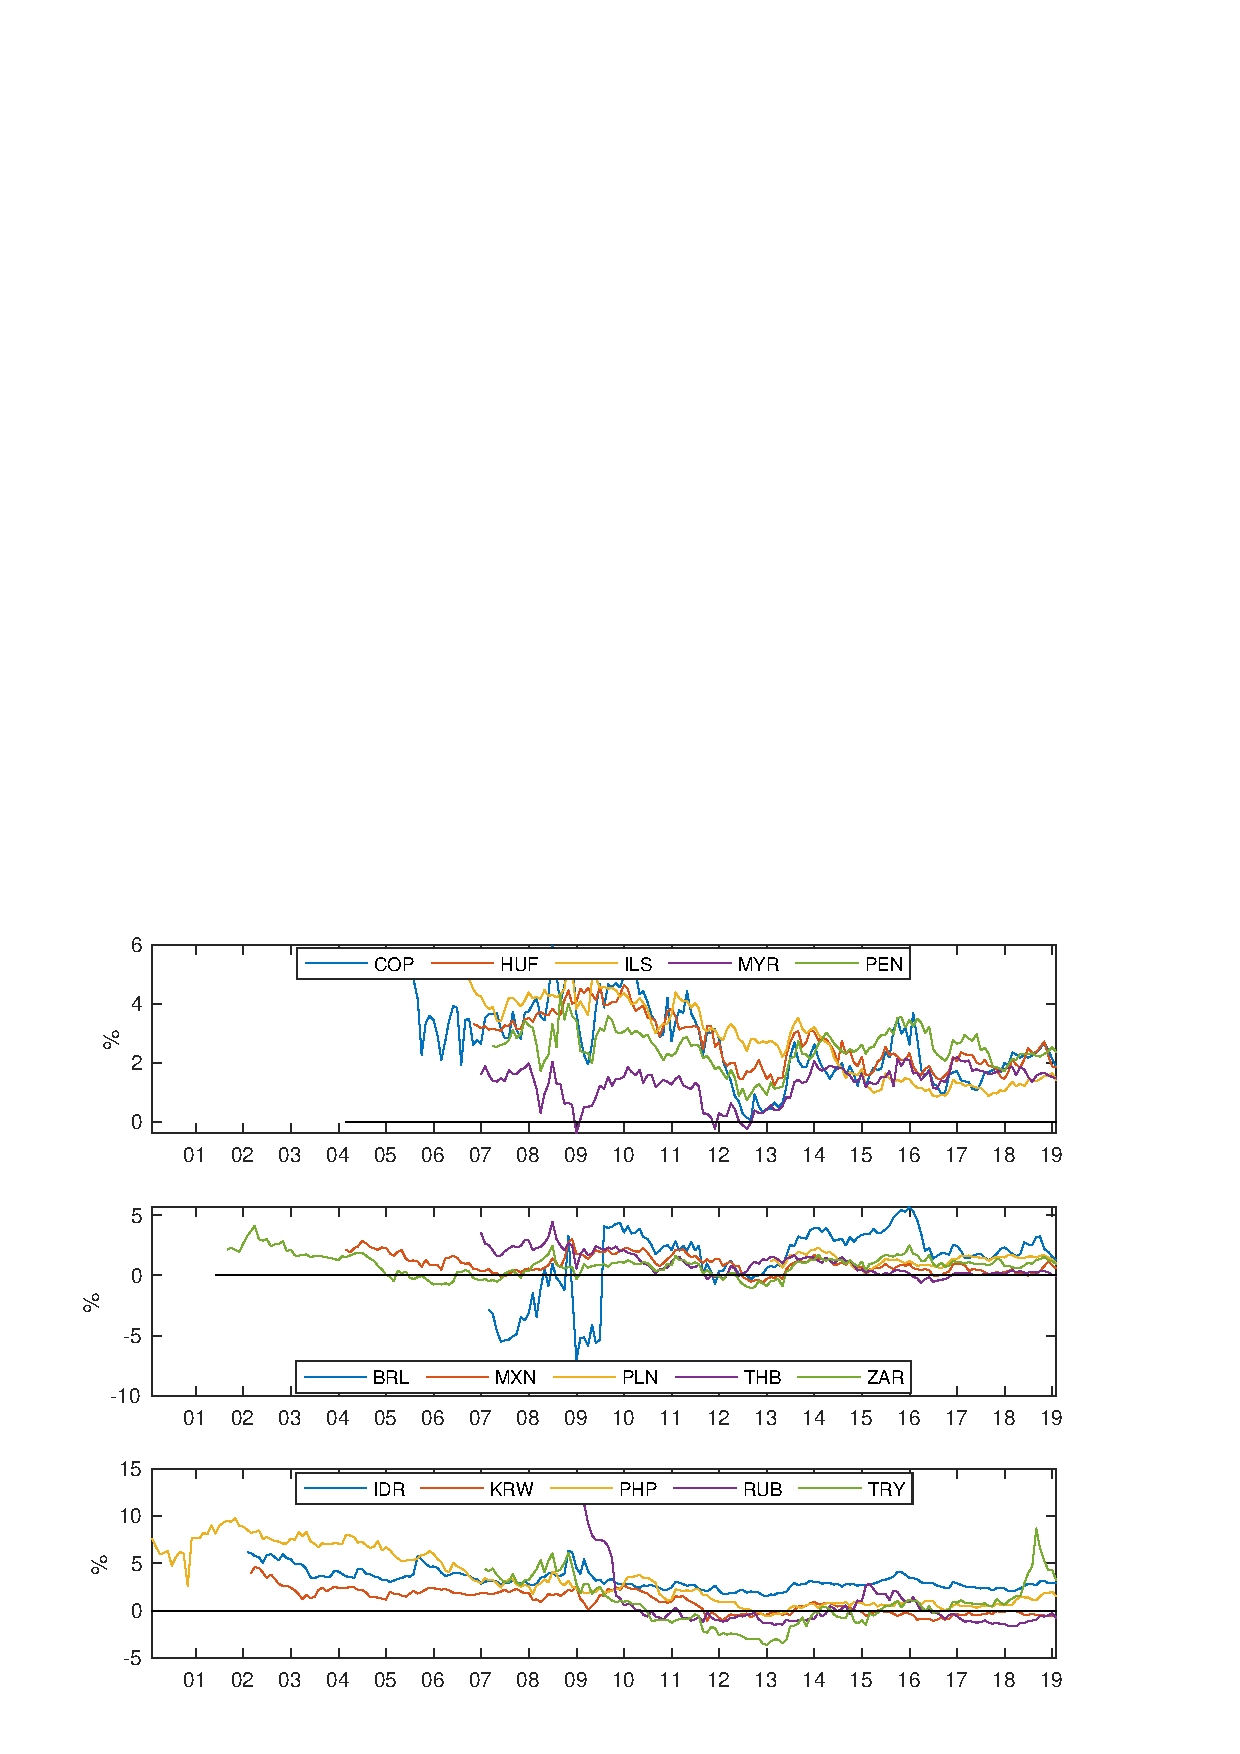
\includegraphics[width=1\textwidth,height=0.7\textheight]{../Figures/Temp/temp_tp10yrEM}
			\par\end{centering}
		\caption{Estimated 10-Year Term Premia: Emerging Markets.}\label{fig:temp_tp10yrEM}
	\end{figure}
%
%Special cases include that of Brazil whose term premium turn negative around the Great Recession and that of Russia whose term premium declined considerably. These cases might be reflecting local conditions and deserve further analysis. Consider, for example, the case of Turkey towards the end of the sample, where relevant events in 2018\footnote{On June 24, 2018, Recep Tayyip Erdogan won the presidential election. On October 2, 2018, the journalist Jamal Khashoggi disappeared after he visited the consulate of Saudi Arabia in Istanbul.} translated into a higher term premium.
%
% In addition to Brazil, Russia and Turkey, the term premia of most Asian countries has been in negative territory for some period of time. Moreover, with the exception of Brazil and South Africa, the term premia of emerging markets being negative is a phenomenon observed after the Great Recession.
%
%%To summarize the figure, Table \ref{tab:rp_stats} shows the mean of the 5-year synthetic yields and summary statistics for the estimated 5-year term premia. The means of the synthetic yields fluctuate between $2.3\%$ and $10.5\%$, while the means of the risk premia fluctuate between $-36$ basis points to $150$ basis points. On average, the term premium represents around $12\%$ of the synthetic 5-year yield. For Indonesia, Russia, South Africa and Turkey the standard deviation of their term premia is relatively high compared to their mean. Philippines and Russia had periods with a really negative term premia in October 2000 and the first half of 2015, respectively; excluding those episodes, the term premium has fluctuated between $-3.5\%$ and $5.5\%$.
%%	\begin{table}
	\centering
\begin{tabular}{l|cccccc}
\toprule
\multicolumn{1}{c}{}& &\textbf{Yield}&\multicolumn{4}{c}{\textbf{Risk Premium}}\\
\cmidrule(l{.9em}r{.9em}){4-7}
%\cmidrule(lr){3}  \cmidrule(lr){4-7}
\multicolumn{1}{c}{}&\textbf{Obs}&\textbf{Mean}&\textbf{Mean}&\textbf{Std}&\textbf{Min}&\textbf{Max}\\\midrule
{ COP}&154&6.23&1.33&1.21&-0.96&4.41\\\
{HUF}&138&3.71&0.31&0.67&-0.95&1.50\\\
{IDR}&205&8.97&0.52&1.03&-3.06&3.92\\\
{ILS}&146&2.35&1.01&0.63&0.23&2.78\\\
{MXN}&173&6.22&0.88&0.74&-0.62&2.41\\\
{PEN}&141&4.64&1.50&1.55&-3.46&5.54\\\
{PHP}&219&6.54&1.21&1.25&-11.34&3.69\\\
{PLN}&157&3.33&0.64&0.52&-0.61&1.80\\\
{TRY}&155&10.52&-0.36&1.34&-3.22&2.29\\\
{KRW}&219&3.00&0.54&0.72&-1.09&3.51\\\
{MYR}&136&2.67&0.36&0.43&-0.66&1.31\\\
{RUB}&144&7.87&-0.13&1.88&-8.87&3.90\\\
{THB}&137&2.40&0.64&0.79&-1.03&2.89\\\
{ZAR}&218&8.38&0.45&1.12&-3.02&2.25\\ \bottomrule
\end{tabular}
\\
\caption{Summary Statistics: 5-Year Yield and Risk Premium.}\label{tab:rp_stats}
\end{table}
%
%For comparison purposes, Figure \ref{fig:temp_tp10yrAE} shows the 10-year term premia estimates for advanced economies using synthetic yield curves. A clear downward trend is observed for all countries. This is consistent with the empirical evidence that uses nominal yield curves; \cite{Wright:2011} shows a declining trend in term premia for most of these countries going back to the 1990s and argues that it reflects a reduction in inflation uncertainty.
%		\begin{figure}[!htbp]
		\begin{centering}
			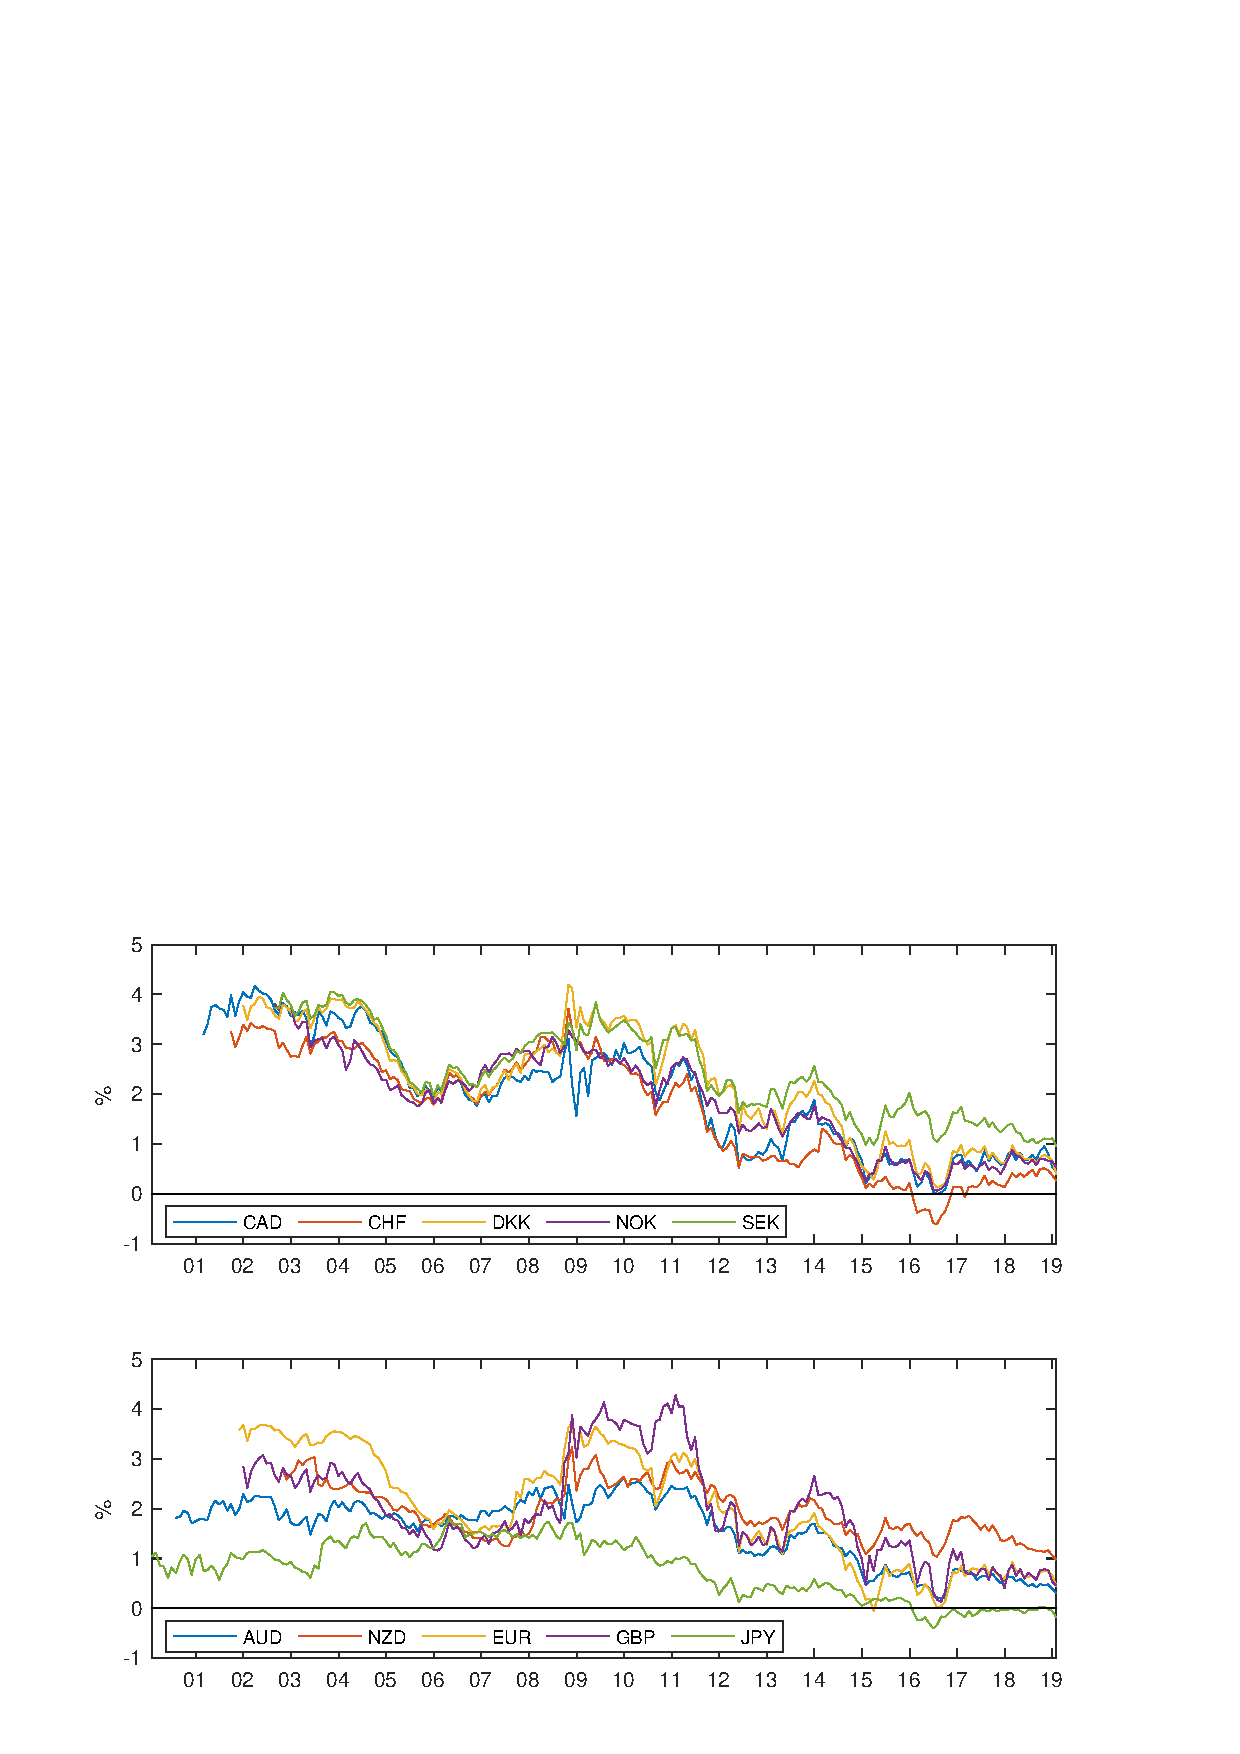
\includegraphics[width=1\textwidth,height=0.45\textheight]{../Figures/Temp/temp_tp10yrAE}
			\par\end{centering}
		\caption{Estimated 10-Year Term Premia: Advanced Economies.}\label{fig:temp_tp10yrAE}
	\end{figure}
%
%Note that although the term premia of most advanced countries seem to reflect a common factor, that of Japan behaves differently probably reflecting the fact that Japan was at the zero lower bound before the other countries.
%
%According to KW, the 10-year term premium estimate for the U.S. has been negative for most of the time since mid-2011, fluctuating between $-1$\% and $0$. Of the advanced countries considered, only Switzerland and Japan have experienced more than one month with a negative term premium, compared to several emerging markets, mainly Korea, Russia and Turkey. In particular, before the taper tantrum there was a tendency of declining term premia for emerging markets, which for some countries actually turned out negative.
%
%\subsubsection{Term Structure of Term Premia}
%In addition to comparing the term premia across countries, one can also compare them across maturities per country. In general, the term premium increases with maturity. As one would expect, when long-term bonds are seen as riskier than short-term bonds, investors would require a higher compensation for holding long-term bonds. This pattern, however, is not universal as can be seen in Figure \ref{fig:temp_ts_tp} in the Appendix, which shows two examples of this, namely Korea and Mexico. Therefore, the exceptions for the general pattern are observed in both emerging and advanced countries since the KW estimates also show that after the Great Recession, the 1-year U.S. term premium has been above the 5- and 10-year term premia at some points.
%%\footnote{Sometimes, the standard deviation of the term premia increases with maturity.}
%%		\begin{figure}[!htbp]
		\begin{centering}
			\vspace{12.5mm}
			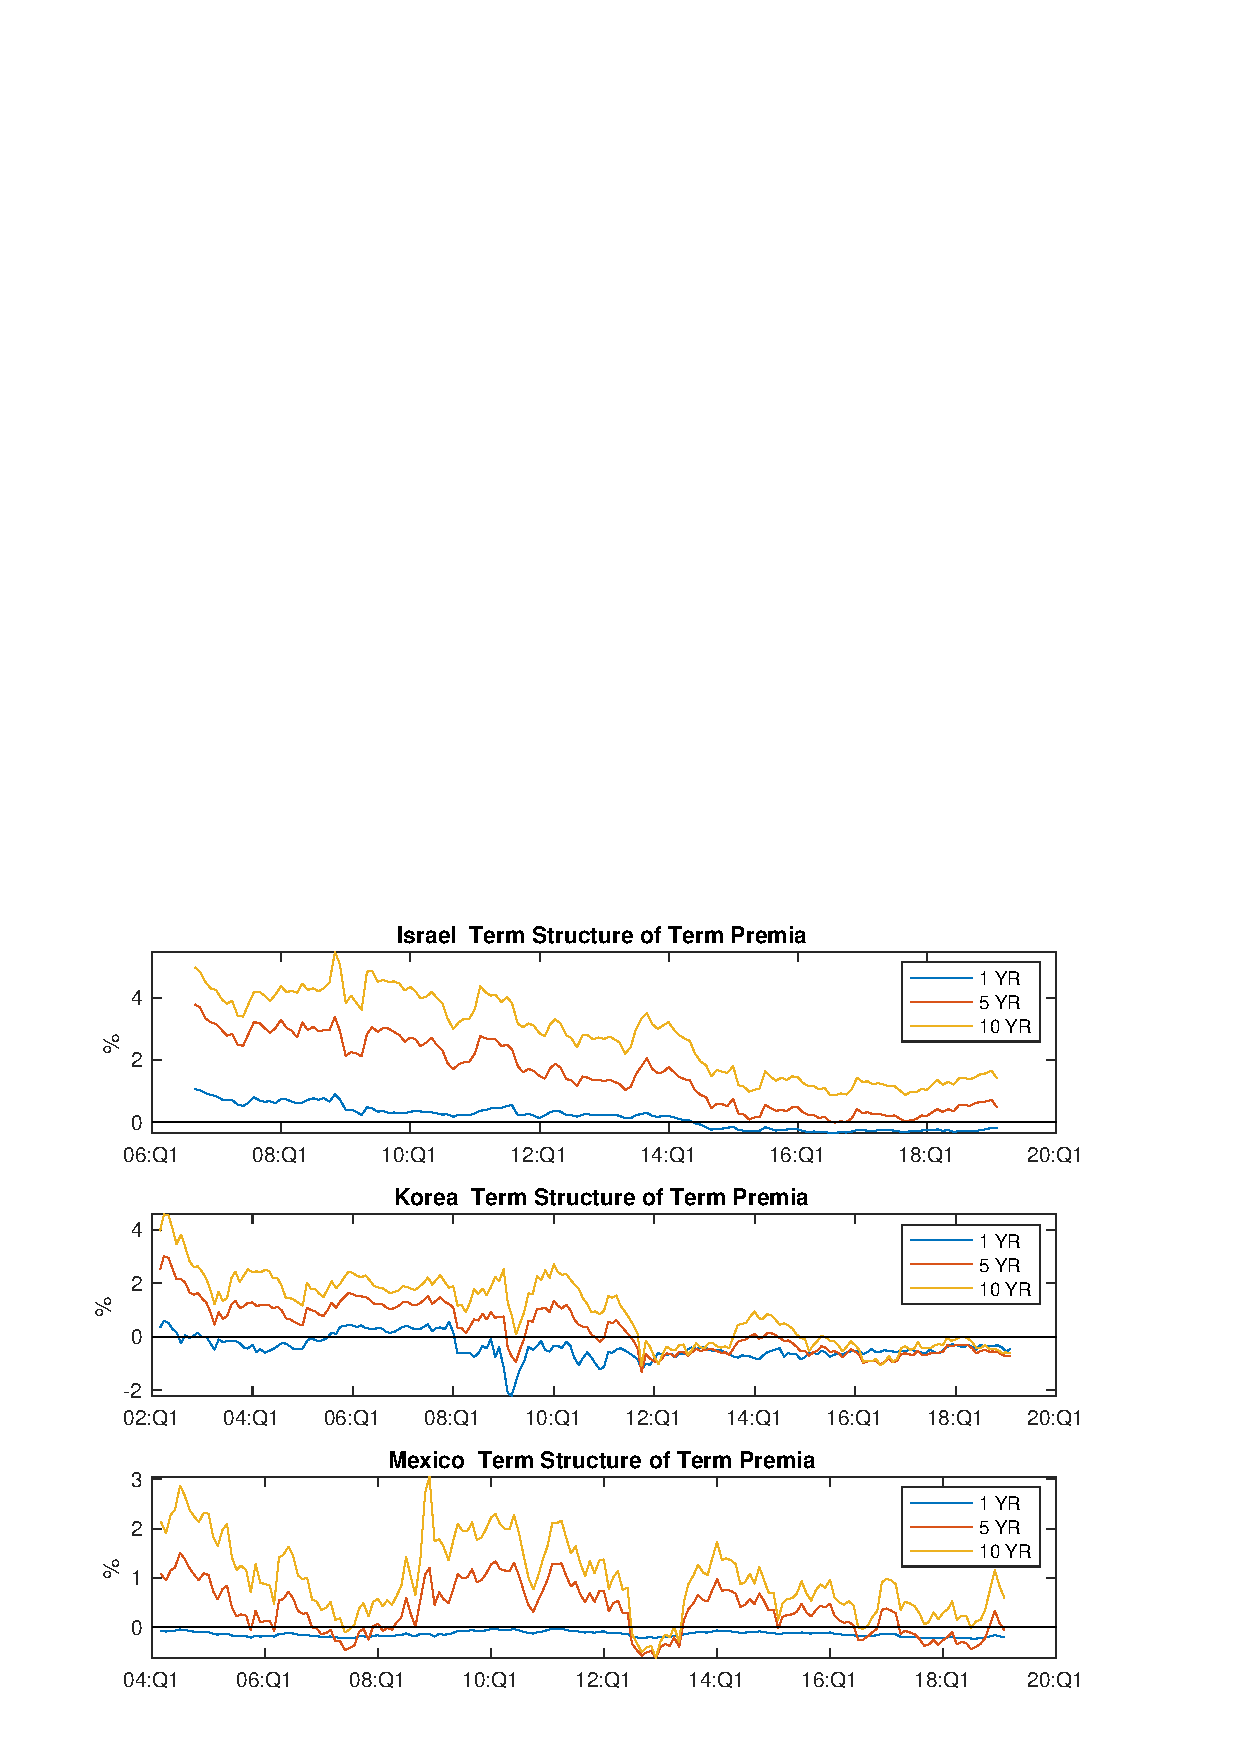
\includegraphics[width=1\textwidth,height=0.8\textheight]{../Figures/Temp/temp_ts_tp}
			\par\end{centering}
		\caption{Estimated Term Premia for Different Maturities.}\label{fig:temp_ts_tp}
	\end{figure}
%
%\subsubsection{Common Factors in Term Premia}
%To see whether there are common factors influencing the term premia in emerging markets, Table \ref{tab:temp_tp_common} shows the proportion of the total variation in the 10-year term premia explained by their first three PCs. To consider all countries, the starting date is December 2006. The first three PCs explain more than $80\%$ of the variation in the term premia of emerging markets and more than $98\%$ for advanced countries. This evidence highlights the importance of considering global factors as drivers of the term premia. But at the same time, the evidence for emerging markets shows that both domestic and common factors seem to be at play as drivers of their term premia.
%%	\begin{table}
	\centering
\begin{tabular}{l|cccc}
\toprule
&\textbf{PC1}&\textbf{PC2}&\textbf{PC3}&\textbf{Sum}\\\midrule
{ Since Nov 2016} - All Countries&40.29&23.62&12.37&76.28\\\
Since Jun 2005 - 8 countries&52.46&16.66&12.08&81.19\\ \bottomrule
\end{tabular}
\\
\caption{Proportion of Total Variance in 5yr RP Explained by First 3 PCs.}
\label{tab:pc_common}
\end{table}

%%	\begin{footnotesize}\begin{table}\centering\begin{tabular}{l|cccc}
\toprule
\multicolumn{1}{c}{} &\multicolumn{2}{c}{EM TP}&\multicolumn{2}{c}{Residual}\\
\cmidrule(l{1.1em}r{1.1em}){2-3} \cmidrule(l{1.1em}r{1.1em}){4-5}
\multicolumn{1}{c}{} & 5 YR & 10 YR & 5 YR & 10 YR \\
\midrule
(15) Dec-06 & 67.40 & 71.67 & 62.99 & 58.25 \\(8)  Jul-05 & 79.57 & 82.65 & 74.36 & 76.40 \\(4)  Latam & 95.43 & 94.96 & 94.01 & 92.47 \\(5)  Asia & 90.19 & 91.43 & 88.52 & 87.98 \\(4)  Europe & 97.38 & 95.25 & 97.15 & 93.38 \\\bottomrule\end{tabular}\caption{Percent of Total Variance Explained by First 3 PCs.}\label{table:CmnFctrs}\end{table}\end{footnotesize}
%	\begin{tiny}\begin{table}\centering\begin{tabular}{l|cc}\toprule & Dec-2006 \\\midrule EM & 81.01 \\AE & 98.07 \\\bottomrule\end{tabular}\caption{Total Variation Explained by First 3 PCs (\%): 10-Year Term Premium.}\label{tab:temp_tp_common}\end{table}\end{tiny}
%
%\subsubsection{Survey-Based Term Premia}
%As already mentioned, one way to check the term premia estimates obtained from affine term structure models is to use survey data since long-term surveys of professional forecasters can be used to obtain a model-free estimate of the long-term term premium. Using this approach, the term premium is calculated as the difference between the long-term interest rate and the survey-expectation of the future short-term interest rate over the same horizon. Since the long-term expectations of the policy rate for emerging markets are not provided by Consensus Economics, they are approximated as explained in section \ref{sec:SurveyData}. As it is also explained in that section, given the persistence of bond yields, surveys can also provide information to help in the identification of the term premium.
% It is important to acknowledge, however, that surveys might not represent the market expectations or the expectations of the marginal investor.
%
%Figure \ref{fig:temp_tp10yrSvy} displays the 10-year (long-term) term premium estimated in this way for most of the emerging markets considered in Figure \ref{fig:temp_tp10yrEM}.
%		\begin{figure}[!htbp]
		\begin{centering}
			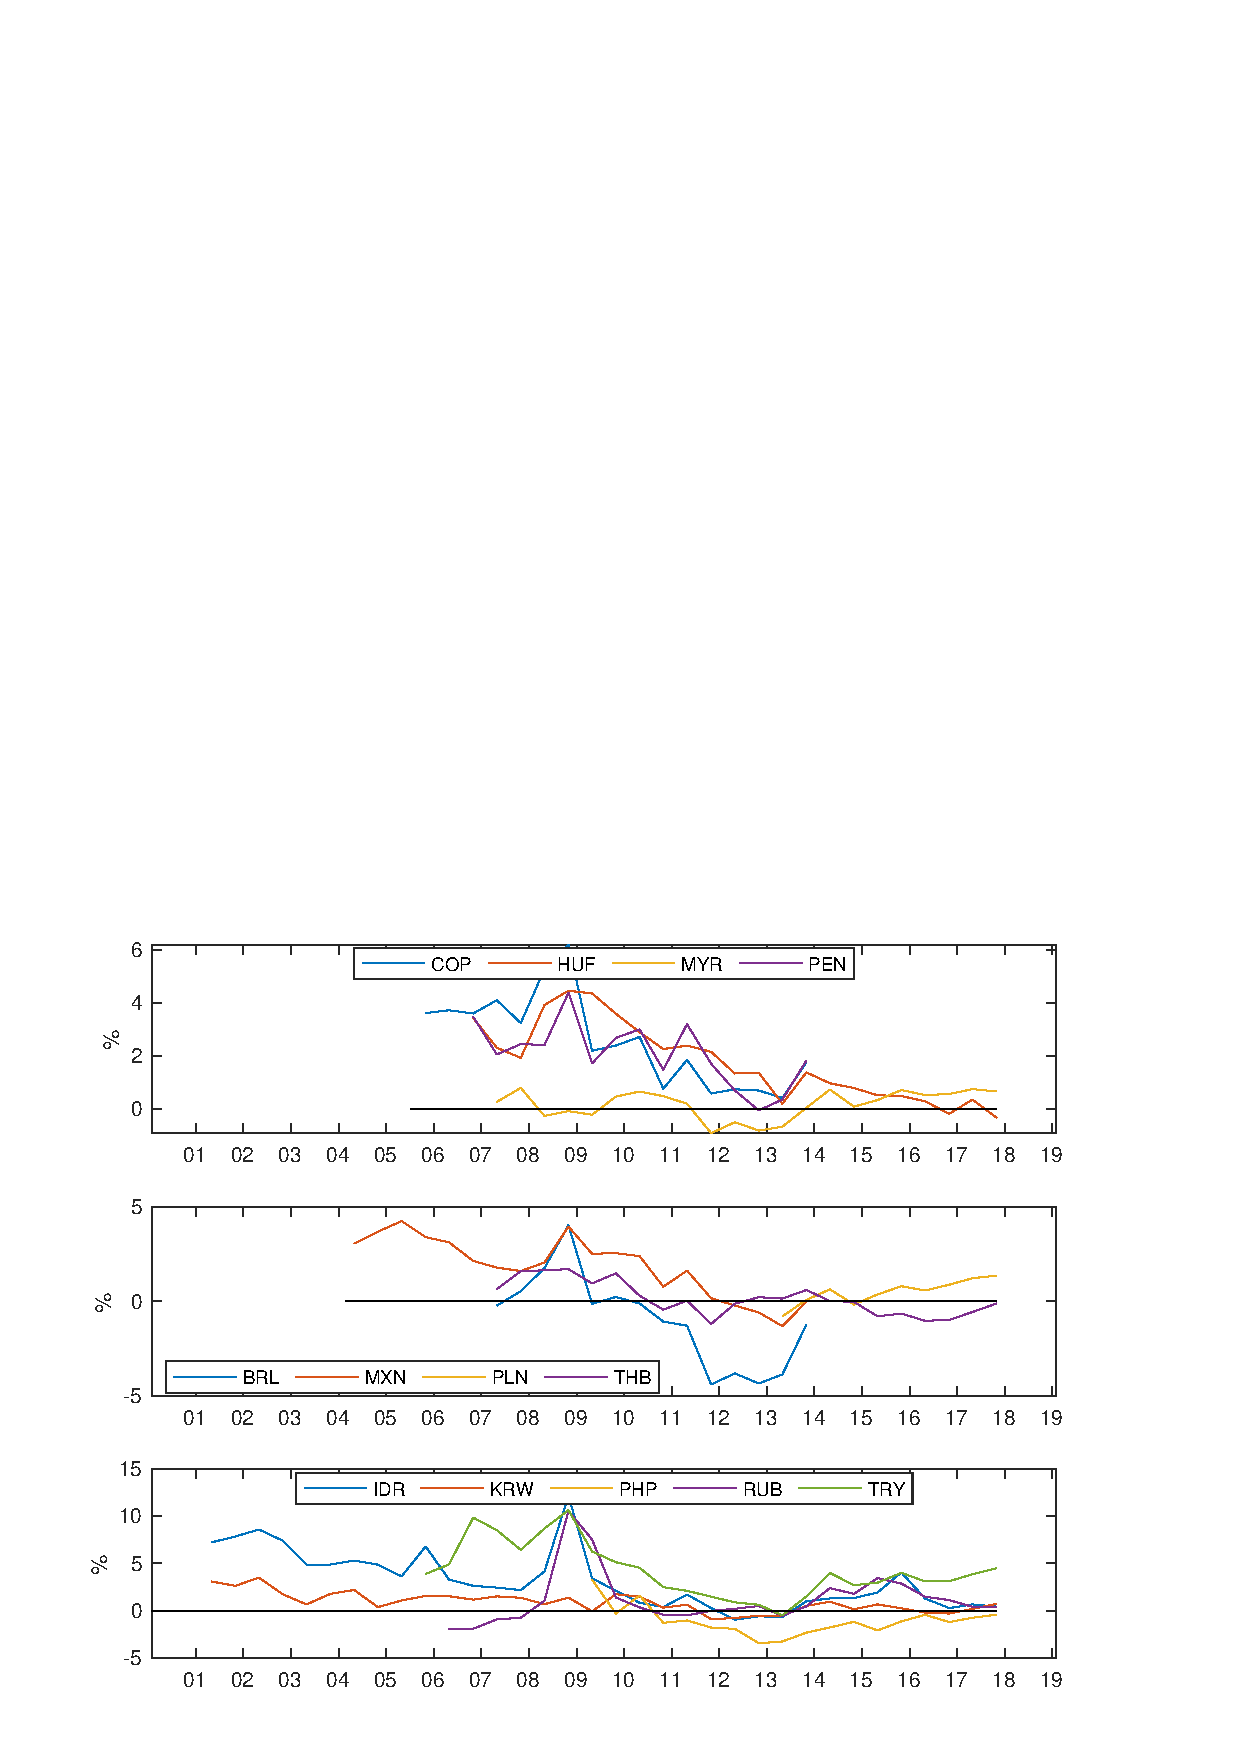
\includegraphics[width=1\textwidth,height=0.5\textheight]{../Figures/Temp/temp_tp10yrSvy}
			\par\end{centering}
		\caption{Survey-Based 10-Year Term Premium Estimates}\label{fig:temp_tp10yrSvy}
	\end{figure}
%
%With the exception of Brazil during 2012-13, the term premia estimated using survey data are in line with the model-based term premia. In fact, the average correlation between the two is $80.4\%$.\footnote{Even for the term premia calculated using the nominal yield curve, the correlation with the survey-based term premia is equal to $85\%$.} This is reassuring and supports the idea of supplementing the term structure model with survey data to better pin down the term premia in emerging markets, which will in turn provide a more robust decomposition of the nominal yield curve. This will be done in future versions of this paper.

	
}{}	% Closes \iftoggle{fulldraft}


\section{Understanding the Yields of Emerging Markets} \label{sec:analysis}
\iftoggle{toclinks}{\gototoc}{} % Turn it on/off in packages.tex, command in macros.tex
\iftoggle{cboxes}{	   				  % Turn it on/off in packages.tex
	\begin{boxeditems}
		\item Commonalities (TPs, yP, LCCS) all, ST vs LT.
\end{boxeditems}}{}

This section documents a strong and persistent response of the sovereign yields of emerging markets to U.S. monetary policy shocks. 
It  also analyzes how each component of the yields reacts to the news, and highlights that the response depends on the type of shock. %information conveyed.

\iftoggle{fulldraft}{					% Turn it on/off in packages.tex

\subsection{Comovement} \label{sec:globalPC}
\iftoggle{toclinks}{\gototoc}{} % Turn it on/off in packages.tex, command in macros.tex

%Here, I exploit it to provide new stylized facts about them that will help to interpret the results in the next section.

The response of emerging market yields to U.S. monetary policy shocks in part depends on the extent to which LC bonds are integrated to the global financial markets.
This requires to answer the question of how connected are the sovereign yields of emerging markets.
One way to address this question is to pool all yields together and see whether there is a global-level factor, associated with the first principal component.
For advanced countries, a global factor explains more than 90\% of the variation in their yields, consistent line with \cite{DahlquistHasseltoft:2016}.
In contrast, a global factor explains only around 50\% of the variation in emerging market yields or their components.
%\footnote{ \cite{DuSchreger:2016JoF} find something similar for the credit risk premium.}
%This suggests that the emerging market yields are not as connected among themselves as the yields of advanced countries.
%When yields are separated by maturity, a similar pattern emerges for the 1-year yields, whereas for the 10-year yields, a global factor explains around 95\% in AEs and 40\% in EMs. 
%Although a global factor plays a role in the variation of yields in both AEs and EMs, the bond yields in EMs are not as tightly connected as they are in AEs.
%These percentages are largely the same after the GFC.
%A global factor explains around 40\% of the variation of all the three components of yields in EMs.\footnote{ \cite{DuSchreger:2016JoF} also show that the credit risk premium has a low reaction to global variables.} 
%For AEs, in contrast, a global factor explains 90\% of the variation in the expected short rate and 80\% in their term premia. 
%After the GFC, these percentages **increased** for the term premia in AEs and for the two components of the synthetic yields in EMs.

A more formal way to answer the question is to measure the degree of connectedness among emerging market yields.
%; that is, how much does the shock in one market has implications for the other markets.
\cite{DieboldYilmaz:2014} propose a system-wide measure of connectedness 
%based on forecast error variance decompositions.
%Their methodology 
that assesses shares of forecast error variation in a country's bond market due to shocks arising elsewhere.
Following \cite{ACDM:2019} and \cite{BostanciYilmaz:2020}, I obtain the connectedness index using a vector autoregression of order 1, with a forecast horizon of 10 days and a rolling window of 150 days for the daily changes of the 10-year nominal yields 
%of the emerging markets in the sample 
and each of their components.
Figure \ref{fig:dyindex10y} displays the connectedness index for emerging and advanced countries.
%\footnote{ The index for emerging markets has a shorter history because its computation requires a balanced panel. Also, since the construction of the synthetic curve does not involve nominal yields, the history of the components do not start on the same date.} 
The index for emerging markets (figure \ref{subfig:dyindex10yEM}) captures some developments of the European sovereign debt crisis in 2012 and  the Greek debt crisis in 2015.
Notably, it spiked above 55\% around the taper tantrum episode in 2013.\footnote{ During the episode, financial markets feared an earlier than expected withdrawal of the Fed's unconventional stimulus measures.} %and remained elevated for about a year.
The second biggest spike %in the index 
occurred after the 2016 U.S. presidential election.
%, with potential implications for some of the emerging markets in the sample.
By mid-2017, the index was back to its pre-taper tantrum levels of around 30\% compared to an average value of the index for advanced countries of close to 70\%.

The difference between the highly connected yields of advanced countries and the low connected yields of emerging markets might seem at odds with the idea of a 
%perspective based on the 
global financial cycle \citep{Rey:2013}.
%On the one hand, the yields of advanced countries are highly connected among themselves (see figure \ref{subfig:dyindex10yAE}), which over the last decade has been driven by an increase in the connectedness of their term premia, as documented by \cite{ACDM:2019}.
%Changes in the compensation for risk in one advanced country not only spillover to other advanced countries but they have become increasingly important for the variation in their yields.
%On the other hand, the yields among emerging markets are not as connected as those in advanced countries (see figure \ref{subfig:dyindex10yEM}).
The level of the index for emerging markets is about half the level of the index for advanced countries, it shows no upward trend for either their nominal yields or their components.\footnote{ \cite{ACDM:2019} already document that the increase in the connectedness of the yields of advanced countries has been driven by an increase in the connectedness of their term premia.}
% of emerging market yields do not show a clear trend, their relative importance seems to depend on the current economic environment.
%as might be expected under a perspective based on the global financial cycle. %according to the idea of the
%Is there a component that is more connected? 
%Unlike the rise in the connectedness of the term premium among advanced countries, 
These results, however, are consistent with the global financial cycle in which the global bond markets operate under a core-periphery structure, in which the bond markets of advanced countries constitute the (highly interconnected) core and those of emerging markets represent the (less connected) periphery.
Countries in the periphery are in turn connected to the network mainly through countries in the core.\footnote{ The core-periphery structure has been shown to be a good description of different networks in economics and finance. For example, \cite{CvP:2014} show that the interbank market operates under such a structure.}
According to this, figures \ref{subfig:dyindex10yEM} and \ref{subfig:dyindex10yAE} are measuring the connectedness of the periphery and the core, respectively.
Therefore, what matters for emerging market yields are not spillovers originating in other emerging markets but in advanced countries, which makes the argument of a global financial cycle stronger, not weaker.

%Are the short and long end equally connected?
%Diebold-Yilmaz index for 2Y and 10Y to test Obsfeld vs K-O
A related question is whether the connectedness of yields is the same throughout the term structure or whether some sections of the curves are more connected than others.
%The role of a global factor seems to be different throughout the yield curve.
\cite{Obstfeld:2015} 
%shows that the effects of the global financial cycle are different at the short than at the long end of the yield curve. In particular, he 
argues that long-term bonds are more globally connected than short term ones.
On the other hand, \cite{Kalemli-Ozcan:2019} argues that short-term yields suffer more the effects of global influences.
%When yields are separated by maturity, a global factor explains around 50\% of the variation in the 1-year yields of EMs, compared to 90\% for AEs. 
%For the 10-year yields, a global factor explains around 60\% of the variability in EMs, relative to 95\% in AEs. 
%However, the role of the global factor is larger for the two components of the synthetic yield curve in the long end than for the short end.
%In sum, the role of a global component is larger for long-term yields and its components.
Figure \ref{fig:dy_index_ts} plots the connectedness index for different maturities.
It shows that the long end is relatively more connected than the short end, similar to what is observed for advanced countries, although this pattern became relevant for emerging markets after the taper tantrum episode.
The figure also shows that the connectedness of the short end of the yield curves is similar between advanced and emerging markets.
The difference in connectedness between two groups of countries is therefore driven by the medium and long end of their yield curves.
Although foreign participation in LC bond markets has increased, it is still mostly held by local investors, especially medium- and longer-term bonds as suggested by figure \ref{fig:dy_index_ts}, 
%of emerging markets are far from being fully integrated in the global financial markets 
and are therefore more responsive to local factors.
%In sum, while the yields of emerging markets are indeed globally connected, they are less so than the yields of advanced countries. 
%In particular, 
%Several factors can explain these patterns, including segmented markets, capital controls, home bias and regional differences.
%therefore seem to play a bigger role in the yields of EMs, and its components, than they do for AEs.


\subsection{Drivers} \label{sec:Drivers}
\iftoggle{toclinks}{\gototoc}{} % Turn it on/off in packages.tex, command in macros.tex

%To what extent US YC is related to EM yield components?
I start by studying the role of the components of the U.S. yield curve as drivers of emerging market yields and their components.
%cyclical properties of the nominal yields 
To do this, I use the decomposition based on the \cite{KimWright:2005} model, who address the small sample problem with survey forecasts of future interest rates.
%start the analysis of the relationship between U.S. monetary policy and the sovereign yields of emerging markets, I run panel data regressions of those yields on the components of the U.S. yield curve controlling for a variety of  variables.
%At the same time, those regressions allow me to study the cyclical properties of  emerging market yields. The coefficients of interest are those associated with 

To understand the potential drivers of emerging market yields in general, I run the following regressions 
\begin{equation} \label{eq:nPanelDCMP}
	\eqpanelTPreg .
\end{equation}
\noindent for country \(\idxi\) in month \(\idxt\), where \(\alpha_{\idxi}\) are country fixed effects, \(z_{\idxspnl}\) is a vector of global and domestic variables that are likely to drive emerging market yields, and \(u_{\idxspnl}\) is the error term. 
%Fed decisions influence monetary conditions abroad \citep{Rey:2013}, its policies affect the future expected value of its policy rate as well as the compensation for interest rate risk (the term premium), whose effects can in turn spillover to domestic yields.
The dependent variables \(\yld_{\idxspnl}\) the nominal and synthetic yields, the three components of the nominal yields and the forward premium\footnote{ Remember that synthetic yields add the forward premium to the U.S. yield curve.} for the 2- and 10-year maturities.
%, namely the expected future short rate, the term premium and the credit risk premium. 
%The dependent variable in the last column of the table is 
%, and so it is included to assess whether its behavior mirrors that of any of the components.
%As can be seen, the components have different dynamics, they are not associated to the same variables nor in the same magnitudes.
%Also, none of them can be inferred from the forward premium as it behaves differently to %does not mirror % directly tied to 
%any of them.

Other potential drivers of the yields include 
%global financial and domestic macroeconomic and financial variables.
%The variables considered to capture global financial conditions are 
the Cboe's volatility index (Vix) and the S\&P \(500\) stock market index. 
The Vix reflects the implied volatility in option prices and is usually considered as a measure of risk aversion and economic uncertainty; given the sudden spikes in the index, it is common to use it in logs.
The global version of the EPU index by \cite{BakerBloomDavis:2016} is used as an alternative measure of global uncertainty.
Variables reflecting global real economic activity are the price of oil and the index of economic activity based on world industrial production proposed by \cite{Hamilton:2019}.
%The VIX and the federal funds rate have been used in the global financial cycle literature \citep[see][]{Rey:2013} to study the effects of common factors on capital flows. The VIX is usually used as a measure of risk aversion and economic uncertainty and the fed funds rate is a measure of the monetary policy stance in the U.S. 
%For the U.S. monetary policy, the variable used is the effective federal funds rate calculated by the New York Fed.
Inflation and unemployment rates capture domestic macroeconomic conditions in each country.
%year-on-year percentage change in the consumer price index
%The domestic variables include inflation, the unemployment rate and industrial production to capture macroeconomic effects. 
Finally, the exchange rate (LC per USD) is included to rule out explanations of changes in yields based on currency movements.
%and the local stock market index are included as measures of local financial conditions.
Monthly returns for the stock market index, the oil price and the exchange rate are calculated as the log difference of the series, and expressed in basis points.

Tables \ref{tab:ycdcmp2y} and \ref{tab:ycdcmp10y} report the results for the full specification of the model.\footnote{ The effects of the variables remain broadly similar across specifications of the model that exclude some of the regressors for each dependent variable.} 
%that includes all of the potential drivers.
%In terms of drivers, 
The role of the components of the U.S. yield curve %play a significant role for emerging market yields, highlighting the 
already indicate potential spillover effects from the Fed's policy decisions to emerging market yields.
%It is worth highlighting here the direct link between the equivalent components. 
Increases in the future expected short rate in the U.S. are positively associated with future expected policy rates in emerging markets, whereas increases in the U.S. term premium relate to increments in the term premia of emerging markets.
Moreover, the association between the U.S. components and the synthetic yields is larger than with the nominal yields. This in turn explains the negative association of the U.S. components with the credit risk premium.
Larger increases in synthetic relative to nominal yields, mechanically decrease the credit risk premium.
Therefore, the trade-off between explicit and implicit defaults highlighted before can be seen in table \ref{tab:ycdcmp10y} through the connection between the U.S. term premium and the credit risk premium.
In addition, there are also cross effects. 
The expected short rate in emerging markets reacts to changes in the U.S. term premium. 
This is consistent with the U.S. risk spillovers channel described by \cite{Kalemli-Ozcan:2019}.
The signs for the rest of the drivers are correct.


%More generally, external conditions have a relevant impact on domestic bond markets, consistent with the view of a global financial cycle.
%The U.S. term premium, the Vix and the U.S. stock market are linked to the different components of emerging market yields.\footnote{ On the other hand, once controlling for the other factors, the price of oil and the global EPU index play no role in explaining yield dynamics.}
%They are particularly associated with the credit risk premium, 
%%is global financial conditions given by the Vix, the U.S. term premium and the U.S. stock market.
%but they do not seem very helpful in providing information about default risk in emerging markets given their low explanatory power (in terms of the R-squared statistic) relative to the other yield components.
% since  explain a relatively lower percent of the premium's variability.


%In this case, the effect is similar among all countries.
%On average, the 10-year U.S. term premium explains around 40\% of the variation in the expected short rates in both EMs and AEs.
%Moreover, for EMs, the 10-year U.S. term premium explains more of the variation of the expected short rate than the U.S. expected rate itself. % unlike the case for AEs before GFC
%After the GFC, the 10-year U.S. term premium explained more than the U.S. expected rate in both AEs and EMs.

The results shows that inflation and unemployment are key domestic variables.
The evidence in table \ref{tab:ycdcmp10y} suggests that the term premia in emerging markets is countercyclical.
Investors demand a higher term premium during recessions, when the unemployment rate increases. 
Moreover, the positive association between inflation and the term premium conforms with the idea that inflation erodes the value of nominal bonds and so, in periods of rising inflation investors expect the central bank to tighten its monetary stance going forward (coefficient on the third column) and demand a higher term premium (coefficient on the fourth column). 
More generally, changes in inflation are associated with changes in all of the dependent variables except for the credit risk premium. 
In particular, the magnitudes are similar for nominal and synthetic as well as for the forward premium.

Lastly, there is evidence on the risk-taking channel of exchange rates documented by \cite{HofmannShimShin:2019}.\footnote{ According to the standard view based on the trade-channel effect, a depreciation is expansionary because it stimulates exports and discourages imports, increasing the trade balance.} 
Accordingly, a currency appreciation is associated with easier financial conditions and compressed sovereign bond spreads.
However, here it works through the term premium instead of the credit risk premium as they argue.
%The two main domestic factors are . Holding the other factors constant, an increase in any of these three variables increases the term premia in emerging markets. 
%The effect of the domestic variables is in line with what has been found for advanced countries using nominal yield curves. 

In closing, the yield decompositions provide valuable information on the driving forces behind the sovereign yields of emerging markets.
Nevertheless, it is important to acknowledge that the model in equation (\ref{eq:nPanelDCMP}) may suffer from econometric problems such as endogeneity as well as the use of persistent the variables.
These issues are addressed next.

\subsection{Response to U.S. Monetary Policy} %\label{sec:spillovers}

\subsubsection{Shocks} \label{sec:USMPS}
\iftoggle{toclinks}{\gototoc}{} % Turn it on/off in packages.tex, command in macros.tex

\cite{GSS:2005a} and \cite{Swanson:2018} show that monetary policy has more than one dimension since asset prices respond to different types of news about monetary policy.
This paper considers three types of U.S. monetary policy shocks, namely
unexpected changes to the current policy rate \citep{Kuttner:2001}, surprise changes to the future path of the policy rate \citep{GSS:2005a}, and unanticipated announcements about the Fed's LSAP programs \citep{Swanson:2018}. 
They will be referred to hereinafter as target, path and LSAP shocks, respectively.

The shocks are identified using high-frequency data around Fed's monetary policy announcements.
These shocks are essentially surprises in monetary policy decisions that represent a change in the information set of market participants \citep{GurkaynakWright:2013,NakamuraSteinsson:2018JEP}.
The construction of the shocks therefore requires to calculate the change in asset prices that capture market expectations of monetary policy decisions.
These changes are measured in windows containing monetary policy decisions starting 15 minutes before to 1 hour and 45 minutes after each Federal Open Market Committee (FOMC) meeting since 2000 giving a total of 162 events.\footnote{ It is common to exclude from the analysis the meeting of September 2001 that followed the terrorist attacks earlier in the month, see \cite{GSS:2005a} and \cite{NakamuraSteinsson:2018JEP}.}
In days with no FOMC meeting, the shocks are set to zero.
The dataset only includes monetary policy announcements.
The dataset by \cite{FerrariKearnsSchrimpf:2017} also includes the release of minutes and speeches by Fed officials.

The assets used to measure the monetary policy shocks are the current federal funds rate future (FF0) contract, the 8-quarters ahead eurodollar future (ED8) contract and the yield of the 10-year U.S. Treasury bond.
The target shock uses rescaled changes in the price of the FF0 contract; I follow \cite{GSS:2005a} who implement an intraday version of the daily measure proposed by \cite{Kuttner:2001}.
The price change in the ED8 contract is a measure of surprises in the federal funds rate two years into the future.
The path shock is the residual of a regression of the intraday change in the ED8 contract on the target shock; this shock is highly correlated with the path factor in \cite{GSS:2005a}.\footnote{ The change in the 4-quarters ahead eurodollar future (ED4) contract could also be used to measure the path shocks. However, after 2011 intraday changes in ED4 became essentially zero since market participants expected the policy rate to remain at zero for at least a year.}
Finally, I follow \cite{Swanson:2018} for measuring the last type. % of shocks.
The LSAP shock is the residual of a regression of the intraday change in the 10-year yield on the target and path shocks.
A positive value in any of the shocks represents a tightening of the monetary policy stance, whereas a negative shock indicates an easing.
%Correlation of shocks?


%Sample periods for the shocks.
The relevance of the shocks has varied over time.
After 2008 the target shocks are essentially zero, since then there was no surprise changes in the current policy rate.
By contrast, the meaning of LSAP shocks is unclear before 2008.
Path shocks, nevertheless, have been relevant before and after the GFC.
As a result, target shocks are considered from 2000 to 2008, LSAP shocks are considered starting in 2009, and path shocks span the whole sample period.
%Figure \ref{fig:USmps} plots all three monetary policy shocks.
Table \ref{tab:mpsstats} reports descriptive statistics of the three types of shocks on monetary policy announcement days.
magnitude of shocks is generally less than 10 basis points.
shocks are not correlated, but on 18-Mar-2009 large easing path and lsap shocks
easing shocks are more common than tightening ones


\subsubsection{Spillovers} \label{sec:LPs}
\iftoggle{toclinks}{\gototoc}{} % Turn it on/off in packages.tex, command in macros.tex

The impact of U.S. monetary policy on emerging market yields is estimated using panel local projections for the daily changes in the yields and their components.
These regressions are useful to understand not only how the yields respond to the policy surprise at the time of the shock but over subsequent periods, see \cite{HofmannShimShin:2019} and \cite{ACDM:2019} for recent applications.

Following \cite{Jorda:2005}, the panel local projections are:
	\begin{equation} \label{eq:nPanelLP}
	\eqpanelLP,
\end{equation}	% \ref{eq:nPanelLP}
\noindent where \(\idxi\) and \(\idxt\) are respectively the country and time indexes, \(\idxh\) indicates the horizon (in days) with \(\idxh = 0, 1, \ldots, 90\),  \(\alpha_{\idxh,\idxi}\) is a country fixed effect, \(\epsilon_{\idxt}\) represents a type of monetary policy shock, \(\fx_{\idxspnllag}\) is a one-day lag of the exchange rate (LC per USD) and \(u_{\idxspnlfwd}\) is the error term.
The regressions are done for the 2- and 10-year yields and each of their components (the expected short rate, the term premium and the credit risk premium) for every type of monetary policy shock.\footnote{ By definition, the shocks are unanticipated by the market and thus there is no need to control for past or future shocks. Also, by construction, the shocks are not correlated among themselves so, there is no need to control for the other types of shocks.}

The parameters of interest, \(\beta_{\idxh}\), measure the average response of the yield (or one of its components) to a monetary policy shock at a particular horizon.
The contemporaneous effects of the shocks are obtained by setting \(\idxh = 0\) in equation (\ref{eq:nPanelLP}).
All responses are assessed relative to a one basis point increase (a tightening) in any of the shocks.

%The Pesaran test of cross-sectional independence is rejected at any significance level.
%Therefore, standard errors are computed following Driscoll and Kraay (1994), so that they are robust to heteroskedasticity, autocorrelation and cross-sectional dependence.

The response of the U.S. yields and its components to the three shocks are used as a benchmark to assess the responses of the yields of emerging markets.\footnote{ As before, the yields are from the dataset of \cite{GSW:2007}, the components come from the decomposition proposed by \cite{KimWright:2005}.}
The first column of figures \ref{fig:LPUS2Y} and \ref{fig:LPUS10Y} shows the responses of the 2- and 10-year yields, respectively, to all three shocks.
The on-impact effect of the 2-year yield to any of the three shocks is similar at around %half a basis point increase.
5 basis points for a 10 basis point increase in any of the shocks.
By contrast, the 10-year yield only increases in response to path and LSAP shocks contemporaneously, with LSAP shocks having a more than one-to-one impact.
The magnitudes are in line with previous literature.
The duration of the effects ranges from a couple of days up to a few days past a month, where the delayed response can be larger that the initial reaction, consistent with the evidence in \cite{BrooksKatzLustig:2019}.
The decomposition allows for a better characterization of the response.
For instance, one of the goals of the unconventional monetary policy tools was to influence (decrease) long-term bond yields and, in particular, the term premium \citep[see][]{Kuttner:2018}.
%\footnote{ \cite{Kuttner:2018} discusses the effects of the QE announcements on U.S. bond yields.}
The right hand panels in figures \ref{subfig:LPUS10Ypath} and \ref{subfig:LPUS10Ylsap} confirm this.
Meanwhile, the main effects of target shocks are seen on the expected short rate, especially at the 2-year maturity (middle panel of figure \ref{subfig:LPUS2Ytarget}).
Fed's decisions therefore impact both expectations about its policy rate in the future and the compensation required by investors to hold long-term bonds.
%Target shocks did not influence the 10-year yield.

I now turn to analyze how the sovereign yields of emerging markets respond to U.S. monetary policy.
%The main finding of this paper is reported in f
The first column of figures \ref{fig:LPEM2Y} and \ref{fig:LPEM10Y} shows the responses of their 2- and 10-year nominal yields, respectively, to all three shocks.
Those yields go up by about 2 basis points on-impact for a 10 basis point increase in any of the shocks.
Thus, the magnitude of the initial response is lower than the response of U.S. yields.
However, the response increases over time, it can last for up to 2 months and intensify to such an extent so as to become a one-to-one response, or even more in the case of LSAP shocks.
%In particular, the path and LSAP shocks have a larger and longer effect on EM yields. 
The response of the yields of emerging markets therefore lasts relatively longer than the response of U.S. yields.
\cite{ACDM:2019} documents a similar finding for a sample comprised mostly by advanced countries.
For the U.S., \cite{BrooksKatzLustig:2019} attribute this delayed response to a portfolio rebalancing channel.
%The evidence documented here is also consistent with said channel.

To better understand the spillover effects of the Fed's decisions on emerging markets, I leverage on the yield decompositions at the daily frequency.
The responses of each component are displayed in the second to last column of figures \ref{fig:LPEM2Y} and \ref{fig:LPEM10Y}.
Several things are worth pointing out about the response of the 2-year yield. First, no shock impacts the term premium. 
Second, the expected short rate only responds on-impact to LSAP shocks, but it has a substantial delayed response to target and path shocks.
Third, although the expected short rate and the term premium do not respond on impact to target and path shocks, nominal yields do respond but as a result of an increase in the credit risk premium.
Fed policies can therefore influence the compensation for credit risk in emerging markets.
%This is the first piece of evidence that Fed policies, through their effects on different markets, influence the compensation for credit risk in emerging markets.

Before analyzing the response of the 10-year yield decomposition, it is helpful to first look at the response of the forward premium to the shocks.
Remember that synthetic yields add a forward premium to the U.S. yield curve.
Since exchange rates are expressed in LC per USD, a decrease in the premium implies that the forward exchange rate is lower than the spot.
Figures \ref{fig:LPEMRHO} and \ref{fig:LPAERHO} show the responses of the forward premium for emerging and advanced countries, respectively.
In all cases, the forward premium declines (sometimes even one-to-one) on impact  in response to a shock but it remains below zero in subsequent days only for advanced countries, whereas there is only an on-impact response for emerging markets in general.
It is well documented that following a monetary tightening the dollar appreciates
\citep{FerrariKearnsSchrimpf:2017}.
This is consistent with a decline in the forward premium (when the spot is higher than the forward), which implies a future expected appreciation of the domestic currency.

It can now be seen how the the 10-year yield respond to monetary policy decisions by the Fed.
By construction, the effects on synthetic yields are linked to the responses of the U.S. yield curve and the forward premium for corresponding maturities.
Such responses have already been discussed above (see figures \ref{fig:LPUS10Y} and \ref{fig:LPEMRHO}).
The response of the synthetic yields is the net result of those two individual effects, which in turn will be reflected in the components of those synthetic yields, namely the expected short rate and the term premium.
The expected short rate does not respond on-impact for target or path shocks; the term premium also does not respond on-impact to path shocks, only to target shocks.
But their responses are sluggish a amplify over time.

The analysis of the 10-year yield shows that Fed's decisions not only impact the credit risk premium but that it can affect them in both directions.
The credit risk premium increases in response to target and path shocks, while decreases in response to LSAP shocks.
%The on-impact effect on all the components for the target and path shocks is zero but they point in the right directions.
%This information can nevertheless be used to the effects, the results of the exercise 
%Qualitatively 
%Understanding why 
%%the mechanism 
%will help to appreciate the non-zero on-impact responses of the components to LSAP shocks below.
But why does the credit risk premium increase in response to target and path shocks?
Because synthetic yields \textit{decline} on-impact.
The reason is that a lower forward premium means a lower compensation for a future currency depreciation, reducing the cost of borrowing in LC at the risk-free rate.\footnote{ Mechanically, synthetic yields decline because the forward premium declines by more than the increase in U.S. yields, see figures \ref{fig:LPUS10Y} and \ref{fig:LPEMRHO}.}
With an increase in the nominal yield and a decrease in the synthetic yield in response to a monetary tightening, the credit risk premium goes up (see the right panels of figures \ref{subfig:LPEM2Ytarget} and \ref{subfig:LPEM2Ypath}).\footnote{ The exchange rate risk channel proposed by \cite{HofmannShimShin:2019} can be indirectly seen here. A monetary tightening in the U.S. would appreciate the dollar and depreciate the domestic currency. A currency appreciation would associated with an increase in the credit risk premium and vice versa.}
That is, target and path shocks have opposite effects on the synthetic yield and on the credit risk premium on impact.
%In line with a previous discussion above, there is a delayed response in the expected rate and the term premium
Similarly the credit risk premium decreases in response to LSAP shocks because synthetic yields increase on impact.
Even though the forward premium still declines following a path shock (see figure \ref{subfig:LPEMRHOlsap}), since the U.S. yield increases by more (see figure \ref{fig:LPUS10Y}), the synthetic yield increases on impact, decreasing the credit risk premium. 
%decreases by the same amount leaving nominal yields unchanged on impact.
%Although the response on-impact of nominal yields seems moderate relative to how U.S. yields react, the on-impact response of their components is larger.
%Again, the expected short rate and the term premium respond with a lag for up to one month after the shock.
Therefore, the direction of the response of the credit risk premium  depends on the type of shock, but in particular on the relative responses of the forward premium and U.S. yields.
%It increases when Fed tightens and synthetic yields decline (when the decline in the forward premium is relatively larger than the increase in U.S. yields); this is what happens with target and path shocks.
%The credit risk premium decreases when the Fed tightens and synthetic yields go up (when the decline in the forward premium is relatively lower than the increase in U.S. yields); this is the case of LSAP shocks.
In any case, unlike the delayed response in nominal yields and the components of synthetic yields, the reaction by the credit risk premium is short lived.
Given that the forward premium for emerging markets only reacts on-impact, the effects on the nominal yields in the subsequent days are essentially driven by the responses of the expected short rate and the term premium.
Finally, notice that the effects on the credit risk premium can revert over time, which would explain the negative correlation reported in section \ref{sec:Drivers}.

%monetary policy shocks therefore lead to a reassessment of 
%on-impact response: direction, magnitude, plausibility, duration
%impact on components, 
%effects of each type of shocks
%explanation
%relation to literature: Bustanci-Yilmaz, Hofmann-Shim-Shin, UIP
%the yields of emerging markets are less globally connected than those of advanced economies (see section \ref{sec:globalPC}), 


%Contemporaneous event study regressions capture the on-impact response of yields to the shocks.
%Figures: response of US, EM and AE yields to each of the shocks.
%Results: delayed response, some responses are region-specific.
%The decomposition of the nominal yields can be used to see the effects of the 

%Plausibility of direction of effects. Stories for direction of effects.
%Magnitudes are reasonable?



%Figures \ref{fig:ssb_tp_QE} and \ref{fig:ny_tp_QE_AE} plot the estimated term premia for EMs and AEs, respectively, along with the dates of the announcements of the three rounds of the Quantitative Easing (QE) program, the Maturity Extension Program (MEP) and the Taper Tantrum (TT). As can be seen, term premia declined globally following the QE announcements and, in general, increased with the TT announcement.
%Even the expectation part of the short rate in some countries coincided with the UMP announcements.
%Figures \ref{fig:ssb_yP_QE} and \ref{fig:ny_yP_QE_AE}  show that, in general, expectations of future short rates declined during the QE announcements across both AEs and EMs, and increased with the TT announcement.
%	\documentclass{article}
\usepackage{graphicx}
\usepackage[margin=1in]{geometry}
\usepackage[outdir=./]{epstopdf}  					% Avoids errors when input figures
\usepackage[labelsep=period,labelfont=bf]{caption}
%\usepackage{subcaption}

\begin{document}

\begin{figure}[tbph]
	\begin{center}
		\caption{10-Year Term Premium and UMP Announcements: EMs}
		\label{fig:ssb_tp_QE}
		\includegraphics[trim={0cm 0cm 0cm 0cm},clip,height=1\textheight,width=1.4\textwidth]{../Figures/Estimation/ssb_tp_QE.eps} \\
	\end{center}
	% trim = {<left> <lower> <right> <upper>}
%	\vspace{-0.4cm} \caption*{\footnotesize{\textit{Notes}: Notes.}}
\end{figure}

\end{document}
%	\documentclass{article}
\usepackage{graphicx}
\usepackage[margin=1in]{geometry}
\usepackage[outdir=./]{epstopdf}  					% Avoids errors when input figures
\usepackage[labelsep=period,labelfont=bf]{caption}
%\usepackage{subcaption}

\begin{document}

\begin{figure}[tbph]
	\begin{center}
		\caption{10-Year Term Premium and UMP Announcements: AEs}
		\label{fig:ny_tp_QE_AE}
		\includegraphics[trim={0cm 0cm 0cm 0cm},clip,height=1\textheight,width=1.4\textwidth]{../Figures/Estimation/ny_tp_QE_AE.eps} \\
	\end{center}
	% trim = {<left> <lower> <right> <upper>}
%	\vspace{-0.4cm} \caption*{\footnotesize{\textit{Notes}: Notes.}}
\end{figure}

\end{document}
%	\documentclass{article}
\usepackage{graphicx}
\usepackage[margin=1in]{geometry}
\usepackage[outdir=./]{epstopdf}  					% Avoids errors when input figures
\usepackage[labelsep=period,labelfont=bf]{caption}
%\usepackage{subcaption}

\begin{document}

\begin{figure}[tbph]
	\begin{center}
		\caption{10-Year Expected Short Rate and UMP Announcements: EMs}
		\label{fig:ssb_yP_QE}
		\includegraphics[trim={0cm 0cm 0cm 0cm},clip,height=1\textheight,width=1.4\textwidth]{../Figures/Estimation/ssb_yP_QE.eps} \\
	\end{center}
	% trim = {<left> <lower> <right> <upper>}
%	\vspace{-0.4cm} \caption*{\footnotesize{\textit{Notes}: Notes.}}
\end{figure}

\end{document}
%	\documentclass{article}
\usepackage{graphicx}
\usepackage[margin=1in]{geometry}
\usepackage[outdir=./]{epstopdf}  					% Avoids errors when input figures
\usepackage[labelsep=period,labelfont=bf]{caption}
%\usepackage{subcaption}

\begin{document}

\begin{figure}[tbph]
	\begin{center}
		\caption{10-Year Expected Short Rate and UMP Announcements: EMs}
		\label{fig:ny_yP_QE_AE}
		\includegraphics[trim={0cm 0cm 0cm 0cm},clip,height=1\textheight,width=1.4\textwidth]{../Figures/Estimation/ny_yP_QE_AE.eps} \\
	\end{center}
	% trim = {<left> <lower> <right> <upper>}
%	\vspace{-0.4cm} \caption*{\footnotesize{\textit{Notes}: Notes.}}
\end{figure}

\end{document}

}{}	% Closes \iftoggle{fulldraft}


%\section{International Spillovers of U.S. Monetary Policy} \label{sec:spillovers}
%\iftoggle{toclinks}{\gototoc}{} % Turn it on/off in packages.tex, command in macros.tex
%\iftoggle{cboxes}{	   				  % Turn it on/off in packages.tex
%	\begin{boxeditems}
%		\item Constrast the reference to Anaya et al. 2017 with Gilchrist, Yue \& Zakrajzek (2018) and with Wright et al. (2017).
%		\item Contrast effect of FX with Hofman, Shim and Shin
%		\item Claims about effect of variables on expected part can be tested using the expected part directly as well as forecasts.
%	\end{boxeditems}}{}
%
%%Since this is the first time that term premia is estimated using synthetic yield curves, I first present their correlation with variables commonly associated with risk and uncertainty before proceeding to a more formal analysis.
%
%\iftoggle{fulldraft}{					% Turn it on/off in packages.tex

%\subsection{Correlation with Financial Variables}
%Table \ref{tab:rp_reg_lvix} reports the regression of the term premia on $\ln \left( VIX \right)$. As it can be seen, the VIX plays a relevant role as the effect is significant for most of the countries. With the exception of Hungary and Malaysia, an increase in the VIX is associated with an increase in the term premia in emerging markets: a $10\%$ increase in the VIX increases the term premia by $10$ basis points on average. Based on the $R^2$, it explains more than $10\%$ of the variation in term premia for the countries for which the effect is higher.
%
%The effect of the federal funds rate is shown in Table \ref{tab:rp_reg_ffr}. It is significant in half of the countries. With the exception of Russia, an increase in the fed funds rate decreases the term premia by 25 basis points on average. It also explains more than $10\%$ of the variation in term premia for those countries. This is consistent with a flattening of the synthetic yield curve. Along with evidence that the monetary policy stance in emerging markets tend to move in the same direction than that in the U.S. \citep*{AnayaHachulaOffermanns:2017}, this is consistent with an increase in the expectation of future short-term interest rates in emerging markets.
%
%The exchange rate has an effect on the term premia of only four countries: Indonesia, Peru, Philippines and Russia. The results are reported in Table \ref{tab:rp_reg_rfx}. A $1\%$ depreciation of the LC is associated with a decrease in the term premia of 15 basis points on average for those countries. Along with the uncovered interest parity (according to which a LC depreciation would be followed by an increase in the short-term interest rate), this effect is also consistent with an increase in the expectation of future short-term interest rates.
%
%Unlike the previous financial variables, the return of the local stock market is not correlated with the term premia as shown in Table \ref{tab:rp_reg_stx}.\footnote{Since the countries studied are emerging markets, the return on the price of a commodity was also used as a regressor (in this case oil) but there was also no observed effect (not reported here).}

%\subsection{Relationship with Risk and Uncertainty Measures}
%To see how the term premia co-moves with variables associated with risk and uncertainty, they are compared against the 10-year U.S. term premium from KW, the LC credit spread from \cite{DuSchreger:2016JoF} or the convenience yield from \cite{DuImSchreger:2018JIE}, and the economic policy uncertainty (EPU) index proposed by \citet*{BakerBloomDavis:2016}. The first variable is an indicator of global financial conditions, while the second is an indicator of credit risk for emerging markets or the convenience yield for advanced economies. The EPU index is based on the frequency of articles in local newspapers containing key words such as `economy', `uncertainty' and `central bank'; however, it is only available for 5 of the emerging markets in the sample. Tables \ref{tab:temp_tp_corr10yr} and \ref{tab:temp_tp_corr10yr_epu} show these correlations.
%%	\begin{tiny}\begin{table}\centering\begin{tabular}{l|ccc}\toprule & US TP & LCCS & EPU \\\midrule BRL & 0.38 & - & -0.29 \\COP & 0.67 & 0.09 & 0.13 \\HUF & 0.01 & -0.27 & - \\IDR & 0.36 & -0.21 & - \\ILS & 0.75 & -0.16 & - \\MXN & 0.72 & 0.20 & -0.05 \\PEN & 0.63 & -0.34 & - \\PHP & 0.49 & -0.22 & - \\PLN & 0.58 & -0.12 & - \\TRY & 0.76 & -0.16 & - \\KRW & 0.59 & 0.02 & -0.07 \\MYR & 0.23 & -0.53 & - \\RUB & 0.46 & -0.46 & -0.47 \\THB & 0.57 & -0.76 & - \\ZAR & 0.21 & 0.15 & - \\\bottomrule\end{tabular}\caption{Correlations of 10-Year Term Premia.}\label{table:Correls10yr}\end{table}\end{tiny}
%	\begin{tiny}\begin{table}\centering\begin{tabular}{l|ccc}\toprule & TP-USTP & TP-CIP Dev & $\perp$TP-CIP Dev \\\midrule EM & 0.60 & -0.28 & -0.13 \\A-SOE & 0.80 & -0.01 & -0.20 \\G-3 & 0.71 & -0.29 & -0.22 \\\bottomrule\end{tabular}\caption{Correlations of 10-Year Term Premia: U.S TP and LCCS.}\label{tab:temp_tp_corr10yr}\end{table}\end{tiny}
%	\begin{tiny}\begin{table}
		\centering
		\begin{tabular}{l|ccccc}
			\toprule
			 & BRL & COP & KRW & MXN & RUB \\
			 \midrule 
			 TP-EPU & 0.14 & 0.46 & -0.32 & 0.40 & -0.22 \\
%			 $\perp$TP-EPU & 0.11 & 0.28 & -0.31 & 0.20 & -0.09 \\
			 \bottomrule
		 \end{tabular}
	 \caption{Correlations of 10-Year Term Premia: Economic Policy Uncertainty Index}\label{tab:temp_tp_corr10yr_epu}\end{table}\end{tiny}
%
%The term premia in emerging markets is related to the U.S. term premium but not as tightly linked as those for advanced countries. To assess the relationship of the country-specific component of the term premia with the other two variables, I regress the term premium of each country on the U.S. term premium and use the residuals as the `idiosyncratic' term premium (i.e. the part of a country's term premium orthogonal to the U.S. term premium).
%
%The correlation of the term premia with the deviations from CIP is negative. \cite{DuSchreger:2016JoF} show that the LC credit spread has a low reaction to global variables. This provides a possible explanation for the negative relationship between the term premia and the LC credit spread, since the former seems to react to global factors as is formally tested in the next section. The last column of table \ref{tab:temp_tp_corr10yr}  shows that once the term premia in emerging markets is purged from the effect of the U.S. term premium, the relationship is still negative but the magnitude declines. The opposite is observed for advanced small open economies but remember that for them the deviations from CIP reflect a convenience yield.
%
%The term premia for Latin American countries show a positive correlation with the EPU index; the correlation for Korea and Russia, however, is negative. The relationship might be related to the fact that after the Great Recession, the term premia for both countries has been negative during a considerable period as shown in figure \ref{fig:temp_tp10yrEM}. This can be verified if the EPU index for countries with a similar situation (like Turkey) becomes available. Although the magnitude declines, the sign of the relationship with the idiosyncratic component of the term premia holds suggesting a role for domestic drivers of the term premia.

%\subsection{Correlation with Macroeconomic Variables}
%Three variables that are closely followed by market participants are inflation, the unemployment rate and industrial production because they capture the state of the economy at a monthly frequency. Therefore, the macroeconomic variables used in this section are the year-on-year percentage change in the consumer price index, the unemployment rate and the year-on-year percentage change in industrial production in each country. All countries have at least two of the three variables available for their respective time span, and only seven countries have the three variables available during their whole sample period.\footnote{The seven countries are Colombia, Hungary, Korea, Mexico, Peru, Russia and Turkey. Inflation is not included for Philippines since it is available starting in January 2013. Unemployment is not included for Israel (available since January 2012), Poland (March 2010) and South Africa (March 2008). Industrial production is not included for Indonesia (January 2011), Malaysia (January 2013) and Thailand (February 2011).} 
%
%The available macroeconomic variables are included in the regressions at the same time. The results are reported in Table \ref{tab:rp_reg_macro}. The table shows that inflation and the unemployment rate are important drivers of the term premia. They are significant for all countries for which they are included. An increase in inflation tends to decrease the term premia by 12 basis points on average, while unemployment increases term premia by 50 basis points on average. These effects are consistent with an active monetary policy in line with the standard textbook mechanism and expectations of future short-term interest rates following the same direction of the policy rate. Industrial production is important statistically and economically only for Peru.
%
%In addition, the variation in term premia explained by these variables is relatively high, $34\%$ on average, which is higher than for any of the financial variables analyzed before. This supports including macroeconomic factors in the vector of state variables. In future versions, this can be done following \citet*{JPS:2014}, which will also help in further testing the relevance of unspanned or hidden factors in emerging markets.

%\subsection{Drivers of Term Premia}
%To study the cyclical properties of term premia in emerging markets formally, I run  panel data regressions with a variety of macroeconomic and financial variables as explanatory variables. The macroeconomic variables considered have a monthly frequency; for the financial variables considered (which are available daily) end-of-month values are used.
%The macroeconomic and financial variables used in section \ref{sec:spillovers} are downloaded from Bloomberg. 
%
%The panel data regressions have the form
%	\begin{equation} \label{eq:panelTPreg}
	\eqpanelTPreg .
\end{equation}
%
%\noindent where $tp_{it}$ denotes the model-based 10-year term premium of country $i$ in month $t$, $z_{it}$ is a vector of regressors and $\alpha_{i}$ denotes country fixed effects. The regressors include global and domestic variables as suggested by the evidence presented in tables \ref{tab:temp_tp_common}-\ref{tab:temp_tp_corr10yr_epu}. This is a first step towards understanding the drivers of term premia and, therefore, it is important to acknowledge the potential econometric problems such as endogeneity as well as the effects of the persistence of the variables considered.
%
%The global financial variables include the Cboe's volatility index (VIX), the federal funds rate, the S\&P $500$ index and the oil price. The VIX and the federal funds rate have been used in the global financial cycle literature \citep[see][]{Rey:2013} to study the effects of common factors on capital flows. The VIX is usually used as a measure of risk aversion and economic uncertainty and the fed funds rate is a measure of the monetary policy stance in the U.S. Given the sudden spikes in the VIX, it is common to use the $\ln \left( VIX \right)$ instead of the VIX directly. For the U.S. monetary policy, the variable used is the effective federal funds rate calculated by the New York Fed. 
% 
% The domestic variables include inflation, the unemployment rate and industrial production to capture macroeconomic effects. In addition, the exchange rate (LC per USD) and the local stock market index are used as measures of local financial conditions. 
% 
% Monthly returns, calculated as the log difference of the series, are used for the stock market indexes, the oil price and the exchange rate.
%
%Table \ref{tab:temp_tp_regs} reports different specifications of the model in equation (\ref{eq:panelTPreg}). The first model in the table focuses mainly on global variables, while the second one focuses on domestic variables. These two models already shed some light on the driving forces behind the term premia in emerging markets. However, the models with the most explanatory power include both global and domestic variables.
%%	\begin{tiny}\begin{tabular}{cccccc}
\toprule
log(VIX)& 0.021&-0.195&& 0.538***& 0.513***\\\
 &(0.33)&(0.32)&&(0.15)&(0.14)\\\
FFR&-0.198***& 0.009&&-0.149*& 0.109\\\
 &(0.08)&(0.08)&&(0.08)&(0.09)\\\
USTP10&& 0.546***&&& 0.639***\\\
 &&(0.06)&&&(0.06)\\\
SPX&-0.001***&-0.000&&-0.001***&\\\
 &(0.00)&(0.00)&&(0.00)&\\\
INF&&&-0.090&-0.136**&-0.150**\\\
 &&&(0.07)&(0.06)&(0.05)\\\
UNE&&& 0.160& 0.047& 0.029\\\
 &&&(0.12)&(0.10)&(0.09)\\\
IP&&&-0.008& 0.002&-0.001\\\
 &&&(0.01)&(0.01)&(0.01)\\\
Country FE&Yes&Yes&Yes&Yes&Yes\\\
Observations&2483&2483&1757&1757&1757\\\
Countries&15&15&15&15&15\\\
Within $R^2$&0.15&0.23&0.07&0.26&0.38\\\
\end{tabular}
\end{tiny}
%	% Preview source code for paragraph 0
\begin{scriptsize}
% Preview source code for paragraph 0
\begin{table}
\begin{center}
\begin{tabular}{lr@{\extracolsep{0pt}.}lr@{\extracolsep{0pt}.}lr@{\extracolsep{0pt}.}lr@{\extracolsep{0pt}.}lr@{\extracolsep{0pt}.}lr@{\extracolsep{0pt}.}l}
	\hline 
 & \multicolumn{2}{c}{(1)} & \multicolumn{2}{c}{(2)} & \multicolumn{2}{c}{(3)} & \multicolumn{2}{c}{(4)} & \multicolumn{2}{c}{(5)} & \multicolumn{2}{c}{(6)}\tabularnewline
	\hline 
	& \multicolumn{2}{c}{} & \multicolumn{2}{c}{} & \multicolumn{2}{c}{} & \multicolumn{2}{c}{} & \multicolumn{2}{c}{} & \multicolumn{2}{c}{}\tabularnewline
	log(VIX) & 0&20 & \multicolumn{2}{c}{} & 0&26 & 0&24 & 0&65{*}{*}{*} & 0&10\tabularnewline
	& (0&35) & \multicolumn{2}{c}{} & (0&24) & (0&16) & (0&21) & (0&19)\tabularnewline
	FFR & 0&07 & \multicolumn{2}{c}{} & 0&23{*}{*} & 0&13 & 0&22{*}{*} & 0&11\tabularnewline
	& (0&11) & \multicolumn{2}{c}{} & (0&09) & (0&09) & (0&10) & (0&10)\tabularnewline
	USTP10 & 1&49{*}{*}{*} & \multicolumn{2}{c}{} & \multicolumn{2}{c}{} & 1&30{*}{*}{*} & \multicolumn{2}{c}{} & 1&22{*}{*}{*}\tabularnewline
	& (0&20) & \multicolumn{2}{c}{} & \multicolumn{2}{c}{} & (0&12) & \multicolumn{2}{c}{} & (0&16)\tabularnewline
	S\&P & -0&00 & \multicolumn{2}{c}{} & -0&00{*} & \multicolumn{2}{c}{} & \multicolumn{2}{c}{} & \multicolumn{2}{c}{}\tabularnewline
	& (0&00) & \multicolumn{2}{c}{} & (0&00) & \multicolumn{2}{c}{} & \multicolumn{2}{c}{} & \multicolumn{2}{c}{}\tabularnewline
	Oil & -0&01{*} & \multicolumn{2}{c}{} & 0&00 & \multicolumn{2}{c}{} & \multicolumn{2}{c}{} & \multicolumn{2}{c}{}\tabularnewline
	& (0&01) & \multicolumn{2}{c}{} & (0&00) & \multicolumn{2}{c}{} & \multicolumn{2}{c}{} & \multicolumn{2}{c}{}\tabularnewline
	Inflation & \multicolumn{2}{c}{} & 0&26{*}{*}{*} & 0&19{*}{*}{*} & 0&19{*}{*}{*} & 0&22{*}{*}{*} & 0&21{*}{*}{*}\tabularnewline
	& \multicolumn{2}{c}{} & (0&05) & (0&06) & (0&05) & (0&05) & (0&05)\tabularnewline
	Unemployment & \multicolumn{2}{c}{} & 0&21{*}{*}{*} & 0&17{*}{*} & 0&13{*}{*} & 0&21{*}{*}{*} & 0&13{*}{*}\tabularnewline
	& \multicolumn{2}{c}{} & (0&07) & (0&06) & (0&05) & (0&06) & (0&05)\tabularnewline
	IP & \multicolumn{2}{c}{} & -0&01 & -0&01 & -0&02 & -0&02 & -0&02{*}\tabularnewline
	& \multicolumn{2}{c}{} & (0&01) & (0&01) & (0&01) & (0&01) & (0&01)\tabularnewline
	zFX & \multicolumn{2}{c}{} & 0&21{*} & 0&41{*}{*} & 0&29{*}{*} & \multicolumn{2}{c}{} & \multicolumn{2}{c}{}\tabularnewline
	& \multicolumn{2}{c}{} & (0&11) & (0&15) & (0&10) & \multicolumn{2}{c}{} & \multicolumn{2}{c}{}\tabularnewline
	Stock Market & \multicolumn{2}{c}{} & -0&00{*}{*} & -0&00 & -0&00 & \multicolumn{2}{c}{} & \multicolumn{2}{c}{}\tabularnewline
	& \multicolumn{2}{c}{} & (0&00) & (0&00) & (0&00) & \multicolumn{2}{c}{} & \multicolumn{2}{c}{}\tabularnewline
	Return S\&P & \multicolumn{2}{c}{} & \multicolumn{2}{c}{} & \multicolumn{2}{c}{} & \multicolumn{2}{c}{} & 0&00 & -0&01\tabularnewline
	& \multicolumn{2}{c}{} & \multicolumn{2}{c}{} & \multicolumn{2}{c}{} & \multicolumn{2}{c}{} & (0&01) & (0&01)\tabularnewline
	Return Oil & \multicolumn{2}{c}{} & \multicolumn{2}{c}{} & \multicolumn{2}{c}{} & \multicolumn{2}{c}{} & 0&00 & 0&00\tabularnewline
	& \multicolumn{2}{c}{} & \multicolumn{2}{c}{} & \multicolumn{2}{c}{} & \multicolumn{2}{c}{} & (0&00) & (0&00)\tabularnewline
	Return FX & \multicolumn{2}{c}{} & \multicolumn{2}{c}{} & \multicolumn{2}{c}{} & \multicolumn{2}{c}{} & 0&02{*} & 0&01\tabularnewline
	& \multicolumn{2}{c}{} & \multicolumn{2}{c}{} & \multicolumn{2}{c}{} & \multicolumn{2}{c}{} & (0&01) & (0&01)\tabularnewline
	Return Stocks & \multicolumn{2}{c}{} & \multicolumn{2}{c}{} & \multicolumn{2}{c}{} & \multicolumn{2}{c}{} & 0&00 & 0&00\tabularnewline
	& \multicolumn{2}{c}{} & \multicolumn{2}{c}{} & \multicolumn{2}{c}{} & \multicolumn{2}{c}{} & (0&01) & (0&01)\tabularnewline
	Constant & 2&01 & -0&65 & -0&44 & -1&03 & -3&18{*}{*}{*} & -0&73\tabularnewline
	& (1&66) & (0&63) & (1&41) & (0&85) & (0&93) & (0&80)\tabularnewline
	& \multicolumn{2}{c}{} & \multicolumn{2}{c}{} & \multicolumn{2}{c}{} & \multicolumn{2}{c}{} & \multicolumn{2}{c}{} & \multicolumn{2}{c}{}\tabularnewline
	Observations & \multicolumn{2}{c}{2,407} & \multicolumn{2}{c}{1,969} & \multicolumn{2}{c}{1,969} & \multicolumn{2}{c}{1,969} & \multicolumn{2}{c}{1,969} & \multicolumn{2}{c}{1,969}\tabularnewline
	R-squared & 0&32 & 0&32 & 0&39 & 0&53 & 0&34 & 0&49\tabularnewline
	Number of Countries & \multicolumn{2}{c}{15} & \multicolumn{2}{c}{15} & \multicolumn{2}{c}{15} & \multicolumn{2}{c}{15} & \multicolumn{2}{c}{15} & \multicolumn{2}{c}{15}\tabularnewline
	Country FE & \multicolumn{2}{c}{Yes} & \multicolumn{2}{c}{Yes} & \multicolumn{2}{c}{Yes} & \multicolumn{2}{c}{Yes} & \multicolumn{2}{c}{Yes} & \multicolumn{2}{c}{Yes}\tabularnewline
	\hline 
	\multicolumn{13}{l}{Robust standard errors in parentheses; {*}{*}{*} p$<$0.01, {*}{*} p$<$0.05,
		{*} p$<$0.1.}\tabularnewline
\end{tabular}\caption{Panel Data Regressions of the 10-Year Term Premium (\%).} \label{tab:temp_tp_regs}
\end{center}
\end{table}
\end{scriptsize}

%
%The main global factor is the U.S. term premium, and the two main domestic factors are inflation and unemployment. Holding the other factors constant, an increase in any of these three variables increases the term premia in emerging markets. Note that external conditions have a relevant impact on domestic bond markets since the greatest effect comes from the U.S. term premium. This is in line with the literature studying the global financial cycle that focuses on capital flows. However, the channel does not seem to be through the VIX nor even through the monetary policy of the U.S. directly via the federal funds rate but through the U.S. term premia. Both the VIX and the federal funds rate appear to have a positive effect on the term premia in emerging markets but the effect disappears once the U.S. term premium is included in the regressions. An increase in the U.S. term premium translates into a more than proportional increase in the term premium of emerging markets.
%
%The effect of the domestic variables is in line with what has been found for advanced countries using nominal yield curves. Investors demand a higher term premium during recessions, when the unemployment rate increases. This provides evidence of a countercyclical behavior of the term premia in emerging markets. Moreover, the positive effect of inflation on the term premia conforms with the idea that inflation erodes the value of nominal bonds and so in periods of rising inflation investors demand a higher term premium. The effect of both variables is broadly similar across models. 
%
%The exchange rate also seems to be playing a role; a depreciation of the local currency is associated with an increase in the term premium. This seems counterintuitive from the perspective of the standard trade-channel effect since emerging markets are usually commodity exporters. However, it is in line with the risk-taking channel of exchange rates found by \cite{HofmannShimShin:2019}, according to which currency appreciation is associated with easier financial conditions and compressed sovereign bond spreads.
%
%Finally, the effects of the domestic variables remain once one controls for time fixed effects. The effects of those variables remain broadly similar across the different specifications.

%}{}	% Closes \iftoggle{fulldraft}

\section{Concluding Remarks} \label{sec:conclusions}
\iftoggle{toclinks}{\gototoc}{} % Turn it on/off in packages.tex, command in macros.tex
\iftoggle{cboxes}{	   				  % Turn it on/off in packages.tex
	\begin{boxeditems}
		\item Study how the effect of macroeconomic and financial variables on the term premia compare to their effect on the LC credit spread and on the expectation of future short-term interest rates. That is, perform a full decomposition of `observed' yields (default risk, term premia and expectations of future short-term interest rates) and analyze the effects of said variables on each component. This would extend the analysis done by GilchristYueZakrajsek:2019 on the spillover effects of U.S. monetary policy on LC bonds of emerging markets. Compare also with HofmannShimShin:2019. The set of variables could be extended too (e.g. monetary policy shocks in other advanced economies).
		\item Perform a more robust analysis of the determinants of term premia in emerging markets and how they differ from those of advanced economies.
		\item Uncovered interest parity is based on risk-neutrality. Could the risk-neutral yields obtained from the term structure model be used to revisit the findings from the literature on deviations from uncovered interest parity for EMs? This will extend the work done by AngChen:2010.
		\item Can the findings from this research be used to make a decomposition of the FC-denominated yield curve? Following the same strategy of using synthetic yield curves. Similar to the way it can be done for the U.S. yield curve, the FC yield curve can be swapped into LC, which would allow a comparison between the FC and the LC yield curves. Can this be related to exchange rates and inflation expectations? To sovereign risks?
		\item The estimated yield curves are an input to the decomposition of the changes in the exchange rates (risk premia, inflation expectations) done by StavrakevaTang:2018b for advanced economies, which could be extended for emerging markets.
		\item Exploit the cross-section of yields by using a multi-country term structure model in order to improve the precision in the term premia estimates. In future versions, a multi-country affine term structure model may be used in the spirit of JotikasthiraLeLundblad:2015 to exploit information in the cross-section of yield curves.
		\item Forecast the LC yields in emerging markets.
	\end{boxeditems}}{}

%The analysis in this paper provides insights into the dynamics of the yield curves in emerging markets.

%The sovereign yields of emerging markets comove. I use synthetic yield curve to account for credit risk, which allows me to decompose the nominal yield curves of 15 emerging markets into three three parts: an expectation for the future short-term interest rate, a term premium and a credit risk premium. The comovement in sovereign yields is mainly driven by the term premia.

\iftoggle{fulldraft}{					% Turn it on/off in packages.tex

This paper studies how emerging market sovereign bond yields respond to U.S. monetary policy shocks.
I characterize the response based on a novel decomposition of the yields into an expected future short-term interest rate, a credit risk premium and a (pure) term premium.
%This decomposition provides several new insights about the dynamics of bond yields in emerging markets.
%This is achieved by using synthetic local currency yields to estimate affine term structure models augmented with survey data.
I show that U.S. monetary policy influences each of the components of emerging market yields. % but that the effect lasts longer than for the yields of advanced countries.
%U.S. monetary policy thus gives rise to a reassessment of policy rate expectations and a repricing of interest and credit risks in emerging markets.
%This evidence is consistent with a portfolio rebalancing channel.
%The results in this paper have several important implications for policymakers in emerging markets.
%For instance, since U.S. monetary policy drives a repricing of interest and credit risks, spillovers have not only monetary but also fiscal implications for those countries.

The responses of the yields and their components have several implications.
Although the contemporaneous impact seems moderate relative to the response of U.S. yields, Fed's monetary policy decisions can have ripple effects depending on the type of shock.
The effects on the expected short rate and on the term premium are sluggish and the spillover effects afterwards are substantial, whereas the effect on the credit risk premium is short lived.
Surprises in Fed's policy decisions give rise to a reassessment of policy rate expectations in emerging markets, and lead to a repricing in their interest and credit risks.
Investors expect central banks in emerging markets to follow the U.S. monetary stance (loosening or tightening) in response to decisions by the Fed. 
Investors also adjust the compensation they demand to hold long-term bonds as well the compensation against default.
U.S. monetary policy has therefore not only monetary but also fiscal implications for emerging markets.
%It affects financing costs for the government and domestic financial conditions.

Future research paths. Structure of the sovereign bond yield market: core-periphery? MPS from other advanced countries (e.g. ECB from Gurkaynak).

%Several new insights about the dynamics of bond yields in emerging markets were also discussed.
%There is a negative relationship between the credit risk premium and the term premium reflecting a trade-off between explicit and implicit default.
%Term premia declined after announcements of U.S. quantitative easing. 
%%After taking out inflation and credit risk, 
%The long-term real interest rates of emerging markets behave similarly to that of advanced countries.
%Global factors have different effects on different parts of the yield curves of emerging markets.

%Future versions of this paper will explore the effects of U.S. monetary policy shocks, identified with high frequency data, on the components of the yields of emerging markets. 
%The role of debt capital flows in explaining the negative term premia of some emerging markets will also be explored.
%Another potential avenue of research is to test whether the term premium is actually capturing monetary policy risks, while the credit risk premium captures fiscal policy risks in emerging markets.

%This paper estimates the term premia for 15 emerging markets using synthetic yield curves. The LC credits spread accounts for the difference between the nominal and the synthetic yield curve. By accounting for credit risk, this paper avoids violating the risk-free assumption underlying affine term structure models.
%Exploiting the flexibility of these models, I decompose the synthetic yield curve into an expectation for the future short-term interest rate and a term premium, which in turn allows to decompose the nominal yield curve into three components (the third one being the LC credit spread).

%%The evidence presented shows that the main component for the 10-year yield of emerging markets is the expected future path of the short-term interest rate, while for advanced economies the main component is the term premium. 
%The term premia in emerging markets for the 10-year maturity is around 175 basis points on average, more than double the size of the credit risk premium. 
%%higher than the average of the LC credit spread of 85 basis points
%The results are compared to those obtained from surveys of professional forecasters and from advanced countries to establish a set of stylized facts. 
%%It is shown that the 
%There are benefits of using synthetic yield curves. 
%%are greater for emerging markets than for advanced economies, which implies that the terms `risk premium' and `term premium' should not be used interchangeably, at least for emerging markets. The analysis also shows that 
%For instance, the phenomenon of a negative term premium is not limited to advanced countries.
%%The analysis shows that both 
%Furthermore, global and domestic factors are important drivers of the term premia in emerging markets. The U.S. term premium is a key common factor having a more than proportional effect on their term premia. The evidence also shows a countercyclical behavior of the term premia as well as a positive relationship with inflation, in line with the idea that it erodes the value of nominal bonds.
%
%The work presented in this paper can be extended in several directions and I will continue working on them. First, as already indicated, the information from survey data can aid in mitigating the identification problem in affine term structure models, which translates into more robust estimates of the term premia. As a consequence, the decomposition of the nominal yield curve will also be more robust so that it can provide useful information for the analysis of monetary policy in emerging markets.
%
%Different models can also be used to assess different characteristics of the data from the synthetic curves. A model that explicitly considers the joint behavior of nominal and real interest rates can allow to further decompose both nominal and synthetic yield curves into the expectation of the future real interest rate and the real term premium. The model can also be supplemented not only with survey data but also with macroeconomic information. Other extensions include models with jumps in yields, which might be applicable to a couple of emerging markets (those with a poor fit mentioned in section \ref{sec:results}). Given the reaction to common factors, multi-country term structure models might be relevant. To further study the phenomenon of negative term premiums, quadratic term structure models with joint dynamics for stocks and bonds might be useful.
%
%Finally, other improvements can also be included like extending the comparison with advanced economies for the analysis shown in section \ref{sec:spillovers}. In particular, analyzing the relationship between the EPU index for those advanced countries for which it is available (Australia, Canada, Germany, Japan, UK and Sweden) to compare it with what is reported for emerging markets, as well as contrasting the results from the panel regressions to advanced countries. More generally, the panel regression analysis can be applied to the other components of the nominal yield curve, namely the expectation part and the LC credit spread. This will provide a broader picture of the relative importance of global and domestic factors on local bond markets.

}{}	% Closes \iftoggle{fulldraft}

%\section{Figures and Tables}
%---------------------------------------------------------------
% Figures and Tables
%---------------------------------------------------------------

%\newpage
\documentclass[a4paper,12pt]{article}
\usepackage[labelsep=period,labelfont=bf]{caption}
\usepackage{multirow}
\usepackage{booktabs}
\usepackage{threeparttable}
\usepackage{pdflscape}
\usepackage{tabularx}
%\usepackage[margin=1in]{geometry}
%%% Personalized Macros
% Definitions, Equations, Table of Contents, Tables, Subcaptions, Paths, Text Fomats

%-------------------------------------------------------------------
% Variable Definitions
%-------------------------------------------------------------------
\providecommand{\tnr}{n}
\providecommand{\tnrfwd}{m}
\providecommand{\idxt}{t}
\providecommand{\idxi}{i}
\providecommand{\idxh}{h}
\providecommand{\idxs}{\idxt,\tnr}
\providecommand{\idxsfwd}{\tnr | \tnrfwd}
\providecommand{\idxsfwdt}{\idxt,\idxsfwd}
\providecommand{\idxspnl}{\idxi,\idxt}
\providecommand{\idxspnlfwd}{\idxi,{\idxt+\idxh}}
\providecommand{\idxspnllag}{\idxi,{\idxt-1}}
\providecommand{\idxspnllaglag}{\idxi,{\idxt-j}}
\providecommand{\fInst}{f_{\idxs}}
\providecommand{\yld}{y}
\providecommand{\xpc}{e}
\providecommand{\yZero}{\yld_{\idxs}}
\providecommand{\yZeroQ}{\yZero^{\Qmeasure}}
\providecommand{\yZeroP}{\yZero^{\Pmeasure}}
\providecommand{\yZeroE}{\yZero^{\xpc}}
\providecommand{\yZeroFwd}{\frate_{\idxsfwdt}}
\providecommand{\yZeroEfwd}{\yZeroFwd^{\xpc}}
\providecommand{\Pzero}{P_{\idxs}}
\providecommand{\Pzerolag}{P_{\idxt+1,\tnr-1}}
\providecommand{\srate}{i}
\providecommand{\shortrate}{\srate_{\idxt}}
\providecommand{\shortratelag}{\srate_{\idxt-1}}
\providecommand{\frate}{f}
\providecommand{\realrate}{r_{\idxs}}
\providecommand{\rateSvy}{\srate_{\idxs}^{survey}}
\providecommand{\SDF}{M_{\idxt+1}}
\providecommand{\SDFprod}{\ExpP \left[\Pi_{j=1} ^\tnr M_{\idxt+j}\right]}
\providecommand{\SDFsum}{\ExpQ \left[\exp \left(- \Sigma_{j=0} ^{\tnr-1} \srate_{\idxt+j} \right) \right]}
\providecommand{\Xvars}{X_{\idxt}}
\providecommand{\XvarsFwd}{X_{\idxt+1}}
\providecommand{\affineA}{A_{\tnr}}
\providecommand{\affineB}{B_{\tnr}}
\providecommand{\affineAfwd}{A_{\tnr + 1}}
\providecommand{\affineBfwd}{B_{\tnr + 1}}
\providecommand{\affineAQ}{\affineA^{\Qmeasure}}
\providecommand{\affineBQ}{\affineB^{\Qmeasure}}
\providecommand{\affineAP}{\affineA^{\Pmeasure}}
\providecommand{\affineBP}{\affineB^{\Pmeasure}}
\providecommand{\affineAe}{\affineA^{\xpc}}
\providecommand{\affineBe}{\affineB^{\xpc}}
\providecommand{\affineAeFwd}{A_{\idxsfwd}^{\xpc}}
\providecommand{\affineBeFwd}{B_{\idxsfwd}^{\xpc}}
\providecommand{\yLCnom}{\yld_{\idxs} ^{LC}}
\providecommand{\yLCsynt}{\widetilde{\yld}_{\idxs} ^{LC}}
\providecommand{\yUS}{y_{\idxs} ^{US}}
\providecommand{\yUSsynt}{\widetilde{\yld}_{\idxs} ^{US}}
\providecommand{\fx}{\mathit{s}}

% Math fonts
\providecommand{\Xdim}{\mathrm{K}}
\providecommand{\Ydim}{\mathrm{N}}
\providecommand{\Sdim}{\mathrm{S}}
\providecommand{\Normal}{\mathcal{N}}
\providecommand{\Pmeasure}{\mathbb{P}}
\providecommand{\Qmeasure}{\mathbb{Q}}
\providecommand{\Expec}{\mathrm{E}_{t}}
\providecommand{\ExpP}{\mathrm{E}^{\Pmeasure}_{t}}
\providecommand{\ExpQ}{\mathrm{E}^{\Qmeasure}_{t}}
\providecommand{\Svy}{S}
\providecommand{\yVec}{\mathbf{\yld}_{t}}
\providecommand{\ySVec}{\yVec^{\Svy}}
\providecommand{\Avec}{\mathbf{A}}
\providecommand{\Bvec}{\mathbf{B}}
\providecommand{\ASvec}{\mathbf{A}^{\Svy}}
\providecommand{\BSvec}{\mathbf{B}^{\Svy}}
\providecommand{\uVec}{\mathbf{u}_{t}}
\providecommand{\uSVec}{\mathbf{u}_{t}^{\Svy}}
\providecommand{\Svec}{\mathbf{\Sigma}}
\providecommand{\SyVec}{\mathbf{\Svec}_{Y}}
\providecommand{\SsVec}{\mathbf{\Svec}_{\Svy}}

% Greeks
\providecommand{\termprm}{\tau_{\idxs}}
\providecommand{\riskprice}{\lambda_{t}}
\providecommand{\lambdazero}{\lambda_{0}}
\providecommand{\lambdaone}{\lambda_{1}}
\providecommand{\fwdprm}{\rho_{\idxs}}
\providecommand{\CIPdev}{\phi_{\idxs}}
\providecommand{\deltazero}{\delta_{0}}
\providecommand{\deltaone}{\delta_{1}}
\providecommand{\error}{\nu_{t+1}}
\providecommand{\errorQ}{\error^{\Qmeasure}}
\providecommand{\errorP}{\error^{\Pmeasure}}
\providecommand{\XmuP}{\mu^{\Pmeasure}}
\providecommand{\XmuQ}{\mu^{\Qmeasure}}
\providecommand{\XSigma}{\Sigma}
\providecommand{\XPhiP}{\Phi^{\Pmeasure}}
\providecommand{\XPhiQ}{\Phi^{\Qmeasure}}
\providecommand{\betaLT}{\beta_{0}}
\providecommand{\betaST}{\beta_{1}}
\providecommand{\betaMTns}{\beta_{2}}
\providecommand{\betaMTnss}{\beta_{3}}
\providecommand{\tauNS}{\tau_{1}}
\providecommand{\tauNSS}{\tau_{2}}
\providecommand{\tnrTauNS}{\tnr/\tauNS}
\providecommand{\tnrTauNSS}{\tnr/\tauNSS}
\providecommand{\params}{\theta}
\providecommand{\Vasy}{\Omega}
\providecommand{\cmpnt}{\Psi}
\providecommand{\Jacobian}{\Gamma}
\providecommand{\Hessian}{\mathcal{H}_\params}
\providecommand{\asydstr}{\sqrt{\Ydim} \left( \widehat{\cmpnt} - \cmpnt \right) \xrightarrow[]{d} \Normal \left(0,\, \Jacobian \, \Vasy \, \Jacobian' \right)}
\providecommand{\sampleHjoint}{\frac{1}{\Ydim} \frac{\partial^{2} \ell_{\Ydim} (\widehat{\params})}{\partial \params \partial \params'}}
\providecommand{\sampleHindiv}{\frac{1}{\Ydim} \sum_{i = 1}^{\Ydim} \frac{\partial^{2} \log \mathit{f} (X_{i} | \widehat{\params})}{\partial \params \partial \params'}}

% Nelson-Siegel_Svensson
\providecommand{\loadSTnsFwd}{\exp\left(-\tnrTauNS \right)}
\providecommand{\loadSTnssFwd}{\exp\left(-\tnrTauNSS \right)}
\providecommand{\loadMTnsFwd}{\left(\tnrTauNS\right) \loadSTnsFwd}
\providecommand{\loadMTnssFwd}{\left(\tnrTauNSS\right) \loadSTnssFwd}
\providecommand{\loadSTnsZero}{\frac{1-\loadSTnsFwd}{\tnrTauNS}}
\providecommand{\loadSTnssZero}{\frac{1-\loadSTnssFwd}{\tnrTauNSS}}
\providecommand{\loadMTnsZero}{\left(\loadSTnsZero - \loadSTnsFwd \right)}
\providecommand{\loadMTnssZero}{\left( \loadSTnssZero - \loadSTnssFwd \right)}

%\providecommand{\}{}
% DELETE in a later revision
\providecommand{\Xmu}{\mu}
\providecommand{\XPhi}{\Phi}
\providecommand{\XmuStar}{\mu^{*}}
\providecommand{\XPhiStar}{\Phi^{*}}
\providecommand{\STrate}{r}
\providecommand{\rShort}{\STrate_{t}}
\providecommand{\rShortlag}{\STrate_{t-1}}
\providecommand{\ySvy}{\STrate_{\idxs}^{survey}}
\providecommand{\TPatsm}{tp_{\idxs}}

%-------------------------------------------------------------------
% Equations
%-------------------------------------------------------------------
\newcommand{\eqyLCsynt}{\yLCsynt = \yUS + \fwdprm}
\newcommand{\eqCIPdevDS}{\CIPdev = \yLCnom - \yLCsynt}
\newcommand{\eqCIPdevQ}{\CIPdev = \yLCnom - \yZeroQ}

\newcommand{\PzeroP}{\Pzero = \ExpP \left[ \SDF \Pzerolag \right]}
\newcommand{\PzeroQ}{\Pzero = \ExpQ \left[ \exp\left(- \shortrate\right) \Pzerolag \right]}

\newcommand{\eqXvarsFwdQ}{\XvarsFwd = \XmuQ + \XPhiQ \Xvars  + \XSigma \errorQ}
\newcommand{\eqshortrate}{\shortrate = \deltazero + \deltaone' \Xvars}
\newcommand{\eqyZeroP}{\yZeroP = \affineAP + \affineBP \Xvars}
\newcommand{\eqyZeroQ}{\yZeroQ = \affineAQ + \affineBQ \Xvars}
\newcommand{\eqTP}{\termprm = \yZeroQ - \yZeroP}
\newcommand{\eqXvarsFwdP}{\XvarsFwd = \XmuP + \XPhiP \Xvars  + \XSigma \errorP}
\newcommand{\eqriskprice}{\riskprice = \lambdazero + \lambdaone \Xvars}
\newcommand{\eqSDF}{\SDF = \exp\left( -\shortrate -\frac{1}{2} \riskprice' \riskprice - \riskprice' \errorP \right)}
%\newcommand{}{}

\newcommand{\eqpanelUCSV}{\tau_{\idxspnl} = \alpha_{\idxi} + \beta_{1} \sigma^{\pi}_{\idxspnl} + \beta_{2} g_{\idxspnl} + u_{\idxspnl}}
\newcommand{\eqpanelTPreg}{\yld_{\idxspnl} = \alpha_{\idxi} + \gamma_{1}' z^{1}_{\idxspnl} + \gamma_{2}' z^{2}_{\idxspnl} + u_{\idxspnl}}
\newcommand{\eqySvy}{\rateSvy = \frac{\widehat{\beta}_{0}}{1-\widehat{\beta}_{\srate}} + \frac{\widehat{\beta}_{{\pi}}}{1-\widehat{\beta}_{\srate}} \pi_{\idxs}^{survey} + \frac{\widehat{\beta}_{{g}}}{1-\widehat{\beta}_{\srate}} g_{\idxs}^{survey} }

\newcommand{\eqyFwd}{\yZeroFwd = \left( \tnrfwd \yld_{\idxt,\tnrfwd} - \tnr \yZero \right)/ \left( \tnrfwd - \tnr \right) }
\newcommand{\eqAeFwd}{\affineAeFwd = \left( \tnrfwd A_{\tnrfwd}^{\xpc}  - \tnr \affineAe \right)/ \left( \tnrfwd - \tnr \right) }
\newcommand{\eqBeFwd}{\affineAeFwd = \left( \tnrfwd B_{\tnrfwd}^{\xpc}  - \tnr \affineBe \right)/ \left( \tnrfwd - \tnr \right) }
\newcommand{\eqrrt}{\rateSvy = \pi^{CE survey}_{\idxs} + \realrate^{*} = \pi^{CE survey}_{\idxs} + \left( \srate^{SPF survey}_{\idxs} - \pi^{SPF survey}_{\idxs} \right) }


\newcommand{\eqyVecY}{\yVec = \Avec + \Bvec \Xvars + \SyVec \uVec}
\newcommand{\eqyVecS}{\ySVec = \ASvec + \BSvec \Xvars + \SsVec \uSVec}

% One shock at a time
%\newcommand{\eqpanelLP}{\yld_{\idxspnlfwd} - \yld_{\idxspnllag} = \alpha_{\idxh,\idxi} + \beta_{\idxh} \epsilon_{\idxt} + \gamma_{\idxh} \Delta \yld_{\idxspnllag} + \phi_{\idxh} \fx_{\idxspnllag}  + u_{\idxspnlfwd}}

% All shocks at once
\newcommand{\eqpanelLP}{\yld_{\idxspnlfwd} - \yld_{\idxspnllag} = \alpha_{\idxh,\idxi} + \sum^{3}_{j = 1} \beta^{j}_{\idxh} \epsilon^{j}_{\idxt} + \gamma_{\idxh} \Delta \yld_{\idxspnllag} + \eta_{\idxh} \fx_{\idxspnllag}  + u_{\idxspnlfwd}} 

\newcommand{\eqpanelLPlevels}{\yld_{\idxspnlfwd} = \alpha_{\idxh,\idxi} + \sum^{3}_{j = 1} \beta^{j}_{\idxh} \epsilon^{j}_{\idxt} + \sum^{2}_{j = 1} \gamma^{j}_{\idxh} \yld_{\idxspnllaglag} + \eta_{\idxh} \fx_{\idxspnllag}  + u_{\idxspnlfwd}} 
% \beta^{target}_{\idxh} \epsilon^{target}_{\idxt} + \beta^{path}_{\idxh} \epsilon^{path}_{\idxt} + \beta^{lsap}_{\idxh} \epsilon^{lsap}_{\idxt} 

%---------------------------------------------------------------
% Table of Contents
%---------------------------------------------------------------
% Link to ToC from section
\newcommand{\gototoc}{\vspace{-2cm} \null\hfill [\hyperlink{toc}{Go2ToC}] \newline}

% Link back to section from ToC
\newcommand{\maketoc}{
	\hypertarget{toc}{}
	\newpage
	\tableofcontents
	\vspace{2.5\bigskipamount} }

% Box with bullets for tasks to do in a section
\newenvironment{boxeditems}
	{\begin{tabular}{|p{\linewidth}|}
	\hline
	\begin{itemize}
	}
	{
	\end{itemize}
	\\ \hline
	\end{tabular} \\
	}

%---------------------------------------------------------------
% Tables: Estout Commands following Jörg Weber
%---------------------------------------------------------------
\newcommand{\sym}[1]{\rlap{#1}}

\let\estinput=\input	% define new input command to flatten the document

\newcommand{\estauto}[2]{
	\newcolumntype{C}{>{\centering\arraybackslash}X}
	\vspace{.75ex}{
%		\begin{tabularx}{1.4\textwidth}{l*{#2}C}
		\begin{tabularx}{0.95\linewidth}{l*{#2}C}
			\toprule
			\estinput{#1}
			\\ \bottomrule
			\addlinespace[.75ex]
		\end{tabularx}
	}
}

% Allow line breaks with \\ in specialcells
\newcommand{\specialcell}[2][c]{\begin{tabular}[#1]{@{}c@{}}#2\end{tabular}}

%---------------------------------------------------------------
% Subcaptions
%---------------------------------------------------------------
% Notes after figures following Jörg Weber
\newcommand{\figtext}[1]{
	\vspace{-1ex}
	\captionsetup{justification=justified,font=footnotesize}
	\caption*{#1}
%	\captionsetup{justification=raggedright,singlelinecheck=false,font=footnotesize}
%	\caption*{\hspace{6pt}\hangindent=1.5em #1}
}

\newcommand{\fignote}[1]{\figtext{\emph{Note:~}~#1}}
\newcommand{\fignotes}[1]{\figtext{\emph{Notes:~}~#1}}

% Notes after tables
\newcommand{\tabnote}[1]{
	\begin{tablenotes}[para,flushleft]
		\footnotesize \emph{Notes:~}~#1
	\end{tablenotes}
}

%---------------------------------------------------------------
% Paths
%---------------------------------------------------------------
%\newcommand*{\pathFigs}{../Figures}
%\input{pathFigs/fig1.tex}

%---------------------------------------------------------------
% Text Fomats
%---------------------------------------------------------------
%\newcommand{\txtbi}[1]{\textbf{\textit{#1}}}

%---------------------------------------------------------------
% Other
%---------------------------------------------------------------
%\newcommand\LL[1]{\multicolumn{2}{|l}{#1}}
%\newcommand\RR[1]{\multicolumn{2}{c|}{#1}}
%\newcommand\LR[1]{\multicolumn{2}{|c|}{#1}}
%\newcommand\LL[1]{\multicolumn{1}{|c}{#1}}
%\newcommand\RR[1]{\multicolumn{1}{c|}{#1}}
%\newcommand\LR[1]{\multicolumn{1}{|c|}{#1}}

\begin{document}
	\begin{normalsize}
%		\begin{landscape}
			\begin{table}[t]
				\begin{center}
					\caption{Descriptive Statistics of Yield Curves} \label{tab:yldcrvstats}
					\begin{threeparttable}
						\estauto{../Tables/f_yldcrvstats.tex}{7}
						\tabnote{This table reports the average and the standard deviation using end-of-month data for different tenors of the nominal and synthetic yields of the emerging markets and advanced economies in the sample. All figures are expressed in annualized percentage points.}
					\end{threeparttable}
				\end{center}
			\end{table}
%		\end{landscape}
	\end{normalsize}
\end{document}

%Advanced economies: Australia, Canada, Denmark, Germany, Japan, Norway, New Zealand, Sweden, Switzerland and the U.K. 
\documentclass[a4paper,12pt]{article}
\usepackage[labelsep=period,labelfont=bf]{caption}
\usepackage{multirow}
\usepackage{booktabs}
\usepackage{threeparttable}
\usepackage{pdflscape}
\usepackage{tabularx}
%\usepackage[margin=1in]{geometry}
%%% Personalized Macros
% Definitions, Equations, Table of Contents, Tables, Subcaptions, Paths, Text Fomats

%-------------------------------------------------------------------
% Variable Definitions
%-------------------------------------------------------------------
\providecommand{\tnr}{n}
\providecommand{\tnrfwd}{m}
\providecommand{\idxt}{t}
\providecommand{\idxi}{i}
\providecommand{\idxh}{h}
\providecommand{\idxs}{\idxt,\tnr}
\providecommand{\idxsfwd}{\tnr | \tnrfwd}
\providecommand{\idxsfwdt}{\idxt,\idxsfwd}
\providecommand{\idxspnl}{\idxi,\idxt}
\providecommand{\idxspnlfwd}{\idxi,{\idxt+\idxh}}
\providecommand{\idxspnllag}{\idxi,{\idxt-1}}
\providecommand{\idxspnllaglag}{\idxi,{\idxt-j}}
\providecommand{\fInst}{f_{\idxs}}
\providecommand{\yld}{y}
\providecommand{\xpc}{e}
\providecommand{\yZero}{\yld_{\idxs}}
\providecommand{\yZeroQ}{\yZero^{\Qmeasure}}
\providecommand{\yZeroP}{\yZero^{\Pmeasure}}
\providecommand{\yZeroE}{\yZero^{\xpc}}
\providecommand{\yZeroFwd}{\frate_{\idxsfwdt}}
\providecommand{\yZeroEfwd}{\yZeroFwd^{\xpc}}
\providecommand{\Pzero}{P_{\idxs}}
\providecommand{\Pzerolag}{P_{\idxt+1,\tnr-1}}
\providecommand{\srate}{i}
\providecommand{\shortrate}{\srate_{\idxt}}
\providecommand{\shortratelag}{\srate_{\idxt-1}}
\providecommand{\frate}{f}
\providecommand{\realrate}{r_{\idxs}}
\providecommand{\rateSvy}{\srate_{\idxs}^{survey}}
\providecommand{\SDF}{M_{\idxt+1}}
\providecommand{\SDFprod}{\ExpP \left[\Pi_{j=1} ^\tnr M_{\idxt+j}\right]}
\providecommand{\SDFsum}{\ExpQ \left[\exp \left(- \Sigma_{j=0} ^{\tnr-1} \srate_{\idxt+j} \right) \right]}
\providecommand{\Xvars}{X_{\idxt}}
\providecommand{\XvarsFwd}{X_{\idxt+1}}
\providecommand{\affineA}{A_{\tnr}}
\providecommand{\affineB}{B_{\tnr}}
\providecommand{\affineAfwd}{A_{\tnr + 1}}
\providecommand{\affineBfwd}{B_{\tnr + 1}}
\providecommand{\affineAQ}{\affineA^{\Qmeasure}}
\providecommand{\affineBQ}{\affineB^{\Qmeasure}}
\providecommand{\affineAP}{\affineA^{\Pmeasure}}
\providecommand{\affineBP}{\affineB^{\Pmeasure}}
\providecommand{\affineAe}{\affineA^{\xpc}}
\providecommand{\affineBe}{\affineB^{\xpc}}
\providecommand{\affineAeFwd}{A_{\idxsfwd}^{\xpc}}
\providecommand{\affineBeFwd}{B_{\idxsfwd}^{\xpc}}
\providecommand{\yLCnom}{\yld_{\idxs} ^{LC}}
\providecommand{\yLCsynt}{\widetilde{\yld}_{\idxs} ^{LC}}
\providecommand{\yUS}{y_{\idxs} ^{US}}
\providecommand{\yUSsynt}{\widetilde{\yld}_{\idxs} ^{US}}
\providecommand{\fx}{\mathit{s}}

% Math fonts
\providecommand{\Xdim}{\mathrm{K}}
\providecommand{\Ydim}{\mathrm{N}}
\providecommand{\Sdim}{\mathrm{S}}
\providecommand{\Normal}{\mathcal{N}}
\providecommand{\Pmeasure}{\mathbb{P}}
\providecommand{\Qmeasure}{\mathbb{Q}}
\providecommand{\Expec}{\mathrm{E}_{t}}
\providecommand{\ExpP}{\mathrm{E}^{\Pmeasure}_{t}}
\providecommand{\ExpQ}{\mathrm{E}^{\Qmeasure}_{t}}
\providecommand{\Svy}{S}
\providecommand{\yVec}{\mathbf{\yld}_{t}}
\providecommand{\ySVec}{\yVec^{\Svy}}
\providecommand{\Avec}{\mathbf{A}}
\providecommand{\Bvec}{\mathbf{B}}
\providecommand{\ASvec}{\mathbf{A}^{\Svy}}
\providecommand{\BSvec}{\mathbf{B}^{\Svy}}
\providecommand{\uVec}{\mathbf{u}_{t}}
\providecommand{\uSVec}{\mathbf{u}_{t}^{\Svy}}
\providecommand{\Svec}{\mathbf{\Sigma}}
\providecommand{\SyVec}{\mathbf{\Svec}_{Y}}
\providecommand{\SsVec}{\mathbf{\Svec}_{\Svy}}

% Greeks
\providecommand{\termprm}{\tau_{\idxs}}
\providecommand{\riskprice}{\lambda_{t}}
\providecommand{\lambdazero}{\lambda_{0}}
\providecommand{\lambdaone}{\lambda_{1}}
\providecommand{\fwdprm}{\rho_{\idxs}}
\providecommand{\CIPdev}{\phi_{\idxs}}
\providecommand{\deltazero}{\delta_{0}}
\providecommand{\deltaone}{\delta_{1}}
\providecommand{\error}{\nu_{t+1}}
\providecommand{\errorQ}{\error^{\Qmeasure}}
\providecommand{\errorP}{\error^{\Pmeasure}}
\providecommand{\XmuP}{\mu^{\Pmeasure}}
\providecommand{\XmuQ}{\mu^{\Qmeasure}}
\providecommand{\XSigma}{\Sigma}
\providecommand{\XPhiP}{\Phi^{\Pmeasure}}
\providecommand{\XPhiQ}{\Phi^{\Qmeasure}}
\providecommand{\betaLT}{\beta_{0}}
\providecommand{\betaST}{\beta_{1}}
\providecommand{\betaMTns}{\beta_{2}}
\providecommand{\betaMTnss}{\beta_{3}}
\providecommand{\tauNS}{\tau_{1}}
\providecommand{\tauNSS}{\tau_{2}}
\providecommand{\tnrTauNS}{\tnr/\tauNS}
\providecommand{\tnrTauNSS}{\tnr/\tauNSS}
\providecommand{\params}{\theta}
\providecommand{\Vasy}{\Omega}
\providecommand{\cmpnt}{\Psi}
\providecommand{\Jacobian}{\Gamma}
\providecommand{\Hessian}{\mathcal{H}_\params}
\providecommand{\asydstr}{\sqrt{\Ydim} \left( \widehat{\cmpnt} - \cmpnt \right) \xrightarrow[]{d} \Normal \left(0,\, \Jacobian \, \Vasy \, \Jacobian' \right)}
\providecommand{\sampleHjoint}{\frac{1}{\Ydim} \frac{\partial^{2} \ell_{\Ydim} (\widehat{\params})}{\partial \params \partial \params'}}
\providecommand{\sampleHindiv}{\frac{1}{\Ydim} \sum_{i = 1}^{\Ydim} \frac{\partial^{2} \log \mathit{f} (X_{i} | \widehat{\params})}{\partial \params \partial \params'}}

% Nelson-Siegel_Svensson
\providecommand{\loadSTnsFwd}{\exp\left(-\tnrTauNS \right)}
\providecommand{\loadSTnssFwd}{\exp\left(-\tnrTauNSS \right)}
\providecommand{\loadMTnsFwd}{\left(\tnrTauNS\right) \loadSTnsFwd}
\providecommand{\loadMTnssFwd}{\left(\tnrTauNSS\right) \loadSTnssFwd}
\providecommand{\loadSTnsZero}{\frac{1-\loadSTnsFwd}{\tnrTauNS}}
\providecommand{\loadSTnssZero}{\frac{1-\loadSTnssFwd}{\tnrTauNSS}}
\providecommand{\loadMTnsZero}{\left(\loadSTnsZero - \loadSTnsFwd \right)}
\providecommand{\loadMTnssZero}{\left( \loadSTnssZero - \loadSTnssFwd \right)}

%\providecommand{\}{}
% DELETE in a later revision
\providecommand{\Xmu}{\mu}
\providecommand{\XPhi}{\Phi}
\providecommand{\XmuStar}{\mu^{*}}
\providecommand{\XPhiStar}{\Phi^{*}}
\providecommand{\STrate}{r}
\providecommand{\rShort}{\STrate_{t}}
\providecommand{\rShortlag}{\STrate_{t-1}}
\providecommand{\ySvy}{\STrate_{\idxs}^{survey}}
\providecommand{\TPatsm}{tp_{\idxs}}

%-------------------------------------------------------------------
% Equations
%-------------------------------------------------------------------
\newcommand{\eqyLCsynt}{\yLCsynt = \yUS + \fwdprm}
\newcommand{\eqCIPdevDS}{\CIPdev = \yLCnom - \yLCsynt}
\newcommand{\eqCIPdevQ}{\CIPdev = \yLCnom - \yZeroQ}

\newcommand{\PzeroP}{\Pzero = \ExpP \left[ \SDF \Pzerolag \right]}
\newcommand{\PzeroQ}{\Pzero = \ExpQ \left[ \exp\left(- \shortrate\right) \Pzerolag \right]}

\newcommand{\eqXvarsFwdQ}{\XvarsFwd = \XmuQ + \XPhiQ \Xvars  + \XSigma \errorQ}
\newcommand{\eqshortrate}{\shortrate = \deltazero + \deltaone' \Xvars}
\newcommand{\eqyZeroP}{\yZeroP = \affineAP + \affineBP \Xvars}
\newcommand{\eqyZeroQ}{\yZeroQ = \affineAQ + \affineBQ \Xvars}
\newcommand{\eqTP}{\termprm = \yZeroQ - \yZeroP}
\newcommand{\eqXvarsFwdP}{\XvarsFwd = \XmuP + \XPhiP \Xvars  + \XSigma \errorP}
\newcommand{\eqriskprice}{\riskprice = \lambdazero + \lambdaone \Xvars}
\newcommand{\eqSDF}{\SDF = \exp\left( -\shortrate -\frac{1}{2} \riskprice' \riskprice - \riskprice' \errorP \right)}
%\newcommand{}{}

\newcommand{\eqpanelUCSV}{\tau_{\idxspnl} = \alpha_{\idxi} + \beta_{1} \sigma^{\pi}_{\idxspnl} + \beta_{2} g_{\idxspnl} + u_{\idxspnl}}
\newcommand{\eqpanelTPreg}{\yld_{\idxspnl} = \alpha_{\idxi} + \gamma_{1}' z^{1}_{\idxspnl} + \gamma_{2}' z^{2}_{\idxspnl} + u_{\idxspnl}}
\newcommand{\eqySvy}{\rateSvy = \frac{\widehat{\beta}_{0}}{1-\widehat{\beta}_{\srate}} + \frac{\widehat{\beta}_{{\pi}}}{1-\widehat{\beta}_{\srate}} \pi_{\idxs}^{survey} + \frac{\widehat{\beta}_{{g}}}{1-\widehat{\beta}_{\srate}} g_{\idxs}^{survey} }

\newcommand{\eqyFwd}{\yZeroFwd = \left( \tnrfwd \yld_{\idxt,\tnrfwd} - \tnr \yZero \right)/ \left( \tnrfwd - \tnr \right) }
\newcommand{\eqAeFwd}{\affineAeFwd = \left( \tnrfwd A_{\tnrfwd}^{\xpc}  - \tnr \affineAe \right)/ \left( \tnrfwd - \tnr \right) }
\newcommand{\eqBeFwd}{\affineAeFwd = \left( \tnrfwd B_{\tnrfwd}^{\xpc}  - \tnr \affineBe \right)/ \left( \tnrfwd - \tnr \right) }
\newcommand{\eqrrt}{\rateSvy = \pi^{CE survey}_{\idxs} + \realrate^{*} = \pi^{CE survey}_{\idxs} + \left( \srate^{SPF survey}_{\idxs} - \pi^{SPF survey}_{\idxs} \right) }


\newcommand{\eqyVecY}{\yVec = \Avec + \Bvec \Xvars + \SyVec \uVec}
\newcommand{\eqyVecS}{\ySVec = \ASvec + \BSvec \Xvars + \SsVec \uSVec}

% One shock at a time
%\newcommand{\eqpanelLP}{\yld_{\idxspnlfwd} - \yld_{\idxspnllag} = \alpha_{\idxh,\idxi} + \beta_{\idxh} \epsilon_{\idxt} + \gamma_{\idxh} \Delta \yld_{\idxspnllag} + \phi_{\idxh} \fx_{\idxspnllag}  + u_{\idxspnlfwd}}

% All shocks at once
\newcommand{\eqpanelLP}{\yld_{\idxspnlfwd} - \yld_{\idxspnllag} = \alpha_{\idxh,\idxi} + \sum^{3}_{j = 1} \beta^{j}_{\idxh} \epsilon^{j}_{\idxt} + \gamma_{\idxh} \Delta \yld_{\idxspnllag} + \eta_{\idxh} \fx_{\idxspnllag}  + u_{\idxspnlfwd}} 

\newcommand{\eqpanelLPlevels}{\yld_{\idxspnlfwd} = \alpha_{\idxh,\idxi} + \sum^{3}_{j = 1} \beta^{j}_{\idxh} \epsilon^{j}_{\idxt} + \sum^{2}_{j = 1} \gamma^{j}_{\idxh} \yld_{\idxspnllaglag} + \eta_{\idxh} \fx_{\idxspnllag}  + u_{\idxspnlfwd}} 
% \beta^{target}_{\idxh} \epsilon^{target}_{\idxt} + \beta^{path}_{\idxh} \epsilon^{path}_{\idxt} + \beta^{lsap}_{\idxh} \epsilon^{lsap}_{\idxt} 

%---------------------------------------------------------------
% Table of Contents
%---------------------------------------------------------------
% Link to ToC from section
\newcommand{\gototoc}{\vspace{-2cm} \null\hfill [\hyperlink{toc}{Go2ToC}] \newline}

% Link back to section from ToC
\newcommand{\maketoc}{
	\hypertarget{toc}{}
	\newpage
	\tableofcontents
	\vspace{2.5\bigskipamount} }

% Box with bullets for tasks to do in a section
\newenvironment{boxeditems}
	{\begin{tabular}{|p{\linewidth}|}
	\hline
	\begin{itemize}
	}
	{
	\end{itemize}
	\\ \hline
	\end{tabular} \\
	}

%---------------------------------------------------------------
% Tables: Estout Commands following Jörg Weber
%---------------------------------------------------------------
\newcommand{\sym}[1]{\rlap{#1}}

\let\estinput=\input	% define new input command to flatten the document

\newcommand{\estauto}[2]{
	\newcolumntype{C}{>{\centering\arraybackslash}X}
	\vspace{.75ex}{
%		\begin{tabularx}{1.4\textwidth}{l*{#2}C}
		\begin{tabularx}{0.95\linewidth}{l*{#2}C}
			\toprule
			\estinput{#1}
			\\ \bottomrule
			\addlinespace[.75ex]
		\end{tabularx}
	}
}

% Allow line breaks with \\ in specialcells
\newcommand{\specialcell}[2][c]{\begin{tabular}[#1]{@{}c@{}}#2\end{tabular}}

%---------------------------------------------------------------
% Subcaptions
%---------------------------------------------------------------
% Notes after figures following Jörg Weber
\newcommand{\figtext}[1]{
	\vspace{-1ex}
	\captionsetup{justification=justified,font=footnotesize}
	\caption*{#1}
%	\captionsetup{justification=raggedright,singlelinecheck=false,font=footnotesize}
%	\caption*{\hspace{6pt}\hangindent=1.5em #1}
}

\newcommand{\fignote}[1]{\figtext{\emph{Note:~}~#1}}
\newcommand{\fignotes}[1]{\figtext{\emph{Notes:~}~#1}}

% Notes after tables
\newcommand{\tabnote}[1]{
	\begin{tablenotes}[para,flushleft]
		\footnotesize \emph{Notes:~}~#1
	\end{tablenotes}
}

%---------------------------------------------------------------
% Paths
%---------------------------------------------------------------
%\newcommand*{\pathFigs}{../Figures}
%\input{pathFigs/fig1.tex}

%---------------------------------------------------------------
% Text Fomats
%---------------------------------------------------------------
%\newcommand{\txtbi}[1]{\textbf{\textit{#1}}}

%---------------------------------------------------------------
% Other
%---------------------------------------------------------------
%\newcommand\LL[1]{\multicolumn{2}{|l}{#1}}
%\newcommand\RR[1]{\multicolumn{2}{c|}{#1}}
%\newcommand\LR[1]{\multicolumn{2}{|c|}{#1}}
%\newcommand\LL[1]{\multicolumn{1}{|c}{#1}}
%\newcommand\RR[1]{\multicolumn{1}{c|}{#1}}
%\newcommand\LR[1]{\multicolumn{1}{|c|}{#1}}

\begin{document}
	\begin{normalsize}
%		\begin{landscape}
			\begin{table}
				\begin{center}
					\caption{Descriptive Statistics for the Decomposition of Emerging Market Yields} \label{tab:dcmpstats}
					\begin{threeparttable}
						\estauto{../Tables/f_dcmpstats.tex}{6}
						\tabnote{This table reports the average and the standard deviation using end-of-month data for different tenors of the components of the emerging market nominal yields. All figures are expressed in annualized percentage points.}
					\end{threeparttable}
				\end{center}
			\end{table}
%		\end{landscape}
	\end{normalsize}
\end{document}	% appendix
\documentclass[a4paper,12pt]{article}
\usepackage[labelsep=period,labelfont=bf]{caption}
\usepackage{multirow}
\usepackage{booktabs}
\usepackage{threeparttable}
\usepackage{pdflscape}
\usepackage{tabularx}
%\usepackage[margin=1in]{geometry}
%%% Personalized Macros
% Definitions, Equations, Table of Contents, Tables, Subcaptions, Paths, Text Fomats

%-------------------------------------------------------------------
% Variable Definitions
%-------------------------------------------------------------------
\providecommand{\tnr}{n}
\providecommand{\tnrfwd}{m}
\providecommand{\idxt}{t}
\providecommand{\idxi}{i}
\providecommand{\idxh}{h}
\providecommand{\idxs}{\idxt,\tnr}
\providecommand{\idxsfwd}{\tnr | \tnrfwd}
\providecommand{\idxsfwdt}{\idxt,\idxsfwd}
\providecommand{\idxspnl}{\idxi,\idxt}
\providecommand{\idxspnlfwd}{\idxi,{\idxt+\idxh}}
\providecommand{\idxspnllag}{\idxi,{\idxt-1}}
\providecommand{\idxspnllaglag}{\idxi,{\idxt-j}}
\providecommand{\fInst}{f_{\idxs}}
\providecommand{\yld}{y}
\providecommand{\xpc}{e}
\providecommand{\yZero}{\yld_{\idxs}}
\providecommand{\yZeroQ}{\yZero^{\Qmeasure}}
\providecommand{\yZeroP}{\yZero^{\Pmeasure}}
\providecommand{\yZeroE}{\yZero^{\xpc}}
\providecommand{\yZeroFwd}{\frate_{\idxsfwdt}}
\providecommand{\yZeroEfwd}{\yZeroFwd^{\xpc}}
\providecommand{\Pzero}{P_{\idxs}}
\providecommand{\Pzerolag}{P_{\idxt+1,\tnr-1}}
\providecommand{\srate}{i}
\providecommand{\shortrate}{\srate_{\idxt}}
\providecommand{\shortratelag}{\srate_{\idxt-1}}
\providecommand{\frate}{f}
\providecommand{\realrate}{r_{\idxs}}
\providecommand{\rateSvy}{\srate_{\idxs}^{survey}}
\providecommand{\SDF}{M_{\idxt+1}}
\providecommand{\SDFprod}{\ExpP \left[\Pi_{j=1} ^\tnr M_{\idxt+j}\right]}
\providecommand{\SDFsum}{\ExpQ \left[\exp \left(- \Sigma_{j=0} ^{\tnr-1} \srate_{\idxt+j} \right) \right]}
\providecommand{\Xvars}{X_{\idxt}}
\providecommand{\XvarsFwd}{X_{\idxt+1}}
\providecommand{\affineA}{A_{\tnr}}
\providecommand{\affineB}{B_{\tnr}}
\providecommand{\affineAfwd}{A_{\tnr + 1}}
\providecommand{\affineBfwd}{B_{\tnr + 1}}
\providecommand{\affineAQ}{\affineA^{\Qmeasure}}
\providecommand{\affineBQ}{\affineB^{\Qmeasure}}
\providecommand{\affineAP}{\affineA^{\Pmeasure}}
\providecommand{\affineBP}{\affineB^{\Pmeasure}}
\providecommand{\affineAe}{\affineA^{\xpc}}
\providecommand{\affineBe}{\affineB^{\xpc}}
\providecommand{\affineAeFwd}{A_{\idxsfwd}^{\xpc}}
\providecommand{\affineBeFwd}{B_{\idxsfwd}^{\xpc}}
\providecommand{\yLCnom}{\yld_{\idxs} ^{LC}}
\providecommand{\yLCsynt}{\widetilde{\yld}_{\idxs} ^{LC}}
\providecommand{\yUS}{y_{\idxs} ^{US}}
\providecommand{\yUSsynt}{\widetilde{\yld}_{\idxs} ^{US}}
\providecommand{\fx}{\mathit{s}}

% Math fonts
\providecommand{\Xdim}{\mathrm{K}}
\providecommand{\Ydim}{\mathrm{N}}
\providecommand{\Sdim}{\mathrm{S}}
\providecommand{\Normal}{\mathcal{N}}
\providecommand{\Pmeasure}{\mathbb{P}}
\providecommand{\Qmeasure}{\mathbb{Q}}
\providecommand{\Expec}{\mathrm{E}_{t}}
\providecommand{\ExpP}{\mathrm{E}^{\Pmeasure}_{t}}
\providecommand{\ExpQ}{\mathrm{E}^{\Qmeasure}_{t}}
\providecommand{\Svy}{S}
\providecommand{\yVec}{\mathbf{\yld}_{t}}
\providecommand{\ySVec}{\yVec^{\Svy}}
\providecommand{\Avec}{\mathbf{A}}
\providecommand{\Bvec}{\mathbf{B}}
\providecommand{\ASvec}{\mathbf{A}^{\Svy}}
\providecommand{\BSvec}{\mathbf{B}^{\Svy}}
\providecommand{\uVec}{\mathbf{u}_{t}}
\providecommand{\uSVec}{\mathbf{u}_{t}^{\Svy}}
\providecommand{\Svec}{\mathbf{\Sigma}}
\providecommand{\SyVec}{\mathbf{\Svec}_{Y}}
\providecommand{\SsVec}{\mathbf{\Svec}_{\Svy}}

% Greeks
\providecommand{\termprm}{\tau_{\idxs}}
\providecommand{\riskprice}{\lambda_{t}}
\providecommand{\lambdazero}{\lambda_{0}}
\providecommand{\lambdaone}{\lambda_{1}}
\providecommand{\fwdprm}{\rho_{\idxs}}
\providecommand{\CIPdev}{\phi_{\idxs}}
\providecommand{\deltazero}{\delta_{0}}
\providecommand{\deltaone}{\delta_{1}}
\providecommand{\error}{\nu_{t+1}}
\providecommand{\errorQ}{\error^{\Qmeasure}}
\providecommand{\errorP}{\error^{\Pmeasure}}
\providecommand{\XmuP}{\mu^{\Pmeasure}}
\providecommand{\XmuQ}{\mu^{\Qmeasure}}
\providecommand{\XSigma}{\Sigma}
\providecommand{\XPhiP}{\Phi^{\Pmeasure}}
\providecommand{\XPhiQ}{\Phi^{\Qmeasure}}
\providecommand{\betaLT}{\beta_{0}}
\providecommand{\betaST}{\beta_{1}}
\providecommand{\betaMTns}{\beta_{2}}
\providecommand{\betaMTnss}{\beta_{3}}
\providecommand{\tauNS}{\tau_{1}}
\providecommand{\tauNSS}{\tau_{2}}
\providecommand{\tnrTauNS}{\tnr/\tauNS}
\providecommand{\tnrTauNSS}{\tnr/\tauNSS}
\providecommand{\params}{\theta}
\providecommand{\Vasy}{\Omega}
\providecommand{\cmpnt}{\Psi}
\providecommand{\Jacobian}{\Gamma}
\providecommand{\Hessian}{\mathcal{H}_\params}
\providecommand{\asydstr}{\sqrt{\Ydim} \left( \widehat{\cmpnt} - \cmpnt \right) \xrightarrow[]{d} \Normal \left(0,\, \Jacobian \, \Vasy \, \Jacobian' \right)}
\providecommand{\sampleHjoint}{\frac{1}{\Ydim} \frac{\partial^{2} \ell_{\Ydim} (\widehat{\params})}{\partial \params \partial \params'}}
\providecommand{\sampleHindiv}{\frac{1}{\Ydim} \sum_{i = 1}^{\Ydim} \frac{\partial^{2} \log \mathit{f} (X_{i} | \widehat{\params})}{\partial \params \partial \params'}}

% Nelson-Siegel_Svensson
\providecommand{\loadSTnsFwd}{\exp\left(-\tnrTauNS \right)}
\providecommand{\loadSTnssFwd}{\exp\left(-\tnrTauNSS \right)}
\providecommand{\loadMTnsFwd}{\left(\tnrTauNS\right) \loadSTnsFwd}
\providecommand{\loadMTnssFwd}{\left(\tnrTauNSS\right) \loadSTnssFwd}
\providecommand{\loadSTnsZero}{\frac{1-\loadSTnsFwd}{\tnrTauNS}}
\providecommand{\loadSTnssZero}{\frac{1-\loadSTnssFwd}{\tnrTauNSS}}
\providecommand{\loadMTnsZero}{\left(\loadSTnsZero - \loadSTnsFwd \right)}
\providecommand{\loadMTnssZero}{\left( \loadSTnssZero - \loadSTnssFwd \right)}

%\providecommand{\}{}
% DELETE in a later revision
\providecommand{\Xmu}{\mu}
\providecommand{\XPhi}{\Phi}
\providecommand{\XmuStar}{\mu^{*}}
\providecommand{\XPhiStar}{\Phi^{*}}
\providecommand{\STrate}{r}
\providecommand{\rShort}{\STrate_{t}}
\providecommand{\rShortlag}{\STrate_{t-1}}
\providecommand{\ySvy}{\STrate_{\idxs}^{survey}}
\providecommand{\TPatsm}{tp_{\idxs}}

%-------------------------------------------------------------------
% Equations
%-------------------------------------------------------------------
\newcommand{\eqyLCsynt}{\yLCsynt = \yUS + \fwdprm}
\newcommand{\eqCIPdevDS}{\CIPdev = \yLCnom - \yLCsynt}
\newcommand{\eqCIPdevQ}{\CIPdev = \yLCnom - \yZeroQ}

\newcommand{\PzeroP}{\Pzero = \ExpP \left[ \SDF \Pzerolag \right]}
\newcommand{\PzeroQ}{\Pzero = \ExpQ \left[ \exp\left(- \shortrate\right) \Pzerolag \right]}

\newcommand{\eqXvarsFwdQ}{\XvarsFwd = \XmuQ + \XPhiQ \Xvars  + \XSigma \errorQ}
\newcommand{\eqshortrate}{\shortrate = \deltazero + \deltaone' \Xvars}
\newcommand{\eqyZeroP}{\yZeroP = \affineAP + \affineBP \Xvars}
\newcommand{\eqyZeroQ}{\yZeroQ = \affineAQ + \affineBQ \Xvars}
\newcommand{\eqTP}{\termprm = \yZeroQ - \yZeroP}
\newcommand{\eqXvarsFwdP}{\XvarsFwd = \XmuP + \XPhiP \Xvars  + \XSigma \errorP}
\newcommand{\eqriskprice}{\riskprice = \lambdazero + \lambdaone \Xvars}
\newcommand{\eqSDF}{\SDF = \exp\left( -\shortrate -\frac{1}{2} \riskprice' \riskprice - \riskprice' \errorP \right)}
%\newcommand{}{}

\newcommand{\eqpanelUCSV}{\tau_{\idxspnl} = \alpha_{\idxi} + \beta_{1} \sigma^{\pi}_{\idxspnl} + \beta_{2} g_{\idxspnl} + u_{\idxspnl}}
\newcommand{\eqpanelTPreg}{\yld_{\idxspnl} = \alpha_{\idxi} + \gamma_{1}' z^{1}_{\idxspnl} + \gamma_{2}' z^{2}_{\idxspnl} + u_{\idxspnl}}
\newcommand{\eqySvy}{\rateSvy = \frac{\widehat{\beta}_{0}}{1-\widehat{\beta}_{\srate}} + \frac{\widehat{\beta}_{{\pi}}}{1-\widehat{\beta}_{\srate}} \pi_{\idxs}^{survey} + \frac{\widehat{\beta}_{{g}}}{1-\widehat{\beta}_{\srate}} g_{\idxs}^{survey} }

\newcommand{\eqyFwd}{\yZeroFwd = \left( \tnrfwd \yld_{\idxt,\tnrfwd} - \tnr \yZero \right)/ \left( \tnrfwd - \tnr \right) }
\newcommand{\eqAeFwd}{\affineAeFwd = \left( \tnrfwd A_{\tnrfwd}^{\xpc}  - \tnr \affineAe \right)/ \left( \tnrfwd - \tnr \right) }
\newcommand{\eqBeFwd}{\affineAeFwd = \left( \tnrfwd B_{\tnrfwd}^{\xpc}  - \tnr \affineBe \right)/ \left( \tnrfwd - \tnr \right) }
\newcommand{\eqrrt}{\rateSvy = \pi^{CE survey}_{\idxs} + \realrate^{*} = \pi^{CE survey}_{\idxs} + \left( \srate^{SPF survey}_{\idxs} - \pi^{SPF survey}_{\idxs} \right) }


\newcommand{\eqyVecY}{\yVec = \Avec + \Bvec \Xvars + \SyVec \uVec}
\newcommand{\eqyVecS}{\ySVec = \ASvec + \BSvec \Xvars + \SsVec \uSVec}

% One shock at a time
%\newcommand{\eqpanelLP}{\yld_{\idxspnlfwd} - \yld_{\idxspnllag} = \alpha_{\idxh,\idxi} + \beta_{\idxh} \epsilon_{\idxt} + \gamma_{\idxh} \Delta \yld_{\idxspnllag} + \phi_{\idxh} \fx_{\idxspnllag}  + u_{\idxspnlfwd}}

% All shocks at once
\newcommand{\eqpanelLP}{\yld_{\idxspnlfwd} - \yld_{\idxspnllag} = \alpha_{\idxh,\idxi} + \sum^{3}_{j = 1} \beta^{j}_{\idxh} \epsilon^{j}_{\idxt} + \gamma_{\idxh} \Delta \yld_{\idxspnllag} + \eta_{\idxh} \fx_{\idxspnllag}  + u_{\idxspnlfwd}} 

\newcommand{\eqpanelLPlevels}{\yld_{\idxspnlfwd} = \alpha_{\idxh,\idxi} + \sum^{3}_{j = 1} \beta^{j}_{\idxh} \epsilon^{j}_{\idxt} + \sum^{2}_{j = 1} \gamma^{j}_{\idxh} \yld_{\idxspnllaglag} + \eta_{\idxh} \fx_{\idxspnllag}  + u_{\idxspnlfwd}} 
% \beta^{target}_{\idxh} \epsilon^{target}_{\idxt} + \beta^{path}_{\idxh} \epsilon^{path}_{\idxt} + \beta^{lsap}_{\idxh} \epsilon^{lsap}_{\idxt} 

%---------------------------------------------------------------
% Table of Contents
%---------------------------------------------------------------
% Link to ToC from section
\newcommand{\gototoc}{\vspace{-2cm} \null\hfill [\hyperlink{toc}{Go2ToC}] \newline}

% Link back to section from ToC
\newcommand{\maketoc}{
	\hypertarget{toc}{}
	\newpage
	\tableofcontents
	\vspace{2.5\bigskipamount} }

% Box with bullets for tasks to do in a section
\newenvironment{boxeditems}
	{\begin{tabular}{|p{\linewidth}|}
	\hline
	\begin{itemize}
	}
	{
	\end{itemize}
	\\ \hline
	\end{tabular} \\
	}

%---------------------------------------------------------------
% Tables: Estout Commands following Jörg Weber
%---------------------------------------------------------------
\newcommand{\sym}[1]{\rlap{#1}}

\let\estinput=\input	% define new input command to flatten the document

\newcommand{\estauto}[2]{
	\newcolumntype{C}{>{\centering\arraybackslash}X}
	\vspace{.75ex}{
%		\begin{tabularx}{1.4\textwidth}{l*{#2}C}
		\begin{tabularx}{0.95\linewidth}{l*{#2}C}
			\toprule
			\estinput{#1}
			\\ \bottomrule
			\addlinespace[.75ex]
		\end{tabularx}
	}
}

% Allow line breaks with \\ in specialcells
\newcommand{\specialcell}[2][c]{\begin{tabular}[#1]{@{}c@{}}#2\end{tabular}}

%---------------------------------------------------------------
% Subcaptions
%---------------------------------------------------------------
% Notes after figures following Jörg Weber
\newcommand{\figtext}[1]{
	\vspace{-1ex}
	\captionsetup{justification=justified,font=footnotesize}
	\caption*{#1}
%	\captionsetup{justification=raggedright,singlelinecheck=false,font=footnotesize}
%	\caption*{\hspace{6pt}\hangindent=1.5em #1}
}

\newcommand{\fignote}[1]{\figtext{\emph{Note:~}~#1}}
\newcommand{\fignotes}[1]{\figtext{\emph{Notes:~}~#1}}

% Notes after tables
\newcommand{\tabnote}[1]{
	\begin{tablenotes}[para,flushleft]
		\footnotesize \emph{Notes:~}~#1
	\end{tablenotes}
}

%---------------------------------------------------------------
% Paths
%---------------------------------------------------------------
%\newcommand*{\pathFigs}{../Figures}
%\input{pathFigs/fig1.tex}

%---------------------------------------------------------------
% Text Fomats
%---------------------------------------------------------------
%\newcommand{\txtbi}[1]{\textbf{\textit{#1}}}

%---------------------------------------------------------------
% Other
%---------------------------------------------------------------
%\newcommand\LL[1]{\multicolumn{2}{|l}{#1}}
%\newcommand\RR[1]{\multicolumn{2}{c|}{#1}}
%\newcommand\LR[1]{\multicolumn{2}{|c|}{#1}}
%\newcommand\LL[1]{\multicolumn{1}{|c}{#1}}
%\newcommand\RR[1]{\multicolumn{1}{c|}{#1}}
%\newcommand\LR[1]{\multicolumn{1}{|c|}{#1}}

\begin{document}
	\begin{normalsize}
%		\begin{landscape}
			\begin{table}
				\begin{center}
					\caption{Descriptive Statistics for the Decomposition of Yields of Advanced Countries} \label{tab:dcmpstats_AE}
					\begin{threeparttable}
						\estauto{../Tables/f_dcmpstats_AE.tex}{6}
						\tabnote{This table reports the average, the standard deviation, the minimum and the maximum values using end-of-month data for different tenors of the components of the advanced country nominal yields. All figures are expressed in annualized percentage points.}
					\end{threeparttable}
				\end{center}
			\end{table}
%		\end{landscape}
	\end{normalsize}
\end{document} % appendix (commented)
\documentclass[a4paper,12pt]{article}
\usepackage[labelsep=period,labelfont=bf]{caption}
\usepackage{multirow}
\usepackage{booktabs}
\usepackage{threeparttable}
\usepackage{pdflscape}
\usepackage{tabularx}
%\usepackage[margin=1in]{geometry}
%%% Personalized Macros
% Definitions, Equations, Table of Contents, Tables, Subcaptions, Paths, Text Fomats

%-------------------------------------------------------------------
% Variable Definitions
%-------------------------------------------------------------------
\providecommand{\tnr}{n}
\providecommand{\tnrfwd}{m}
\providecommand{\idxt}{t}
\providecommand{\idxi}{i}
\providecommand{\idxh}{h}
\providecommand{\idxs}{\idxt,\tnr}
\providecommand{\idxsfwd}{\tnr | \tnrfwd}
\providecommand{\idxsfwdt}{\idxt,\idxsfwd}
\providecommand{\idxspnl}{\idxi,\idxt}
\providecommand{\idxspnlfwd}{\idxi,{\idxt+\idxh}}
\providecommand{\idxspnllag}{\idxi,{\idxt-1}}
\providecommand{\idxspnllaglag}{\idxi,{\idxt-j}}
\providecommand{\fInst}{f_{\idxs}}
\providecommand{\yld}{y}
\providecommand{\xpc}{e}
\providecommand{\yZero}{\yld_{\idxs}}
\providecommand{\yZeroQ}{\yZero^{\Qmeasure}}
\providecommand{\yZeroP}{\yZero^{\Pmeasure}}
\providecommand{\yZeroE}{\yZero^{\xpc}}
\providecommand{\yZeroFwd}{\frate_{\idxsfwdt}}
\providecommand{\yZeroEfwd}{\yZeroFwd^{\xpc}}
\providecommand{\Pzero}{P_{\idxs}}
\providecommand{\Pzerolag}{P_{\idxt+1,\tnr-1}}
\providecommand{\srate}{i}
\providecommand{\shortrate}{\srate_{\idxt}}
\providecommand{\shortratelag}{\srate_{\idxt-1}}
\providecommand{\frate}{f}
\providecommand{\realrate}{r_{\idxs}}
\providecommand{\rateSvy}{\srate_{\idxs}^{survey}}
\providecommand{\SDF}{M_{\idxt+1}}
\providecommand{\SDFprod}{\ExpP \left[\Pi_{j=1} ^\tnr M_{\idxt+j}\right]}
\providecommand{\SDFsum}{\ExpQ \left[\exp \left(- \Sigma_{j=0} ^{\tnr-1} \srate_{\idxt+j} \right) \right]}
\providecommand{\Xvars}{X_{\idxt}}
\providecommand{\XvarsFwd}{X_{\idxt+1}}
\providecommand{\affineA}{A_{\tnr}}
\providecommand{\affineB}{B_{\tnr}}
\providecommand{\affineAfwd}{A_{\tnr + 1}}
\providecommand{\affineBfwd}{B_{\tnr + 1}}
\providecommand{\affineAQ}{\affineA^{\Qmeasure}}
\providecommand{\affineBQ}{\affineB^{\Qmeasure}}
\providecommand{\affineAP}{\affineA^{\Pmeasure}}
\providecommand{\affineBP}{\affineB^{\Pmeasure}}
\providecommand{\affineAe}{\affineA^{\xpc}}
\providecommand{\affineBe}{\affineB^{\xpc}}
\providecommand{\affineAeFwd}{A_{\idxsfwd}^{\xpc}}
\providecommand{\affineBeFwd}{B_{\idxsfwd}^{\xpc}}
\providecommand{\yLCnom}{\yld_{\idxs} ^{LC}}
\providecommand{\yLCsynt}{\widetilde{\yld}_{\idxs} ^{LC}}
\providecommand{\yUS}{y_{\idxs} ^{US}}
\providecommand{\yUSsynt}{\widetilde{\yld}_{\idxs} ^{US}}
\providecommand{\fx}{\mathit{s}}

% Math fonts
\providecommand{\Xdim}{\mathrm{K}}
\providecommand{\Ydim}{\mathrm{N}}
\providecommand{\Sdim}{\mathrm{S}}
\providecommand{\Normal}{\mathcal{N}}
\providecommand{\Pmeasure}{\mathbb{P}}
\providecommand{\Qmeasure}{\mathbb{Q}}
\providecommand{\Expec}{\mathrm{E}_{t}}
\providecommand{\ExpP}{\mathrm{E}^{\Pmeasure}_{t}}
\providecommand{\ExpQ}{\mathrm{E}^{\Qmeasure}_{t}}
\providecommand{\Svy}{S}
\providecommand{\yVec}{\mathbf{\yld}_{t}}
\providecommand{\ySVec}{\yVec^{\Svy}}
\providecommand{\Avec}{\mathbf{A}}
\providecommand{\Bvec}{\mathbf{B}}
\providecommand{\ASvec}{\mathbf{A}^{\Svy}}
\providecommand{\BSvec}{\mathbf{B}^{\Svy}}
\providecommand{\uVec}{\mathbf{u}_{t}}
\providecommand{\uSVec}{\mathbf{u}_{t}^{\Svy}}
\providecommand{\Svec}{\mathbf{\Sigma}}
\providecommand{\SyVec}{\mathbf{\Svec}_{Y}}
\providecommand{\SsVec}{\mathbf{\Svec}_{\Svy}}

% Greeks
\providecommand{\termprm}{\tau_{\idxs}}
\providecommand{\riskprice}{\lambda_{t}}
\providecommand{\lambdazero}{\lambda_{0}}
\providecommand{\lambdaone}{\lambda_{1}}
\providecommand{\fwdprm}{\rho_{\idxs}}
\providecommand{\CIPdev}{\phi_{\idxs}}
\providecommand{\deltazero}{\delta_{0}}
\providecommand{\deltaone}{\delta_{1}}
\providecommand{\error}{\nu_{t+1}}
\providecommand{\errorQ}{\error^{\Qmeasure}}
\providecommand{\errorP}{\error^{\Pmeasure}}
\providecommand{\XmuP}{\mu^{\Pmeasure}}
\providecommand{\XmuQ}{\mu^{\Qmeasure}}
\providecommand{\XSigma}{\Sigma}
\providecommand{\XPhiP}{\Phi^{\Pmeasure}}
\providecommand{\XPhiQ}{\Phi^{\Qmeasure}}
\providecommand{\betaLT}{\beta_{0}}
\providecommand{\betaST}{\beta_{1}}
\providecommand{\betaMTns}{\beta_{2}}
\providecommand{\betaMTnss}{\beta_{3}}
\providecommand{\tauNS}{\tau_{1}}
\providecommand{\tauNSS}{\tau_{2}}
\providecommand{\tnrTauNS}{\tnr/\tauNS}
\providecommand{\tnrTauNSS}{\tnr/\tauNSS}
\providecommand{\params}{\theta}
\providecommand{\Vasy}{\Omega}
\providecommand{\cmpnt}{\Psi}
\providecommand{\Jacobian}{\Gamma}
\providecommand{\Hessian}{\mathcal{H}_\params}
\providecommand{\asydstr}{\sqrt{\Ydim} \left( \widehat{\cmpnt} - \cmpnt \right) \xrightarrow[]{d} \Normal \left(0,\, \Jacobian \, \Vasy \, \Jacobian' \right)}
\providecommand{\sampleHjoint}{\frac{1}{\Ydim} \frac{\partial^{2} \ell_{\Ydim} (\widehat{\params})}{\partial \params \partial \params'}}
\providecommand{\sampleHindiv}{\frac{1}{\Ydim} \sum_{i = 1}^{\Ydim} \frac{\partial^{2} \log \mathit{f} (X_{i} | \widehat{\params})}{\partial \params \partial \params'}}

% Nelson-Siegel_Svensson
\providecommand{\loadSTnsFwd}{\exp\left(-\tnrTauNS \right)}
\providecommand{\loadSTnssFwd}{\exp\left(-\tnrTauNSS \right)}
\providecommand{\loadMTnsFwd}{\left(\tnrTauNS\right) \loadSTnsFwd}
\providecommand{\loadMTnssFwd}{\left(\tnrTauNSS\right) \loadSTnssFwd}
\providecommand{\loadSTnsZero}{\frac{1-\loadSTnsFwd}{\tnrTauNS}}
\providecommand{\loadSTnssZero}{\frac{1-\loadSTnssFwd}{\tnrTauNSS}}
\providecommand{\loadMTnsZero}{\left(\loadSTnsZero - \loadSTnsFwd \right)}
\providecommand{\loadMTnssZero}{\left( \loadSTnssZero - \loadSTnssFwd \right)}

%\providecommand{\}{}
% DELETE in a later revision
\providecommand{\Xmu}{\mu}
\providecommand{\XPhi}{\Phi}
\providecommand{\XmuStar}{\mu^{*}}
\providecommand{\XPhiStar}{\Phi^{*}}
\providecommand{\STrate}{r}
\providecommand{\rShort}{\STrate_{t}}
\providecommand{\rShortlag}{\STrate_{t-1}}
\providecommand{\ySvy}{\STrate_{\idxs}^{survey}}
\providecommand{\TPatsm}{tp_{\idxs}}

%-------------------------------------------------------------------
% Equations
%-------------------------------------------------------------------
\newcommand{\eqyLCsynt}{\yLCsynt = \yUS + \fwdprm}
\newcommand{\eqCIPdevDS}{\CIPdev = \yLCnom - \yLCsynt}
\newcommand{\eqCIPdevQ}{\CIPdev = \yLCnom - \yZeroQ}

\newcommand{\PzeroP}{\Pzero = \ExpP \left[ \SDF \Pzerolag \right]}
\newcommand{\PzeroQ}{\Pzero = \ExpQ \left[ \exp\left(- \shortrate\right) \Pzerolag \right]}

\newcommand{\eqXvarsFwdQ}{\XvarsFwd = \XmuQ + \XPhiQ \Xvars  + \XSigma \errorQ}
\newcommand{\eqshortrate}{\shortrate = \deltazero + \deltaone' \Xvars}
\newcommand{\eqyZeroP}{\yZeroP = \affineAP + \affineBP \Xvars}
\newcommand{\eqyZeroQ}{\yZeroQ = \affineAQ + \affineBQ \Xvars}
\newcommand{\eqTP}{\termprm = \yZeroQ - \yZeroP}
\newcommand{\eqXvarsFwdP}{\XvarsFwd = \XmuP + \XPhiP \Xvars  + \XSigma \errorP}
\newcommand{\eqriskprice}{\riskprice = \lambdazero + \lambdaone \Xvars}
\newcommand{\eqSDF}{\SDF = \exp\left( -\shortrate -\frac{1}{2} \riskprice' \riskprice - \riskprice' \errorP \right)}
%\newcommand{}{}

\newcommand{\eqpanelUCSV}{\tau_{\idxspnl} = \alpha_{\idxi} + \beta_{1} \sigma^{\pi}_{\idxspnl} + \beta_{2} g_{\idxspnl} + u_{\idxspnl}}
\newcommand{\eqpanelTPreg}{\yld_{\idxspnl} = \alpha_{\idxi} + \gamma_{1}' z^{1}_{\idxspnl} + \gamma_{2}' z^{2}_{\idxspnl} + u_{\idxspnl}}
\newcommand{\eqySvy}{\rateSvy = \frac{\widehat{\beta}_{0}}{1-\widehat{\beta}_{\srate}} + \frac{\widehat{\beta}_{{\pi}}}{1-\widehat{\beta}_{\srate}} \pi_{\idxs}^{survey} + \frac{\widehat{\beta}_{{g}}}{1-\widehat{\beta}_{\srate}} g_{\idxs}^{survey} }

\newcommand{\eqyFwd}{\yZeroFwd = \left( \tnrfwd \yld_{\idxt,\tnrfwd} - \tnr \yZero \right)/ \left( \tnrfwd - \tnr \right) }
\newcommand{\eqAeFwd}{\affineAeFwd = \left( \tnrfwd A_{\tnrfwd}^{\xpc}  - \tnr \affineAe \right)/ \left( \tnrfwd - \tnr \right) }
\newcommand{\eqBeFwd}{\affineAeFwd = \left( \tnrfwd B_{\tnrfwd}^{\xpc}  - \tnr \affineBe \right)/ \left( \tnrfwd - \tnr \right) }
\newcommand{\eqrrt}{\rateSvy = \pi^{CE survey}_{\idxs} + \realrate^{*} = \pi^{CE survey}_{\idxs} + \left( \srate^{SPF survey}_{\idxs} - \pi^{SPF survey}_{\idxs} \right) }


\newcommand{\eqyVecY}{\yVec = \Avec + \Bvec \Xvars + \SyVec \uVec}
\newcommand{\eqyVecS}{\ySVec = \ASvec + \BSvec \Xvars + \SsVec \uSVec}

% One shock at a time
%\newcommand{\eqpanelLP}{\yld_{\idxspnlfwd} - \yld_{\idxspnllag} = \alpha_{\idxh,\idxi} + \beta_{\idxh} \epsilon_{\idxt} + \gamma_{\idxh} \Delta \yld_{\idxspnllag} + \phi_{\idxh} \fx_{\idxspnllag}  + u_{\idxspnlfwd}}

% All shocks at once
\newcommand{\eqpanelLP}{\yld_{\idxspnlfwd} - \yld_{\idxspnllag} = \alpha_{\idxh,\idxi} + \sum^{3}_{j = 1} \beta^{j}_{\idxh} \epsilon^{j}_{\idxt} + \gamma_{\idxh} \Delta \yld_{\idxspnllag} + \eta_{\idxh} \fx_{\idxspnllag}  + u_{\idxspnlfwd}} 

\newcommand{\eqpanelLPlevels}{\yld_{\idxspnlfwd} = \alpha_{\idxh,\idxi} + \sum^{3}_{j = 1} \beta^{j}_{\idxh} \epsilon^{j}_{\idxt} + \sum^{2}_{j = 1} \gamma^{j}_{\idxh} \yld_{\idxspnllaglag} + \eta_{\idxh} \fx_{\idxspnllag}  + u_{\idxspnlfwd}} 
% \beta^{target}_{\idxh} \epsilon^{target}_{\idxt} + \beta^{path}_{\idxh} \epsilon^{path}_{\idxt} + \beta^{lsap}_{\idxh} \epsilon^{lsap}_{\idxt} 

%---------------------------------------------------------------
% Table of Contents
%---------------------------------------------------------------
% Link to ToC from section
\newcommand{\gototoc}{\vspace{-2cm} \null\hfill [\hyperlink{toc}{Go2ToC}] \newline}

% Link back to section from ToC
\newcommand{\maketoc}{
	\hypertarget{toc}{}
	\newpage
	\tableofcontents
	\vspace{2.5\bigskipamount} }

% Box with bullets for tasks to do in a section
\newenvironment{boxeditems}
	{\begin{tabular}{|p{\linewidth}|}
	\hline
	\begin{itemize}
	}
	{
	\end{itemize}
	\\ \hline
	\end{tabular} \\
	}

%---------------------------------------------------------------
% Tables: Estout Commands following Jörg Weber
%---------------------------------------------------------------
\newcommand{\sym}[1]{\rlap{#1}}

\let\estinput=\input	% define new input command to flatten the document

\newcommand{\estauto}[2]{
	\newcolumntype{C}{>{\centering\arraybackslash}X}
	\vspace{.75ex}{
%		\begin{tabularx}{1.4\textwidth}{l*{#2}C}
		\begin{tabularx}{0.95\linewidth}{l*{#2}C}
			\toprule
			\estinput{#1}
			\\ \bottomrule
			\addlinespace[.75ex]
		\end{tabularx}
	}
}

% Allow line breaks with \\ in specialcells
\newcommand{\specialcell}[2][c]{\begin{tabular}[#1]{@{}c@{}}#2\end{tabular}}

%---------------------------------------------------------------
% Subcaptions
%---------------------------------------------------------------
% Notes after figures following Jörg Weber
\newcommand{\figtext}[1]{
	\vspace{-1ex}
	\captionsetup{justification=justified,font=footnotesize}
	\caption*{#1}
%	\captionsetup{justification=raggedright,singlelinecheck=false,font=footnotesize}
%	\caption*{\hspace{6pt}\hangindent=1.5em #1}
}

\newcommand{\fignote}[1]{\figtext{\emph{Note:~}~#1}}
\newcommand{\fignotes}[1]{\figtext{\emph{Notes:~}~#1}}

% Notes after tables
\newcommand{\tabnote}[1]{
	\begin{tablenotes}[para,flushleft]
		\footnotesize \emph{Notes:~}~#1
	\end{tablenotes}
}

%---------------------------------------------------------------
% Paths
%---------------------------------------------------------------
%\newcommand*{\pathFigs}{../Figures}
%\input{pathFigs/fig1.tex}

%---------------------------------------------------------------
% Text Fomats
%---------------------------------------------------------------
%\newcommand{\txtbi}[1]{\textbf{\textit{#1}}}

%---------------------------------------------------------------
% Other
%---------------------------------------------------------------
%\newcommand\LL[1]{\multicolumn{2}{|l}{#1}}
%\newcommand\RR[1]{\multicolumn{2}{c|}{#1}}
%\newcommand\LR[1]{\multicolumn{2}{|c|}{#1}}
%\newcommand\LL[1]{\multicolumn{1}{|c}{#1}}
%\newcommand\RR[1]{\multicolumn{1}{c|}{#1}}
%\newcommand\LR[1]{\multicolumn{1}{|c|}{#1}}
%\pagestyle{empty}

\begin{document}
	\begin{normalsize}
		\begin{landscape}
			\begin{table}
				\begin{center}
					\caption{Term Premia and Inflation Volatility} \label{tab:tpucsv}
					\begin{threeparttable}
						\estauto{../Tables/f_tpucsv.tex}{10}
						\tabnote{This table reports the slope coefficients of panel data regressions of the model-implied term premia for different maturities on the standard deviation of the permanent component of inflation according to the UCSV model (UCSV-Perm) and GDP growth. The sample includes quarterly data for 15 countries starting in 2000:I and ending in 2018:IV. The term premia is expressed in basis points. GDP growth is expressed in percent. Driscoll--Kraay standard errors are in parenthesis. *, **, *** asterisks respectively indicate significance at the 10\%, 5\% and 1\% level.}
					\end{threeparttable}
				\end{center}
			\end{table}
		\end{landscape}
	\end{normalsize}
\end{document}
\begin{table}[htbp]\centering
\def\sym#1{\ifmmode^{#1}\else\(^{#1}\)\fi}
\caption{Drivers of the 2-Year Nominal Yield and Its Components}
\label{tab:ycdcmp2y}
\begin{tabular*}{0.8\hsize}{@{\hskip\tabcolsep\extracolsep\fill}l*{5}{c}}
\toprule
                    &\multicolumn{1}{c}{YLD}&\multicolumn{1}{c}{ER}&\multicolumn{1}{c}{TP}&\multicolumn{1}{c}{CRP}&\multicolumn{1}{c}{FWD}\\
\midrule
US ER               &        0.29\sym{**} &        0.31         &        0.14\sym{*}  &       -0.07\sym{*}  &       -0.56\sym{**} \\
                    &     (0.093)         &     (0.155)         &     (0.059)         &     (0.031)         &     (0.173)         \\
\addlinespace
US TP               &        2.12\sym{*}  &        2.52\sym{***}&        0.89         &       -0.92\sym{**} &        2.40\sym{**} \\
                    &     (0.786)         &     (0.561)         &     (0.467)         &     (0.293)         &     (0.759)         \\
\addlinespace
Log(Vix)            &       67.70\sym{*}  &        1.93         &      -22.36         &      103.31\sym{***}&      -18.76         \\
                    &    (31.051)         &    (25.425)         &    (16.038)         &    (23.154)         &    (30.217)         \\
\addlinespace
EPU Global          &       -0.27         &       -0.28         &        0.02         &       -0.12         &       -0.28         \\
                    &     (0.278)         &     (0.200)         &     (0.110)         &     (0.107)         &     (0.265)         \\
\addlinespace
S\&P Return         &        0.01         &       -0.01         &       -0.01         &        0.03\sym{***}&       -0.02         \\
                    &     (0.007)         &     (0.010)         &     (0.005)         &     (0.005)         &     (0.009)         \\
\addlinespace
Global IP           &        1.33         &       -0.05         &       -1.80         &        4.31\sym{**} &       -1.93         \\
                    &     (1.373)         &     (1.279)         &     (1.616)         &     (1.358)         &     (1.585)         \\
\addlinespace
Oil Return          &       -0.00         &        0.00         &       -0.00\sym{**} &       -0.00         &       -0.00         \\
                    &     (0.004)         &     (0.002)         &     (0.001)         &     (0.001)         &     (0.003)         \\
\addlinespace
Inflation           &       44.28\sym{***}&       30.40\sym{**} &       14.64\sym{***}&       -0.89         &       44.89\sym{***}\\
                    &     (6.426)         &     (8.066)         &     (2.323)         &     (3.165)         &     (7.824)         \\
\addlinespace
Unemployment        &       21.30\sym{*}  &        7.26         &        1.23         &        9.80         &        7.94         \\
                    &     (9.780)         &     (7.321)         &     (3.932)         &     (5.618)         &    (10.014)         \\
\addlinespace
FX Return           &        0.02         &        0.00         &        0.01         &        0.01         &        0.01         \\
                    &     (0.016)         &     (0.015)         &     (0.008)         &     (0.009)         &     (0.016)         \\
\midrule
Observations        &        2333         &        2257         &        2257         &        2197         &        2257         \\
\(R^{2}\)           &        0.60         &        0.49         &        0.28         &        0.25         &        0.37         \\
\bottomrule
\multicolumn{6}{l}{\footnotesize Note: Variables in basis points.}\\
\end{tabular*}
\end{table}

\begin{table}[htbp]\centering
\def\sym#1{\ifmmode^{#1}\else\(^{#1}\)\fi}
\caption{Drivers of the 10-Year Nominal Yield and Its Components}
\label{tab:ycdcmp10y}
\begin{tabular*}{0.8\hsize}{@{\hskip\tabcolsep\extracolsep\fill}l*{5}{c}}
\toprule
                    &\multicolumn{1}{c}{YLD}&\multicolumn{1}{c}{ER}&\multicolumn{1}{c}{TP}&\multicolumn{1}{c}{CRP}&\multicolumn{1}{c}{FWD}\\
\midrule
US ER               &        0.56\sym{**} &        0.69\sym{***}&        0.22         &       -0.19         &       -0.15         \\
                    &     (0.155)         &     (0.153)         &     (0.140)         &     (0.115)         &     (0.223)         \\
\addlinespace
US TP               &        0.90\sym{***}&        0.46\sym{*}  &        0.81\sym{***}&       -0.48\sym{**} &        0.36         \\
                    &     (0.147)         &     (0.213)         &     (0.170)         &     (0.120)         &     (0.220)         \\
\addlinespace
Log(Vix)            &       23.22         &      -41.30\sym{*}  &       11.91         &       59.29\sym{***}&      -30.06         \\
                    &    (20.649)         &    (17.511)         &    (12.125)         &    (14.226)         &    (20.665)         \\
\addlinespace
EPU Global          &        0.00         &       -0.03         &        0.05         &       -0.05         &        0.02         \\
                    &     (0.206)         &     (0.127)         &     (0.053)         &     (0.111)         &     (0.170)         \\
\addlinespace
S\&P Return         &       -0.00         &       -0.02\sym{**} &       -0.01         &        0.02\sym{***}&       -0.03\sym{**} \\
                    &     (0.007)         &     (0.007)         &     (0.007)         &     (0.006)         &     (0.008)         \\
\addlinespace
Global IP           &       -1.32         &       -1.18         &       -1.38         &        0.83         &       -2.16\sym{*}  \\
                    &     (1.276)         &     (0.750)         &     (0.858)         &     (1.314)         &     (1.005)         \\
\addlinespace
Oil Return          &        0.00         &        0.00         &       -0.00         &        0.00         &        0.00         \\
                    &     (0.003)         &     (0.002)         &     (0.001)         &     (0.002)         &     (0.002)         \\
\addlinespace
Inflation           &       29.12\sym{***}&       18.79\sym{***}&        8.22\sym{***}&        2.50         &       26.87\sym{***}\\
                    &     (4.124)         &     (3.715)         &     (1.870)         &     (3.414)         &     (4.051)         \\
\addlinespace
Unemployment        &       29.87\sym{**} &        6.08         &       10.12\sym{*}  &       10.07         &       16.45         \\
                    &     (9.600)         &     (5.611)         &     (4.145)         &     (6.623)         &     (8.793)         \\
\addlinespace
FX Return           &        0.03\sym{**} &        0.01         &        0.02\sym{*}  &        0.01         &        0.02         \\
                    &     (0.011)         &     (0.008)         &     (0.007)         &     (0.008)         &     (0.013)         \\
\midrule
Observations        &        2333         &        2257         &        2257         &        2197         &        2257         \\
\(R^{2}\)           &        0.61         &        0.51         &        0.45         &        0.18         &        0.29         \\
\bottomrule
\multicolumn{6}{l}{\footnotesize Note: Variables in basis points.}\\
\end{tabular*}
\end{table}

\documentclass[a4paper,12pt]{article}
\usepackage[labelsep=period,labelfont=bf]{caption}
\usepackage{multirow}
\usepackage{booktabs}
\usepackage{threeparttable}
\usepackage{pdflscape}
\usepackage{tabularx}
%\usepackage[margin=1in]{geometry}
%%% Personalized Macros
% Definitions, Equations, Table of Contents, Tables, Subcaptions, Paths, Text Fomats

%-------------------------------------------------------------------
% Variable Definitions
%-------------------------------------------------------------------
\providecommand{\tnr}{n}
\providecommand{\tnrfwd}{m}
\providecommand{\idxt}{t}
\providecommand{\idxi}{i}
\providecommand{\idxh}{h}
\providecommand{\idxs}{\idxt,\tnr}
\providecommand{\idxsfwd}{\tnr | \tnrfwd}
\providecommand{\idxsfwdt}{\idxt,\idxsfwd}
\providecommand{\idxspnl}{\idxi,\idxt}
\providecommand{\idxspnlfwd}{\idxi,{\idxt+\idxh}}
\providecommand{\idxspnllag}{\idxi,{\idxt-1}}
\providecommand{\idxspnllaglag}{\idxi,{\idxt-j}}
\providecommand{\fInst}{f_{\idxs}}
\providecommand{\yld}{y}
\providecommand{\xpc}{e}
\providecommand{\yZero}{\yld_{\idxs}}
\providecommand{\yZeroQ}{\yZero^{\Qmeasure}}
\providecommand{\yZeroP}{\yZero^{\Pmeasure}}
\providecommand{\yZeroE}{\yZero^{\xpc}}
\providecommand{\yZeroFwd}{\frate_{\idxsfwdt}}
\providecommand{\yZeroEfwd}{\yZeroFwd^{\xpc}}
\providecommand{\Pzero}{P_{\idxs}}
\providecommand{\Pzerolag}{P_{\idxt+1,\tnr-1}}
\providecommand{\srate}{i}
\providecommand{\shortrate}{\srate_{\idxt}}
\providecommand{\shortratelag}{\srate_{\idxt-1}}
\providecommand{\frate}{f}
\providecommand{\realrate}{r_{\idxs}}
\providecommand{\rateSvy}{\srate_{\idxs}^{survey}}
\providecommand{\SDF}{M_{\idxt+1}}
\providecommand{\SDFprod}{\ExpP \left[\Pi_{j=1} ^\tnr M_{\idxt+j}\right]}
\providecommand{\SDFsum}{\ExpQ \left[\exp \left(- \Sigma_{j=0} ^{\tnr-1} \srate_{\idxt+j} \right) \right]}
\providecommand{\Xvars}{X_{\idxt}}
\providecommand{\XvarsFwd}{X_{\idxt+1}}
\providecommand{\affineA}{A_{\tnr}}
\providecommand{\affineB}{B_{\tnr}}
\providecommand{\affineAfwd}{A_{\tnr + 1}}
\providecommand{\affineBfwd}{B_{\tnr + 1}}
\providecommand{\affineAQ}{\affineA^{\Qmeasure}}
\providecommand{\affineBQ}{\affineB^{\Qmeasure}}
\providecommand{\affineAP}{\affineA^{\Pmeasure}}
\providecommand{\affineBP}{\affineB^{\Pmeasure}}
\providecommand{\affineAe}{\affineA^{\xpc}}
\providecommand{\affineBe}{\affineB^{\xpc}}
\providecommand{\affineAeFwd}{A_{\idxsfwd}^{\xpc}}
\providecommand{\affineBeFwd}{B_{\idxsfwd}^{\xpc}}
\providecommand{\yLCnom}{\yld_{\idxs} ^{LC}}
\providecommand{\yLCsynt}{\widetilde{\yld}_{\idxs} ^{LC}}
\providecommand{\yUS}{y_{\idxs} ^{US}}
\providecommand{\yUSsynt}{\widetilde{\yld}_{\idxs} ^{US}}
\providecommand{\fx}{\mathit{s}}

% Math fonts
\providecommand{\Xdim}{\mathrm{K}}
\providecommand{\Ydim}{\mathrm{N}}
\providecommand{\Sdim}{\mathrm{S}}
\providecommand{\Normal}{\mathcal{N}}
\providecommand{\Pmeasure}{\mathbb{P}}
\providecommand{\Qmeasure}{\mathbb{Q}}
\providecommand{\Expec}{\mathrm{E}_{t}}
\providecommand{\ExpP}{\mathrm{E}^{\Pmeasure}_{t}}
\providecommand{\ExpQ}{\mathrm{E}^{\Qmeasure}_{t}}
\providecommand{\Svy}{S}
\providecommand{\yVec}{\mathbf{\yld}_{t}}
\providecommand{\ySVec}{\yVec^{\Svy}}
\providecommand{\Avec}{\mathbf{A}}
\providecommand{\Bvec}{\mathbf{B}}
\providecommand{\ASvec}{\mathbf{A}^{\Svy}}
\providecommand{\BSvec}{\mathbf{B}^{\Svy}}
\providecommand{\uVec}{\mathbf{u}_{t}}
\providecommand{\uSVec}{\mathbf{u}_{t}^{\Svy}}
\providecommand{\Svec}{\mathbf{\Sigma}}
\providecommand{\SyVec}{\mathbf{\Svec}_{Y}}
\providecommand{\SsVec}{\mathbf{\Svec}_{\Svy}}

% Greeks
\providecommand{\termprm}{\tau_{\idxs}}
\providecommand{\riskprice}{\lambda_{t}}
\providecommand{\lambdazero}{\lambda_{0}}
\providecommand{\lambdaone}{\lambda_{1}}
\providecommand{\fwdprm}{\rho_{\idxs}}
\providecommand{\CIPdev}{\phi_{\idxs}}
\providecommand{\deltazero}{\delta_{0}}
\providecommand{\deltaone}{\delta_{1}}
\providecommand{\error}{\nu_{t+1}}
\providecommand{\errorQ}{\error^{\Qmeasure}}
\providecommand{\errorP}{\error^{\Pmeasure}}
\providecommand{\XmuP}{\mu^{\Pmeasure}}
\providecommand{\XmuQ}{\mu^{\Qmeasure}}
\providecommand{\XSigma}{\Sigma}
\providecommand{\XPhiP}{\Phi^{\Pmeasure}}
\providecommand{\XPhiQ}{\Phi^{\Qmeasure}}
\providecommand{\betaLT}{\beta_{0}}
\providecommand{\betaST}{\beta_{1}}
\providecommand{\betaMTns}{\beta_{2}}
\providecommand{\betaMTnss}{\beta_{3}}
\providecommand{\tauNS}{\tau_{1}}
\providecommand{\tauNSS}{\tau_{2}}
\providecommand{\tnrTauNS}{\tnr/\tauNS}
\providecommand{\tnrTauNSS}{\tnr/\tauNSS}
\providecommand{\params}{\theta}
\providecommand{\Vasy}{\Omega}
\providecommand{\cmpnt}{\Psi}
\providecommand{\Jacobian}{\Gamma}
\providecommand{\Hessian}{\mathcal{H}_\params}
\providecommand{\asydstr}{\sqrt{\Ydim} \left( \widehat{\cmpnt} - \cmpnt \right) \xrightarrow[]{d} \Normal \left(0,\, \Jacobian \, \Vasy \, \Jacobian' \right)}
\providecommand{\sampleHjoint}{\frac{1}{\Ydim} \frac{\partial^{2} \ell_{\Ydim} (\widehat{\params})}{\partial \params \partial \params'}}
\providecommand{\sampleHindiv}{\frac{1}{\Ydim} \sum_{i = 1}^{\Ydim} \frac{\partial^{2} \log \mathit{f} (X_{i} | \widehat{\params})}{\partial \params \partial \params'}}

% Nelson-Siegel_Svensson
\providecommand{\loadSTnsFwd}{\exp\left(-\tnrTauNS \right)}
\providecommand{\loadSTnssFwd}{\exp\left(-\tnrTauNSS \right)}
\providecommand{\loadMTnsFwd}{\left(\tnrTauNS\right) \loadSTnsFwd}
\providecommand{\loadMTnssFwd}{\left(\tnrTauNSS\right) \loadSTnssFwd}
\providecommand{\loadSTnsZero}{\frac{1-\loadSTnsFwd}{\tnrTauNS}}
\providecommand{\loadSTnssZero}{\frac{1-\loadSTnssFwd}{\tnrTauNSS}}
\providecommand{\loadMTnsZero}{\left(\loadSTnsZero - \loadSTnsFwd \right)}
\providecommand{\loadMTnssZero}{\left( \loadSTnssZero - \loadSTnssFwd \right)}

%\providecommand{\}{}
% DELETE in a later revision
\providecommand{\Xmu}{\mu}
\providecommand{\XPhi}{\Phi}
\providecommand{\XmuStar}{\mu^{*}}
\providecommand{\XPhiStar}{\Phi^{*}}
\providecommand{\STrate}{r}
\providecommand{\rShort}{\STrate_{t}}
\providecommand{\rShortlag}{\STrate_{t-1}}
\providecommand{\ySvy}{\STrate_{\idxs}^{survey}}
\providecommand{\TPatsm}{tp_{\idxs}}

%-------------------------------------------------------------------
% Equations
%-------------------------------------------------------------------
\newcommand{\eqyLCsynt}{\yLCsynt = \yUS + \fwdprm}
\newcommand{\eqCIPdevDS}{\CIPdev = \yLCnom - \yLCsynt}
\newcommand{\eqCIPdevQ}{\CIPdev = \yLCnom - \yZeroQ}

\newcommand{\PzeroP}{\Pzero = \ExpP \left[ \SDF \Pzerolag \right]}
\newcommand{\PzeroQ}{\Pzero = \ExpQ \left[ \exp\left(- \shortrate\right) \Pzerolag \right]}

\newcommand{\eqXvarsFwdQ}{\XvarsFwd = \XmuQ + \XPhiQ \Xvars  + \XSigma \errorQ}
\newcommand{\eqshortrate}{\shortrate = \deltazero + \deltaone' \Xvars}
\newcommand{\eqyZeroP}{\yZeroP = \affineAP + \affineBP \Xvars}
\newcommand{\eqyZeroQ}{\yZeroQ = \affineAQ + \affineBQ \Xvars}
\newcommand{\eqTP}{\termprm = \yZeroQ - \yZeroP}
\newcommand{\eqXvarsFwdP}{\XvarsFwd = \XmuP + \XPhiP \Xvars  + \XSigma \errorP}
\newcommand{\eqriskprice}{\riskprice = \lambdazero + \lambdaone \Xvars}
\newcommand{\eqSDF}{\SDF = \exp\left( -\shortrate -\frac{1}{2} \riskprice' \riskprice - \riskprice' \errorP \right)}
%\newcommand{}{}

\newcommand{\eqpanelUCSV}{\tau_{\idxspnl} = \alpha_{\idxi} + \beta_{1} \sigma^{\pi}_{\idxspnl} + \beta_{2} g_{\idxspnl} + u_{\idxspnl}}
\newcommand{\eqpanelTPreg}{\yld_{\idxspnl} = \alpha_{\idxi} + \gamma_{1}' z^{1}_{\idxspnl} + \gamma_{2}' z^{2}_{\idxspnl} + u_{\idxspnl}}
\newcommand{\eqySvy}{\rateSvy = \frac{\widehat{\beta}_{0}}{1-\widehat{\beta}_{\srate}} + \frac{\widehat{\beta}_{{\pi}}}{1-\widehat{\beta}_{\srate}} \pi_{\idxs}^{survey} + \frac{\widehat{\beta}_{{g}}}{1-\widehat{\beta}_{\srate}} g_{\idxs}^{survey} }

\newcommand{\eqyFwd}{\yZeroFwd = \left( \tnrfwd \yld_{\idxt,\tnrfwd} - \tnr \yZero \right)/ \left( \tnrfwd - \tnr \right) }
\newcommand{\eqAeFwd}{\affineAeFwd = \left( \tnrfwd A_{\tnrfwd}^{\xpc}  - \tnr \affineAe \right)/ \left( \tnrfwd - \tnr \right) }
\newcommand{\eqBeFwd}{\affineAeFwd = \left( \tnrfwd B_{\tnrfwd}^{\xpc}  - \tnr \affineBe \right)/ \left( \tnrfwd - \tnr \right) }
\newcommand{\eqrrt}{\rateSvy = \pi^{CE survey}_{\idxs} + \realrate^{*} = \pi^{CE survey}_{\idxs} + \left( \srate^{SPF survey}_{\idxs} - \pi^{SPF survey}_{\idxs} \right) }


\newcommand{\eqyVecY}{\yVec = \Avec + \Bvec \Xvars + \SyVec \uVec}
\newcommand{\eqyVecS}{\ySVec = \ASvec + \BSvec \Xvars + \SsVec \uSVec}

% One shock at a time
%\newcommand{\eqpanelLP}{\yld_{\idxspnlfwd} - \yld_{\idxspnllag} = \alpha_{\idxh,\idxi} + \beta_{\idxh} \epsilon_{\idxt} + \gamma_{\idxh} \Delta \yld_{\idxspnllag} + \phi_{\idxh} \fx_{\idxspnllag}  + u_{\idxspnlfwd}}

% All shocks at once
\newcommand{\eqpanelLP}{\yld_{\idxspnlfwd} - \yld_{\idxspnllag} = \alpha_{\idxh,\idxi} + \sum^{3}_{j = 1} \beta^{j}_{\idxh} \epsilon^{j}_{\idxt} + \gamma_{\idxh} \Delta \yld_{\idxspnllag} + \eta_{\idxh} \fx_{\idxspnllag}  + u_{\idxspnlfwd}} 

\newcommand{\eqpanelLPlevels}{\yld_{\idxspnlfwd} = \alpha_{\idxh,\idxi} + \sum^{3}_{j = 1} \beta^{j}_{\idxh} \epsilon^{j}_{\idxt} + \sum^{2}_{j = 1} \gamma^{j}_{\idxh} \yld_{\idxspnllaglag} + \eta_{\idxh} \fx_{\idxspnllag}  + u_{\idxspnlfwd}} 
% \beta^{target}_{\idxh} \epsilon^{target}_{\idxt} + \beta^{path}_{\idxh} \epsilon^{path}_{\idxt} + \beta^{lsap}_{\idxh} \epsilon^{lsap}_{\idxt} 

%---------------------------------------------------------------
% Table of Contents
%---------------------------------------------------------------
% Link to ToC from section
\newcommand{\gototoc}{\vspace{-2cm} \null\hfill [\hyperlink{toc}{Go2ToC}] \newline}

% Link back to section from ToC
\newcommand{\maketoc}{
	\hypertarget{toc}{}
	\newpage
	\tableofcontents
	\vspace{2.5\bigskipamount} }

% Box with bullets for tasks to do in a section
\newenvironment{boxeditems}
	{\begin{tabular}{|p{\linewidth}|}
	\hline
	\begin{itemize}
	}
	{
	\end{itemize}
	\\ \hline
	\end{tabular} \\
	}

%---------------------------------------------------------------
% Tables: Estout Commands following Jörg Weber
%---------------------------------------------------------------
\newcommand{\sym}[1]{\rlap{#1}}

\let\estinput=\input	% define new input command to flatten the document

\newcommand{\estauto}[2]{
	\newcolumntype{C}{>{\centering\arraybackslash}X}
	\vspace{.75ex}{
%		\begin{tabularx}{1.4\textwidth}{l*{#2}C}
		\begin{tabularx}{0.95\linewidth}{l*{#2}C}
			\toprule
			\estinput{#1}
			\\ \bottomrule
			\addlinespace[.75ex]
		\end{tabularx}
	}
}

% Allow line breaks with \\ in specialcells
\newcommand{\specialcell}[2][c]{\begin{tabular}[#1]{@{}c@{}}#2\end{tabular}}

%---------------------------------------------------------------
% Subcaptions
%---------------------------------------------------------------
% Notes after figures following Jörg Weber
\newcommand{\figtext}[1]{
	\vspace{-1ex}
	\captionsetup{justification=justified,font=footnotesize}
	\caption*{#1}
%	\captionsetup{justification=raggedright,singlelinecheck=false,font=footnotesize}
%	\caption*{\hspace{6pt}\hangindent=1.5em #1}
}

\newcommand{\fignote}[1]{\figtext{\emph{Note:~}~#1}}
\newcommand{\fignotes}[1]{\figtext{\emph{Notes:~}~#1}}

% Notes after tables
\newcommand{\tabnote}[1]{
	\begin{tablenotes}[para,flushleft]
		\footnotesize \emph{Notes:~}~#1
	\end{tablenotes}
}

%---------------------------------------------------------------
% Paths
%---------------------------------------------------------------
%\newcommand*{\pathFigs}{../Figures}
%\input{pathFigs/fig1.tex}

%---------------------------------------------------------------
% Text Fomats
%---------------------------------------------------------------
%\newcommand{\txtbi}[1]{\textbf{\textit{#1}}}

%---------------------------------------------------------------
% Other
%---------------------------------------------------------------
%\newcommand\LL[1]{\multicolumn{2}{|l}{#1}}
%\newcommand\RR[1]{\multicolumn{2}{c|}{#1}}
%\newcommand\LR[1]{\multicolumn{2}{|c|}{#1}}
%\newcommand\LL[1]{\multicolumn{1}{|c}{#1}}
%\newcommand\RR[1]{\multicolumn{1}{c|}{#1}}
%\newcommand\LR[1]{\multicolumn{1}{|c|}{#1}}

\begin{document}
	\begin{normalsize}
%		\begin{landscape}
			\begin{table}
				\begin{center}
					\caption{Descriptive Statistics of U.S. Monetary Policy Surprises} \label{tab:mpsstats}
					\begin{threeparttable}
						\estauto{../Tables/f_mpsstats.tex}{5}
						\tabnote{This table reports the average, the standard deviation, the minimum and the maximum values on monetary policy announcement days for the target, forward guidance and asset purchase surprises, see section \ref{sec:USMPS} for the definitions. Asset purchase surprises are considered from October 2008 onwards. Target and forward guidance surprises span the whole sample period from January 2000 to January 2019.}
					\end{threeparttable}
				\end{center}
			\end{table}
%		\end{landscape}
	\end{normalsize}
\end{document}

\begin{landscape}
	\documentclass{article}
\usepackage{graphicx}
\usepackage[margin=1in]{geometry}
\usepackage[outdir=./]{epstopdf}  					% Avoids errors when input figures
\usepackage[labelsep=period,labelfont=bf]{caption}
%\usepackage{subcaption}

\begin{document}
\begin{figure}[tbph]
\caption{Long-Horizon Forecasts of Inflation} \label{fig:wnCPI}
\begin{center}								% center the minipage on the line
	\begin{minipage}{0.9\linewidth}
	\begin{center}							% center the figure inside the minipage
	\includegraphics[trim={0cm 0cm 0cm 0cm},clip,height=0.82\textheight,width=\linewidth]{../Figures/Surveys/wnCPI.eps} \\
	\end{center}
	\fignotes{This figure plots the 5-years ahead (dashed line) and the 5- to 10-years ahead or long-term (solid line) average consumer price inflation forecasts against the survey date. For Israel and South Africa, the figure shows the inflation trend, see appendix \ref{sec:trendinf}. The figure also includes the upper and lower bounds for the domestic inflation target, where applicable. The upper and lower bounds are the most recent ones for each country. For Russia, since it has updated its target range almost every year since early 2000s, the plotted band shows the highest and lowest bounds since 2009.}
	\end{minipage}
\end{center}
\end{figure}
\end{document}
% trim = {<left> <lower> <right> <upper>}
%	\documentclass{article}
\usepackage{graphicx}
\usepackage[margin=1in]{geometry}
\usepackage[outdir=./]{epstopdf}  					% Avoids errors when input figures
\usepackage[labelsep=period,labelfont=bf]{caption}
%\usepackage{subcaption}

\begin{document}

\begin{figure}[tbph]
	\begin{center}
		\caption{Long-Horizon Forecasts of GDP Growth}
		\label{fig:wnGDP}
		\includegraphics[trim={0cm 0cm 0cm 0cm},clip,height=1\textheight,width=1.4\textwidth]{../Figures/Surveys/wnGDP.eps} \\
	\end{center}
	% trim = {<left> <lower> <right> <upper>}
%	\vspace{-0.4cm} \caption*{\footnotesize{\textit{Notes}: Notes.}}
\end{figure}

\end{document}
	\documentclass{article}
\usepackage{graphicx}
\usepackage[margin=1in]{geometry}
\usepackage[outdir=./]{epstopdf}  					% Avoids errors when input figures
\usepackage[labelsep=period,labelfont=bf]{caption}
%\usepackage{subcaption}
\usepackage{afterpage}

\begin{document}
	\afterpage{
	\begin{landscape}
		\begin{figure}[tbph]
			\caption{10-Year Synthetic Yields and Long-Horizon Implied Forecasts of the Short Rate} \label{fig:YLD10Y_CBP}
			\begin{center}								% center the minipage on the line
				\begin{minipage}{0.9\linewidth}
					\begin{center}							% center the figure inside the minipage
						\includegraphics[trim={0cm 0cm 0cm 0cm},clip,height=0.75\textheight,width=\linewidth]{../Figures/Data/YLD10Y_CBP.eps} \\
					\end{center}
					\fignotes{This figure plots the long-horizon implied forecast of the domestic nominal short-term interest rate (dashed line) and the 10-year synthetic yield (solid line). The implied forecast of the short rate is equal to the forecast of the U.S. real short-term interest rate corrected for a real forward premium plus the domestic consumer price inflation forecast, see text for details. The forecast of the U.S. real short-term rate is equal to the difference between the forecast of the three-month U.S. Treasury bill rate and the forecast of the U.S. consumer price inflation.}
				\end{minipage}
			\end{center}
		\end{figure}
	\end{landscape}
	}
\end{document}
% trim = {<left> <lower> <right> <upper>}
	\documentclass{article}
\usepackage{graphicx}
\usepackage[margin=1in]{geometry}
\usepackage[outdir=./]{epstopdf}  					% Avoids errors when input figures
\usepackage[labelsep=period,labelfont=bf]{caption}
%\usepackage{subcaption}

\begin{document}

\begin{figure}[tbph]
	\begin{center}
		\caption{Model Fit for Emerging Markets: 10-Year Synthetic Yields}
		\label{fig:s_ylds_bsl_yQ}
		\includegraphics[trim={0cm 0cm 0cm 0cm},clip,height=1\textheight,width=1.4\textwidth]{../Figures/Estimation/s_ylds_bsl_yQ.eps} \\
	\end{center}
	% trim = {<left> <lower> <right> <upper>}
%	\vspace{-0.4cm} \caption*{\footnotesize{\textit{Notes}: Notes.}}
\end{figure}

\end{document}	% \ref{fig:s_ylds_bsl_yQ}
	\documentclass{article}
\usepackage{graphicx}
\usepackage[margin=1in]{geometry}
\usepackage[outdir=./]{epstopdf}  					% Avoids errors when input figures
\usepackage[labelsep=period,labelfont=bf]{caption}
%\usepackage{subcaption}

\begin{document}

\begin{figure}[tbph]
	\begin{center}
		\caption{Decomposition of EM Nominal Yields: 10-Year Yields}
		\label{fig:ny_dcmp}
		\includegraphics[trim={0cm 0cm 0cm 0cm},clip,height=1\textheight,width=1.4\textwidth]{../Figures/Estimation/ny_dcmp.eps} \\
	\end{center}
	% trim = {<left> <lower> <right> <upper>}
%	\vspace{-0.4cm} \caption*{\footnotesize{\textit{Notes}: Notes.}}
\end{figure}

\end{document}
	\documentclass{article}
\usepackage{graphicx}
\usepackage[margin=1in]{geometry}
\usepackage[outdir=./]{epstopdf}  					% Avoids errors when input figures
\usepackage[labelsep=period,labelfont=bf]{caption}
%\usepackage{subcaption}

\begin{document}
	\afterpage{
	\begin{landscape}
		\begin{figure}[tbph]
			\caption{Long Horizon Forecasts vs Model-Implied 10-Year Expected Future Short Rate} \label{fig:bsl_yP_scbp}
			\begin{center}								% center the minipage on the line
				\begin{minipage}{0.9\linewidth}
					\begin{center}							% center the figure inside the minipage
						\includegraphics[trim={0cm 0cm 0cm 0cm},clip,height=0.8\textheight,width=\linewidth]{../Figures/Estimation/bsl_yP_scbp.eps} \\
					\end{center}
					\fignotes{This figure plots the long-horizon forecast of the domestic short-term interest rate (asterisk) and the 10-year expected future short-term interest rate implied by the model (solid line).}
				\end{minipage}
			\end{center}
		\end{figure}
	\end{landscape}
	}
\end{document}
% trim = {<left> <lower> <right> <upper>}
%	\documentclass{article}
\usepackage{graphicx}
\usepackage[margin=1in]{geometry}
\usepackage[outdir=./]{epstopdf}  					% Avoids errors when input figures
\usepackage[labelsep=period,labelfont=bf]{caption}
%\usepackage{subcaption}

\begin{document}

\begin{figure}[tbph]
	\begin{center}
		\caption{10-Year Term Premium and UMP Announcements: EMs}
		\label{fig:ssb_tp_QE}
		\includegraphics[trim={0cm 0cm 0cm 0cm},clip,height=1\textheight,width=1.4\textwidth]{../Figures/Estimation/ssb_tp_QE.eps} \\
	\end{center}
	% trim = {<left> <lower> <right> <upper>}
%	\vspace{-0.4cm} \caption*{\footnotesize{\textit{Notes}: Notes.}}
\end{figure}

\end{document}
%	\documentclass{article}
\usepackage{graphicx}
\usepackage[margin=1in]{geometry}
\usepackage[outdir=./]{epstopdf}  					% Avoids errors when input figures
\usepackage[labelsep=period,labelfont=bf]{caption}
%\usepackage{subcaption}

\begin{document}

\begin{figure}[tbph]
	\begin{center}
		\caption{10-Year Term Premium and UMP Announcements: AEs}
		\label{fig:ny_tp_QE_AE}
		\includegraphics[trim={0cm 0cm 0cm 0cm},clip,height=1\textheight,width=1.4\textwidth]{../Figures/Estimation/ny_tp_QE_AE.eps} \\
	\end{center}
	% trim = {<left> <lower> <right> <upper>}
%	\vspace{-0.4cm} \caption*{\footnotesize{\textit{Notes}: Notes.}}
\end{figure}

\end{document}
%	\documentclass{article}
\usepackage{graphicx}
\usepackage[margin=1in]{geometry}
\usepackage[outdir=./]{epstopdf}  					% Avoids errors when input figures
\usepackage[labelsep=period,labelfont=bf]{caption}
%\usepackage{subcaption}

\begin{document}

\begin{figure}[tbph]
	\begin{center}
		\caption{10-Year Expected Short Rate and UMP Announcements: EMs}
		\label{fig:ssb_yP_QE}
		\includegraphics[trim={0cm 0cm 0cm 0cm},clip,height=1\textheight,width=1.4\textwidth]{../Figures/Estimation/ssb_yP_QE.eps} \\
	\end{center}
	% trim = {<left> <lower> <right> <upper>}
%	\vspace{-0.4cm} \caption*{\footnotesize{\textit{Notes}: Notes.}}
\end{figure}

\end{document}
%	\documentclass{article}
\usepackage{graphicx}
\usepackage[margin=1in]{geometry}
\usepackage[outdir=./]{epstopdf}  					% Avoids errors when input figures
\usepackage[labelsep=period,labelfont=bf]{caption}
%\usepackage{subcaption}

\begin{document}

\begin{figure}[tbph]
	\begin{center}
		\caption{10-Year Expected Short Rate and UMP Announcements: EMs}
		\label{fig:ny_yP_QE_AE}
		\includegraphics[trim={0cm 0cm 0cm 0cm},clip,height=1\textheight,width=1.4\textwidth]{../Figures/Estimation/ny_yP_QE_AE.eps} \\
	\end{center}
	% trim = {<left> <lower> <right> <upper>}
%	\vspace{-0.4cm} \caption*{\footnotesize{\textit{Notes}: Notes.}}
\end{figure}

\end{document}
%	\documentclass{article}
\usepackage{graphicx}
\usepackage[margin=1in]{geometry}
\usepackage[outdir=./]{epstopdf}  					% Avoids errors when input figures
\usepackage[labelsep=period,labelfont=bf]{caption}
%\usepackage{subcaption}

\begin{document}

\begin{figure}[tbph]
	\begin{center}
		\caption{10-Year Term Premium and Local Events}
		\label{fig:ssb_tp_local}
		\includegraphics[trim={0cm 0cm 0cm 0cm},clip,height=1\textheight,width=1.4\textwidth]{../Figures/Estimation/ssb_tp_local.eps} \\
	\end{center}
	% trim = {<left> <lower> <right> <upper>}
%	\vspace{-0.4cm} \caption*{\footnotesize{\textit{Notes}: Notes.}}
\end{figure}

\end{document}
	\documentclass{article}
\usepackage{graphicx}
\usepackage[margin=1in]{geometry}
\usepackage[outdir=./]{epstopdf}  					% Avoids errors when input figures
\usepackage[labelsep=period,labelfont=bf]{caption}
%\usepackage{subcaption}

\begin{document}
	\begin{figure}[tbph]
		\caption{Model-Implied 10-Year Expectation of the Real Interest Rate} \label{fig:rrt_LTvsUSrrt}
		\begin{center}								% center the minipage on the line
			\begin{minipage}{0.9\linewidth}
				\begin{center}							% center the figure inside the minipage
					\includegraphics[trim={0cm 0cm 0cm 0cm},clip,height=0.86\textheight,width=\linewidth]{../Figures/Estimation/rrt_LTvsUSrrt.eps} \\
				\end{center}
				\fignotes{This figure plots the model-implied 10-year expectation of the domestic real interest rate. The real rate is equal to the difference between the model-implied 10-year expectation of the nominal interest rate and the long-term consensus forecast of consumer price inflation.}
			\end{minipage}
		\end{center}
	\end{figure}
\end{document}
% trim = {<left> <lower> <right> <upper>}
	\documentclass{article}
\usepackage{graphicx}
\usepackage[margin=1in]{geometry}
\usepackage[outdir=./]{epstopdf}  					% Avoids errors when input figures
\usepackage[labelsep=period,labelfont=bf]{caption}
%\usepackage{subcaption}

\begin{document}

\begin{figure}[tbph]
	\begin{center}
		\caption{Term Structure of Term Premia}
		\label{fig:bsl_tp_ts}
		\includegraphics[trim={0cm 0cm 0cm 0cm},clip,height=1\textheight,width=1.4\textwidth]{../Figures/Estimation/bsl_tp_ts.eps} \\
	\end{center}
	% trim = {<left> <lower> <right> <upper>}
%	\vspace{-0.4cm} \caption*{\footnotesize{\textit{Notes}: Notes.}}
\end{figure}

\end{document}
%	\documentclass{article}
\usepackage{graphicx}
\usepackage[margin=1in]{geometry}
\usepackage[outdir=./]{epstopdf}  					% Avoids errors when input figures
\usepackage[labelsep=period,labelfont=bf]{caption}
%\usepackage{subcaption}

\begin{document}

\begin{figure}[tbph]
	\begin{center}
		\caption{Decomposition of Bond Risk Premia in EMs: 10-Year}
		\label{fig:brp_dcmp}
		\includegraphics[trim={0cm 0cm 0cm 0cm},clip,height=1\textheight,width=1.4\textwidth]{../Figures/Estimation/brp_dcmp.eps} \\
	\end{center}
	% trim = {<left> <lower> <right> <upper>}
%	\vspace{-0.4cm} \caption*{\footnotesize{\textit{Notes}: Notes.}}
\end{figure}

\end{document}
\end{landscape}

\pagebreak[4]
%\newpage
\documentclass{article}
\usepackage{graphicx}
\usepackage[margin=1in]{geometry}
\usepackage[outdir=./]{epstopdf}  					% Avoids errors when input figures
\usepackage[labelsep=period,labelfont=bf]{caption}
%\usepackage{subcaption}

\begin{document}
\begin{figure}[tbph]
\caption{Connectedness of Sovereign 10-Year Yields} \label{fig:dyindex10y}
\begin{center}
	\begin{minipage}{0.9\linewidth}
	\begin{center}
	\begin{subfigure}[t]{\linewidth}
			\includegraphics[trim={0cm 0cm 0cm 0cm},clip,height=0.34\textheight,width=\linewidth]{../Figures/Estimation/dy_index10y.eps} \\
			\vspace{-0.35cm}
			\caption{Emerging Markets} \label{subfig:dyindex10yEM}
			\vspace{0.4cm}
	\end{subfigure}
	
	\begin{subfigure}[t]{\linewidth}
			\includegraphics[trim={0cm 0cm 0cm 0cm},clip,height=0.34\textheight,width=\linewidth]{../Figures/Estimation/dy_index10y_AE.eps} \\
			\vspace{-0.35cm}
			\caption{Advanced Countries} \label{subfig:dyindex10yAE}
	\end{subfigure}
	\end{center}
	\fignotes{This figure plots the connected index of \cite{DieboldYilmaz:2014} for the 10-year nominal yields (solid line) of emerging markets and advanced countries. The figure also shows the index for each yield component. The yields of advanced countries are decomposed into an expected future short-term interest rate (line) and a term premium (line). The yields of emerging markets further have a credit risk premium (line). The index is obtained using a vector autoregression of order 1, with a forecast horizon of 10 days and a rolling window of 150 days for the daily changes of the 10-year nominal yields and each of their components. For emerging markets, the indexes have a shorter history because their computation requires a balanced panel; the indexes of the components do not start on the same date because the construction of the synthetic curves does not involve nominal yields.}
	\end{minipage}
\end{center}
\end{figure}
\end{document}
% trim = {<left> <lower> <right> <upper>}
\documentclass{article}
\usepackage{graphicx}
\usepackage[margin=1in]{geometry}
\usepackage[outdir=./]{epstopdf}  					% Avoids errors when input figures
\usepackage[labelsep=period,labelfont=bf]{caption}
%\usepackage{subcaption}

\begin{document}

% trim = {<left> <lower> <right> <upper>}

\begin{figure}[tbph]
	\caption{Connectedness of the Term Structure}
	\label{fig:dy_index_ts}
	
	\begin{subfigure}[t]{\textwidth}
		\begin{center}
			\includegraphics[trim={0cm 0cm 0cm 0cm},clip,height=0.42\textheight,width=1\textwidth]{../Figures/Estimation/dy_index_ts.eps} \\
			\caption{Emerging Markets} \label{subfig:dyindexTSEM}
%			\vspace{.4cm}
		\end{center}
	\end{subfigure}
	
	\begin{subfigure}[t]{\textwidth}
		\begin{center}
			\includegraphics[trim={0cm 0cm 0cm 0cm},clip,height=0.42\textheight,width=1\textwidth]{../Figures/Estimation/dy_index_ts_AE.eps} \\
			\caption{Advanced Countries} \label{subfig:dyindexTSAE}
			%			\vspace{.4cm}
		\end{center}
	\end{subfigure}

%	\vspace{-0.4cm} \caption*{\footnotesize{\textit{Notes}: Notes.}}
\end{figure}

\end{document}

%\documentclass{article}
\usepackage{graphicx}
\usepackage[margin=1in]{geometry}
\usepackage[outdir=./]{epstopdf}  					% Avoids errors when input figures
\usepackage[labelsep=period,labelfont=bf]{caption}
%\usepackage{subcaption}

\begin{document}

\begin{figure}[tbph]
	\begin{center}
		\caption{U.S. Monetary Policy Shocks}
		\label{fig:USmps}
		\includegraphics[trim={0cm 0cm 0cm 0cm},clip,height=1\textheight,width=1.4\textwidth]{../Figures/MPS/USmps.eps} \\
	\end{center}
	% trim = {<left> <lower> <right> <upper>}
%	\vspace{-0.4cm} \caption*{\footnotesize{\textit{Notes}: Notes.}}
\end{figure}

\end{document}
\documentclass{article}
\usepackage{graphicx}
\usepackage[margin=1in]{geometry}
\usepackage[outdir=./]{epstopdf}  					% Avoids errors when input figures
\usepackage[labelsep=period,labelfont=bf]{caption}
%\usepackage{subcaption}

\begin{document}
	\begin{figure}[tbph]
		\caption{Response of 2-Year U.S. Yield to U.S. Monetary Policy Shocks} \label{fig:LPUS2Y}
		\begin{center}
			\begin{minipage}{\linewidth}
				\begin{center}
					\begin{subfigure}[t]{\linewidth}
						\includegraphics[trim={0cm 0cm 0cm 0cm},clip,height=0.24\textheight,width=\linewidth]{../Figures/LPs/LagDep-FX/Target/US/DCMP/TargetUSDnomyptp24m.eps} \\
						\vspace{-0.35cm}
						\caption{Target Shock: 2000-2008} \label{subfig:LPUS2Ytarget}
						\vspace{0.4cm}
					\end{subfigure}
					
					\begin{subfigure}[t]{\linewidth}
						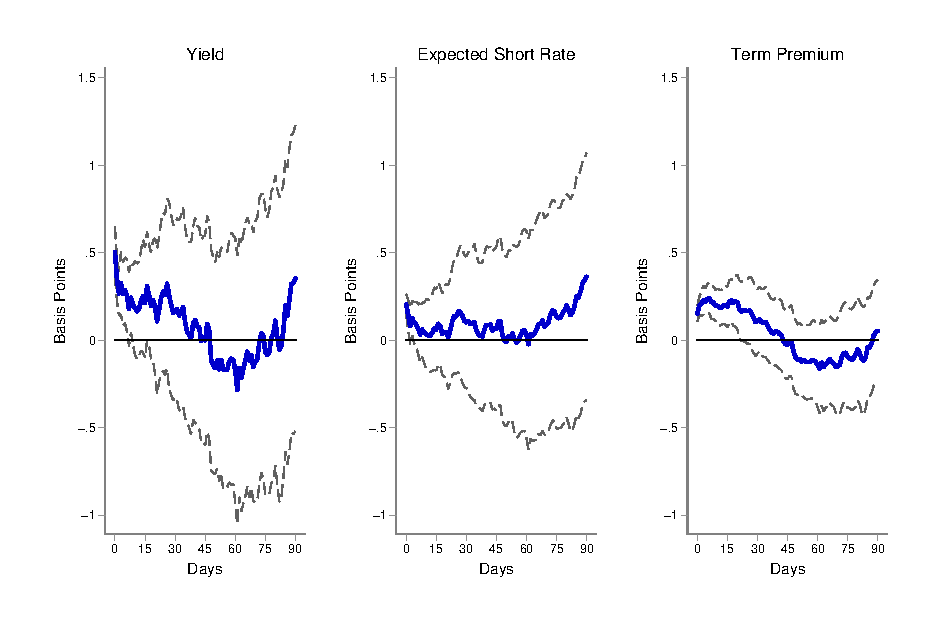
\includegraphics[trim={0cm 0cm 0cm 0cm},clip,height=0.24\textheight,width=\linewidth]{../Figures/LPs/LagDep-FX/Path/US/DCMP/PathUSDnomyptp24m.eps} \\
						\vspace{-0.35cm}
						\caption{Path Shock: 2000-2019} \label{subfig:LPUS2Ypath}
					\end{subfigure}
					
					\begin{subfigure}[t]{\linewidth}
						\includegraphics[trim={0cm 0cm 0cm 0cm},clip,height=0.24\textheight,width=\linewidth]{../Figures/LPs/LagDep-FX/LSAP/US/DCMP/LSAPUSDnomyptp24m.eps} \\
						\vspace{-0.35cm}
						\caption{LSAP Shock: 2009-2019} \label{subfig:LPUS2Ylsap}
					\end{subfigure}
				\end{center}
				\fignotes{This figure shows the response following \cite{Jorda:2005} of the 2-year U.S. yield and its components to U.S. monetary policy shocks. The U.S. yield is the zero coupon yield from \cite{GSW:2007}. The yield is decomposed into an expected future short-term interest rate and a term premium following \cite{KimWright:2005}. The target, path and LSAP shocks are identified using high-frequency data around Fed's monetary policy announcements, see section \ref{sec:USMPS} for details.}
			\end{minipage}
		\end{center}
	\end{figure}

	\pagebreak[4]
	
	\begin{figure}[tbph]
		\caption{Response of 10-Year U.S. Yield to U.S. Monetary Policy Shocks} \label{fig:LPUS10Y}
		\begin{center}
			\begin{minipage}{\linewidth}
				\begin{center}
					\begin{subfigure}[t]{\linewidth}
						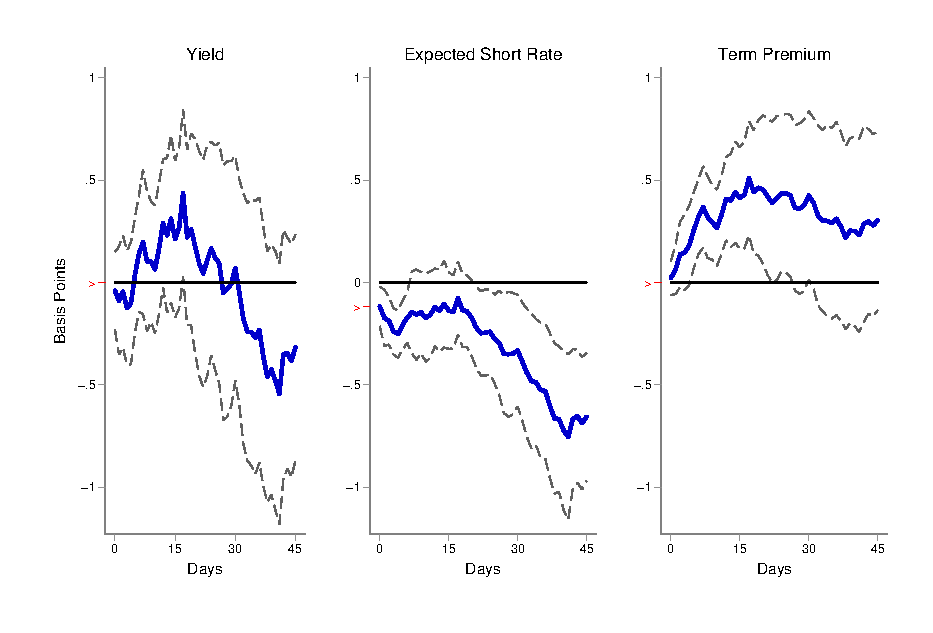
\includegraphics[trim={0cm 0cm 0cm 0cm},clip,height=0.24\textheight,width=\linewidth]{../Figures/LPs/LagDep-FX/Target/US/DCMP/TargetUSDnomyptp120m.eps} \\
						\vspace{-0.35cm}
						\caption{Target Shock: 2000-2008} \label{subfig:LPUS10Ytarget}
						\vspace{0.4cm}
					\end{subfigure}
					
					\begin{subfigure}[t]{\linewidth}
						\includegraphics[trim={0cm 0cm 0cm 0cm},clip,height=0.24\textheight,width=\linewidth]{../Figures/LPs/LagDep-FX/Path/US/DCMP/PathUSDnomyptp120m.eps} \\
						\vspace{-0.35cm}
						\caption{Path Shock: 2000-2019} \label{subfig:LPUS10Ypath}
					\end{subfigure}
					
					\begin{subfigure}[t]{\linewidth}
						\includegraphics[trim={0cm 0cm 0cm 0cm},clip,height=0.24\textheight,width=\linewidth]{../Figures/LPs/LagDep-FX/LSAP/US/DCMP/LSAPUSDnomyptp120m.eps} \\
						\vspace{-0.35cm}
						\caption{LSAP Shock: 2009-2019} \label{subfig:LPUS10Ylsap}
					\end{subfigure}
				\end{center}
				\fignotes{This figure shows the response following \cite{Jorda:2005} of the 10-year U.S. yield and its components to U.S. monetary policy shocks. The U.S. yield is the zero coupon yield from \cite{GSW:2007}. The yield is decomposed into an expected future short-term interest rate and a term premium following \cite{KimWright:2005}. The target, path and LSAP shocks are identified using high-frequency data around Fed's monetary policy announcements, see section \ref{sec:USMPS} for details.}
			\end{minipage}
		\end{center}
	\end{figure}
\end{document}
% trim = {<left> <lower> <right> <upper>}
\documentclass{article}
\usepackage{graphicx}
\usepackage[margin=1in]{geometry}
\usepackage[outdir=./]{epstopdf}  					% Avoids errors when input figures
\usepackage[labelsep=period,labelfont=bf]{caption}
%\usepackage{subcaption}

\begin{document}
	\begin{figure}[tbph]
		\caption{Response of 2-Year Emerging Market Yield to U.S. Monetary Policy Shocks} \label{fig:LPEM2Y}
		\begin{center}
			\begin{minipage}{\linewidth}
				\begin{center}
					\begin{subfigure}[t]{\linewidth}
						\includegraphics[trim={0cm 0cm 0cm 0cm},clip,height=0.24\textheight,width=\linewidth]{../Figures/LPs/LagDep-FX/Target/EM/TargetEMnomyptpphi24m.eps} \\
						\vspace{-0.35cm}
						\caption{Target Shock: 2000-2008} \label{subfig:LPEM2Ytarget}
						\vspace{0.4cm}
					\end{subfigure}
					
					\begin{subfigure}[t]{\linewidth}
						\includegraphics[trim={0cm 0cm 0cm 0cm},clip,height=0.24\textheight,width=\linewidth]{../Figures/LPs/LagDep-FX/Path/EM/PathEMnomyptpphi24m.eps} \\
						\vspace{-0.35cm}
						\caption{Path Shock: 2000-2019} \label{subfig:LPEM2Ypath}
					\end{subfigure}
					
					\begin{subfigure}[t]{\linewidth}
						\includegraphics[trim={0cm 0cm 0cm 0cm},clip,height=0.24\textheight,width=\linewidth]{../Figures/LPs/LagDep-FX/LSAP/EM/LSAPEMnomyptpphi24m.eps} \\
						\vspace{-0.35cm}
						\caption{LSAP Shock: 2009-2019} \label{subfig:LPEM2Ylsap}
					\end{subfigure}
				\end{center}
				\fignotes{This figure shows the response following \cite{Jorda:2005} of the 2-year emerging market nominal yield and its components to U.S. monetary policy shocks. The nominal yield is decomposed into an expected future short-term interest rate (ER), a term premium (TP) and a credit risk premium (CRP). The target, path and LSAP shocks are identified using high-frequency data around Fed's monetary policy announcements, see section \ref{sec:USMPS} for details.}
			\end{minipage}
		\end{center}
	\end{figure}
	
	\pagebreak[4]
	
	\begin{figure}[tbph]
		\caption{Response of 10-Year Emerging Market Yield to U.S. Monetary Policy Shocks} \label{fig:LPEM10Y}
		\begin{center}
			\begin{minipage}{\linewidth}
				\begin{center}
					\begin{subfigure}[t]{\linewidth}
						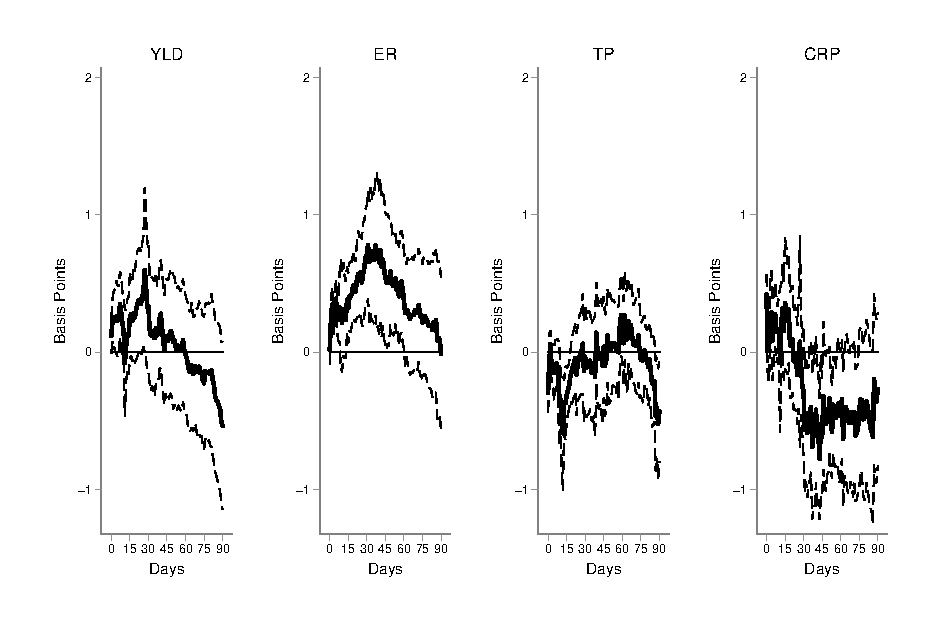
\includegraphics[trim={0cm 0cm 0cm 0cm},clip,height=0.24\textheight,width=\linewidth]{../Figures/LPs/LagDep-FX/Target/EM/TargetEMnomyptpphi120m.eps} \\
						\vspace{-0.35cm}
						\caption{Target Shock: 2000-2008} \label{subfig:LPEM10Ytarget}
						\vspace{0.4cm}
					\end{subfigure}
					
					\begin{subfigure}[t]{\linewidth}
						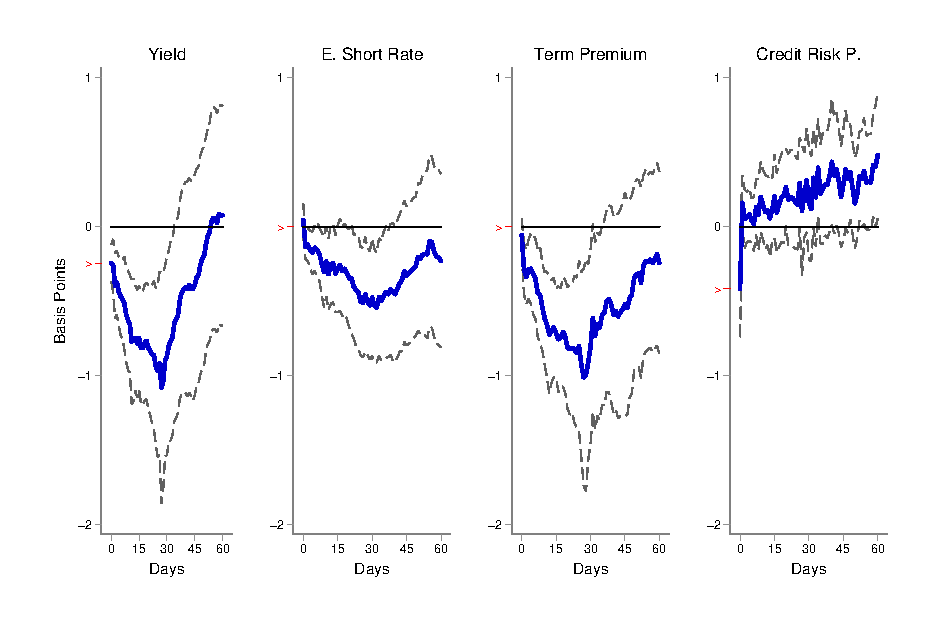
\includegraphics[trim={0cm 0cm 0cm 0cm},clip,height=0.24\textheight,width=\linewidth]{../Figures/LPs/LagDep-FX/Path/EM/PathEMnomyptpphi120m.eps} \\
						\vspace{-0.35cm}
						\caption{Path Shock: 2000-2019} \label{subfig:LPEM10Ypath}
					\end{subfigure}
					
					\begin{subfigure}[t]{\linewidth}
						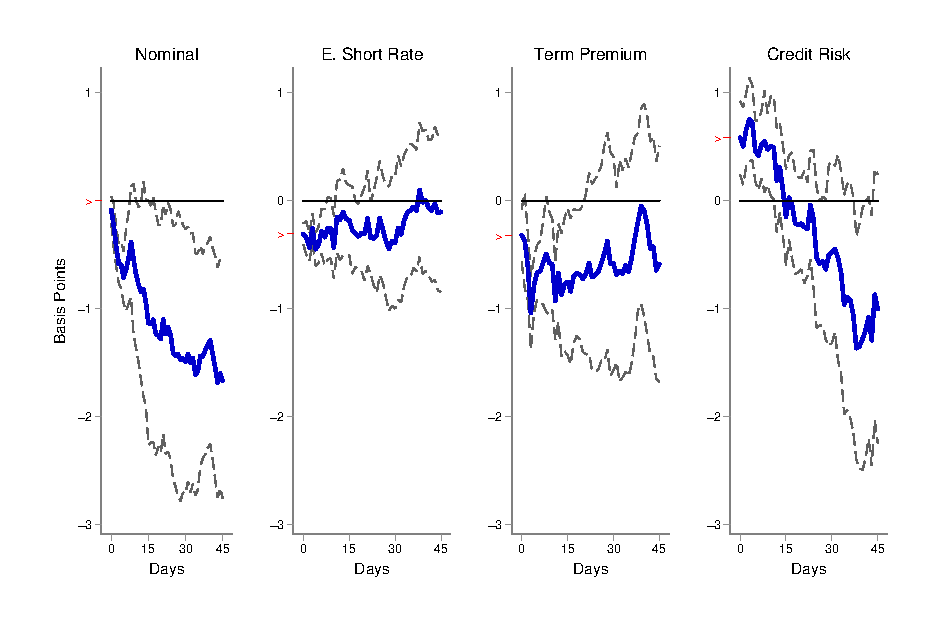
\includegraphics[trim={0cm 0cm 0cm 0cm},clip,height=0.24\textheight,width=\linewidth]{../Figures/LPs/LagDep-FX/LSAP/EM/LSAPEMnomyptpphi120m.eps} \\
						\vspace{-0.35cm}
						\caption{LSAP Shock: 2009-2019} \label{subfig:LPEM10Ylsap}
					\end{subfigure}
				\end{center}
				\fignotes{This figure shows the response following \cite{Jorda:2005} of the 10-year emerging market nominal yield and its components to U.S. monetary policy shocks. The nominal yield is decomposed into an expected future short-term interest rate (ER), a term premium (TP) and a credit risk premium (CRP). The target, path and LSAP shocks are identified using high-frequency data around Fed's monetary policy announcements, see section \ref{sec:USMPS} for details.}
			\end{minipage}
		\end{center}
	\end{figure}
\end{document}
% trim = {<left> <lower> <right> <upper>}
%\documentclass{article}
\usepackage{graphicx}
\usepackage[margin=1in]{geometry}
\usepackage[outdir=./]{epstopdf}  					% Avoids errors when input figures
\usepackage[labelsep=period,labelfont=bf]{caption}
%\usepackage{subcaption}

\begin{document}
	\begin{figure}[tbph]
		\caption{Response of 2-Year Advanced Country Yield to U.S. Monetary Policy Surprises} \label{fig:LPAE2Y}
		\begin{center}
			\begin{minipage}{\linewidth}
				\begin{center}
					\begin{subfigure}[t]{\linewidth}
						\includegraphics[trim={0cm 0cm 0cm 0cm},clip,height=0.24\textheight,width=\linewidth]{../Figures/LPs/LagDep-FX/Target/AE/TargetAEnomyptpphi24m.eps} \\
						\vspace{-0.35cm}
						\caption{Target Surprise: 2000-2008} \label{subfig:LPAE2Ytarget}
						\vspace{0.4cm}
					\end{subfigure}
					
					\begin{subfigure}[t]{\linewidth}
						\includegraphics[trim={0cm 0cm 0cm 0cm},clip,height=0.24\textheight,width=\linewidth]{../Figures/LPs/LagDep-FX/Path/AE/PathAEnomyptpphi24m.eps} \\
						\vspace{-0.35cm}
						\caption{Forward Guidance Surprise: 2000-2019} \label{subfig:LPAE2Ypath}
					\end{subfigure}
					
					\begin{subfigure}[t]{\linewidth}
						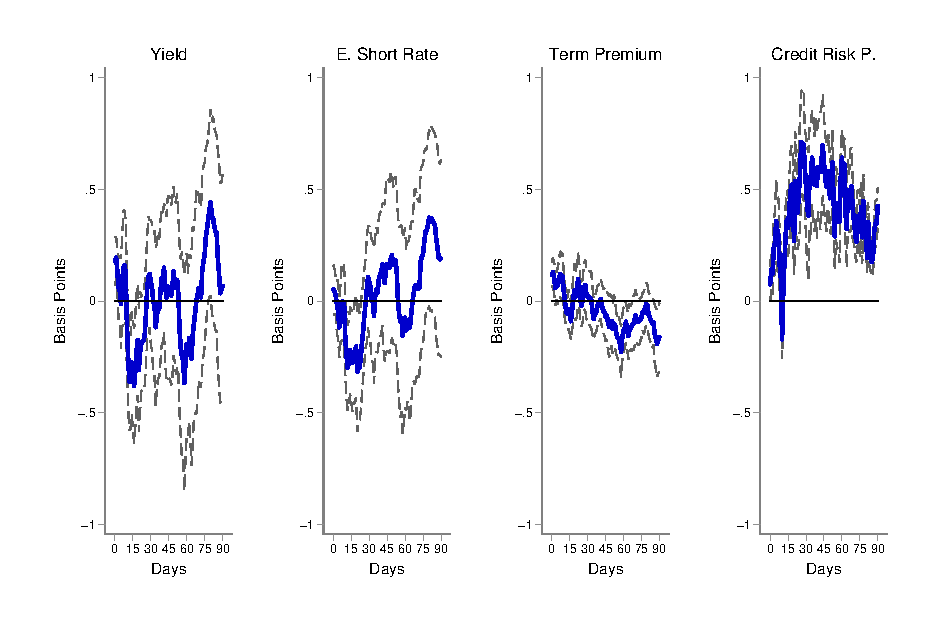
\includegraphics[trim={0cm 0cm 0cm 0cm},clip,height=0.24\textheight,width=\linewidth]{../Figures/LPs/LagDep-FX/LSAP/AE/LSAPAEnomyptpphi24m.eps} \\
						\vspace{-0.35cm}
						\caption{Asset Purchase Surprise: 2009-2019} \label{subfig:LPAE2Ylsap}
					\end{subfigure}
				\end{center}
				\fignotes{This figure shows the response following \cite{Jorda:2005} of the 2-year advanced country nominal yield and its components to U.S. monetary policy surprises. The nominal yield is decomposed into an expected future short-term interest rate (ER) and a term premium (TP). The target, forward guidance and asset purchase surprises are identified using high-frequency data around Fed's monetary policy announcements, see section \ref{sec:USMPS} for details.}
			\end{minipage}
		\end{center}
	\end{figure}
	
	\pagebreak[4]
	
	\begin{figure}[tbph]
		\caption{Response of 10-Year Advanced Country Yield to U.S. Monetary Policy Surprises} \label{fig:LPAE10Y}
		\begin{center}
			\begin{minipage}{\linewidth}
				\begin{center}
					\begin{subfigure}[t]{\linewidth}
						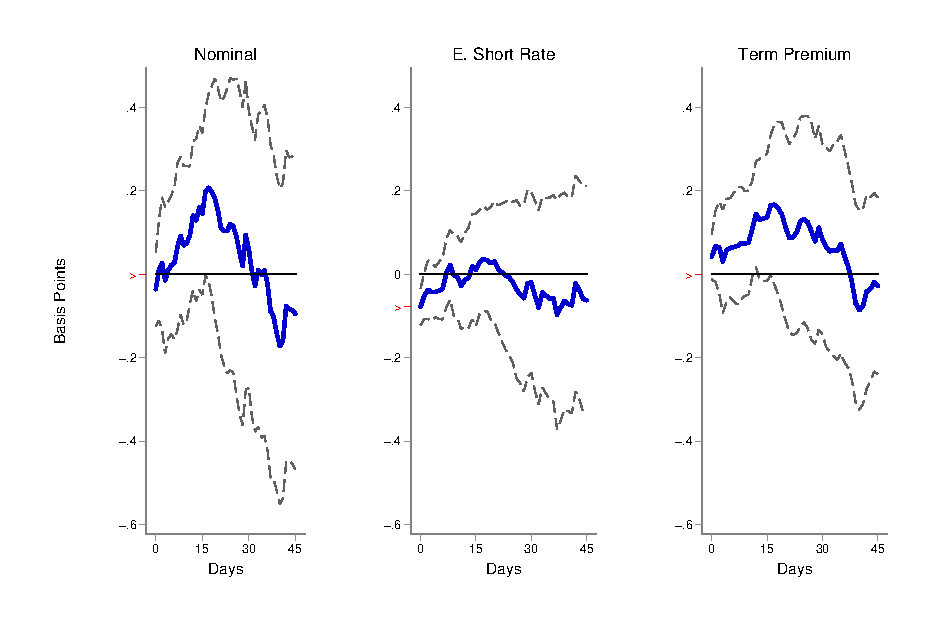
\includegraphics[trim={0cm 0cm 0cm 0cm},clip,height=0.24\textheight,width=\linewidth]{../Figures/LPs/LagDep-FX/Target/AE/TargetAEnomyptpphi120m.eps} \\
						\vspace{-0.35cm}
						\caption{Target Surprise: 2000-2008} \label{subfig:LPAE10Ytarget}
						\vspace{0.4cm}
					\end{subfigure}
					
					\begin{subfigure}[t]{\linewidth}
						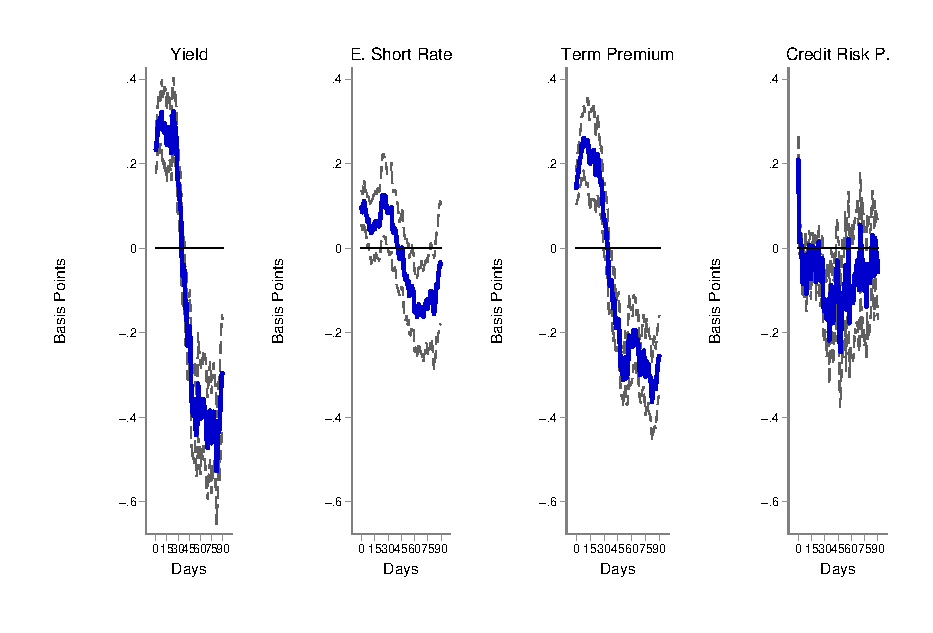
\includegraphics[trim={0cm 0cm 0cm 0cm},clip,height=0.24\textheight,width=\linewidth]{../Figures/LPs/LagDep-FX/Path/AE/PathAEnomyptpphi120m.eps} \\
						\vspace{-0.35cm}
						\caption{Forward Guidance Surprise: 2000-2019} \label{subfig:LPAE10Ypath}
					\end{subfigure}
					
					\begin{subfigure}[t]{\linewidth}
						\includegraphics[trim={0cm 0cm 0cm 0cm},clip,height=0.24\textheight,width=\linewidth]{../Figures/LPs/LagDep-FX/LSAP/AE/LSAPAEnomyptpphi120m.eps} \\
						\vspace{-0.35cm}
						\caption{Asset Purchase Surprise: 2009-2019} \label{subfig:LPAE10Ylsap}
					\end{subfigure}
				\end{center}
				\fignotes{This figure shows the response following \cite{Jorda:2005} of the 10-year advanced country nominal yield and its components to U.S. monetary policy surprises. The nominal yield is decomposed into an expected future short-term interest rate (ER) and a term premium (TP). The target, forward guidance and asset purchase surprises are identified using high-frequency data around Fed's monetary policy announcements, see section \ref{sec:USMPS} for details.}
			\end{minipage}
		\end{center}
	\end{figure}
\end{document}
% trim = {<left> <lower> <right> <upper>}
\documentclass{article}
\usepackage{graphicx}
\usepackage[margin=1in]{geometry}
\usepackage[outdir=./]{epstopdf}  					% Avoids errors when input figures
\usepackage[labelsep=period,labelfont=bf]{caption}
%\usepackage{subcaption}

\begin{document}

% trim = {<left> <lower> <right> <upper>}

\begin{figure}[tbph]
	\caption{Response of the Forward Premium to U.S. Monetary Policy Shocks: EM}
	\label{fig:LPEMRHO}
	\begin{subfigure}[t]{\textwidth}
		\begin{center}
			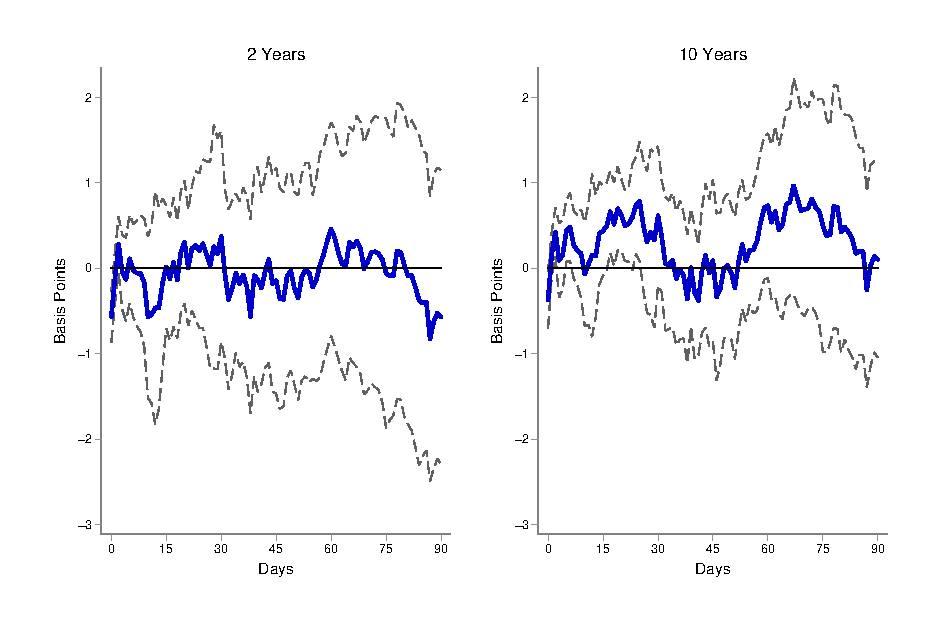
\includegraphics[trim={0cm 0cm 0cm 0cm},clip,height=0.26\textheight,width=1\textwidth]{../Figures/LPs/LagDep-FX/Target/EM/TargetEMrho.eps} \\
			\caption{Target Shock: 2000-2008} \label{subfig:LPEMRHOtarget}
%			\vspace{.5cm}
		\end{center}
	\end{subfigure}
	
	\begin{subfigure}[t]{\textwidth}
		\begin{center}
			\includegraphics[trim={0cm 0cm 0cm 0cm},clip,height=0.26\textheight,width=1\textwidth]{../Figures/LPs/LagDep-FX/Path/EM/PathEMrho.eps} \\
			\caption{Path Shock: 2000-2019} \label{subfig:LPEMRHOpath}
%			\vspace{.4cm}
		\end{center}
	\end{subfigure}
	
	\begin{subfigure}[t]{\textwidth}
		\begin{center}
			\includegraphics[trim={0cm 0cm 0cm 0cm},clip,height=0.26\textheight,width=1\textwidth]{../Figures/LPs/LagDep-FX/LSAP/EM/LSAPEMrho.eps} \\
			\caption{LSAP Shock: 2009-2019} \label{subfig:LPEMRHOlsap}
			%			\vspace{.4cm}
		\end{center}
	\end{subfigure}

%	\vspace{-0.4cm} \caption*{\footnotesize{\textit{Notes}: Notes.}}
\end{figure}

\pagebreak[4]

\begin{figure}[tbph]
	\caption{Response of the Forward Premium to U.S. Monetary Policy Shocks: AE}
	\label{fig:LPAERHO}
	\begin{subfigure}[t]{\textwidth}
		\begin{center}
			\includegraphics[trim={0cm 0cm 0cm 0cm},clip,height=0.26\textheight,width=1\textwidth]{../Figures/LPs/LagDep-FX/Target/AE/TargetAErho.eps} \\
			\caption{Target Shock: 2000-2008} \label{subfig:LPAERHOtarget}
			%			\vspace{.5cm}
		\end{center}
	\end{subfigure}
	
	\begin{subfigure}[t]{\textwidth}
		\begin{center}
			\includegraphics[trim={0cm 0cm 0cm 0cm},clip,height=0.26\textheight,width=1\textwidth]{../Figures/LPs/LagDep-FX/Path/AE/PathAErho.eps} \\
			\caption{Path Shock: 2000-2019} \label{subfig:LPAERHOpath}
			%			\vspace{.4cm}
		\end{center}
	\end{subfigure}
	
	\begin{subfigure}[t]{\textwidth}
		\begin{center}
			\includegraphics[trim={0cm 0cm 0cm 0cm},clip,height=0.26\textheight,width=1\textwidth]{../Figures/LPs/LagDep-FX/LSAP/AE/LSAPAErho.eps} \\
			\caption{LSAP Shock: 2009-2019} \label{subfig:LPAERHOlsap}
			%			\vspace{.4cm}
		\end{center}
	\end{subfigure}
	
	%	\vspace{-0.4cm} \caption*{\footnotesize{\textit{Notes}: Notes.}}
\end{figure}

\end{document}


\begin{landscape}
	\newpage
\end{landscape}

\iftoggle{fulldraft}{										% Turn it on/off in packages.tex
	\bibliographystyle{abbrvnat} 					% Other styles: {plain}, {authordate1}
	%\bibliography{../References/library}		% Uses local copy of database with references
	\bibliography{../../../References/library}	% Uses centralized database with references
	
	\newpage
\begin{appendices}
\iftoggle{toclinks}{\gototoc}{} % Turn it on/off in packages.tex, command in macros.tex
\iftoggle{cboxes}{	   				  % Turn it on/off in packages.tex
	\begin{boxeditems}
		\item Add link to website for Excel file with tickers.
		\item Add reference to paper that compares YC from Bloomberg for the Euro area.
	\end{boxeditems}}{}

\renewcommand\thefigure{\thesection.\arabic{figure}}
\section{Trend Inflation as a Proxy for Long-Term Inflation Forecasts} \label{sec:trendinf}
\setcounter{figure}{0}

An advantage of the small open economy approach is that it only requires forecasts for inflation, or a proxy in the case of countries with no long-term forecasts available as is the case for Israel and South Africa.

Inflation expectations are hoped to match measures of inflation that exclude unexpected shocks and better reflect the inflation environment.
Different measures of core inflation exist.
I use the inflation trend obtained by applying the Hodrick-Prescott filter to the series of realized inflation of each country.
Of course, the filter is sensitive to the sample period used.
The resulting trend can also be outside of the target inflation band due to the innate dynamics of the series, which would be at odds with survey data (see figure \ref{fig:wnCPI}).

%Fortunately, u
Unlike other countries, there is no marked upward or downward trend in the inflation of Israel nor South Africa during the sample period.
For each country, trend inflation is calculated for the whole period but only considered within the time range for which survey data is available for the rest of the countries, and as long as the trend is within the inflation target band.

Figure \ref{fig:CPI_ILSZAR} shows the realized and trend inflation for Israel and South Africa, and compares them with those of Malaysia and Thailand, two countries with a similar pattern for inflation (i.e. no marked trend) and for which survey data is available.
%It supports that t
Trend inflation seems to be a good proxy for the long-term inflation forecasts of Israel and South Africa.
Finally, since the 5-year and long-term forecasts closely follow each other (see figure \ref{fig:wnCPI}), I use trend inflation for both tenors.

\begin{landscape}
	\documentclass{article}
\usepackage{graphicx}
\usepackage[margin=1in]{geometry}
\usepackage[outdir=./]{epstopdf}  					% Avoids errors when input figures
\usepackage[labelsep=period,labelfont=bf]{caption}
%\usepackage{subcaption}

\begin{document}

\begin{figure}[tbph]
	\begin{center}
		\caption{Trend versus Long-Horizon Forecasts of Inflation}
		\label{fig:CPI_ILSZAR}
		\includegraphics[trim={0cm 0cm 0cm 0cm},clip,height=1\textheight,width=1.4\textwidth]{../Figures/Surveys/CPI_ILSZAR.eps} \\
	\end{center}
	% trim = {<left> <lower> <right> <upper>}
%	\vspace{-0.4cm} \caption*{\footnotesize{\textit{Notes}: Notes.}}
\end{figure}

\end{document}
\end{landscape}

%		\begin{figure}[!htbp]
		\begin{centering}
			\vspace{12.5mm}
			\includegraphics[width=1\textwidth,height=0.8\textheight]{../Figures/Temp/temp_ts_tp}
			\par\end{centering}
		\caption{Estimated Term Premia for Different Maturities.}\label{fig:temp_ts_tp}
	\end{figure}

\renewcommand\thefigure{\thesection.\arabic{figure}}
\section{Connectedness of Yield Components}
\setcounter{figure}{0}

%The expected short rate in emerging markets reacts to changes in the U.S. term premium. 
%This is consistent with the U.S. risk spillovers channel described by \cite{Kalemli-Ozcan:2019}.

%Here, I exploit it to provide new stylized facts about them that will help to interpret the results in the next section.
%To some extent, the response of emerging market yields to U.S. monetary policy shocks depends on 
%%how integrated are LC bonds to the global financial markets.
%%This requires to answer the question of 
%how connected are the sovereign yields of emerging markets.
%One way to address this question is to pool all yields together and see whether there is a global-level factor, associated with the first principal component.
%A global factor explains more than 90\% of the variation in the yields of advanced countries, 
%%consistent with \cite{DahlquistHasseltoft:2016}, 
%whereas it only explains around 50\% of the variation in the yields of emerging markets. % or their components.
%\footnote{ \cite{DuSchreger:2016JoF} find something similar for the credit risk compensation.}
%This suggests that the emerging market yields are not as connected among themselves as the yields of advanced countries.
%When yields are separated by maturity, a similar pattern emerges for the 1-year yields, whereas for the 10-year yields, a global factor explains around 95\% in AEs and 40\% in EMs. 
%Although a global factor plays a role in the variation of yields in both AEs and EMs, the bond yields in EMs are not as tightly connected as they are in AEs.
%These percentages are largely the same after the GFC.
%A global factor explains around 40\% of the variation of all the three components of yields in EMs.\footnote{ \cite{DuSchreger:2016JoF} also show that the credit risk compensation has a low reaction to global variables.} 
%For AEs, in contrast, a global factor explains 90\% of the variation in the expected short rate and 80\% in their term premia. 
%After the GFC, these percentages **increased** for the term premia in AEs and for the two components of the synthetic yields in EMs.

%A more formal way to analyze the comovement of %emerging market 
%%answer the question 
%yields is to measure the degree of connectedness among them.
%; that is, how much does the shock in one market has implications for the other markets.
%\cite{DieboldYilmaz:2014} propose a system-wide measure of connectedness 
%%based on forecast error variance decompositions.
%%Their methodology 
%that assesses shares of forecast error variation in a country's bond market due to shocks arising elsewhere.
%The connectedness index fluctuates between 0 and 100 percent, with higher numbers indicating a higher degree of comovement.
%Following \cite{ACDM:2019} and \cite{BostanciYilmaz:2020}, I obtain the connectedness index using a vector autoregression of order 1, with a forecast horizon of 10 days and a rolling window of 150 days for the daily changes of the 10-year nominal yield
%%of the emerging markets in the sample 
%and each of its components.

Figure \ref{fig:dyindex10y} shows that the connectedness index for the yields of emerging markets fluctuates around 30\%, %and advanced countries.
%\footnote{ The index for emerging markets has a shorter history because its computation requires a balanced panel. Also, since the construction of the synthetic curve does not involve nominal yields, the history of the components do not start on the same date.} 
%The index for emerging markets (figure \ref{subfig:dyindex10ydcmp}) captures some developments of the European sovereign debt crisis in 2012 and  the Greek debt crisis in 2015.
with notable spikes around the taper tantrum episode in 2013,
%\footnote{ During the episode, financial markets feared an earlier than expected withdrawal of the Fed's unconventional stimulus measures.} %and remained elevated for about a year.
%The second biggest spike %in the index occurred 
and after the 2016 U.S. presidential election.
%, with potential implications for some of the emerging markets in the sample.
%By mid-2017, the index was back to its pre-taper tantrum levels of around 30\% compared to an average value of the index for advanced countries of close to 70\%.
%The difference between the 
In contrast, \cite{ACDM:2019} report that the index fluctuates around 80\% for advanced countries.

The evidence of highly connected yields in advanced countries and low connected yields in emerging markets %might seem at odds with the idea of a 
%perspective based on the 
%global financial cycle \citep{Rey:2013}.
%On the one hand, the yields of advanced countries are highly connected among themselves (see figure \ref{subfig:dyindex10yAE}), which over the last decade has been driven by an increase in the connectedness of their term premia, as documented by \cite{ACDM:2019}.
%Changes in the compensation for risk in one advanced country not only spillover to other advanced countries but they have become increasingly important for the variation in their yields.
%On the other hand, the yields among emerging markets are not as connected as those in advanced countries (see figure \ref{subfig:dyindex10ydcmp}).
%The level of the index for emerging markets is about half the level of the index for advanced countries, it shows no upward trend for either their nominal yields or their components.\footnote{ \cite{ACDM:2019} already document that the increase in the connectedness of the yields of advanced countries has been driven by an increase in the connectedness of their term premia.}
% of emerging market yields do not show a clear trend, their relative importance seems to depend on the current economic environment.
%as might be expected under a perspective based on the global financial cycle. %according to the idea of the
%Is there a component that is more connected? 
%Unlike the rise in the connectedness of the term premium among advanced countries, 
%These results, however, are 
is consistent with a view %the global financial cycle 
in which global bond markets essentially operate under a core-periphery structure, in which the bond markets of advanced countries constitute the (highly interconnected) core and those of emerging markets represent the (less connected) periphery.
Countries in the periphery are in turn connected to the network mainly through countries in the core.\footnote{ The core-periphery structure has been shown to be a good description of different networks in economics and finance.} % \cite{CvP:2014} show, for example, that the interbank market operates under such a structure.
According to this view, shocks to emerging market yields are mainly idiosyncratic---reflected in less comovement---so
%figures \ref{subfig:dyindex10ydcmp} and \ref{subfig:dyindex10yAE} are measuring the connectedness of the periphery and the core, respectively.
%Therefore, 
what matters for them %emerging market yields 
are not spillovers originating in other emerging markets but in advanced countries.
%, which makes the argument of a global financial cycle stronger, not weaker.

The connectedness index for the yields of emerging markets shows no clear trend for either the nominal or synthetic yields nor their components. 
In contrast, \cite{ACDM:2019} document that the increase in the connectedness of the yields of advanced countries has been driven by an increase in the connectedness of their term premia.
Nevertheless, the term premia in emerging markets has been slightly more connected since 2013, whereas the credit risk compensation is relatively less connected (see figure \ref{subfig:dyindex10ydcmp}).
In fact, the level of the index for the synthetic yields tends to be higher than that for the nominal yields (see figure \ref{subfig:dyindex10ynomsyn}), suggesting that credit risk is indeed a more idiosyncratic component of the yields.

%Are the short and long end equally connected?
%Diebold-Yilmaz index for 2Y and 10Y to test Obsfeld vs K-O
%A related question is whether the connectedness of yields is the same throughout the term structure or whether some sections of the curves are more connected than others.
%%The role of a global factor seems to be different throughout the yield curve.
%\cite{Obstfeld:2015} 
%%shows that the effects of the global financial cycle are different at the short than at the long end of the yield curve. In particular, he 
%argues that long-term bonds are more globally connected than short term ones.
%On the other hand, \cite{Kalemli-Ozcan:2019} argues that short-term yields suffer more the effects of global influences.
%When yields are separated by maturity, a global factor explains around 50\% of the variation in the 1-year yields of EMs, compared to 90\% for AEs. 
%For the 10-year yields, a global factor explains around 60\% of the variability in EMs, relative to 95\% in AEs. 
%However, the role of the global factor is larger for the two components of the synthetic yield curve in the long end than for the short end.
%In sum, the role of a global component is larger for long-term yields and its components.
%Figure \ref{fig:dy_index_ts} plots the connectedness index for different maturities.
%It shows that the long end is relatively more connected than the short end, similar to what is observed for advanced countries, although this pattern became relevant for emerging markets after the taper tantrum episode.
%The figure also shows that the connectedness of the short end of the yield curves is similar between advanced and emerging markets.
%The difference in connectedness between the two groups of countries is therefore driven by the medium and long end of their yield curves.
%Although foreign participation in LC bond markets has increased, it is still mostly held by local investors, especially medium- and longer-term bonds as suggested by figure \ref{fig:dy_index_ts}, 
%%of emerging markets are far from being fully integrated in the global financial markets 
%and are therefore more responsive to local factors.
%In sum, while the yields of emerging markets are indeed globally connected, they are less so than the yields of advanced countries. 
%In particular, 
%Several factors can explain these patterns, including segmented markets, capital controls, home bias and regional differences.
%therefore seem to play a bigger role in the yields of EMs, and its components, than they do for AEs.

Finally, notice that the low connectedness among the yields of emerging markets supports estimating the term structure models for their yield curves separately (as it has been done in the paper) rather than jointly.

\documentclass{article}
\usepackage{graphicx}
\usepackage[margin=1in]{geometry}
\usepackage[outdir=./]{epstopdf}  					% Avoids errors when input figures
\usepackage[labelsep=period,labelfont=bf]{caption}
%\usepackage{subcaption}

\begin{document}
\begin{figure}[tbph]
\caption{Connectedness of Sovereign 10-Year Yields} \label{fig:dyindex10y}
\begin{center}
	\begin{minipage}{0.9\linewidth}
	\begin{center}
	\begin{subfigure}[t]{\linewidth}
			\includegraphics[trim={0cm 0cm 0cm 0cm},clip,height=0.34\textheight,width=\linewidth]{../Figures/Estimation/dy_index10y.eps} \\
			\vspace{-0.35cm}
			\caption{Emerging Markets} \label{subfig:dyindex10yEM}
			\vspace{0.4cm}
	\end{subfigure}
	
	\begin{subfigure}[t]{\linewidth}
			\includegraphics[trim={0cm 0cm 0cm 0cm},clip,height=0.34\textheight,width=\linewidth]{../Figures/Estimation/dy_index10y_AE.eps} \\
			\vspace{-0.35cm}
			\caption{Advanced Countries} \label{subfig:dyindex10yAE}
	\end{subfigure}
	\end{center}
	\fignotes{This figure plots the connected index of \cite{DieboldYilmaz:2014} for the 10-year nominal yields (solid line) of emerging markets and advanced countries. The figure also shows the index for each yield component. The yields of advanced countries are decomposed into an expected future short-term interest rate (line) and a term premium (line). The yields of emerging markets further have a credit risk premium (line). The index is obtained using a vector autoregression of order 1, with a forecast horizon of 10 days and a rolling window of 150 days for the daily changes of the 10-year nominal yields and each of their components. For emerging markets, the indexes have a shorter history because their computation requires a balanced panel; the indexes of the components do not start on the same date because the construction of the synthetic curves does not involve nominal yields.}
	\end{minipage}
\end{center}
\end{figure}
\end{document}
% trim = {<left> <lower> <right> <upper>} % appendix

%---------------------------------------------------------------
% Figures and Tables
%---------------------------------------------------------------
\renewcommand{\thetable}{\thesection.\arabic{table}}
\renewcommand\thefigure{\thesection.\arabic{figure}}
\section{Supplementary Tables} \label{sec:AppTables}
\setcounter{table}{0}

\documentclass[a4paper,12pt]{article}
\usepackage[labelsep=period,labelfont=bf]{caption}
\usepackage{multirow}
\usepackage{booktabs}
\usepackage{threeparttable}
\usepackage{pdflscape}
\usepackage{tabularx}
\usepackage[margin=1in]{geometry}
%% Personalized Macros
% Definitions, Equations, Table of Contents, Tables, Subcaptions, Paths, Text Fomats

%-------------------------------------------------------------------
% Variable Definitions
%-------------------------------------------------------------------
\providecommand{\tnr}{n}
\providecommand{\tnrfwd}{m}
\providecommand{\idxt}{t}
\providecommand{\idxi}{i}
\providecommand{\idxh}{h}
\providecommand{\idxs}{\idxt,\tnr}
\providecommand{\idxsfwd}{\tnr | \tnrfwd}
\providecommand{\idxsfwdt}{\idxt,\idxsfwd}
\providecommand{\idxspnl}{\idxi,\idxt}
\providecommand{\idxspnlfwd}{\idxi,{\idxt+\idxh}}
\providecommand{\idxspnllag}{\idxi,{\idxt-1}}
\providecommand{\idxspnllaglag}{\idxi,{\idxt-j}}
\providecommand{\fInst}{f_{\idxs}}
\providecommand{\yld}{y}
\providecommand{\xpc}{e}
\providecommand{\yZero}{\yld_{\idxs}}
\providecommand{\yZeroQ}{\yZero^{\Qmeasure}}
\providecommand{\yZeroP}{\yZero^{\Pmeasure}}
\providecommand{\yZeroE}{\yZero^{\xpc}}
\providecommand{\yZeroFwd}{\frate_{\idxsfwdt}}
\providecommand{\yZeroEfwd}{\yZeroFwd^{\xpc}}
\providecommand{\Pzero}{P_{\idxs}}
\providecommand{\Pzerolag}{P_{\idxt+1,\tnr-1}}
\providecommand{\srate}{i}
\providecommand{\shortrate}{\srate_{\idxt}}
\providecommand{\shortratelag}{\srate_{\idxt-1}}
\providecommand{\frate}{f}
\providecommand{\realrate}{r_{\idxs}}
\providecommand{\rateSvy}{\srate_{\idxs}^{survey}}
\providecommand{\SDF}{M_{\idxt+1}}
\providecommand{\SDFprod}{\ExpP \left[\Pi_{j=1} ^\tnr M_{\idxt+j}\right]}
\providecommand{\SDFsum}{\ExpQ \left[\exp \left(- \Sigma_{j=0} ^{\tnr-1} \srate_{\idxt+j} \right) \right]}
\providecommand{\Xvars}{X_{\idxt}}
\providecommand{\XvarsFwd}{X_{\idxt+1}}
\providecommand{\affineA}{A_{\tnr}}
\providecommand{\affineB}{B_{\tnr}}
\providecommand{\affineAfwd}{A_{\tnr + 1}}
\providecommand{\affineBfwd}{B_{\tnr + 1}}
\providecommand{\affineAQ}{\affineA^{\Qmeasure}}
\providecommand{\affineBQ}{\affineB^{\Qmeasure}}
\providecommand{\affineAP}{\affineA^{\Pmeasure}}
\providecommand{\affineBP}{\affineB^{\Pmeasure}}
\providecommand{\affineAe}{\affineA^{\xpc}}
\providecommand{\affineBe}{\affineB^{\xpc}}
\providecommand{\affineAeFwd}{A_{\idxsfwd}^{\xpc}}
\providecommand{\affineBeFwd}{B_{\idxsfwd}^{\xpc}}
\providecommand{\yLCnom}{\yld_{\idxs} ^{LC}}
\providecommand{\yLCsynt}{\widetilde{\yld}_{\idxs} ^{LC}}
\providecommand{\yUS}{y_{\idxs} ^{US}}
\providecommand{\yUSsynt}{\widetilde{\yld}_{\idxs} ^{US}}
\providecommand{\fx}{\mathit{s}}

% Math fonts
\providecommand{\Xdim}{\mathrm{K}}
\providecommand{\Ydim}{\mathrm{N}}
\providecommand{\Sdim}{\mathrm{S}}
\providecommand{\Normal}{\mathcal{N}}
\providecommand{\Pmeasure}{\mathbb{P}}
\providecommand{\Qmeasure}{\mathbb{Q}}
\providecommand{\Expec}{\mathrm{E}_{t}}
\providecommand{\ExpP}{\mathrm{E}^{\Pmeasure}_{t}}
\providecommand{\ExpQ}{\mathrm{E}^{\Qmeasure}_{t}}
\providecommand{\Svy}{S}
\providecommand{\yVec}{\mathbf{\yld}_{t}}
\providecommand{\ySVec}{\yVec^{\Svy}}
\providecommand{\Avec}{\mathbf{A}}
\providecommand{\Bvec}{\mathbf{B}}
\providecommand{\ASvec}{\mathbf{A}^{\Svy}}
\providecommand{\BSvec}{\mathbf{B}^{\Svy}}
\providecommand{\uVec}{\mathbf{u}_{t}}
\providecommand{\uSVec}{\mathbf{u}_{t}^{\Svy}}
\providecommand{\Svec}{\mathbf{\Sigma}}
\providecommand{\SyVec}{\mathbf{\Svec}_{Y}}
\providecommand{\SsVec}{\mathbf{\Svec}_{\Svy}}

% Greeks
\providecommand{\termprm}{\tau_{\idxs}}
\providecommand{\riskprice}{\lambda_{t}}
\providecommand{\lambdazero}{\lambda_{0}}
\providecommand{\lambdaone}{\lambda_{1}}
\providecommand{\fwdprm}{\rho_{\idxs}}
\providecommand{\CIPdev}{\phi_{\idxs}}
\providecommand{\deltazero}{\delta_{0}}
\providecommand{\deltaone}{\delta_{1}}
\providecommand{\error}{\nu_{t+1}}
\providecommand{\errorQ}{\error^{\Qmeasure}}
\providecommand{\errorP}{\error^{\Pmeasure}}
\providecommand{\XmuP}{\mu^{\Pmeasure}}
\providecommand{\XmuQ}{\mu^{\Qmeasure}}
\providecommand{\XSigma}{\Sigma}
\providecommand{\XPhiP}{\Phi^{\Pmeasure}}
\providecommand{\XPhiQ}{\Phi^{\Qmeasure}}
\providecommand{\betaLT}{\beta_{0}}
\providecommand{\betaST}{\beta_{1}}
\providecommand{\betaMTns}{\beta_{2}}
\providecommand{\betaMTnss}{\beta_{3}}
\providecommand{\tauNS}{\tau_{1}}
\providecommand{\tauNSS}{\tau_{2}}
\providecommand{\tnrTauNS}{\tnr/\tauNS}
\providecommand{\tnrTauNSS}{\tnr/\tauNSS}
\providecommand{\params}{\theta}
\providecommand{\Vasy}{\Omega}
\providecommand{\cmpnt}{\Psi}
\providecommand{\Jacobian}{\Gamma}
\providecommand{\Hessian}{\mathcal{H}_\params}
\providecommand{\asydstr}{\sqrt{\Ydim} \left( \widehat{\cmpnt} - \cmpnt \right) \xrightarrow[]{d} \Normal \left(0,\, \Jacobian \, \Vasy \, \Jacobian' \right)}
\providecommand{\sampleHjoint}{\frac{1}{\Ydim} \frac{\partial^{2} \ell_{\Ydim} (\widehat{\params})}{\partial \params \partial \params'}}
\providecommand{\sampleHindiv}{\frac{1}{\Ydim} \sum_{i = 1}^{\Ydim} \frac{\partial^{2} \log \mathit{f} (X_{i} | \widehat{\params})}{\partial \params \partial \params'}}

% Nelson-Siegel_Svensson
\providecommand{\loadSTnsFwd}{\exp\left(-\tnrTauNS \right)}
\providecommand{\loadSTnssFwd}{\exp\left(-\tnrTauNSS \right)}
\providecommand{\loadMTnsFwd}{\left(\tnrTauNS\right) \loadSTnsFwd}
\providecommand{\loadMTnssFwd}{\left(\tnrTauNSS\right) \loadSTnssFwd}
\providecommand{\loadSTnsZero}{\frac{1-\loadSTnsFwd}{\tnrTauNS}}
\providecommand{\loadSTnssZero}{\frac{1-\loadSTnssFwd}{\tnrTauNSS}}
\providecommand{\loadMTnsZero}{\left(\loadSTnsZero - \loadSTnsFwd \right)}
\providecommand{\loadMTnssZero}{\left( \loadSTnssZero - \loadSTnssFwd \right)}

%\providecommand{\}{}
% DELETE in a later revision
\providecommand{\Xmu}{\mu}
\providecommand{\XPhi}{\Phi}
\providecommand{\XmuStar}{\mu^{*}}
\providecommand{\XPhiStar}{\Phi^{*}}
\providecommand{\STrate}{r}
\providecommand{\rShort}{\STrate_{t}}
\providecommand{\rShortlag}{\STrate_{t-1}}
\providecommand{\ySvy}{\STrate_{\idxs}^{survey}}
\providecommand{\TPatsm}{tp_{\idxs}}

%-------------------------------------------------------------------
% Equations
%-------------------------------------------------------------------
\newcommand{\eqyLCsynt}{\yLCsynt = \yUS + \fwdprm}
\newcommand{\eqCIPdevDS}{\CIPdev = \yLCnom - \yLCsynt}
\newcommand{\eqCIPdevQ}{\CIPdev = \yLCnom - \yZeroQ}

\newcommand{\PzeroP}{\Pzero = \ExpP \left[ \SDF \Pzerolag \right]}
\newcommand{\PzeroQ}{\Pzero = \ExpQ \left[ \exp\left(- \shortrate\right) \Pzerolag \right]}

\newcommand{\eqXvarsFwdQ}{\XvarsFwd = \XmuQ + \XPhiQ \Xvars  + \XSigma \errorQ}
\newcommand{\eqshortrate}{\shortrate = \deltazero + \deltaone' \Xvars}
\newcommand{\eqyZeroP}{\yZeroP = \affineAP + \affineBP \Xvars}
\newcommand{\eqyZeroQ}{\yZeroQ = \affineAQ + \affineBQ \Xvars}
\newcommand{\eqTP}{\termprm = \yZeroQ - \yZeroP}
\newcommand{\eqXvarsFwdP}{\XvarsFwd = \XmuP + \XPhiP \Xvars  + \XSigma \errorP}
\newcommand{\eqriskprice}{\riskprice = \lambdazero + \lambdaone \Xvars}
\newcommand{\eqSDF}{\SDF = \exp\left( -\shortrate -\frac{1}{2} \riskprice' \riskprice - \riskprice' \errorP \right)}
%\newcommand{}{}

\newcommand{\eqpanelUCSV}{\tau_{\idxspnl} = \alpha_{\idxi} + \beta_{1} \sigma^{\pi}_{\idxspnl} + \beta_{2} g_{\idxspnl} + u_{\idxspnl}}
\newcommand{\eqpanelTPreg}{\yld_{\idxspnl} = \alpha_{\idxi} + \gamma_{1}' z^{1}_{\idxspnl} + \gamma_{2}' z^{2}_{\idxspnl} + u_{\idxspnl}}
\newcommand{\eqySvy}{\rateSvy = \frac{\widehat{\beta}_{0}}{1-\widehat{\beta}_{\srate}} + \frac{\widehat{\beta}_{{\pi}}}{1-\widehat{\beta}_{\srate}} \pi_{\idxs}^{survey} + \frac{\widehat{\beta}_{{g}}}{1-\widehat{\beta}_{\srate}} g_{\idxs}^{survey} }

\newcommand{\eqyFwd}{\yZeroFwd = \left( \tnrfwd \yld_{\idxt,\tnrfwd} - \tnr \yZero \right)/ \left( \tnrfwd - \tnr \right) }
\newcommand{\eqAeFwd}{\affineAeFwd = \left( \tnrfwd A_{\tnrfwd}^{\xpc}  - \tnr \affineAe \right)/ \left( \tnrfwd - \tnr \right) }
\newcommand{\eqBeFwd}{\affineAeFwd = \left( \tnrfwd B_{\tnrfwd}^{\xpc}  - \tnr \affineBe \right)/ \left( \tnrfwd - \tnr \right) }
\newcommand{\eqrrt}{\rateSvy = \pi^{CE survey}_{\idxs} + \realrate^{*} = \pi^{CE survey}_{\idxs} + \left( \srate^{SPF survey}_{\idxs} - \pi^{SPF survey}_{\idxs} \right) }


\newcommand{\eqyVecY}{\yVec = \Avec + \Bvec \Xvars + \SyVec \uVec}
\newcommand{\eqyVecS}{\ySVec = \ASvec + \BSvec \Xvars + \SsVec \uSVec}

% One shock at a time
%\newcommand{\eqpanelLP}{\yld_{\idxspnlfwd} - \yld_{\idxspnllag} = \alpha_{\idxh,\idxi} + \beta_{\idxh} \epsilon_{\idxt} + \gamma_{\idxh} \Delta \yld_{\idxspnllag} + \phi_{\idxh} \fx_{\idxspnllag}  + u_{\idxspnlfwd}}

% All shocks at once
\newcommand{\eqpanelLP}{\yld_{\idxspnlfwd} - \yld_{\idxspnllag} = \alpha_{\idxh,\idxi} + \sum^{3}_{j = 1} \beta^{j}_{\idxh} \epsilon^{j}_{\idxt} + \gamma_{\idxh} \Delta \yld_{\idxspnllag} + \eta_{\idxh} \fx_{\idxspnllag}  + u_{\idxspnlfwd}} 

\newcommand{\eqpanelLPlevels}{\yld_{\idxspnlfwd} = \alpha_{\idxh,\idxi} + \sum^{3}_{j = 1} \beta^{j}_{\idxh} \epsilon^{j}_{\idxt} + \sum^{2}_{j = 1} \gamma^{j}_{\idxh} \yld_{\idxspnllaglag} + \eta_{\idxh} \fx_{\idxspnllag}  + u_{\idxspnlfwd}} 
% \beta^{target}_{\idxh} \epsilon^{target}_{\idxt} + \beta^{path}_{\idxh} \epsilon^{path}_{\idxt} + \beta^{lsap}_{\idxh} \epsilon^{lsap}_{\idxt} 

%---------------------------------------------------------------
% Table of Contents
%---------------------------------------------------------------
% Link to ToC from section
\newcommand{\gototoc}{\vspace{-2cm} \null\hfill [\hyperlink{toc}{Go2ToC}] \newline}

% Link back to section from ToC
\newcommand{\maketoc}{
	\hypertarget{toc}{}
	\newpage
	\tableofcontents
	\vspace{2.5\bigskipamount} }

% Box with bullets for tasks to do in a section
\newenvironment{boxeditems}
	{\begin{tabular}{|p{\linewidth}|}
	\hline
	\begin{itemize}
	}
	{
	\end{itemize}
	\\ \hline
	\end{tabular} \\
	}

%---------------------------------------------------------------
% Tables: Estout Commands following Jörg Weber
%---------------------------------------------------------------
\newcommand{\sym}[1]{\rlap{#1}}

\let\estinput=\input	% define new input command to flatten the document

\newcommand{\estauto}[2]{
	\newcolumntype{C}{>{\centering\arraybackslash}X}
	\vspace{.75ex}{
%		\begin{tabularx}{1.4\textwidth}{l*{#2}C}
		\begin{tabularx}{0.95\linewidth}{l*{#2}C}
			\toprule
			\estinput{#1}
			\\ \bottomrule
			\addlinespace[.75ex]
		\end{tabularx}
	}
}

% Allow line breaks with \\ in specialcells
\newcommand{\specialcell}[2][c]{\begin{tabular}[#1]{@{}c@{}}#2\end{tabular}}

%---------------------------------------------------------------
% Subcaptions
%---------------------------------------------------------------
% Notes after figures following Jörg Weber
\newcommand{\figtext}[1]{
	\vspace{-1ex}
	\captionsetup{justification=justified,font=footnotesize}
	\caption*{#1}
%	\captionsetup{justification=raggedright,singlelinecheck=false,font=footnotesize}
%	\caption*{\hspace{6pt}\hangindent=1.5em #1}
}

\newcommand{\fignote}[1]{\figtext{\emph{Note:~}~#1}}
\newcommand{\fignotes}[1]{\figtext{\emph{Notes:~}~#1}}

% Notes after tables
\newcommand{\tabnote}[1]{
	\begin{tablenotes}[para,flushleft]
		\footnotesize \emph{Notes:~}~#1
	\end{tablenotes}
}

%---------------------------------------------------------------
% Paths
%---------------------------------------------------------------
%\newcommand*{\pathFigs}{../Figures}
%\input{pathFigs/fig1.tex}

%---------------------------------------------------------------
% Text Fomats
%---------------------------------------------------------------
%\newcommand{\txtbi}[1]{\textbf{\textit{#1}}}

%---------------------------------------------------------------
% Other
%---------------------------------------------------------------
%\newcommand\LL[1]{\multicolumn{2}{|l}{#1}}
%\newcommand\RR[1]{\multicolumn{2}{c|}{#1}}
%\newcommand\LR[1]{\multicolumn{2}{|c|}{#1}}
%\newcommand\LL[1]{\multicolumn{1}{|c}{#1}}
%\newcommand\RR[1]{\multicolumn{1}{c|}{#1}}
%\newcommand\LR[1]{\multicolumn{1}{|c|}{#1}}
\pagestyle{empty}

\begin{document}
	\begin{normalsize}
%		\begin{landscape}
			\begin{table}[!h]
				\begin{center}
					\caption{Drivers of the Emerging Market 5-Year Nominal Yield and Its Components} \label{tab:ycdcmp5y}
					\begin{threeparttable}
						\estauto{../Tables/f_ycdcmp5y.tex}{6}
						\tabnote{This table reports the estimated slope coefficients of panel data regressions of the 5-year nominal yield and its components (expected short rate, term premium and credit risk compensation) on selected explanatory variables. The sample includes monthly data for 15 emerging markets starting in 2000:1 and ending in 2019:1. The dependent variables are expressed in basis points. The explanatory variables are the U.S. term premium and the U.S. expected short rate according to \cite{KimWright:2005}  with the same maturity as the dependent variables, the policy rate, domestic inflation and unemployment, the standardized exchange rate (local currency per USD), the log of the Vix, the log of the U.S. and global economic policy uncertainty indexes based on \cite{BakerBloomDavis:2016}, the global economic activity index of \cite{Hamilton:2019}. Driscoll--Kraay standard errors in parenthesis; lag length up to which the residuals may be autocorrelated is indicated. *, **, *** asterisks respectively indicate significance at the 10\%, 5\% and 1\% level.}
					\end{threeparttable}
				\end{center}
			\end{table}
%		\end{landscape}
	\end{normalsize}
\end{document} % appendix
\documentclass[a4paper,12pt]{article}
\usepackage[labelsep=period,labelfont=bf]{caption}
\usepackage{multirow}
\usepackage{booktabs}
\usepackage{threeparttable}
\usepackage{pdflscape}
\usepackage{tabularx}
\usepackage[margin=1in]{geometry}
%% Personalized Macros
% Definitions, Equations, Table of Contents, Tables, Subcaptions, Paths, Text Fomats

%-------------------------------------------------------------------
% Variable Definitions
%-------------------------------------------------------------------
\providecommand{\tnr}{n}
\providecommand{\tnrfwd}{m}
\providecommand{\idxt}{t}
\providecommand{\idxi}{i}
\providecommand{\idxh}{h}
\providecommand{\idxs}{\idxt,\tnr}
\providecommand{\idxsfwd}{\tnr | \tnrfwd}
\providecommand{\idxsfwdt}{\idxt,\idxsfwd}
\providecommand{\idxspnl}{\idxi,\idxt}
\providecommand{\idxspnlfwd}{\idxi,{\idxt+\idxh}}
\providecommand{\idxspnllag}{\idxi,{\idxt-1}}
\providecommand{\idxspnllaglag}{\idxi,{\idxt-j}}
\providecommand{\fInst}{f_{\idxs}}
\providecommand{\yld}{y}
\providecommand{\xpc}{e}
\providecommand{\yZero}{\yld_{\idxs}}
\providecommand{\yZeroQ}{\yZero^{\Qmeasure}}
\providecommand{\yZeroP}{\yZero^{\Pmeasure}}
\providecommand{\yZeroE}{\yZero^{\xpc}}
\providecommand{\yZeroFwd}{\frate_{\idxsfwdt}}
\providecommand{\yZeroEfwd}{\yZeroFwd^{\xpc}}
\providecommand{\Pzero}{P_{\idxs}}
\providecommand{\Pzerolag}{P_{\idxt+1,\tnr-1}}
\providecommand{\srate}{i}
\providecommand{\shortrate}{\srate_{\idxt}}
\providecommand{\shortratelag}{\srate_{\idxt-1}}
\providecommand{\frate}{f}
\providecommand{\realrate}{r_{\idxs}}
\providecommand{\rateSvy}{\srate_{\idxs}^{survey}}
\providecommand{\SDF}{M_{\idxt+1}}
\providecommand{\SDFprod}{\ExpP \left[\Pi_{j=1} ^\tnr M_{\idxt+j}\right]}
\providecommand{\SDFsum}{\ExpQ \left[\exp \left(- \Sigma_{j=0} ^{\tnr-1} \srate_{\idxt+j} \right) \right]}
\providecommand{\Xvars}{X_{\idxt}}
\providecommand{\XvarsFwd}{X_{\idxt+1}}
\providecommand{\affineA}{A_{\tnr}}
\providecommand{\affineB}{B_{\tnr}}
\providecommand{\affineAfwd}{A_{\tnr + 1}}
\providecommand{\affineBfwd}{B_{\tnr + 1}}
\providecommand{\affineAQ}{\affineA^{\Qmeasure}}
\providecommand{\affineBQ}{\affineB^{\Qmeasure}}
\providecommand{\affineAP}{\affineA^{\Pmeasure}}
\providecommand{\affineBP}{\affineB^{\Pmeasure}}
\providecommand{\affineAe}{\affineA^{\xpc}}
\providecommand{\affineBe}{\affineB^{\xpc}}
\providecommand{\affineAeFwd}{A_{\idxsfwd}^{\xpc}}
\providecommand{\affineBeFwd}{B_{\idxsfwd}^{\xpc}}
\providecommand{\yLCnom}{\yld_{\idxs} ^{LC}}
\providecommand{\yLCsynt}{\widetilde{\yld}_{\idxs} ^{LC}}
\providecommand{\yUS}{y_{\idxs} ^{US}}
\providecommand{\yUSsynt}{\widetilde{\yld}_{\idxs} ^{US}}
\providecommand{\fx}{\mathit{s}}

% Math fonts
\providecommand{\Xdim}{\mathrm{K}}
\providecommand{\Ydim}{\mathrm{N}}
\providecommand{\Sdim}{\mathrm{S}}
\providecommand{\Normal}{\mathcal{N}}
\providecommand{\Pmeasure}{\mathbb{P}}
\providecommand{\Qmeasure}{\mathbb{Q}}
\providecommand{\Expec}{\mathrm{E}_{t}}
\providecommand{\ExpP}{\mathrm{E}^{\Pmeasure}_{t}}
\providecommand{\ExpQ}{\mathrm{E}^{\Qmeasure}_{t}}
\providecommand{\Svy}{S}
\providecommand{\yVec}{\mathbf{\yld}_{t}}
\providecommand{\ySVec}{\yVec^{\Svy}}
\providecommand{\Avec}{\mathbf{A}}
\providecommand{\Bvec}{\mathbf{B}}
\providecommand{\ASvec}{\mathbf{A}^{\Svy}}
\providecommand{\BSvec}{\mathbf{B}^{\Svy}}
\providecommand{\uVec}{\mathbf{u}_{t}}
\providecommand{\uSVec}{\mathbf{u}_{t}^{\Svy}}
\providecommand{\Svec}{\mathbf{\Sigma}}
\providecommand{\SyVec}{\mathbf{\Svec}_{Y}}
\providecommand{\SsVec}{\mathbf{\Svec}_{\Svy}}

% Greeks
\providecommand{\termprm}{\tau_{\idxs}}
\providecommand{\riskprice}{\lambda_{t}}
\providecommand{\lambdazero}{\lambda_{0}}
\providecommand{\lambdaone}{\lambda_{1}}
\providecommand{\fwdprm}{\rho_{\idxs}}
\providecommand{\CIPdev}{\phi_{\idxs}}
\providecommand{\deltazero}{\delta_{0}}
\providecommand{\deltaone}{\delta_{1}}
\providecommand{\error}{\nu_{t+1}}
\providecommand{\errorQ}{\error^{\Qmeasure}}
\providecommand{\errorP}{\error^{\Pmeasure}}
\providecommand{\XmuP}{\mu^{\Pmeasure}}
\providecommand{\XmuQ}{\mu^{\Qmeasure}}
\providecommand{\XSigma}{\Sigma}
\providecommand{\XPhiP}{\Phi^{\Pmeasure}}
\providecommand{\XPhiQ}{\Phi^{\Qmeasure}}
\providecommand{\betaLT}{\beta_{0}}
\providecommand{\betaST}{\beta_{1}}
\providecommand{\betaMTns}{\beta_{2}}
\providecommand{\betaMTnss}{\beta_{3}}
\providecommand{\tauNS}{\tau_{1}}
\providecommand{\tauNSS}{\tau_{2}}
\providecommand{\tnrTauNS}{\tnr/\tauNS}
\providecommand{\tnrTauNSS}{\tnr/\tauNSS}
\providecommand{\params}{\theta}
\providecommand{\Vasy}{\Omega}
\providecommand{\cmpnt}{\Psi}
\providecommand{\Jacobian}{\Gamma}
\providecommand{\Hessian}{\mathcal{H}_\params}
\providecommand{\asydstr}{\sqrt{\Ydim} \left( \widehat{\cmpnt} - \cmpnt \right) \xrightarrow[]{d} \Normal \left(0,\, \Jacobian \, \Vasy \, \Jacobian' \right)}
\providecommand{\sampleHjoint}{\frac{1}{\Ydim} \frac{\partial^{2} \ell_{\Ydim} (\widehat{\params})}{\partial \params \partial \params'}}
\providecommand{\sampleHindiv}{\frac{1}{\Ydim} \sum_{i = 1}^{\Ydim} \frac{\partial^{2} \log \mathit{f} (X_{i} | \widehat{\params})}{\partial \params \partial \params'}}

% Nelson-Siegel_Svensson
\providecommand{\loadSTnsFwd}{\exp\left(-\tnrTauNS \right)}
\providecommand{\loadSTnssFwd}{\exp\left(-\tnrTauNSS \right)}
\providecommand{\loadMTnsFwd}{\left(\tnrTauNS\right) \loadSTnsFwd}
\providecommand{\loadMTnssFwd}{\left(\tnrTauNSS\right) \loadSTnssFwd}
\providecommand{\loadSTnsZero}{\frac{1-\loadSTnsFwd}{\tnrTauNS}}
\providecommand{\loadSTnssZero}{\frac{1-\loadSTnssFwd}{\tnrTauNSS}}
\providecommand{\loadMTnsZero}{\left(\loadSTnsZero - \loadSTnsFwd \right)}
\providecommand{\loadMTnssZero}{\left( \loadSTnssZero - \loadSTnssFwd \right)}

%\providecommand{\}{}
% DELETE in a later revision
\providecommand{\Xmu}{\mu}
\providecommand{\XPhi}{\Phi}
\providecommand{\XmuStar}{\mu^{*}}
\providecommand{\XPhiStar}{\Phi^{*}}
\providecommand{\STrate}{r}
\providecommand{\rShort}{\STrate_{t}}
\providecommand{\rShortlag}{\STrate_{t-1}}
\providecommand{\ySvy}{\STrate_{\idxs}^{survey}}
\providecommand{\TPatsm}{tp_{\idxs}}

%-------------------------------------------------------------------
% Equations
%-------------------------------------------------------------------
\newcommand{\eqyLCsynt}{\yLCsynt = \yUS + \fwdprm}
\newcommand{\eqCIPdevDS}{\CIPdev = \yLCnom - \yLCsynt}
\newcommand{\eqCIPdevQ}{\CIPdev = \yLCnom - \yZeroQ}

\newcommand{\PzeroP}{\Pzero = \ExpP \left[ \SDF \Pzerolag \right]}
\newcommand{\PzeroQ}{\Pzero = \ExpQ \left[ \exp\left(- \shortrate\right) \Pzerolag \right]}

\newcommand{\eqXvarsFwdQ}{\XvarsFwd = \XmuQ + \XPhiQ \Xvars  + \XSigma \errorQ}
\newcommand{\eqshortrate}{\shortrate = \deltazero + \deltaone' \Xvars}
\newcommand{\eqyZeroP}{\yZeroP = \affineAP + \affineBP \Xvars}
\newcommand{\eqyZeroQ}{\yZeroQ = \affineAQ + \affineBQ \Xvars}
\newcommand{\eqTP}{\termprm = \yZeroQ - \yZeroP}
\newcommand{\eqXvarsFwdP}{\XvarsFwd = \XmuP + \XPhiP \Xvars  + \XSigma \errorP}
\newcommand{\eqriskprice}{\riskprice = \lambdazero + \lambdaone \Xvars}
\newcommand{\eqSDF}{\SDF = \exp\left( -\shortrate -\frac{1}{2} \riskprice' \riskprice - \riskprice' \errorP \right)}
%\newcommand{}{}

\newcommand{\eqpanelUCSV}{\tau_{\idxspnl} = \alpha_{\idxi} + \beta_{1} \sigma^{\pi}_{\idxspnl} + \beta_{2} g_{\idxspnl} + u_{\idxspnl}}
\newcommand{\eqpanelTPreg}{\yld_{\idxspnl} = \alpha_{\idxi} + \gamma_{1}' z^{1}_{\idxspnl} + \gamma_{2}' z^{2}_{\idxspnl} + u_{\idxspnl}}
\newcommand{\eqySvy}{\rateSvy = \frac{\widehat{\beta}_{0}}{1-\widehat{\beta}_{\srate}} + \frac{\widehat{\beta}_{{\pi}}}{1-\widehat{\beta}_{\srate}} \pi_{\idxs}^{survey} + \frac{\widehat{\beta}_{{g}}}{1-\widehat{\beta}_{\srate}} g_{\idxs}^{survey} }

\newcommand{\eqyFwd}{\yZeroFwd = \left( \tnrfwd \yld_{\idxt,\tnrfwd} - \tnr \yZero \right)/ \left( \tnrfwd - \tnr \right) }
\newcommand{\eqAeFwd}{\affineAeFwd = \left( \tnrfwd A_{\tnrfwd}^{\xpc}  - \tnr \affineAe \right)/ \left( \tnrfwd - \tnr \right) }
\newcommand{\eqBeFwd}{\affineAeFwd = \left( \tnrfwd B_{\tnrfwd}^{\xpc}  - \tnr \affineBe \right)/ \left( \tnrfwd - \tnr \right) }
\newcommand{\eqrrt}{\rateSvy = \pi^{CE survey}_{\idxs} + \realrate^{*} = \pi^{CE survey}_{\idxs} + \left( \srate^{SPF survey}_{\idxs} - \pi^{SPF survey}_{\idxs} \right) }


\newcommand{\eqyVecY}{\yVec = \Avec + \Bvec \Xvars + \SyVec \uVec}
\newcommand{\eqyVecS}{\ySVec = \ASvec + \BSvec \Xvars + \SsVec \uSVec}

% One shock at a time
%\newcommand{\eqpanelLP}{\yld_{\idxspnlfwd} - \yld_{\idxspnllag} = \alpha_{\idxh,\idxi} + \beta_{\idxh} \epsilon_{\idxt} + \gamma_{\idxh} \Delta \yld_{\idxspnllag} + \phi_{\idxh} \fx_{\idxspnllag}  + u_{\idxspnlfwd}}

% All shocks at once
\newcommand{\eqpanelLP}{\yld_{\idxspnlfwd} - \yld_{\idxspnllag} = \alpha_{\idxh,\idxi} + \sum^{3}_{j = 1} \beta^{j}_{\idxh} \epsilon^{j}_{\idxt} + \gamma_{\idxh} \Delta \yld_{\idxspnllag} + \eta_{\idxh} \fx_{\idxspnllag}  + u_{\idxspnlfwd}} 

\newcommand{\eqpanelLPlevels}{\yld_{\idxspnlfwd} = \alpha_{\idxh,\idxi} + \sum^{3}_{j = 1} \beta^{j}_{\idxh} \epsilon^{j}_{\idxt} + \sum^{2}_{j = 1} \gamma^{j}_{\idxh} \yld_{\idxspnllaglag} + \eta_{\idxh} \fx_{\idxspnllag}  + u_{\idxspnlfwd}} 
% \beta^{target}_{\idxh} \epsilon^{target}_{\idxt} + \beta^{path}_{\idxh} \epsilon^{path}_{\idxt} + \beta^{lsap}_{\idxh} \epsilon^{lsap}_{\idxt} 

%---------------------------------------------------------------
% Table of Contents
%---------------------------------------------------------------
% Link to ToC from section
\newcommand{\gototoc}{\vspace{-2cm} \null\hfill [\hyperlink{toc}{Go2ToC}] \newline}

% Link back to section from ToC
\newcommand{\maketoc}{
	\hypertarget{toc}{}
	\newpage
	\tableofcontents
	\vspace{2.5\bigskipamount} }

% Box with bullets for tasks to do in a section
\newenvironment{boxeditems}
	{\begin{tabular}{|p{\linewidth}|}
	\hline
	\begin{itemize}
	}
	{
	\end{itemize}
	\\ \hline
	\end{tabular} \\
	}

%---------------------------------------------------------------
% Tables: Estout Commands following Jörg Weber
%---------------------------------------------------------------
\newcommand{\sym}[1]{\rlap{#1}}

\let\estinput=\input	% define new input command to flatten the document

\newcommand{\estauto}[2]{
	\newcolumntype{C}{>{\centering\arraybackslash}X}
	\vspace{.75ex}{
%		\begin{tabularx}{1.4\textwidth}{l*{#2}C}
		\begin{tabularx}{0.95\linewidth}{l*{#2}C}
			\toprule
			\estinput{#1}
			\\ \bottomrule
			\addlinespace[.75ex]
		\end{tabularx}
	}
}

% Allow line breaks with \\ in specialcells
\newcommand{\specialcell}[2][c]{\begin{tabular}[#1]{@{}c@{}}#2\end{tabular}}

%---------------------------------------------------------------
% Subcaptions
%---------------------------------------------------------------
% Notes after figures following Jörg Weber
\newcommand{\figtext}[1]{
	\vspace{-1ex}
	\captionsetup{justification=justified,font=footnotesize}
	\caption*{#1}
%	\captionsetup{justification=raggedright,singlelinecheck=false,font=footnotesize}
%	\caption*{\hspace{6pt}\hangindent=1.5em #1}
}

\newcommand{\fignote}[1]{\figtext{\emph{Note:~}~#1}}
\newcommand{\fignotes}[1]{\figtext{\emph{Notes:~}~#1}}

% Notes after tables
\newcommand{\tabnote}[1]{
	\begin{tablenotes}[para,flushleft]
		\footnotesize \emph{Notes:~}~#1
	\end{tablenotes}
}

%---------------------------------------------------------------
% Paths
%---------------------------------------------------------------
%\newcommand*{\pathFigs}{../Figures}
%\input{pathFigs/fig1.tex}

%---------------------------------------------------------------
% Text Fomats
%---------------------------------------------------------------
%\newcommand{\txtbi}[1]{\textbf{\textit{#1}}}

%---------------------------------------------------------------
% Other
%---------------------------------------------------------------
%\newcommand\LL[1]{\multicolumn{2}{|l}{#1}}
%\newcommand\RR[1]{\multicolumn{2}{c|}{#1}}
%\newcommand\LR[1]{\multicolumn{2}{|c|}{#1}}
%\newcommand\LL[1]{\multicolumn{1}{|c}{#1}}
%\newcommand\RR[1]{\multicolumn{1}{c|}{#1}}
%\newcommand\LR[1]{\multicolumn{1}{|c|}{#1}}
\pagestyle{empty}

\begin{document}
	\begin{normalsize}
%		\begin{landscape}
			\begin{table}
				\begin{center}
					\caption{Drivers of the Emerging Market 1-Year Nominal Yield and Its Components} \label{tab:ycdcmp1y}
					\begin{threeparttable}
						\estauto{../Tables/f_ycdcmp1y.tex}{6}
						\tabnote{This table reports the estimated slope coefficients of panel data regressions of the 1-year nominal yield and its components (expected short rate, term premium and credit risk compensation) on selected explanatory variables. The sample includes monthly data for 15 emerging markets starting in 2000:1 and ending in 2019:1. The dependent variables are expressed in basis points. The explanatory variables are the U.S. term premium and the U.S. expected short rate according to \cite{KimWright:2005}  with the same maturity as the dependent variables, the policy rate, domestic inflation and unemployment, the standardized exchange rate (local currency per USD), the log of the Vix, the log of the U.S. and global economic policy uncertainty indexes based on \cite{BakerBloomDavis:2016}, the global economic activity index of \cite{Hamilton:2019}. Driscoll--Kraay standard errors in parenthesis; lag length up to which the residuals may be autocorrelated is indicated. *, **, *** asterisks respectively indicate significance at the 10\%, 5\% and 1\% level.}
					\end{threeparttable}
				\end{center}
			\end{table}
%		\end{landscape}
	\end{normalsize}
\end{document} % appendix
\documentclass[a4paper,12pt]{article}
\usepackage[labelsep=period,labelfont=bf]{caption}
\usepackage{multirow}
\usepackage{booktabs}
\usepackage{threeparttable}
\usepackage{pdflscape}
\usepackage{tabularx}
%\usepackage[margin=1in]{geometry}
%%% Personalized Macros
% Definitions, Equations, Table of Contents, Tables, Subcaptions, Paths, Text Fomats

%-------------------------------------------------------------------
% Variable Definitions
%-------------------------------------------------------------------
\providecommand{\tnr}{n}
\providecommand{\tnrfwd}{m}
\providecommand{\idxt}{t}
\providecommand{\idxi}{i}
\providecommand{\idxh}{h}
\providecommand{\idxs}{\idxt,\tnr}
\providecommand{\idxsfwd}{\tnr | \tnrfwd}
\providecommand{\idxsfwdt}{\idxt,\idxsfwd}
\providecommand{\idxspnl}{\idxi,\idxt}
\providecommand{\idxspnlfwd}{\idxi,{\idxt+\idxh}}
\providecommand{\idxspnllag}{\idxi,{\idxt-1}}
\providecommand{\idxspnllaglag}{\idxi,{\idxt-j}}
\providecommand{\fInst}{f_{\idxs}}
\providecommand{\yld}{y}
\providecommand{\xpc}{e}
\providecommand{\yZero}{\yld_{\idxs}}
\providecommand{\yZeroQ}{\yZero^{\Qmeasure}}
\providecommand{\yZeroP}{\yZero^{\Pmeasure}}
\providecommand{\yZeroE}{\yZero^{\xpc}}
\providecommand{\yZeroFwd}{\frate_{\idxsfwdt}}
\providecommand{\yZeroEfwd}{\yZeroFwd^{\xpc}}
\providecommand{\Pzero}{P_{\idxs}}
\providecommand{\Pzerolag}{P_{\idxt+1,\tnr-1}}
\providecommand{\srate}{i}
\providecommand{\shortrate}{\srate_{\idxt}}
\providecommand{\shortratelag}{\srate_{\idxt-1}}
\providecommand{\frate}{f}
\providecommand{\realrate}{r_{\idxs}}
\providecommand{\rateSvy}{\srate_{\idxs}^{survey}}
\providecommand{\SDF}{M_{\idxt+1}}
\providecommand{\SDFprod}{\ExpP \left[\Pi_{j=1} ^\tnr M_{\idxt+j}\right]}
\providecommand{\SDFsum}{\ExpQ \left[\exp \left(- \Sigma_{j=0} ^{\tnr-1} \srate_{\idxt+j} \right) \right]}
\providecommand{\Xvars}{X_{\idxt}}
\providecommand{\XvarsFwd}{X_{\idxt+1}}
\providecommand{\affineA}{A_{\tnr}}
\providecommand{\affineB}{B_{\tnr}}
\providecommand{\affineAfwd}{A_{\tnr + 1}}
\providecommand{\affineBfwd}{B_{\tnr + 1}}
\providecommand{\affineAQ}{\affineA^{\Qmeasure}}
\providecommand{\affineBQ}{\affineB^{\Qmeasure}}
\providecommand{\affineAP}{\affineA^{\Pmeasure}}
\providecommand{\affineBP}{\affineB^{\Pmeasure}}
\providecommand{\affineAe}{\affineA^{\xpc}}
\providecommand{\affineBe}{\affineB^{\xpc}}
\providecommand{\affineAeFwd}{A_{\idxsfwd}^{\xpc}}
\providecommand{\affineBeFwd}{B_{\idxsfwd}^{\xpc}}
\providecommand{\yLCnom}{\yld_{\idxs} ^{LC}}
\providecommand{\yLCsynt}{\widetilde{\yld}_{\idxs} ^{LC}}
\providecommand{\yUS}{y_{\idxs} ^{US}}
\providecommand{\yUSsynt}{\widetilde{\yld}_{\idxs} ^{US}}
\providecommand{\fx}{\mathit{s}}

% Math fonts
\providecommand{\Xdim}{\mathrm{K}}
\providecommand{\Ydim}{\mathrm{N}}
\providecommand{\Sdim}{\mathrm{S}}
\providecommand{\Normal}{\mathcal{N}}
\providecommand{\Pmeasure}{\mathbb{P}}
\providecommand{\Qmeasure}{\mathbb{Q}}
\providecommand{\Expec}{\mathrm{E}_{t}}
\providecommand{\ExpP}{\mathrm{E}^{\Pmeasure}_{t}}
\providecommand{\ExpQ}{\mathrm{E}^{\Qmeasure}_{t}}
\providecommand{\Svy}{S}
\providecommand{\yVec}{\mathbf{\yld}_{t}}
\providecommand{\ySVec}{\yVec^{\Svy}}
\providecommand{\Avec}{\mathbf{A}}
\providecommand{\Bvec}{\mathbf{B}}
\providecommand{\ASvec}{\mathbf{A}^{\Svy}}
\providecommand{\BSvec}{\mathbf{B}^{\Svy}}
\providecommand{\uVec}{\mathbf{u}_{t}}
\providecommand{\uSVec}{\mathbf{u}_{t}^{\Svy}}
\providecommand{\Svec}{\mathbf{\Sigma}}
\providecommand{\SyVec}{\mathbf{\Svec}_{Y}}
\providecommand{\SsVec}{\mathbf{\Svec}_{\Svy}}

% Greeks
\providecommand{\termprm}{\tau_{\idxs}}
\providecommand{\riskprice}{\lambda_{t}}
\providecommand{\lambdazero}{\lambda_{0}}
\providecommand{\lambdaone}{\lambda_{1}}
\providecommand{\fwdprm}{\rho_{\idxs}}
\providecommand{\CIPdev}{\phi_{\idxs}}
\providecommand{\deltazero}{\delta_{0}}
\providecommand{\deltaone}{\delta_{1}}
\providecommand{\error}{\nu_{t+1}}
\providecommand{\errorQ}{\error^{\Qmeasure}}
\providecommand{\errorP}{\error^{\Pmeasure}}
\providecommand{\XmuP}{\mu^{\Pmeasure}}
\providecommand{\XmuQ}{\mu^{\Qmeasure}}
\providecommand{\XSigma}{\Sigma}
\providecommand{\XPhiP}{\Phi^{\Pmeasure}}
\providecommand{\XPhiQ}{\Phi^{\Qmeasure}}
\providecommand{\betaLT}{\beta_{0}}
\providecommand{\betaST}{\beta_{1}}
\providecommand{\betaMTns}{\beta_{2}}
\providecommand{\betaMTnss}{\beta_{3}}
\providecommand{\tauNS}{\tau_{1}}
\providecommand{\tauNSS}{\tau_{2}}
\providecommand{\tnrTauNS}{\tnr/\tauNS}
\providecommand{\tnrTauNSS}{\tnr/\tauNSS}
\providecommand{\params}{\theta}
\providecommand{\Vasy}{\Omega}
\providecommand{\cmpnt}{\Psi}
\providecommand{\Jacobian}{\Gamma}
\providecommand{\Hessian}{\mathcal{H}_\params}
\providecommand{\asydstr}{\sqrt{\Ydim} \left( \widehat{\cmpnt} - \cmpnt \right) \xrightarrow[]{d} \Normal \left(0,\, \Jacobian \, \Vasy \, \Jacobian' \right)}
\providecommand{\sampleHjoint}{\frac{1}{\Ydim} \frac{\partial^{2} \ell_{\Ydim} (\widehat{\params})}{\partial \params \partial \params'}}
\providecommand{\sampleHindiv}{\frac{1}{\Ydim} \sum_{i = 1}^{\Ydim} \frac{\partial^{2} \log \mathit{f} (X_{i} | \widehat{\params})}{\partial \params \partial \params'}}

% Nelson-Siegel_Svensson
\providecommand{\loadSTnsFwd}{\exp\left(-\tnrTauNS \right)}
\providecommand{\loadSTnssFwd}{\exp\left(-\tnrTauNSS \right)}
\providecommand{\loadMTnsFwd}{\left(\tnrTauNS\right) \loadSTnsFwd}
\providecommand{\loadMTnssFwd}{\left(\tnrTauNSS\right) \loadSTnssFwd}
\providecommand{\loadSTnsZero}{\frac{1-\loadSTnsFwd}{\tnrTauNS}}
\providecommand{\loadSTnssZero}{\frac{1-\loadSTnssFwd}{\tnrTauNSS}}
\providecommand{\loadMTnsZero}{\left(\loadSTnsZero - \loadSTnsFwd \right)}
\providecommand{\loadMTnssZero}{\left( \loadSTnssZero - \loadSTnssFwd \right)}

%\providecommand{\}{}
% DELETE in a later revision
\providecommand{\Xmu}{\mu}
\providecommand{\XPhi}{\Phi}
\providecommand{\XmuStar}{\mu^{*}}
\providecommand{\XPhiStar}{\Phi^{*}}
\providecommand{\STrate}{r}
\providecommand{\rShort}{\STrate_{t}}
\providecommand{\rShortlag}{\STrate_{t-1}}
\providecommand{\ySvy}{\STrate_{\idxs}^{survey}}
\providecommand{\TPatsm}{tp_{\idxs}}

%-------------------------------------------------------------------
% Equations
%-------------------------------------------------------------------
\newcommand{\eqyLCsynt}{\yLCsynt = \yUS + \fwdprm}
\newcommand{\eqCIPdevDS}{\CIPdev = \yLCnom - \yLCsynt}
\newcommand{\eqCIPdevQ}{\CIPdev = \yLCnom - \yZeroQ}

\newcommand{\PzeroP}{\Pzero = \ExpP \left[ \SDF \Pzerolag \right]}
\newcommand{\PzeroQ}{\Pzero = \ExpQ \left[ \exp\left(- \shortrate\right) \Pzerolag \right]}

\newcommand{\eqXvarsFwdQ}{\XvarsFwd = \XmuQ + \XPhiQ \Xvars  + \XSigma \errorQ}
\newcommand{\eqshortrate}{\shortrate = \deltazero + \deltaone' \Xvars}
\newcommand{\eqyZeroP}{\yZeroP = \affineAP + \affineBP \Xvars}
\newcommand{\eqyZeroQ}{\yZeroQ = \affineAQ + \affineBQ \Xvars}
\newcommand{\eqTP}{\termprm = \yZeroQ - \yZeroP}
\newcommand{\eqXvarsFwdP}{\XvarsFwd = \XmuP + \XPhiP \Xvars  + \XSigma \errorP}
\newcommand{\eqriskprice}{\riskprice = \lambdazero + \lambdaone \Xvars}
\newcommand{\eqSDF}{\SDF = \exp\left( -\shortrate -\frac{1}{2} \riskprice' \riskprice - \riskprice' \errorP \right)}
%\newcommand{}{}

\newcommand{\eqpanelUCSV}{\tau_{\idxspnl} = \alpha_{\idxi} + \beta_{1} \sigma^{\pi}_{\idxspnl} + \beta_{2} g_{\idxspnl} + u_{\idxspnl}}
\newcommand{\eqpanelTPreg}{\yld_{\idxspnl} = \alpha_{\idxi} + \gamma_{1}' z^{1}_{\idxspnl} + \gamma_{2}' z^{2}_{\idxspnl} + u_{\idxspnl}}
\newcommand{\eqySvy}{\rateSvy = \frac{\widehat{\beta}_{0}}{1-\widehat{\beta}_{\srate}} + \frac{\widehat{\beta}_{{\pi}}}{1-\widehat{\beta}_{\srate}} \pi_{\idxs}^{survey} + \frac{\widehat{\beta}_{{g}}}{1-\widehat{\beta}_{\srate}} g_{\idxs}^{survey} }

\newcommand{\eqyFwd}{\yZeroFwd = \left( \tnrfwd \yld_{\idxt,\tnrfwd} - \tnr \yZero \right)/ \left( \tnrfwd - \tnr \right) }
\newcommand{\eqAeFwd}{\affineAeFwd = \left( \tnrfwd A_{\tnrfwd}^{\xpc}  - \tnr \affineAe \right)/ \left( \tnrfwd - \tnr \right) }
\newcommand{\eqBeFwd}{\affineAeFwd = \left( \tnrfwd B_{\tnrfwd}^{\xpc}  - \tnr \affineBe \right)/ \left( \tnrfwd - \tnr \right) }
\newcommand{\eqrrt}{\rateSvy = \pi^{CE survey}_{\idxs} + \realrate^{*} = \pi^{CE survey}_{\idxs} + \left( \srate^{SPF survey}_{\idxs} - \pi^{SPF survey}_{\idxs} \right) }


\newcommand{\eqyVecY}{\yVec = \Avec + \Bvec \Xvars + \SyVec \uVec}
\newcommand{\eqyVecS}{\ySVec = \ASvec + \BSvec \Xvars + \SsVec \uSVec}

% One shock at a time
%\newcommand{\eqpanelLP}{\yld_{\idxspnlfwd} - \yld_{\idxspnllag} = \alpha_{\idxh,\idxi} + \beta_{\idxh} \epsilon_{\idxt} + \gamma_{\idxh} \Delta \yld_{\idxspnllag} + \phi_{\idxh} \fx_{\idxspnllag}  + u_{\idxspnlfwd}}

% All shocks at once
\newcommand{\eqpanelLP}{\yld_{\idxspnlfwd} - \yld_{\idxspnllag} = \alpha_{\idxh,\idxi} + \sum^{3}_{j = 1} \beta^{j}_{\idxh} \epsilon^{j}_{\idxt} + \gamma_{\idxh} \Delta \yld_{\idxspnllag} + \eta_{\idxh} \fx_{\idxspnllag}  + u_{\idxspnlfwd}} 

\newcommand{\eqpanelLPlevels}{\yld_{\idxspnlfwd} = \alpha_{\idxh,\idxi} + \sum^{3}_{j = 1} \beta^{j}_{\idxh} \epsilon^{j}_{\idxt} + \sum^{2}_{j = 1} \gamma^{j}_{\idxh} \yld_{\idxspnllaglag} + \eta_{\idxh} \fx_{\idxspnllag}  + u_{\idxspnlfwd}} 
% \beta^{target}_{\idxh} \epsilon^{target}_{\idxt} + \beta^{path}_{\idxh} \epsilon^{path}_{\idxt} + \beta^{lsap}_{\idxh} \epsilon^{lsap}_{\idxt} 

%---------------------------------------------------------------
% Table of Contents
%---------------------------------------------------------------
% Link to ToC from section
\newcommand{\gototoc}{\vspace{-2cm} \null\hfill [\hyperlink{toc}{Go2ToC}] \newline}

% Link back to section from ToC
\newcommand{\maketoc}{
	\hypertarget{toc}{}
	\newpage
	\tableofcontents
	\vspace{2.5\bigskipamount} }

% Box with bullets for tasks to do in a section
\newenvironment{boxeditems}
	{\begin{tabular}{|p{\linewidth}|}
	\hline
	\begin{itemize}
	}
	{
	\end{itemize}
	\\ \hline
	\end{tabular} \\
	}

%---------------------------------------------------------------
% Tables: Estout Commands following Jörg Weber
%---------------------------------------------------------------
\newcommand{\sym}[1]{\rlap{#1}}

\let\estinput=\input	% define new input command to flatten the document

\newcommand{\estauto}[2]{
	\newcolumntype{C}{>{\centering\arraybackslash}X}
	\vspace{.75ex}{
%		\begin{tabularx}{1.4\textwidth}{l*{#2}C}
		\begin{tabularx}{0.95\linewidth}{l*{#2}C}
			\toprule
			\estinput{#1}
			\\ \bottomrule
			\addlinespace[.75ex]
		\end{tabularx}
	}
}

% Allow line breaks with \\ in specialcells
\newcommand{\specialcell}[2][c]{\begin{tabular}[#1]{@{}c@{}}#2\end{tabular}}

%---------------------------------------------------------------
% Subcaptions
%---------------------------------------------------------------
% Notes after figures following Jörg Weber
\newcommand{\figtext}[1]{
	\vspace{-1ex}
	\captionsetup{justification=justified,font=footnotesize}
	\caption*{#1}
%	\captionsetup{justification=raggedright,singlelinecheck=false,font=footnotesize}
%	\caption*{\hspace{6pt}\hangindent=1.5em #1}
}

\newcommand{\fignote}[1]{\figtext{\emph{Note:~}~#1}}
\newcommand{\fignotes}[1]{\figtext{\emph{Notes:~}~#1}}

% Notes after tables
\newcommand{\tabnote}[1]{
	\begin{tablenotes}[para,flushleft]
		\footnotesize \emph{Notes:~}~#1
	\end{tablenotes}
}

%---------------------------------------------------------------
% Paths
%---------------------------------------------------------------
%\newcommand*{\pathFigs}{../Figures}
%\input{pathFigs/fig1.tex}

%---------------------------------------------------------------
% Text Fomats
%---------------------------------------------------------------
%\newcommand{\txtbi}[1]{\textbf{\textit{#1}}}

%---------------------------------------------------------------
% Other
%---------------------------------------------------------------
%\newcommand\LL[1]{\multicolumn{2}{|l}{#1}}
%\newcommand\RR[1]{\multicolumn{2}{c|}{#1}}
%\newcommand\LR[1]{\multicolumn{2}{|c|}{#1}}
%\newcommand\LL[1]{\multicolumn{1}{|c}{#1}}
%\newcommand\RR[1]{\multicolumn{1}{c|}{#1}}
%\newcommand\LR[1]{\multicolumn{1}{|c|}{#1}}

\begin{document}
	\begin{normalsize}
%		\begin{landscape}
			\begin{table}
				\begin{center}
					\caption{Descriptive Statistics of U.S. Monetary Policy Surprises} \label{tab:mpsstats}
					\begin{threeparttable}
						\estauto{../Tables/f_mpsstats.tex}{5}
						\tabnote{This table reports the average, the standard deviation, the minimum and the maximum values on monetary policy announcement days for the target, forward guidance and asset purchase surprises, see section \ref{sec:USMPS} for the definitions. Asset purchase surprises are considered from October 2008 onwards. Target and forward guidance surprises span the whole sample period from January 2000 to January 2019.}
					\end{threeparttable}
				\end{center}
			\end{table}
%		\end{landscape}
	\end{normalsize}
\end{document} % appendix

\section{Supplementary Figures} \label{sec:AppFigures}
\setcounter{figure}{0}

\begin{landscape}
	\documentclass{article}
\usepackage{graphicx}
\usepackage[margin=1in]{geometry}
\usepackage[outdir=./]{epstopdf}  					% Avoids errors when input figures
\usepackage[labelsep=period,labelfont=bf]{caption}
%\usepackage{subcaption}

\begin{document}
	\begin{figure}[tbph]
		\caption{The 10-Year Expected Future Short Rate of Emerging Markets} \label{fig:bsl_yP_CI_10y_V1}
		\begin{center}								% center the minipage on the line
			\begin{minipage}{0.9\linewidth}
				\begin{center}							% center the figure inside the minipage
					\includegraphics[trim={0cm 0cm 0cm 0cm},clip,height=0.86\textheight,width=\linewidth]{../Figures/Estimation/bsl_yP_CI_10y_V1.eps} \\
				\end{center}
				\fignotes{This figure plots the model-implied expected future short term interest rate of the emerging markets in the sample for the 10-year maturity (solid line) along with their confidence intervals equal to \(\pm 2\) standard errors (dashed lines). The standard errors are estimated using the delta method. The covariance matrix is estimated using the sample Hessian estimator calculated numerically from the joint log density.}
			\end{minipage}
		\end{center}
	\end{figure}
\end{document}
% trim = {<left> <lower> <right> <upper>}
	\documentclass{article}
\usepackage{graphicx}
\usepackage[margin=1in]{geometry}
\usepackage[outdir=./]{epstopdf}  					% Avoids errors when input figures
\usepackage[labelsep=period,labelfont=bf]{caption}
%\usepackage{subcaption}

\begin{document}

\begin{figure}[tbph]
	\begin{center}
		\caption{Term Structure of Term Premia}
		\label{fig:bsl_tp_ts}
		\includegraphics[trim={0cm 0cm 0cm 0cm},clip,height=1\textheight,width=1.4\textwidth]{../Figures/Estimation/bsl_tp_ts.eps} \\
	\end{center}
	% trim = {<left> <lower> <right> <upper>}
%	\vspace{-0.4cm} \caption*{\footnotesize{\textit{Notes}: Notes.}}
\end{figure}

\end{document}
\end{landscape}

\documentclass{article}
\usepackage{graphicx}
\usepackage[margin=1in]{geometry}
\usepackage[outdir=./]{epstopdf}  					% Avoids errors when input figures
\usepackage[labelsep=period,labelfont=bf]{caption}
%\usepackage{subcaption}

\begin{document}
	\begin{figure}[tbph]
		\caption{Comovement of Yield Curves: Rolling Correlations} \label{fig:rolling_ts}
		\begin{center}
			\begin{minipage}{0.9\linewidth}
				\begin{center}
					\begin{subfigure}[t]{\linewidth}
						\includegraphics[trim={0cm 0cm 0cm 0cm},clip,height=0.38\textheight,width=\linewidth]{../Figures/Estimation/rolling_dn_data.eps} \\
						\vspace{-0.37cm}
						\caption{Emerging Markets} \label{subfig:rolling_tsEM}
						\vspace{0.4cm}
					\end{subfigure}
					
					\begin{subfigure}[t]{\linewidth}
						\includegraphics[trim={0cm 0cm 0cm 0cm},clip,height=0.38\textheight,width=\linewidth]{../Figures/Estimation/rolling_dn_data_AE.eps} \\
						\vspace{-0.37cm}
						\caption{Advanced Economies} \label{subfig:rolling_tsAE}
						\vspace{0.4cm}
					\end{subfigure}
					
				\end{center}
				\vspace{-0.45cm}
				\fignotes{This figure plots one-year rolling correlation coefficients of daily changes in the nominal yields of emerging markets	and advanced economies averaged across all country pairs for the for 10-year (solid line), 5-year (dash-dotted line), 1-year (dashed line), and 3-month (dotted line) maturities.}
			\end{minipage}
		\end{center}
	\end{figure}
\end{document}
% trim = {<left> <lower> <right> <upper>}
\documentclass{article}
\usepackage{graphicx}
\usepackage[margin=1in]{geometry}
\usepackage[outdir=./]{epstopdf}  					% Avoids errors when input figures
\usepackage[labelsep=period,labelfont=bf]{caption}
%\usepackage{subcaption}

\begin{document}
	\begin{figure}[tbph]
		\caption{Response of the U.S. Yield Curve to a Target Surprise: 2000-2008} \label{fig:LPUStarget}
		\begin{center}
			\begin{minipage}{\linewidth}
				\begin{center}
					\begin{subfigure}[t]{\linewidth}
						\includegraphics[trim={0cm 0cm 0cm 0cm},clip,height=0.35\textheight,width=\linewidth]{../Figures/LPs/LagDep-FX/Target/US/DCMP/TargetUSDnomyptp120m.eps} \\
						\vspace{-0.35cm}
						\caption{10-Year Yield} \label{subfig:LPUS10Ytarget}
						\vspace{0.4cm}
					\end{subfigure}
					
					\vspace{0.5cm}
					
					\begin{subfigure}[t]{\linewidth}
						\includegraphics[trim={0cm 0cm 0cm 0cm},clip,height=0.35\textheight,width=\linewidth]{../Figures/LPs/LagDep-FX/Target/US/DCMP/TargetUSDnomyptp24m.eps} \\
						\vspace{-0.35cm}
						\caption{2-Year Yield} \label{subfig:LPUS2Ytarget}
						\vspace{0.4cm}
					\end{subfigure}
				\end{center}
				\fignotes{This figure shows the response following \cite{Jorda:2005} of the 10- and 2-year U.S. yields and their components to a target surprise. The U.S. yield is the zero coupon yield from \cite{GSW:2007}. The yield is decomposed into an expected future short-term interest rate and a term premium following \cite{KimWright:2005}. Target surprises are identified using high-frequency data around Fed's monetary policy announcements, see section \ref{sec:USMPS} for details.}
			\end{minipage}
		\end{center}
	\end{figure}

	\pagebreak[4]
	
	\begin{figure}[tbph]
		\caption{Response of the U.S. Yield Curve to a Forward Guidance Surprise: 2000-2019} \label{fig:LPUSpath}
		\begin{center}
			\begin{minipage}{\linewidth}
				\begin{center}
					\begin{subfigure}[t]{\linewidth}
						\includegraphics[trim={0cm 0cm 0cm 0cm},clip,height=0.35\textheight,width=\linewidth]{../Figures/LPs/LagDep-FX/Path/US/DCMP/PathUSDnomyptp120m.eps} \\
						\vspace{-0.35cm}
						\caption{10-Year Yield} \label{subfig:LPUS10Ypath}
					\end{subfigure}
					
					\vspace{0.5cm}
					
					\begin{subfigure}[t]{\linewidth}
						\includegraphics[trim={0cm 0cm 0cm 0cm},clip,height=0.35\textheight,width=\linewidth]{../Figures/LPs/LagDep-FX/Path/US/DCMP/PathUSDnomyptp24m.eps} \\
						\vspace{-0.35cm}
						\caption{2-Year Yield} \label{subfig:LPUS2Ypath}
					\end{subfigure}
				\end{center}
				\fignotes{This figure shows the response following \cite{Jorda:2005} of the 10- and 2-year U.S. yields and their components to a forward guidance surprise. The U.S. yield is the zero coupon yield from \cite{GSW:2007}. The yield is decomposed into an expected future short-term interest rate and a term premium following \cite{KimWright:2005}. Forward guidance surprises are identified using high-frequency data around Fed's monetary policy announcements, see section \ref{sec:USMPS} for details.}
			\end{minipage}
		\end{center}
	\end{figure}

	\pagebreak[4]
	
	\begin{figure}[tbph]
		\caption{Response of the U.S. Yield Curve to an Asset Purchase Surprise: 2009-2019} \label{fig:LPUSlsap}
		\begin{center}
			\begin{minipage}{\linewidth}
				\begin{center}
					\begin{subfigure}[t]{\linewidth}
						\includegraphics[trim={0cm 0cm 0cm 0cm},clip,height=0.35\textheight,width=\linewidth]{../Figures/LPs/LagDep-FX/LSAP/US/DCMP/LSAPUSDnomyptp120m.eps} \\
						\vspace{-0.35cm}
						\caption{10-Year Yield} \label{subfig:LPUS10Ylsap}
					\end{subfigure}
					
					\vspace{0.5cm}
					
					\begin{subfigure}[t]{\linewidth}
						\includegraphics[trim={0cm 0cm 0cm 0cm},clip,height=0.35\textheight,width=\linewidth]{../Figures/LPs/LagDep-FX/LSAP/US/DCMP/LSAPUSDnomyptp24m.eps} \\
						\vspace{-0.35cm}
						\caption{2-Year Yield} \label{subfig:LPUS2Ylsap}
					\end{subfigure}
				\end{center}
				\fignotes{This figure shows the response following \cite{Jorda:2005} of the 10- and 2-year U.S. yields and their components to an asset purchase surprise. The U.S. yield is the zero coupon yield from \cite{GSW:2007}. The yield is decomposed into an expected future short-term interest rate and a term premium following \cite{KimWright:2005}. Asset purchase surprises are identified using high-frequency data around Fed's monetary policy announcements, see section \ref{sec:USMPS} for details.}
			\end{minipage}
		\end{center}
	\end{figure}
\end{document}
% trim = {<left> <lower> <right> <upper>} % appendix
\documentclass{article}
\usepackage{graphicx}
\usepackage[margin=1in]{geometry}
\usepackage[outdir=./]{epstopdf}  					% Avoids errors when input figures
\usepackage[labelsep=period,labelfont=bf]{caption}
%\usepackage{subcaption}

\begin{document}
	\begin{figure}[tbph]
		\caption{Response of the U.S. Yield Curve to a Forward Guidance Surprise: 2000-2019} \label{fig:LPUSpathWh}
		\begin{center}
			\begin{minipage}{\linewidth}
				\begin{center}
					\begin{subfigure}[t]{\linewidth}
						\includegraphics[trim={0cm 0cm 0cm 0cm},clip,height=0.35\textheight,width=\linewidth]{../Figures/LPs/LagDep-FX/Path/US/PathUSDnomyptp120m.eps} \\
						\vspace{-0.35cm}
						\caption{10-Year Yield} \label{subfig:LPUS10YpathWh}
					\end{subfigure}
					
					\vspace{0.2cm}
					
					\begin{subfigure}[t]{\linewidth}
						\includegraphics[trim={0cm 0cm 0cm 0cm},clip,height=0.35\textheight,width=\linewidth]{../Figures/LPs/LagDep-FX/Path/US/PathUSDnomyptp24m.eps} \\
						\vspace{-0.35cm}
						\caption{2-Year Yield} \label{subfig:LPUS2YpathWh}
					\end{subfigure}
					\vspace{-0.45cm}
				\end{center}
				\fignotes{This figure shows the response following \cite{Jorda:2005} of the 10- and 2-year U.S. yields and their components to a forward guidance easing surprise of 1 basis point. U.S. yields are zero-coupon yields from \cite{GSW:2007}, and are decomposed into an expected future short-term interest rate and a term premium following \cite{KimWright:2005}. Forward guidance surprises are identified using intraday data around Fed's monetary policy announcements, see section \ref{sec:USMPS} for details. An arrow indicates the contemporaneous (\(\idxh = 0\)) effect. The 90\% confidence bands are based on Driscoll--Kraay standard errors.}
			\end{minipage}
		\end{center}
	\end{figure}
\end{document}
% trim = {<left> <lower> <right> <upper>}
\documentclass{article}
\usepackage[margin=1in]{geometry}
\usepackage[outdir=./]{epstopdf}  					% Avoids errors when input figures
\usepackage[labelsep=period,labelfont=bf]{caption}
%\usepackage{subcaption}
\usepackage{graphicx}
%\graphicspath{{../Figures/LPs/LagDep-FX/Target/EM/}{../Figures/LPs/LagDep-FX/Path/EM/}{../Figures/LPs/LagDep-FX/LSAP/EM/}}

\begin{document}
	\begin{figure}[tbph]
		\caption{Response of the Emerging Market Yield Curve to a Forward Guidance Surprise: 2000-2019} \label{fig:LPEMpathWh}
		\begin{center}
			\begin{minipage}{\linewidth}
				\begin{center}
					\begin{subfigure}[t]{\linewidth}
						\includegraphics[trim={0cm 0cm 0cm 0cm},clip,height=0.35\textheight,width=\linewidth]{../Figures/LPs/LagDep-FX/Path/EM/PathEMnomyptpphi120m.eps} \\
						\vspace{-0.35cm}
						\caption{10-Year Yield} \label{subfig:LPEM10YpathWh}
					\end{subfigure}
					
					\vspace{0.2cm}
					
					\begin{subfigure}[t]{\linewidth}
						\includegraphics[trim={0cm 0cm 0cm 0cm},clip,height=0.35\textheight,width=\linewidth]{../Figures/LPs/LagDep-FX/Path/EM/PathEMnomyptpphi24m.eps} \\
						\vspace{-0.35cm}
						\caption{2-Year Yield} \label{subfig:LPEM2YpathWh}
					\end{subfigure}
					\vspace{-0.45cm}
				\end{center}
				\fignotes{This figure shows the response following \cite{Jorda:2005} of the 10- and 2-year emerging market nominal yields and their components to a forward guidance easing surprise of 1 basis point. Nominal yields are decomposed into an expected future short-term interest rate, a term premium and credit risk compensation, see section \ref{sec:Decomposition} for details. Forward guidance surprises are identified using intraday data around Fed's monetary policy announcements, see section \ref{sec:USMPS} for details. An arrow indicates the contemporaneous (\(\idxh = 0\)) effect. The 90\% confidence bands are based on Driscoll--Kraay standard errors.}
			\end{minipage}
		\end{center}
	\end{figure}
\end{document}
% trim = {<left> <lower> <right> <upper>}
\documentclass{article}
\usepackage{graphicx}
\usepackage[margin=1in]{geometry}
\usepackage[outdir=./]{epstopdf}  					% Avoids errors when input figures
\usepackage[labelsep=period,labelfont=bf]{caption}
%\usepackage{subcaption}

\begin{document}

% trim = {<left> <lower> <right> <upper>}

\begin{figure}[tbph]
	\caption{Response of the Forward Premium to U.S. Monetary Policy Shocks: EM}
	\label{fig:LPEMRHO}
	\begin{subfigure}[t]{\textwidth}
		\begin{center}
			\includegraphics[trim={0cm 0cm 0cm 0cm},clip,height=0.26\textheight,width=1\textwidth]{../Figures/LPs/LagDep-FX/Target/EM/TargetEMrho.eps} \\
			\caption{Target Shock: 2000-2008} \label{subfig:LPEMRHOtarget}
%			\vspace{.5cm}
		\end{center}
	\end{subfigure}
	
	\begin{subfigure}[t]{\textwidth}
		\begin{center}
			\includegraphics[trim={0cm 0cm 0cm 0cm},clip,height=0.26\textheight,width=1\textwidth]{../Figures/LPs/LagDep-FX/Path/EM/PathEMrho.eps} \\
			\caption{Path Shock: 2000-2019} \label{subfig:LPEMRHOpath}
%			\vspace{.4cm}
		\end{center}
	\end{subfigure}
	
	\begin{subfigure}[t]{\textwidth}
		\begin{center}
			\includegraphics[trim={0cm 0cm 0cm 0cm},clip,height=0.26\textheight,width=1\textwidth]{../Figures/LPs/LagDep-FX/LSAP/EM/LSAPEMrho.eps} \\
			\caption{LSAP Shock: 2009-2019} \label{subfig:LPEMRHOlsap}
			%			\vspace{.4cm}
		\end{center}
	\end{subfigure}

%	\vspace{-0.4cm} \caption*{\footnotesize{\textit{Notes}: Notes.}}
\end{figure}

\pagebreak[4]

\begin{figure}[tbph]
	\caption{Response of the Forward Premium to U.S. Monetary Policy Shocks: AE}
	\label{fig:LPAERHO}
	\begin{subfigure}[t]{\textwidth}
		\begin{center}
			\includegraphics[trim={0cm 0cm 0cm 0cm},clip,height=0.26\textheight,width=1\textwidth]{../Figures/LPs/LagDep-FX/Target/AE/TargetAErho.eps} \\
			\caption{Target Shock: 2000-2008} \label{subfig:LPAERHOtarget}
			%			\vspace{.5cm}
		\end{center}
	\end{subfigure}
	
	\begin{subfigure}[t]{\textwidth}
		\begin{center}
			\includegraphics[trim={0cm 0cm 0cm 0cm},clip,height=0.26\textheight,width=1\textwidth]{../Figures/LPs/LagDep-FX/Path/AE/PathAErho.eps} \\
			\caption{Path Shock: 2000-2019} \label{subfig:LPAERHOpath}
			%			\vspace{.4cm}
		\end{center}
	\end{subfigure}
	
	\begin{subfigure}[t]{\textwidth}
		\begin{center}
			\includegraphics[trim={0cm 0cm 0cm 0cm},clip,height=0.26\textheight,width=1\textwidth]{../Figures/LPs/LagDep-FX/LSAP/AE/LSAPAErho.eps} \\
			\caption{LSAP Shock: 2009-2019} \label{subfig:LPAERHOlsap}
			%			\vspace{.4cm}
		\end{center}
	\end{subfigure}
	
	%	\vspace{-0.4cm} \caption*{\footnotesize{\textit{Notes}: Notes.}}
\end{figure}

\end{document}
 % appendix

\begin{landscape}
	\newpage
\end{landscape}

\end{appendices}
	}{}	% Closes \iftoggle{fulldraft}

\iftoggle{toclinks}{\maketoc \listoftodos}{}	% Turn it on/off in packages.tex

\end{document}

%---------------------------------------------------------------
% Notes
%---------------------------------------------------------------
% References:
% Local approach might need to first run file_duplicator.sh
% Centralized approach doesn't need to execute file_duplicator.sh; but
% it might show removed citations included in earlier drafts. To clean 
% removed references, in the terminal execute the next two lines
% $ cd Book/Ch_XXXX/Docs/Paper
% $ bibexport -o ../References/library.bib paper.aux
% Source for cleaning .bib file to remove citations https://tex.stackexchange.com/questions/41821/creating-bib-file-containing-only-the-cited-references-of-a-bigger-bib-file